\documentclass[twoside]{book}

% Packages required by doxygen
\usepackage{fixltx2e}
\usepackage{calc}
\usepackage{doxygen}
\usepackage[export]{adjustbox} % also loads graphicx
\usepackage{graphicx}
\usepackage[utf8]{inputenc}
\usepackage{makeidx}
\usepackage{multicol}
\usepackage{multirow}
\PassOptionsToPackage{warn}{textcomp}
\usepackage{textcomp}
\usepackage[nointegrals]{wasysym}
\usepackage[table]{xcolor}

% Font selection
\usepackage[T1]{fontenc}
\usepackage[scaled=.90]{helvet}
\usepackage{courier}
\usepackage{amssymb}
\usepackage{sectsty}
\renewcommand{\familydefault}{\sfdefault}
\allsectionsfont{%
  \fontseries{bc}\selectfont%
  \color{darkgray}%
}
\renewcommand{\DoxyLabelFont}{%
  \fontseries{bc}\selectfont%
  \color{darkgray}%
}
\newcommand{\+}{\discretionary{\mbox{\scriptsize$\hookleftarrow$}}{}{}}

% Page & text layout
\usepackage{geometry}
\geometry{%
  a4paper,%
  top=2.5cm,%
  bottom=2.5cm,%
  left=2.5cm,%
  right=2.5cm%
}
\tolerance=750
\hfuzz=15pt
\hbadness=750
\setlength{\emergencystretch}{15pt}
\setlength{\parindent}{0cm}
\setlength{\parskip}{0.2cm}
\makeatletter
\renewcommand{\paragraph}{%
  \@startsection{paragraph}{4}{0ex}{-1.0ex}{1.0ex}{%
    \normalfont\normalsize\bfseries\SS@parafont%
  }%
}
\renewcommand{\subparagraph}{%
  \@startsection{subparagraph}{5}{0ex}{-1.0ex}{1.0ex}{%
    \normalfont\normalsize\bfseries\SS@subparafont%
  }%
}
\makeatother

% Headers & footers
\usepackage{fancyhdr}
\pagestyle{fancyplain}
\fancyhead[LE]{\fancyplain{}{\bfseries\thepage}}
\fancyhead[CE]{\fancyplain{}{}}
\fancyhead[RE]{\fancyplain{}{\bfseries\leftmark}}
\fancyhead[LO]{\fancyplain{}{\bfseries\rightmark}}
\fancyhead[CO]{\fancyplain{}{}}
\fancyhead[RO]{\fancyplain{}{\bfseries\thepage}}
\fancyfoot[LE]{\fancyplain{}{}}
\fancyfoot[CE]{\fancyplain{}{}}
\fancyfoot[RE]{\fancyplain{}{\bfseries\scriptsize Generated on Mon May 4 2015 03\+:29\+:53 for Triton Engine by Doxygen }}
\fancyfoot[LO]{\fancyplain{}{\bfseries\scriptsize Generated on Mon May 4 2015 03\+:29\+:53 for Triton Engine by Doxygen }}
\fancyfoot[CO]{\fancyplain{}{}}
\fancyfoot[RO]{\fancyplain{}{}}
\renewcommand{\footrulewidth}{0.4pt}
\renewcommand{\chaptermark}[1]{%
  \markboth{#1}{}%
}
\renewcommand{\sectionmark}[1]{%
  \markright{\thesection\ #1}%
}

% Indices & bibliography
\usepackage{natbib}
\usepackage[titles]{tocloft}
\setcounter{tocdepth}{3}
\setcounter{secnumdepth}{5}
\makeindex

% Hyperlinks (required, but should be loaded last)
\usepackage{ifpdf}
\ifpdf
  \usepackage[pdftex,pagebackref=true]{hyperref}
\else
  \usepackage[ps2pdf,pagebackref=true]{hyperref}
\fi
\hypersetup{%
  colorlinks=true,%
  linkcolor=blue,%
  citecolor=blue,%
  unicode%
}

% Custom commands
\newcommand{\clearemptydoublepage}{%
  \newpage{\pagestyle{empty}\cleardoublepage}%
}


%===== C O N T E N T S =====

\begin{document}

% Titlepage & ToC
\hypersetup{pageanchor=false,
             bookmarks=true,
             bookmarksnumbered=true,
             pdfencoding=unicode
            }
\pagenumbering{roman}
\begin{titlepage}
\vspace*{7cm}
\begin{center}%
{\Large Triton Engine \\[1ex]\large Test Version 1.\+0.\+0-\/pa1 }\\
\vspace*{1cm}
{\large Generated by Doxygen 1.8.9.1}\\
\vspace*{0.5cm}
{\small Mon May 4 2015 03:29:53}\\
\end{center}
\end{titlepage}
\clearemptydoublepage
\tableofcontents
\clearemptydoublepage
\pagenumbering{arabic}
\hypersetup{pageanchor=true}

%--- Begin generated contents ---
\chapter{Module Index}
\section{Modules}
Here is a list of all modules\+:\begin{DoxyCompactList}
\item \contentsline{section}{Lus\+\_\+angle}{\pageref{group__lus__angle}}{}
\item \contentsline{section}{Lus\+\_\+color}{\pageref{group__lus__color}}{}
\item \contentsline{section}{Lus\+\_\+exception}{\pageref{group__lus__exception}}{}
\item \contentsline{section}{Lus\+\_\+local}{\pageref{group__lus__local}}{}
\end{DoxyCompactList}

\chapter{Namespace Index}
\section{Namespace List}
Here is a list of all namespaces with brief descriptions\+:\begin{DoxyCompactList}
\item\contentsline{section}{\hyperlink{namespace_leak}{Leak} }{\pageref{namespace_leak}}{}
\item\contentsline{section}{\hyperlink{namespace_leak_1_1_audio}{Leak\+::\+Audio} }{\pageref{namespace_leak_1_1_audio}}{}
\item\contentsline{section}{\hyperlink{namespace_tri}{Tri} }{\pageref{namespace_tri}}{}
\item\contentsline{section}{\hyperlink{namespace_tri_1_1_graphic}{Tri\+::\+Graphic} }{\pageref{namespace_tri_1_1_graphic}}{}
\item\contentsline{section}{\hyperlink{namespace_tri_1_1_input}{Tri\+::\+Input} }{\pageref{namespace_tri_1_1_input}}{}
\item\contentsline{section}{\hyperlink{namespace_tri_1_1_input_1_1_system}{Tri\+::\+Input\+::\+System} }{\pageref{namespace_tri_1_1_input_1_1_system}}{}
\item\contentsline{section}{\hyperlink{namespace_triton}{Triton} }{\pageref{namespace_triton}}{}
\item\contentsline{section}{\hyperlink{namespace_triton_1_1_util}{Triton\+::\+Util} }{\pageref{namespace_triton_1_1_util}}{}
\end{DoxyCompactList}

\chapter{Hierarchical Index}
\section{Class Hierarchy}
This inheritance list is sorted roughly, but not completely, alphabetically\+:\begin{DoxyCompactList}
\item \contentsline{section}{Triton\+:\+:Util\+:\+:Angle}{\pageref{struct_triton_1_1_util_1_1_angle}}{}
\begin{DoxyCompactList}
\item \contentsline{section}{Triton\+:\+:Util\+:\+:Degree}{\pageref{struct_triton_1_1_util_1_1_degree}}{}
\item \contentsline{section}{Triton\+:\+:Util\+:\+:Radian}{\pageref{struct_triton_1_1_util_1_1_radian}}{}
\end{DoxyCompactList}
\item \contentsline{section}{Triton\+:\+:Util\+:\+:Basic\+C\+String$<$ char\+T $>$}{\pageref{class_triton_1_1_util_1_1_basic_c_string}}{}
\item \contentsline{section}{Tri\+:\+:Graphic\+:\+:Camera}{\pageref{class_tri_1_1_graphic_1_1_camera}}{}
\item \contentsline{section}{Triton\+:\+:Util\+:\+:C\+String}{\pageref{class_triton_1_1_util_1_1_c_string}}{}
\item \contentsline{section}{Triton\+:\+:Util\+:\+:E\+String}{\pageref{class_triton_1_1_util_1_1_e_string}}{}
\item exception\begin{DoxyCompactList}
\item \contentsline{section}{Triton\+:\+:Util\+:\+:Exception}{\pageref{class_triton_1_1_util_1_1_exception}}{}
\begin{DoxyCompactList}
\item \contentsline{section}{Triton\+:\+:Util\+:\+:Error}{\pageref{class_triton_1_1_util_1_1_error}}{}
\end{DoxyCompactList}
\end{DoxyCompactList}
\item Exception\begin{DoxyCompactList}
\item \contentsline{section}{Tri\+:\+:Graphic\+:\+:Graphical\+Exception}{\pageref{class_tri_1_1_graphic_1_1_graphical_exception}}{}
\end{DoxyCompactList}
\item \contentsline{section}{Triton\+:\+:Util\+:\+:Exception\+Basic\+String$<$ char\+T $>$}{\pageref{class_triton_1_1_util_1_1_exception_basic_string}}{}
\item \contentsline{section}{Triton\+:\+:Util\+:\+:Exception\+Basic\+String$<$ char $>$}{\pageref{class_triton_1_1_util_1_1_exception_basic_string}}{}
\item \contentsline{section}{Tri\+:\+:Graphic\+:\+:Graphic\+Manager}{\pageref{class_tri_1_1_graphic_1_1_graphic_manager}}{}
\item \contentsline{section}{Tri\+:\+:Graphic\+:\+:I\+Draw}{\pageref{class_tri_1_1_graphic_1_1_i_draw}}{}
\begin{DoxyCompactList}
\item \contentsline{section}{Tri\+:\+:Graphic\+:\+:Draw2\+D}{\pageref{class_tri_1_1_graphic_1_1_draw2_d}}{}
\begin{DoxyCompactList}
\item \contentsline{section}{Tri\+:\+:Graphic\+:\+:Text}{\pageref{class_tri_1_1_graphic_1_1_text}}{}
\end{DoxyCompactList}
\item \contentsline{section}{Tri\+:\+:Graphic\+:\+:Draw3\+D}{\pageref{class_tri_1_1_graphic_1_1_draw3_d}}{}
\end{DoxyCompactList}
\item \contentsline{section}{Tri\+:\+:Graphic\+:\+:Image}{\pageref{class_tri_1_1_graphic_1_1_image}}{}
\item \contentsline{section}{Tri\+:\+:Input\+:\+:Input\+Interface}{\pageref{struct_tri_1_1_input_1_1_input_interface}}{}
\item \contentsline{section}{Tri\+:\+:Input\+:\+:Input\+Manager}{\pageref{class_tri_1_1_input_1_1_input_manager}}{}
\item \contentsline{section}{Tri\+:\+:Input\+:\+:Input\+Object}{\pageref{class_tri_1_1_input_1_1_input_object}}{}
\begin{DoxyCompactList}
\item \contentsline{section}{Tri\+:\+:Input\+:\+:Joystick}{\pageref{class_tri_1_1_input_1_1_joystick}}{}
\item \contentsline{section}{Tri\+:\+:Input\+:\+:Key}{\pageref{struct_tri_1_1_input_1_1_key}}{}
\begin{DoxyCompactList}
\item \contentsline{section}{Tri\+:\+:Input\+:\+:Keybind}{\pageref{class_tri_1_1_input_1_1_keybind}}{}
\end{DoxyCompactList}
\item \contentsline{section}{Tri\+:\+:Input\+:\+:Mouse}{\pageref{class_tri_1_1_input_1_1_mouse}}{}
\end{DoxyCompactList}
\item \contentsline{section}{Triton\+:\+:Util\+:\+:Language}{\pageref{class_triton_1_1_util_1_1_language}}{}
\item \contentsline{section}{Triton\+:\+:Util\+:\+:Local\+Manager}{\pageref{class_triton_1_1_util_1_1_local_manager}}{}
\item \contentsline{section}{Tri\+:\+:Graphic\+:\+:Model}{\pageref{class_tri_1_1_graphic_1_1_model}}{}
\item \contentsline{section}{Triton\+:\+:Util\+:\+:R\+G\+B}{\pageref{struct_triton_1_1_util_1_1_r_g_b}}{}
\begin{DoxyCompactList}
\item \contentsline{section}{Triton\+:\+:Util\+:\+:R\+G\+B\+A}{\pageref{struct_triton_1_1_util_1_1_r_g_b_a}}{}
\end{DoxyCompactList}
\item \contentsline{section}{Tri\+:\+:Graphic\+:\+:Shader}{\pageref{class_tri_1_1_graphic_1_1_shader}}{}
\item \contentsline{section}{Tri\+:\+:Graphic\+:\+:Shader\+Program}{\pageref{class_tri_1_1_graphic_1_1_shader_program}}{}
\item \contentsline{section}{Leak\+:\+:Audio\+:\+:Sound}{\pageref{class_leak_1_1_audio_1_1_sound}}{}
\item \contentsline{section}{Tri\+:\+:Graphic\+:\+:Uniform}{\pageref{class_tri_1_1_graphic_1_1_uniform}}{}
\item vector\begin{DoxyCompactList}
\item \contentsline{section}{Triton\+:\+:Util\+:\+:Dyn\+Array$<$ T, Alloc $>$}{\pageref{class_triton_1_1_util_1_1_dyn_array}}{}
\end{DoxyCompactList}
\item \contentsline{section}{Triton\+:\+:Util\+:\+:Vector1$<$ T $>$}{\pageref{class_triton_1_1_util_1_1_vector1}}{}
\begin{DoxyCompactList}
\item \contentsline{section}{Triton\+:\+:Util\+:\+:Vector2$<$ T $>$}{\pageref{class_triton_1_1_util_1_1_vector2}}{}
\begin{DoxyCompactList}
\item \contentsline{section}{Triton\+:\+:Util\+:\+:Vector3$<$ T $>$}{\pageref{class_triton_1_1_util_1_1_vector3}}{}
\end{DoxyCompactList}
\end{DoxyCompactList}
\end{DoxyCompactList}

\chapter{Class Index}
\section{Class List}
Here are the classes, structs, unions and interfaces with brief descriptions\+:\begin{DoxyCompactList}
\item\contentsline{section}{\hyperlink{struct_triton_1_1_util_1_1_angle}{Triton\+::\+Util\+::\+Angle} \\*A simple \hyperlink{struct_triton_1_1_util_1_1_angle}{Angle} object (practically an interface) }{\pageref{struct_triton_1_1_util_1_1_angle}}{}
\item\contentsline{section}{\hyperlink{class_triton_1_1_util_1_1_basic_c_string}{Triton\+::\+Util\+::\+Basic\+C\+String$<$ char\+T $>$} }{\pageref{class_triton_1_1_util_1_1_basic_c_string}}{}
\item\contentsline{section}{\hyperlink{class_tri_1_1_graphic_1_1_camera}{Tri\+::\+Graphic\+::\+Camera} }{\pageref{class_tri_1_1_graphic_1_1_camera}}{}
\item\contentsline{section}{\hyperlink{class_triton_1_1_util_1_1_c_string}{Triton\+::\+Util\+::\+C\+String} }{\pageref{class_triton_1_1_util_1_1_c_string}}{}
\item\contentsline{section}{\hyperlink{struct_triton_1_1_util_1_1_degree}{Triton\+::\+Util\+::\+Degree} \\*A simplistic \hyperlink{struct_triton_1_1_util_1_1_degree}{Degree} object }{\pageref{struct_triton_1_1_util_1_1_degree}}{}
\item\contentsline{section}{\hyperlink{class_tri_1_1_graphic_1_1_draw2_d}{Tri\+::\+Graphic\+::\+Draw2\+D} }{\pageref{class_tri_1_1_graphic_1_1_draw2_d}}{}
\item\contentsline{section}{\hyperlink{class_tri_1_1_graphic_1_1_draw3_d}{Tri\+::\+Graphic\+::\+Draw3\+D} }{\pageref{class_tri_1_1_graphic_1_1_draw3_d}}{}
\item\contentsline{section}{\hyperlink{class_triton_1_1_util_1_1_dyn_array}{Triton\+::\+Util\+::\+Dyn\+Array$<$ T, Alloc $>$} \\*A standard C++ vector for better clarification and short hand of vectors }{\pageref{class_triton_1_1_util_1_1_dyn_array}}{}
\item\contentsline{section}{\hyperlink{class_triton_1_1_util_1_1_error}{Triton\+::\+Util\+::\+Error} \\*An error based off \hyperlink{class_triton_1_1_util_1_1_exception}{Exception} for better clarification }{\pageref{class_triton_1_1_util_1_1_error}}{}
\item\contentsline{section}{\hyperlink{class_triton_1_1_util_1_1_e_string}{Triton\+::\+Util\+::\+E\+String} \\*Utility string class which is made to use in exceptions }{\pageref{class_triton_1_1_util_1_1_e_string}}{}
\item\contentsline{section}{\hyperlink{class_triton_1_1_util_1_1_exception}{Triton\+::\+Util\+::\+Exception} \\*The basic \hyperlink{class_triton_1_1_util_1_1_exception}{Exception} }{\pageref{class_triton_1_1_util_1_1_exception}}{}
\item\contentsline{section}{\hyperlink{class_triton_1_1_util_1_1_exception_basic_string}{Triton\+::\+Util\+::\+Exception\+Basic\+String$<$ char\+T $>$} }{\pageref{class_triton_1_1_util_1_1_exception_basic_string}}{}
\item\contentsline{section}{\hyperlink{class_tri_1_1_graphic_1_1_graphical_exception}{Tri\+::\+Graphic\+::\+Graphical\+Exception} }{\pageref{class_tri_1_1_graphic_1_1_graphical_exception}}{}
\item\contentsline{section}{\hyperlink{class_tri_1_1_graphic_1_1_graphic_manager}{Tri\+::\+Graphic\+::\+Graphic\+Manager} }{\pageref{class_tri_1_1_graphic_1_1_graphic_manager}}{}
\item\contentsline{section}{\hyperlink{class_tri_1_1_graphic_1_1_i_draw}{Tri\+::\+Graphic\+::\+I\+Draw} }{\pageref{class_tri_1_1_graphic_1_1_i_draw}}{}
\item\contentsline{section}{\hyperlink{class_tri_1_1_graphic_1_1_image}{Tri\+::\+Graphic\+::\+Image} }{\pageref{class_tri_1_1_graphic_1_1_image}}{}
\item\contentsline{section}{\hyperlink{struct_tri_1_1_input_1_1_input_interface}{Tri\+::\+Input\+::\+Input\+Interface} }{\pageref{struct_tri_1_1_input_1_1_input_interface}}{}
\item\contentsline{section}{\hyperlink{class_tri_1_1_input_1_1_input_manager}{Tri\+::\+Input\+::\+Input\+Manager} }{\pageref{class_tri_1_1_input_1_1_input_manager}}{}
\item\contentsline{section}{\hyperlink{class_tri_1_1_input_1_1_input_object}{Tri\+::\+Input\+::\+Input\+Object} }{\pageref{class_tri_1_1_input_1_1_input_object}}{}
\item\contentsline{section}{\hyperlink{class_tri_1_1_input_1_1_joystick}{Tri\+::\+Input\+::\+Joystick} }{\pageref{class_tri_1_1_input_1_1_joystick}}{}
\item\contentsline{section}{\hyperlink{struct_tri_1_1_input_1_1_key}{Tri\+::\+Input\+::\+Key} }{\pageref{struct_tri_1_1_input_1_1_key}}{}
\item\contentsline{section}{\hyperlink{class_tri_1_1_input_1_1_keybind}{Tri\+::\+Input\+::\+Keybind} }{\pageref{class_tri_1_1_input_1_1_keybind}}{}
\item\contentsline{section}{\hyperlink{class_triton_1_1_util_1_1_language}{Triton\+::\+Util\+::\+Language} \\*The language object }{\pageref{class_triton_1_1_util_1_1_language}}{}
\item\contentsline{section}{\hyperlink{class_triton_1_1_util_1_1_local_manager}{Triton\+::\+Util\+::\+Local\+Manager} \\*The manager for localization }{\pageref{class_triton_1_1_util_1_1_local_manager}}{}
\item\contentsline{section}{\hyperlink{class_tri_1_1_graphic_1_1_model}{Tri\+::\+Graphic\+::\+Model} }{\pageref{class_tri_1_1_graphic_1_1_model}}{}
\item\contentsline{section}{\hyperlink{class_tri_1_1_input_1_1_mouse}{Tri\+::\+Input\+::\+Mouse} }{\pageref{class_tri_1_1_input_1_1_mouse}}{}
\item\contentsline{section}{\hyperlink{struct_triton_1_1_util_1_1_radian}{Triton\+::\+Util\+::\+Radian} \\*A simplistic \hyperlink{struct_triton_1_1_util_1_1_radian}{Radian} object }{\pageref{struct_triton_1_1_util_1_1_radian}}{}
\item\contentsline{section}{\hyperlink{struct_triton_1_1_util_1_1_r_g_b}{Triton\+::\+Util\+::\+R\+G\+B} \\*An rgb color object }{\pageref{struct_triton_1_1_util_1_1_r_g_b}}{}
\item\contentsline{section}{\hyperlink{struct_triton_1_1_util_1_1_r_g_b_a}{Triton\+::\+Util\+::\+R\+G\+B\+A} \\*An \hyperlink{struct_triton_1_1_util_1_1_r_g_b}{R\+G\+B} object with Alpha }{\pageref{struct_triton_1_1_util_1_1_r_g_b_a}}{}
\item\contentsline{section}{\hyperlink{class_tri_1_1_graphic_1_1_shader}{Tri\+::\+Graphic\+::\+Shader} }{\pageref{class_tri_1_1_graphic_1_1_shader}}{}
\item\contentsline{section}{\hyperlink{class_tri_1_1_graphic_1_1_shader_program}{Tri\+::\+Graphic\+::\+Shader\+Program} }{\pageref{class_tri_1_1_graphic_1_1_shader_program}}{}
\item\contentsline{section}{\hyperlink{class_leak_1_1_audio_1_1_sound}{Leak\+::\+Audio\+::\+Sound} }{\pageref{class_leak_1_1_audio_1_1_sound}}{}
\item\contentsline{section}{\hyperlink{class_tri_1_1_graphic_1_1_text}{Tri\+::\+Graphic\+::\+Text} }{\pageref{class_tri_1_1_graphic_1_1_text}}{}
\item\contentsline{section}{\hyperlink{class_tri_1_1_graphic_1_1_uniform}{Tri\+::\+Graphic\+::\+Uniform} }{\pageref{class_tri_1_1_graphic_1_1_uniform}}{}
\item\contentsline{section}{\hyperlink{class_triton_1_1_util_1_1_vector1}{Triton\+::\+Util\+::\+Vector1$<$ T $>$} \\*Utility template class to store and manipulate 1-\/dimensional vector positions }{\pageref{class_triton_1_1_util_1_1_vector1}}{}
\item\contentsline{section}{\hyperlink{class_triton_1_1_util_1_1_vector2}{Triton\+::\+Util\+::\+Vector2$<$ T $>$} \\*Utility template class to store and manipulate 2-\/dimensional vector positions }{\pageref{class_triton_1_1_util_1_1_vector2}}{}
\item\contentsline{section}{\hyperlink{class_triton_1_1_util_1_1_vector3}{Triton\+::\+Util\+::\+Vector3$<$ T $>$} \\*Utility template class to store and manipulate 3-\/dimensional vector positions }{\pageref{class_triton_1_1_util_1_1_vector3}}{}
\end{DoxyCompactList}

\chapter{File Index}
\section{File List}
Here is a list of all files with brief descriptions\+:\begin{DoxyCompactList}
\item\contentsline{section}{audio/\hyperlink{sound_8h}{sound.\+h} }{\pageref{sound_8h}}{}
\item\contentsline{section}{graphic/\hyperlink{render_8h}{render.\+h} }{\pageref{render_8h}}{}
\item\contentsline{section}{graphic/\hyperlink{resource_8h}{resource.\+h} }{\pageref{resource_8h}}{}
\item\contentsline{section}{graphic/\hyperlink{shader_8h}{shader.\+h} }{\pageref{shader_8h}}{}
\item\contentsline{section}{graphic/\hyperlink{graphic_2util_8h}{util.\+h} }{\pageref{graphic_2util_8h}}{}
\item\contentsline{section}{input/\hyperlink{base_8h}{base.\+h} }{\pageref{base_8h}}{}
\item\contentsline{section}{input/\hyperlink{joystick_8h}{joystick.\+h} }{\pageref{joystick_8h}}{}
\item\contentsline{section}{input/\hyperlink{key_8h}{key.\+h} }{\pageref{key_8h}}{}
\item\contentsline{section}{input/\hyperlink{mouse_8h}{mouse.\+h} }{\pageref{mouse_8h}}{}
\item\contentsline{section}{input/\hyperlink{input_2util_8h}{util.\+h} }{\pageref{input_2util_8h}}{}
\item\contentsline{section}{util/\hyperlink{angle_8h}{angle.\+h} }{\pageref{angle_8h}}{}
\item\contentsline{section}{util/\hyperlink{color_8h}{color.\+h} }{\pageref{color_8h}}{}
\item\contentsline{section}{util/\hyperlink{local_8h}{local.\+h} }{\pageref{local_8h}}{}
\item\contentsline{section}{util/\hyperlink{string_8h}{string.\+h} }{\pageref{string_8h}}{}
\item\contentsline{section}{util/\hyperlink{util_2util_8h}{util.\+h} }{\pageref{util_2util_8h}}{}
\item\contentsline{section}{util/\hyperlink{_vector1_8hpp}{Vector1.\+hpp} }{\pageref{_vector1_8hpp}}{}
\item\contentsline{section}{util/\hyperlink{_vector2_8hpp}{Vector2.\+hpp} }{\pageref{_vector2_8hpp}}{}
\item\contentsline{section}{util/\hyperlink{_vector3_8hpp}{Vector3.\+hpp} }{\pageref{_vector3_8hpp}}{}
\item\contentsline{section}{util/\+Exception/\hyperlink{_e_string_8hpp}{E\+String.\+hpp} }{\pageref{_e_string_8hpp}}{}
\item\contentsline{section}{util/\+Exception/\hyperlink{_exception_8hpp}{Exception.\+hpp} }{\pageref{_exception_8hpp}}{}
\item\contentsline{section}{util/\+Exception/\hyperlink{_exception_cast_fail_8hpp}{Exception\+Cast\+Fail.\+hpp} }{\pageref{_exception_cast_fail_8hpp}}{}
\item\contentsline{section}{util/\+Exception/\hyperlink{_exception_w_string_8hpp}{Exception\+W\+String.\+hpp} }{\pageref{_exception_w_string_8hpp}}{}
\end{DoxyCompactList}

\chapter{Module Documentation}
\hypertarget{group__lus__angle}{}\section{Lus\+\_\+angle}
\label{group__lus__angle}\index{Lus\+\_\+angle@{Lus\+\_\+angle}}
\subsection*{Classes}
\begin{DoxyCompactItemize}
\item 
struct \hyperlink{struct_triton_1_1_util_1_1_angle}{Triton\+::\+Util\+::\+Angle}
\begin{DoxyCompactList}\small\item\em A simple \hyperlink{struct_triton_1_1_util_1_1_angle}{Angle} object (practically an interface) \end{DoxyCompactList}\item 
struct \hyperlink{struct_triton_1_1_util_1_1_degree}{Triton\+::\+Util\+::\+Degree}
\begin{DoxyCompactList}\small\item\em A simplistic \hyperlink{struct_triton_1_1_util_1_1_degree}{Degree} object. \end{DoxyCompactList}\item 
struct \hyperlink{struct_triton_1_1_util_1_1_radian}{Triton\+::\+Util\+::\+Radian}
\begin{DoxyCompactList}\small\item\em A simplistic \hyperlink{struct_triton_1_1_util_1_1_radian}{Radian} object. \end{DoxyCompactList}\end{DoxyCompactItemize}
\subsection*{Enumerations}
\begin{DoxyCompactItemize}
\item 
enum \hyperlink{group__lus__angle_ga38b6255184f9399841fa0b1d6bc4aa78}{Triton\+::\+Util\+::\+Angle\+::\+Angle\+Type} \{ \hyperlink{group__lus__angle_gga38b6255184f9399841fa0b1d6bc4aa78ad5d37fcf38efdf957daee93ae0926788}{Triton\+::\+Util\+::\+Angle\+::\+A\+N\+G\+L\+E}, 
\hyperlink{group__lus__angle_gga38b6255184f9399841fa0b1d6bc4aa78a65f1c5d48e03bd1de5960ba56db879dd}{Triton\+::\+Util\+::\+Angle\+::\+D\+E\+G\+R\+E\+E}, 
\hyperlink{group__lus__angle_gga38b6255184f9399841fa0b1d6bc4aa78ada225beb0b39ac1224bf25804e15e08a}{Triton\+::\+Util\+::\+Angle\+::\+R\+A\+D\+I\+A\+N}
 \}
\end{DoxyCompactItemize}


\subsection{Detailed Description}


\subsection{Enumeration Type Documentation}
\hypertarget{group__lus__angle_ga38b6255184f9399841fa0b1d6bc4aa78}{}\index{Lus\+\_\+angle@{Lus\+\_\+angle}!Angle\+Type@{Angle\+Type}}
\index{Angle\+Type@{Angle\+Type}!Lus\+\_\+angle@{Lus\+\_\+angle}}
\subsubsection[{Angle\+Type}]{\setlength{\rightskip}{0pt plus 5cm}enum {\bf Triton\+::\+Util\+::\+Angle\+::\+Angle\+Type}}\label{group__lus__angle_ga38b6255184f9399841fa0b1d6bc4aa78}
\begin{Desc}
\item[Enumerator]\par
\begin{description}
\index{A\+N\+G\+L\+E@{A\+N\+G\+L\+E}!Lus\+\_\+angle@{Lus\+\_\+angle}}\index{Lus\+\_\+angle@{Lus\+\_\+angle}!A\+N\+G\+L\+E@{A\+N\+G\+L\+E}}\item[{\em 
\hypertarget{group__lus__angle_gga38b6255184f9399841fa0b1d6bc4aa78ad5d37fcf38efdf957daee93ae0926788}{}A\+N\+G\+L\+E\label{group__lus__angle_gga38b6255184f9399841fa0b1d6bc4aa78ad5d37fcf38efdf957daee93ae0926788}
}]\index{D\+E\+G\+R\+E\+E@{D\+E\+G\+R\+E\+E}!Lus\+\_\+angle@{Lus\+\_\+angle}}\index{Lus\+\_\+angle@{Lus\+\_\+angle}!D\+E\+G\+R\+E\+E@{D\+E\+G\+R\+E\+E}}\item[{\em 
\hypertarget{group__lus__angle_gga38b6255184f9399841fa0b1d6bc4aa78a65f1c5d48e03bd1de5960ba56db879dd}{}D\+E\+G\+R\+E\+E\label{group__lus__angle_gga38b6255184f9399841fa0b1d6bc4aa78a65f1c5d48e03bd1de5960ba56db879dd}
}]\index{R\+A\+D\+I\+A\+N@{R\+A\+D\+I\+A\+N}!Lus\+\_\+angle@{Lus\+\_\+angle}}\index{Lus\+\_\+angle@{Lus\+\_\+angle}!R\+A\+D\+I\+A\+N@{R\+A\+D\+I\+A\+N}}\item[{\em 
\hypertarget{group__lus__angle_gga38b6255184f9399841fa0b1d6bc4aa78ada225beb0b39ac1224bf25804e15e08a}{}R\+A\+D\+I\+A\+N\label{group__lus__angle_gga38b6255184f9399841fa0b1d6bc4aa78ada225beb0b39ac1224bf25804e15e08a}
}]\end{description}
\end{Desc}


Definition at line 21 of file angle.\+h.


\hypertarget{group__lus__color}{}\section{Lus\+\_\+color}
\label{group__lus__color}\index{Lus\+\_\+color@{Lus\+\_\+color}}
\subsection*{Classes}
\begin{DoxyCompactItemize}
\item 
struct \hyperlink{struct_triton_1_1_util_1_1_r_g_b}{Triton\+::\+Util\+::\+R\+G\+B}
\begin{DoxyCompactList}\small\item\em An rgb color object. \end{DoxyCompactList}\item 
struct \hyperlink{struct_triton_1_1_util_1_1_r_g_b_a}{Triton\+::\+Util\+::\+R\+G\+B\+A}
\begin{DoxyCompactList}\small\item\em An \hyperlink{struct_triton_1_1_util_1_1_r_g_b}{R\+G\+B} object with Alpha. \end{DoxyCompactList}\end{DoxyCompactItemize}
\subsection*{Functions}
\begin{DoxyCompactItemize}
\item 
\hyperlink{group__lus__color_gad6fd5c4030e3b57842ca2b371e460e78}{Triton\+::\+Util\+::\+R\+G\+B\+A\+::\+R\+G\+B\+A} (unsigned short r=0, unsigned short g=0, unsigned short b=0, unsigned short a=max)
\end{DoxyCompactItemize}
\subsection*{Variables}
\begin{DoxyCompactItemize}
\item 
const int \hyperlink{group__lus__color_ga25c01b9de0c18136b41333c426c2b226}{Triton\+::\+Util\+::\+R\+G\+B\+::max} = 255
\item 
const int \hyperlink{group__lus__color_gaf4323053c0ecc091d206864ca2bbd26e}{Triton\+::\+Util\+::\+R\+G\+B\+::min} = 0
\item 
unsigned short \hyperlink{group__lus__color_ga1fcfba2ad564a76d12f72f4b7441b3dc}{Triton\+::\+Util\+::\+R\+G\+B\+::r}
\item 
unsigned short \hyperlink{group__lus__color_ga595248e981b342dfdeb08dc85f190229}{Triton\+::\+Util\+::\+R\+G\+B\+::g}
\item 
unsigned short \hyperlink{group__lus__color_gadac238b0db4b4534cfa592331234b403}{Triton\+::\+Util\+::\+R\+G\+B\+::b}
\item 
unsigned short \hyperlink{group__lus__color_ga91997be3ade022a459176810c8d2b777}{Triton\+::\+Util\+::\+R\+G\+B\+A\+::a}
\end{DoxyCompactItemize}


\subsection{Detailed Description}


\subsection{Function Documentation}
\hypertarget{group__lus__color_gad6fd5c4030e3b57842ca2b371e460e78}{}\index{Lus\+\_\+color@{Lus\+\_\+color}!R\+G\+B\+A@{R\+G\+B\+A}}
\index{R\+G\+B\+A@{R\+G\+B\+A}!Lus\+\_\+color@{Lus\+\_\+color}}
\subsubsection[{R\+G\+B\+A}]{\setlength{\rightskip}{0pt plus 5cm}Triton\+::\+Util\+::\+R\+G\+B\+A\+::\+R\+G\+B\+A (
\begin{DoxyParamCaption}
\item[{unsigned short}]{r = {\ttfamily 0}, }
\item[{unsigned short}]{g = {\ttfamily 0}, }
\item[{unsigned short}]{b = {\ttfamily 0}, }
\item[{unsigned short}]{a = {\ttfamily {\bf max}}}
\end{DoxyParamCaption}
)\hspace{0.3cm}{\ttfamily [inline]}}\label{group__lus__color_gad6fd5c4030e3b57842ca2b371e460e78}


Definition at line 32 of file color.\+h.



\subsection{Variable Documentation}
\hypertarget{group__lus__color_ga91997be3ade022a459176810c8d2b777}{}\index{Lus\+\_\+color@{Lus\+\_\+color}!a@{a}}
\index{a@{a}!Lus\+\_\+color@{Lus\+\_\+color}}
\subsubsection[{a}]{\setlength{\rightskip}{0pt plus 5cm}unsigned short Triton\+::\+Util\+::\+R\+G\+B\+A\+::a}\label{group__lus__color_ga91997be3ade022a459176810c8d2b777}


Definition at line 30 of file color.\+h.

\hypertarget{group__lus__color_gadac238b0db4b4534cfa592331234b403}{}\index{Lus\+\_\+color@{Lus\+\_\+color}!b@{b}}
\index{b@{b}!Lus\+\_\+color@{Lus\+\_\+color}}
\subsubsection[{b}]{\setlength{\rightskip}{0pt plus 5cm}unsigned short Triton\+::\+Util\+::\+R\+G\+B\+::b}\label{group__lus__color_gadac238b0db4b4534cfa592331234b403}


Definition at line 19 of file color.\+h.

\hypertarget{group__lus__color_ga595248e981b342dfdeb08dc85f190229}{}\index{Lus\+\_\+color@{Lus\+\_\+color}!g@{g}}
\index{g@{g}!Lus\+\_\+color@{Lus\+\_\+color}}
\subsubsection[{g}]{\setlength{\rightskip}{0pt plus 5cm}unsigned short Triton\+::\+Util\+::\+R\+G\+B\+::g}\label{group__lus__color_ga595248e981b342dfdeb08dc85f190229}


Definition at line 18 of file color.\+h.

\hypertarget{group__lus__color_ga25c01b9de0c18136b41333c426c2b226}{}\index{Lus\+\_\+color@{Lus\+\_\+color}!max@{max}}
\index{max@{max}!Lus\+\_\+color@{Lus\+\_\+color}}
\subsubsection[{max}]{\setlength{\rightskip}{0pt plus 5cm}const int Triton\+::\+Util\+::\+R\+G\+B\+::max = 255}\label{group__lus__color_ga25c01b9de0c18136b41333c426c2b226}


Definition at line 15 of file color.\+h.

\hypertarget{group__lus__color_gaf4323053c0ecc091d206864ca2bbd26e}{}\index{Lus\+\_\+color@{Lus\+\_\+color}!min@{min}}
\index{min@{min}!Lus\+\_\+color@{Lus\+\_\+color}}
\subsubsection[{min}]{\setlength{\rightskip}{0pt plus 5cm}const int Triton\+::\+Util\+::\+R\+G\+B\+::min = 0}\label{group__lus__color_gaf4323053c0ecc091d206864ca2bbd26e}


Definition at line 16 of file color.\+h.

\hypertarget{group__lus__color_ga1fcfba2ad564a76d12f72f4b7441b3dc}{}\index{Lus\+\_\+color@{Lus\+\_\+color}!r@{r}}
\index{r@{r}!Lus\+\_\+color@{Lus\+\_\+color}}
\subsubsection[{r}]{\setlength{\rightskip}{0pt plus 5cm}unsigned short Triton\+::\+Util\+::\+R\+G\+B\+::r}\label{group__lus__color_ga1fcfba2ad564a76d12f72f4b7441b3dc}


Definition at line 17 of file color.\+h.


\hypertarget{group__lus__exception}{}\section{Lus\+\_\+exception}
\label{group__lus__exception}\index{Lus\+\_\+exception@{Lus\+\_\+exception}}
\subsection*{Classes}
\begin{DoxyCompactItemize}
\item 
class \hyperlink{class_triton_1_1_util_1_1_exception}{Triton\+::\+Util\+::\+Exception}
\begin{DoxyCompactList}\small\item\em The basic \hyperlink{class_triton_1_1_util_1_1_exception}{Exception}. \end{DoxyCompactList}\item 
class \hyperlink{class_triton_1_1_util_1_1_error}{Triton\+::\+Util\+::\+Error}
\begin{DoxyCompactList}\small\item\em An error based off \hyperlink{class_triton_1_1_util_1_1_exception}{Exception} for better clarification. \end{DoxyCompactList}\end{DoxyCompactItemize}


\subsection{Detailed Description}

\hypertarget{group__lus__local}{}\section{Lus\+\_\+local}
\label{group__lus__local}\index{Lus\+\_\+local@{Lus\+\_\+local}}
\subsection*{Classes}
\begin{DoxyCompactItemize}
\item 
class \hyperlink{class_triton_1_1_util_1_1_local_manager}{Triton\+::\+Util\+::\+Local\+Manager}
\begin{DoxyCompactList}\small\item\em The manager for localization. \end{DoxyCompactList}\item 
class \hyperlink{class_triton_1_1_util_1_1_language}{Triton\+::\+Util\+::\+Language}
\begin{DoxyCompactList}\small\item\em The language object. \end{DoxyCompactList}\end{DoxyCompactItemize}


\subsection{Detailed Description}

\chapter{Namespace Documentation}
\hypertarget{namespace_leak}{}\section{Leak Namespace Reference}
\label{namespace_leak}\index{Leak@{Leak}}
\subsection*{Namespaces}
\begin{DoxyCompactItemize}
\item 
 \hyperlink{namespace_leak_1_1_audio}{Audio}
\end{DoxyCompactItemize}

\hypertarget{namespace_leak_1_1_audio}{}\section{Leak\+:\+:Audio Namespace Reference}
\label{namespace_leak_1_1_audio}\index{Leak\+::\+Audio@{Leak\+::\+Audio}}
\subsection*{Classes}
\begin{DoxyCompactItemize}
\item 
class \hyperlink{class_leak_1_1_audio_1_1_sound}{Sound}
\end{DoxyCompactItemize}

\hypertarget{namespace_tri}{}\section{Tri Namespace Reference}
\label{namespace_tri}\index{Tri@{Tri}}
\subsection*{Namespaces}
\begin{DoxyCompactItemize}
\item 
 \hyperlink{namespace_tri_1_1_graphic}{Graphic}
\item 
 \hyperlink{namespace_tri_1_1_input}{Input}
\end{DoxyCompactItemize}

\hypertarget{namespace_tri_1_1_graphic}{}\section{Tri\+:\+:Graphic Namespace Reference}
\label{namespace_tri_1_1_graphic}\index{Tri\+::\+Graphic@{Tri\+::\+Graphic}}
\subsection*{Classes}
\begin{DoxyCompactItemize}
\item 
class \hyperlink{class_tri_1_1_graphic_1_1_camera}{Camera}
\item 
class \hyperlink{class_tri_1_1_graphic_1_1_draw2_d}{Draw2\+D}
\item 
class \hyperlink{class_tri_1_1_graphic_1_1_draw3_d}{Draw3\+D}
\item 
class \hyperlink{class_tri_1_1_graphic_1_1_graphical_exception}{Graphical\+Exception}
\item 
class \hyperlink{class_tri_1_1_graphic_1_1_graphic_manager}{Graphic\+Manager}
\item 
class \hyperlink{class_tri_1_1_graphic_1_1_i_draw}{I\+Draw}
\item 
class \hyperlink{class_tri_1_1_graphic_1_1_image}{Image}
\item 
class \hyperlink{class_tri_1_1_graphic_1_1_model}{Model}
\item 
class \hyperlink{class_tri_1_1_graphic_1_1_shader}{Shader}
\item 
class \hyperlink{class_tri_1_1_graphic_1_1_shader_program}{Shader\+Program}
\item 
class \hyperlink{class_tri_1_1_graphic_1_1_text}{Text}
\item 
class \hyperlink{class_tri_1_1_graphic_1_1_uniform}{Uniform}
\end{DoxyCompactItemize}
\subsection*{Typedefs}
\begin{DoxyCompactItemize}
\item 
typedef \hyperlink{class_tri_1_1_graphic_1_1_draw3_d}{Draw3\+D} \hyperlink{namespace_tri_1_1_graphic_a86845025cd0deaa30d11479d9bbc58a5}{Draw\+Object}
\item 
typedef glm\+::mat3 \hyperlink{namespace_tri_1_1_graphic_a31c7db008856f7e7bbef878577df5be4}{Mat3}
\item 
typedef glm\+::mat4 \hyperlink{namespace_tri_1_1_graphic_a7b3538cdaff9bf96489c56a4f48a5f9a}{Mat4}
\end{DoxyCompactItemize}
\subsection*{Variables}
\begin{DoxyCompactItemize}
\item 
class \hyperlink{class_tri_1_1_graphic_1_1_graphic_manager}{Tri\+::\+Graphic\+::\+Graphic\+Manager} \hyperlink{namespace_tri_1_1_graphic_a733d59e2e37ba2f7cf31356f228cdffc}{g\+Manager}
\end{DoxyCompactItemize}


\subsection{Typedef Documentation}
\hypertarget{namespace_tri_1_1_graphic_a86845025cd0deaa30d11479d9bbc58a5}{}\index{Tri\+::\+Graphic@{Tri\+::\+Graphic}!Draw\+Object@{Draw\+Object}}
\index{Draw\+Object@{Draw\+Object}!Tri\+::\+Graphic@{Tri\+::\+Graphic}}
\subsubsection[{Draw\+Object}]{\setlength{\rightskip}{0pt plus 5cm}typedef {\bf Draw3\+D} {\bf Tri\+::\+Graphic\+::\+Draw\+Object}}\label{namespace_tri_1_1_graphic_a86845025cd0deaa30d11479d9bbc58a5}


Definition at line 151 of file render.\+h.

\hypertarget{namespace_tri_1_1_graphic_a31c7db008856f7e7bbef878577df5be4}{}\index{Tri\+::\+Graphic@{Tri\+::\+Graphic}!Mat3@{Mat3}}
\index{Mat3@{Mat3}!Tri\+::\+Graphic@{Tri\+::\+Graphic}}
\subsubsection[{Mat3}]{\setlength{\rightskip}{0pt plus 5cm}typedef glm\+::mat3 {\bf Tri\+::\+Graphic\+::\+Mat3}}\label{namespace_tri_1_1_graphic_a31c7db008856f7e7bbef878577df5be4}


Definition at line 11 of file util.\+h.

\hypertarget{namespace_tri_1_1_graphic_a7b3538cdaff9bf96489c56a4f48a5f9a}{}\index{Tri\+::\+Graphic@{Tri\+::\+Graphic}!Mat4@{Mat4}}
\index{Mat4@{Mat4}!Tri\+::\+Graphic@{Tri\+::\+Graphic}}
\subsubsection[{Mat4}]{\setlength{\rightskip}{0pt plus 5cm}typedef glm\+::mat4 {\bf Tri\+::\+Graphic\+::\+Mat4}}\label{namespace_tri_1_1_graphic_a7b3538cdaff9bf96489c56a4f48a5f9a}


Definition at line 12 of file util.\+h.



\subsection{Variable Documentation}
\hypertarget{namespace_tri_1_1_graphic_a733d59e2e37ba2f7cf31356f228cdffc}{}\index{Tri\+::\+Graphic@{Tri\+::\+Graphic}!g\+Manager@{g\+Manager}}
\index{g\+Manager@{g\+Manager}!Tri\+::\+Graphic@{Tri\+::\+Graphic}}
\subsubsection[{g\+Manager}]{\setlength{\rightskip}{0pt plus 5cm}class {\bf Tri\+::\+Graphic\+::\+Graphic\+Manager}  Tri\+::\+Graphic\+::g\+Manager}\label{namespace_tri_1_1_graphic_a733d59e2e37ba2f7cf31356f228cdffc}

\hypertarget{namespace_tri_1_1_input}{}\section{Tri\+:\+:Input Namespace Reference}
\label{namespace_tri_1_1_input}\index{Tri\+::\+Input@{Tri\+::\+Input}}
\subsection*{Namespaces}
\begin{DoxyCompactItemize}
\item 
 \hyperlink{namespace_tri_1_1_input_1_1_system}{System}
\end{DoxyCompactItemize}
\subsection*{Classes}
\begin{DoxyCompactItemize}
\item 
struct \hyperlink{struct_tri_1_1_input_1_1_input_interface}{Input\+Interface}
\item 
class \hyperlink{class_tri_1_1_input_1_1_input_manager}{Input\+Manager}
\item 
class \hyperlink{class_tri_1_1_input_1_1_input_object}{Input\+Object}
\item 
class \hyperlink{class_tri_1_1_input_1_1_joystick}{Joystick}
\item 
struct \hyperlink{struct_tri_1_1_input_1_1_key}{Key}
\item 
class \hyperlink{class_tri_1_1_input_1_1_keybind}{Keybind}
\item 
class \hyperlink{class_tri_1_1_input_1_1_mouse}{Mouse}
\end{DoxyCompactItemize}
\subsection*{Typedefs}
\begin{DoxyCompactItemize}
\item 
typedef unsigned int \hyperlink{namespace_tri_1_1_input_ac94df02dceb9dbc5ca1512e9ded38154}{Input\+I\+D}
\end{DoxyCompactItemize}


\subsection{Typedef Documentation}
\hypertarget{namespace_tri_1_1_input_ac94df02dceb9dbc5ca1512e9ded38154}{}\index{Tri\+::\+Input@{Tri\+::\+Input}!Input\+I\+D@{Input\+I\+D}}
\index{Input\+I\+D@{Input\+I\+D}!Tri\+::\+Input@{Tri\+::\+Input}}
\subsubsection[{Input\+I\+D}]{\setlength{\rightskip}{0pt plus 5cm}typedef unsigned int {\bf Tri\+::\+Input\+::\+Input\+I\+D}}\label{namespace_tri_1_1_input_ac94df02dceb9dbc5ca1512e9ded38154}


Definition at line 10 of file base.\+h.


\hypertarget{namespace_tri_1_1_input_1_1_system}{}\section{Tri\+:\+:Input\+:\+:System Namespace Reference}
\label{namespace_tri_1_1_input_1_1_system}\index{Tri\+::\+Input\+::\+System@{Tri\+::\+Input\+::\+System}}
\subsection*{Enumerations}
\begin{DoxyCompactItemize}
\item 
enum \hyperlink{namespace_tri_1_1_input_1_1_system_a79600e9f4ed835251eed1706ce96bed0}{Action} \{ \hyperlink{namespace_tri_1_1_input_1_1_system_a79600e9f4ed835251eed1706ce96bed0a7727d453d556277b17fb8d2607be7b28}{R\+E\+L\+E\+A\+S\+E}, 
\hyperlink{namespace_tri_1_1_input_1_1_system_a79600e9f4ed835251eed1706ce96bed0addc6497ae72c2783c423cdafd5cc4765}{P\+R\+E\+S\+S}, 
\hyperlink{namespace_tri_1_1_input_1_1_system_a79600e9f4ed835251eed1706ce96bed0ae8c5d5336a4eb019274523e272f48eab}{R\+E\+P\+E\+A\+T}
 \}
\item 
enum \hyperlink{namespace_tri_1_1_input_1_1_system_a625d0a4251a9f498ce2ed509836fa061}{Key\+Mod} \{ \hyperlink{namespace_tri_1_1_input_1_1_system_a625d0a4251a9f498ce2ed509836fa061a1c81d1fa5f9347462dce359a8ccf60e5}{S\+H\+I\+F\+T} = 0x0001, 
\hyperlink{namespace_tri_1_1_input_1_1_system_a625d0a4251a9f498ce2ed509836fa061a9875848a7fa150e45e9a9c2a6c230528}{C\+O\+N\+T\+R\+O\+L} = 0x0002, 
\hyperlink{namespace_tri_1_1_input_1_1_system_a625d0a4251a9f498ce2ed509836fa061aba00dc21fdc7095641361049922641a8}{A\+L\+T} = 0x0004, 
\hyperlink{namespace_tri_1_1_input_1_1_system_a625d0a4251a9f498ce2ed509836fa061a3ce666d487912fef62a06200608a69f0}{S\+U\+P\+E\+R} = 0x0008
 \}
\end{DoxyCompactItemize}


\subsection{Enumeration Type Documentation}
\hypertarget{namespace_tri_1_1_input_1_1_system_a79600e9f4ed835251eed1706ce96bed0}{}\index{Tri\+::\+Input\+::\+System@{Tri\+::\+Input\+::\+System}!Action@{Action}}
\index{Action@{Action}!Tri\+::\+Input\+::\+System@{Tri\+::\+Input\+::\+System}}
\subsubsection[{Action}]{\setlength{\rightskip}{0pt plus 5cm}enum {\bf Tri\+::\+Input\+::\+System\+::\+Action}}\label{namespace_tri_1_1_input_1_1_system_a79600e9f4ed835251eed1706ce96bed0}
\begin{Desc}
\item[Enumerator]\par
\begin{description}
\index{R\+E\+L\+E\+A\+S\+E@{R\+E\+L\+E\+A\+S\+E}!Tri\+::\+Input\+::\+System@{Tri\+::\+Input\+::\+System}}\index{Tri\+::\+Input\+::\+System@{Tri\+::\+Input\+::\+System}!R\+E\+L\+E\+A\+S\+E@{R\+E\+L\+E\+A\+S\+E}}\item[{\em 
\hypertarget{namespace_tri_1_1_input_1_1_system_a79600e9f4ed835251eed1706ce96bed0a7727d453d556277b17fb8d2607be7b28}{}R\+E\+L\+E\+A\+S\+E\label{namespace_tri_1_1_input_1_1_system_a79600e9f4ed835251eed1706ce96bed0a7727d453d556277b17fb8d2607be7b28}
}]\index{P\+R\+E\+S\+S@{P\+R\+E\+S\+S}!Tri\+::\+Input\+::\+System@{Tri\+::\+Input\+::\+System}}\index{Tri\+::\+Input\+::\+System@{Tri\+::\+Input\+::\+System}!P\+R\+E\+S\+S@{P\+R\+E\+S\+S}}\item[{\em 
\hypertarget{namespace_tri_1_1_input_1_1_system_a79600e9f4ed835251eed1706ce96bed0addc6497ae72c2783c423cdafd5cc4765}{}P\+R\+E\+S\+S\label{namespace_tri_1_1_input_1_1_system_a79600e9f4ed835251eed1706ce96bed0addc6497ae72c2783c423cdafd5cc4765}
}]\index{R\+E\+P\+E\+A\+T@{R\+E\+P\+E\+A\+T}!Tri\+::\+Input\+::\+System@{Tri\+::\+Input\+::\+System}}\index{Tri\+::\+Input\+::\+System@{Tri\+::\+Input\+::\+System}!R\+E\+P\+E\+A\+T@{R\+E\+P\+E\+A\+T}}\item[{\em 
\hypertarget{namespace_tri_1_1_input_1_1_system_a79600e9f4ed835251eed1706ce96bed0ae8c5d5336a4eb019274523e272f48eab}{}R\+E\+P\+E\+A\+T\label{namespace_tri_1_1_input_1_1_system_a79600e9f4ed835251eed1706ce96bed0ae8c5d5336a4eb019274523e272f48eab}
}]\end{description}
\end{Desc}


Definition at line 14 of file base.\+h.

\hypertarget{namespace_tri_1_1_input_1_1_system_a625d0a4251a9f498ce2ed509836fa061}{}\index{Tri\+::\+Input\+::\+System@{Tri\+::\+Input\+::\+System}!Key\+Mod@{Key\+Mod}}
\index{Key\+Mod@{Key\+Mod}!Tri\+::\+Input\+::\+System@{Tri\+::\+Input\+::\+System}}
\subsubsection[{Key\+Mod}]{\setlength{\rightskip}{0pt plus 5cm}enum {\bf Tri\+::\+Input\+::\+System\+::\+Key\+Mod}}\label{namespace_tri_1_1_input_1_1_system_a625d0a4251a9f498ce2ed509836fa061}
\begin{Desc}
\item[Enumerator]\par
\begin{description}
\index{S\+H\+I\+F\+T@{S\+H\+I\+F\+T}!Tri\+::\+Input\+::\+System@{Tri\+::\+Input\+::\+System}}\index{Tri\+::\+Input\+::\+System@{Tri\+::\+Input\+::\+System}!S\+H\+I\+F\+T@{S\+H\+I\+F\+T}}\item[{\em 
\hypertarget{namespace_tri_1_1_input_1_1_system_a625d0a4251a9f498ce2ed509836fa061a1c81d1fa5f9347462dce359a8ccf60e5}{}S\+H\+I\+F\+T\label{namespace_tri_1_1_input_1_1_system_a625d0a4251a9f498ce2ed509836fa061a1c81d1fa5f9347462dce359a8ccf60e5}
}]\index{C\+O\+N\+T\+R\+O\+L@{C\+O\+N\+T\+R\+O\+L}!Tri\+::\+Input\+::\+System@{Tri\+::\+Input\+::\+System}}\index{Tri\+::\+Input\+::\+System@{Tri\+::\+Input\+::\+System}!C\+O\+N\+T\+R\+O\+L@{C\+O\+N\+T\+R\+O\+L}}\item[{\em 
\hypertarget{namespace_tri_1_1_input_1_1_system_a625d0a4251a9f498ce2ed509836fa061a9875848a7fa150e45e9a9c2a6c230528}{}C\+O\+N\+T\+R\+O\+L\label{namespace_tri_1_1_input_1_1_system_a625d0a4251a9f498ce2ed509836fa061a9875848a7fa150e45e9a9c2a6c230528}
}]\index{A\+L\+T@{A\+L\+T}!Tri\+::\+Input\+::\+System@{Tri\+::\+Input\+::\+System}}\index{Tri\+::\+Input\+::\+System@{Tri\+::\+Input\+::\+System}!A\+L\+T@{A\+L\+T}}\item[{\em 
\hypertarget{namespace_tri_1_1_input_1_1_system_a625d0a4251a9f498ce2ed509836fa061aba00dc21fdc7095641361049922641a8}{}A\+L\+T\label{namespace_tri_1_1_input_1_1_system_a625d0a4251a9f498ce2ed509836fa061aba00dc21fdc7095641361049922641a8}
}]\index{S\+U\+P\+E\+R@{S\+U\+P\+E\+R}!Tri\+::\+Input\+::\+System@{Tri\+::\+Input\+::\+System}}\index{Tri\+::\+Input\+::\+System@{Tri\+::\+Input\+::\+System}!S\+U\+P\+E\+R@{S\+U\+P\+E\+R}}\item[{\em 
\hypertarget{namespace_tri_1_1_input_1_1_system_a625d0a4251a9f498ce2ed509836fa061a3ce666d487912fef62a06200608a69f0}{}S\+U\+P\+E\+R\label{namespace_tri_1_1_input_1_1_system_a625d0a4251a9f498ce2ed509836fa061a3ce666d487912fef62a06200608a69f0}
}]\end{description}
\end{Desc}


Definition at line 21 of file base.\+h.


\hypertarget{namespace_triton}{}\section{Triton Namespace Reference}
\label{namespace_triton}\index{Triton@{Triton}}
\subsection*{Namespaces}
\begin{DoxyCompactItemize}
\item 
 \hyperlink{namespace_triton_1_1_util}{Util}
\end{DoxyCompactItemize}

\hypertarget{namespace_triton_1_1_util}{}\section{Triton\+:\+:Util Namespace Reference}
\label{namespace_triton_1_1_util}\index{Triton\+::\+Util@{Triton\+::\+Util}}
\subsection*{Classes}
\begin{DoxyCompactItemize}
\item 
struct \hyperlink{struct_triton_1_1_util_1_1_angle}{Angle}
\begin{DoxyCompactList}\small\item\em A simple \hyperlink{struct_triton_1_1_util_1_1_angle}{Angle} object (practically an interface) \end{DoxyCompactList}\item 
class \hyperlink{class_triton_1_1_util_1_1_basic_c_string}{Basic\+C\+String}
\item 
class \hyperlink{class_triton_1_1_util_1_1_c_string}{C\+String}
\item 
struct \hyperlink{struct_triton_1_1_util_1_1_degree}{Degree}
\begin{DoxyCompactList}\small\item\em A simplistic \hyperlink{struct_triton_1_1_util_1_1_degree}{Degree} object. \end{DoxyCompactList}\item 
class \hyperlink{class_triton_1_1_util_1_1_dyn_array}{Dyn\+Array}
\begin{DoxyCompactList}\small\item\em A standard C++ vector for better clarification and short hand of vectors. \end{DoxyCompactList}\item 
class \hyperlink{class_triton_1_1_util_1_1_error}{Error}
\begin{DoxyCompactList}\small\item\em An error based off \hyperlink{class_triton_1_1_util_1_1_exception}{Exception} for better clarification. \end{DoxyCompactList}\item 
class \hyperlink{class_triton_1_1_util_1_1_e_string}{E\+String}
\begin{DoxyCompactList}\small\item\em Utility string class which is made to use in exceptions. \end{DoxyCompactList}\item 
class \hyperlink{class_triton_1_1_util_1_1_exception}{Exception}
\begin{DoxyCompactList}\small\item\em The basic \hyperlink{class_triton_1_1_util_1_1_exception}{Exception}. \end{DoxyCompactList}\item 
class \hyperlink{class_triton_1_1_util_1_1_exception_basic_string}{Exception\+Basic\+String}
\item 
class \hyperlink{class_triton_1_1_util_1_1_language}{Language}
\begin{DoxyCompactList}\small\item\em The language object. \end{DoxyCompactList}\item 
class \hyperlink{class_triton_1_1_util_1_1_local_manager}{Local\+Manager}
\begin{DoxyCompactList}\small\item\em The manager for localization. \end{DoxyCompactList}\item 
struct \hyperlink{struct_triton_1_1_util_1_1_radian}{Radian}
\begin{DoxyCompactList}\small\item\em A simplistic \hyperlink{struct_triton_1_1_util_1_1_radian}{Radian} object. \end{DoxyCompactList}\item 
struct \hyperlink{struct_triton_1_1_util_1_1_r_g_b}{R\+G\+B}
\begin{DoxyCompactList}\small\item\em An rgb color object. \end{DoxyCompactList}\item 
struct \hyperlink{struct_triton_1_1_util_1_1_r_g_b_a}{R\+G\+B\+A}
\begin{DoxyCompactList}\small\item\em An \hyperlink{struct_triton_1_1_util_1_1_r_g_b}{R\+G\+B} object with Alpha. \end{DoxyCompactList}\item 
class \hyperlink{class_triton_1_1_util_1_1_vector1}{Vector1}
\begin{DoxyCompactList}\small\item\em Utility template class to store and manipulate 1-\/dimensional vector positions. \end{DoxyCompactList}\item 
class \hyperlink{class_triton_1_1_util_1_1_vector2}{Vector2}
\begin{DoxyCompactList}\small\item\em Utility template class to store and manipulate 2-\/dimensional vector positions. \end{DoxyCompactList}\item 
class \hyperlink{class_triton_1_1_util_1_1_vector3}{Vector3}
\begin{DoxyCompactList}\small\item\em Utility template class to store and manipulate 3-\/dimensional vector positions. \end{DoxyCompactList}\end{DoxyCompactItemize}
\subsection*{Typedefs}
\begin{DoxyCompactItemize}
\item 
typedef \hyperlink{class_triton_1_1_util_1_1_exception_basic_string}{Exception\+Basic\+String}$<$ char $>$ \hyperlink{namespace_triton_1_1_util_a7e55ae91d6ccf98a52870cf7b7648eb7}{Exception\+String}
\item 
typedef std\+::string \hyperlink{namespace_triton_1_1_util_ab36ffddebe19fdd103ec60af3841d9e2}{String}
\begin{DoxyCompactList}\small\item\em A standard C++ string used as short hand for std\+::string. \end{DoxyCompactList}\item 
typedef \hyperlink{class_triton_1_1_util_1_1_basic_c_string}{Basic\+C\+String}$<$ char $>$ \hyperlink{namespace_triton_1_1_util_aae040a6f7915195279abca47c7d72175}{C\+String}
\item 
typedef signed char \hyperlink{namespace_triton_1_1_util_ad57cf95b37eb5579968c3bef61027c29}{byte}
\item 
typedef unsigned char \hyperlink{namespace_triton_1_1_util_ab500b1da84b836a7047d064876e96983}{ubyte}
\end{DoxyCompactItemize}
\subsection*{Functions}
\begin{DoxyCompactItemize}
\item 
ostream \& \hyperlink{namespace_triton_1_1_util_ae22c026f618a81b0622952e33095e85e}{operator$<$$<$} (ostream \&os, const \hyperlink{class_triton_1_1_util_1_1_e_string}{E\+String} \&str)
\item 
istream \& \hyperlink{namespace_triton_1_1_util_a4f29ffa7758eed221418c5bfb400a85f}{operator$>$$>$} (istream \&is, const \hyperlink{class_triton_1_1_util_1_1_e_string}{E\+String} \&str)
\item 
{\footnotesize template$<$typename T $>$ }\\T \hyperlink{namespace_triton_1_1_util_a4d06d73b9bd63df4d07bb27f19328f76}{clamp} (T x, T a, T b)
\end{DoxyCompactItemize}


\subsection{Typedef Documentation}
\hypertarget{namespace_triton_1_1_util_ad57cf95b37eb5579968c3bef61027c29}{}\index{Triton\+::\+Util@{Triton\+::\+Util}!byte@{byte}}
\index{byte@{byte}!Triton\+::\+Util@{Triton\+::\+Util}}
\subsubsection[{byte}]{\setlength{\rightskip}{0pt plus 5cm}typedef signed char {\bf Triton\+::\+Util\+::byte}}\label{namespace_triton_1_1_util_ad57cf95b37eb5579968c3bef61027c29}


Definition at line 115 of file util.\+h.

\hypertarget{namespace_triton_1_1_util_aae040a6f7915195279abca47c7d72175}{}\index{Triton\+::\+Util@{Triton\+::\+Util}!C\+String@{C\+String}}
\index{C\+String@{C\+String}!Triton\+::\+Util@{Triton\+::\+Util}}
\subsubsection[{C\+String}]{\setlength{\rightskip}{0pt plus 5cm}typedef {\bf Basic\+C\+String}$<$char$>$ {\bf Triton\+::\+Util\+::\+C\+String}}\label{namespace_triton_1_1_util_aae040a6f7915195279abca47c7d72175}


Definition at line 107 of file util.\+h.

\hypertarget{namespace_triton_1_1_util_a7e55ae91d6ccf98a52870cf7b7648eb7}{}\index{Triton\+::\+Util@{Triton\+::\+Util}!Exception\+String@{Exception\+String}}
\index{Exception\+String@{Exception\+String}!Triton\+::\+Util@{Triton\+::\+Util}}
\subsubsection[{Exception\+String}]{\setlength{\rightskip}{0pt plus 5cm}typedef {\bf Exception\+Basic\+String}$<$char$>$ {\bf Triton\+::\+Util\+::\+Exception\+String}}\label{namespace_triton_1_1_util_a7e55ae91d6ccf98a52870cf7b7648eb7}


Definition at line 28 of file Exception.\+hpp.

\hypertarget{namespace_triton_1_1_util_ab36ffddebe19fdd103ec60af3841d9e2}{}\index{Triton\+::\+Util@{Triton\+::\+Util}!String@{String}}
\index{String@{String}!Triton\+::\+Util@{Triton\+::\+Util}}
\subsubsection[{String}]{\setlength{\rightskip}{0pt plus 5cm}typedef std\+::string {\bf Triton\+::\+Util\+::\+String}}\label{namespace_triton_1_1_util_ab36ffddebe19fdd103ec60af3841d9e2}


A standard C++ string used as short hand for std\+::string. 



Definition at line 12 of file util.\+h.

\hypertarget{namespace_triton_1_1_util_ab500b1da84b836a7047d064876e96983}{}\index{Triton\+::\+Util@{Triton\+::\+Util}!ubyte@{ubyte}}
\index{ubyte@{ubyte}!Triton\+::\+Util@{Triton\+::\+Util}}
\subsubsection[{ubyte}]{\setlength{\rightskip}{0pt plus 5cm}typedef unsigned char {\bf Triton\+::\+Util\+::ubyte}}\label{namespace_triton_1_1_util_ab500b1da84b836a7047d064876e96983}


Definition at line 116 of file util.\+h.



\subsection{Function Documentation}
\hypertarget{namespace_triton_1_1_util_a4d06d73b9bd63df4d07bb27f19328f76}{}\index{Triton\+::\+Util@{Triton\+::\+Util}!clamp@{clamp}}
\index{clamp@{clamp}!Triton\+::\+Util@{Triton\+::\+Util}}
\subsubsection[{clamp}]{\setlength{\rightskip}{0pt plus 5cm}template$<$typename T $>$ T Triton\+::\+Util\+::clamp (
\begin{DoxyParamCaption}
\item[{T}]{x, }
\item[{T}]{a, }
\item[{T}]{b}
\end{DoxyParamCaption}
)}\label{namespace_triton_1_1_util_a4d06d73b9bd63df4d07bb27f19328f76}
A simple and efficient clamp function


\begin{DoxyParams}{Parameters}
{\em x} & input \\
\hline
{\em a} & minimum number \\
\hline
{\em b} & maximum number \\
\hline
\end{DoxyParams}


Definition at line 124 of file util.\+h.

\hypertarget{namespace_triton_1_1_util_ae22c026f618a81b0622952e33095e85e}{}\index{Triton\+::\+Util@{Triton\+::\+Util}!operator$<$$<$@{operator$<$$<$}}
\index{operator$<$$<$@{operator$<$$<$}!Triton\+::\+Util@{Triton\+::\+Util}}
\subsubsection[{operator$<$$<$}]{\setlength{\rightskip}{0pt plus 5cm}ostream\& Triton\+::\+Util\+::operator$<$$<$ (
\begin{DoxyParamCaption}
\item[{ostream \&}]{os, }
\item[{const {\bf E\+String} \&}]{str}
\end{DoxyParamCaption}
)}\label{namespace_triton_1_1_util_ae22c026f618a81b0622952e33095e85e}
\hypertarget{namespace_triton_1_1_util_a4f29ffa7758eed221418c5bfb400a85f}{}\index{Triton\+::\+Util@{Triton\+::\+Util}!operator$>$$>$@{operator$>$$>$}}
\index{operator$>$$>$@{operator$>$$>$}!Triton\+::\+Util@{Triton\+::\+Util}}
\subsubsection[{operator$>$$>$}]{\setlength{\rightskip}{0pt plus 5cm}istream\& Triton\+::\+Util\+::operator$>$$>$ (
\begin{DoxyParamCaption}
\item[{istream \&}]{is, }
\item[{const {\bf E\+String} \&}]{str}
\end{DoxyParamCaption}
)}\label{namespace_triton_1_1_util_a4f29ffa7758eed221418c5bfb400a85f}

\chapter{Class Documentation}
\hypertarget{struct_triton_1_1_util_1_1_angle}{}\section{Triton\+:\+:Util\+:\+:Angle Struct Reference}
\label{struct_triton_1_1_util_1_1_angle}\index{Triton\+::\+Util\+::\+Angle@{Triton\+::\+Util\+::\+Angle}}


A simple \hyperlink{struct_triton_1_1_util_1_1_angle}{Angle} object (practically an interface)  




{\ttfamily \#include $<$angle.\+h$>$}

Inheritance diagram for Triton\+:\+:Util\+:\+:Angle\+:\begin{figure}[H]
\begin{center}
\leavevmode
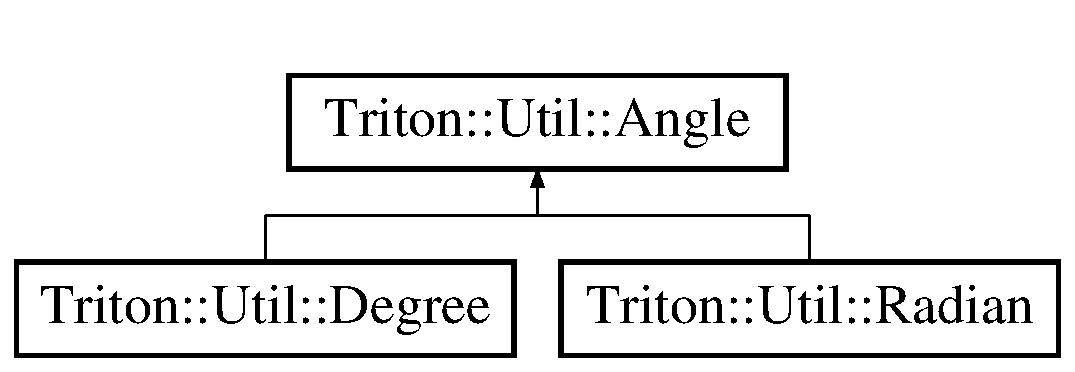
\includegraphics[height=2.000000cm]{struct_triton_1_1_util_1_1_angle}
\end{center}
\end{figure}
\subsection*{Public Types}
\begin{DoxyCompactItemize}
\item 
enum \hyperlink{group__lus__angle_ga38b6255184f9399841fa0b1d6bc4aa78}{Angle\+Type} \{ \hyperlink{group__lus__angle_gga38b6255184f9399841fa0b1d6bc4aa78ad5d37fcf38efdf957daee93ae0926788}{A\+N\+G\+L\+E}, 
\hyperlink{group__lus__angle_gga38b6255184f9399841fa0b1d6bc4aa78a65f1c5d48e03bd1de5960ba56db879dd}{D\+E\+G\+R\+E\+E}, 
\hyperlink{group__lus__angle_gga38b6255184f9399841fa0b1d6bc4aa78ada225beb0b39ac1224bf25804e15e08a}{R\+A\+D\+I\+A\+N}
 \}
\end{DoxyCompactItemize}
\subsection*{Public Member Functions}
\begin{DoxyCompactItemize}
\item 
virtual Rotation\+Type \hyperlink{struct_triton_1_1_util_1_1_angle_ac62cfbc48317457ff0992bc994f94f3e}{Get\+Rotation\+Type} ()
\end{DoxyCompactItemize}
\subsection*{Public Attributes}
\begin{DoxyCompactItemize}
\item 
float \hyperlink{struct_triton_1_1_util_1_1_angle_af7d7f20a28c150b09776a35bc1dae0c4}{ang}
\end{DoxyCompactItemize}


\subsection{Detailed Description}
A simple \hyperlink{struct_triton_1_1_util_1_1_angle}{Angle} object (practically an interface) 

Suggestion\+: Don\textquotesingle{}t use unless angle type will not matter 

Definition at line 19 of file angle.\+h.



\subsection{Member Function Documentation}
\hypertarget{struct_triton_1_1_util_1_1_angle_ac62cfbc48317457ff0992bc994f94f3e}{}\index{Triton\+::\+Util\+::\+Angle@{Triton\+::\+Util\+::\+Angle}!Get\+Rotation\+Type@{Get\+Rotation\+Type}}
\index{Get\+Rotation\+Type@{Get\+Rotation\+Type}!Triton\+::\+Util\+::\+Angle@{Triton\+::\+Util\+::\+Angle}}
\subsubsection[{Get\+Rotation\+Type}]{\setlength{\rightskip}{0pt plus 5cm}virtual Rotation\+Type Triton\+::\+Util\+::\+Angle\+::\+Get\+Rotation\+Type (
\begin{DoxyParamCaption}
{}
\end{DoxyParamCaption}
)\hspace{0.3cm}{\ttfamily [inline]}, {\ttfamily [virtual]}}\label{struct_triton_1_1_util_1_1_angle_ac62cfbc48317457ff0992bc994f94f3e}


Reimplemented in \hyperlink{struct_triton_1_1_util_1_1_radian_a75a4253af1ecb0bd75240fc604b8c61b}{Triton\+::\+Util\+::\+Radian}, and \hyperlink{struct_triton_1_1_util_1_1_degree_a31e2a2094c705e9195c1e8f076aa690d}{Triton\+::\+Util\+::\+Degree}.



Definition at line 30 of file angle.\+h.



\subsection{Member Data Documentation}
\hypertarget{struct_triton_1_1_util_1_1_angle_af7d7f20a28c150b09776a35bc1dae0c4}{}\index{Triton\+::\+Util\+::\+Angle@{Triton\+::\+Util\+::\+Angle}!ang@{ang}}
\index{ang@{ang}!Triton\+::\+Util\+::\+Angle@{Triton\+::\+Util\+::\+Angle}}
\subsubsection[{ang}]{\setlength{\rightskip}{0pt plus 5cm}float Triton\+::\+Util\+::\+Angle\+::ang}\label{struct_triton_1_1_util_1_1_angle_af7d7f20a28c150b09776a35bc1dae0c4}


Definition at line 28 of file angle.\+h.



The documentation for this struct was generated from the following file\+:\begin{DoxyCompactItemize}
\item 
util/\hyperlink{angle_8h}{angle.\+h}\end{DoxyCompactItemize}

\hypertarget{class_triton_1_1_util_1_1_basic_c_string}{}\section{Triton\+:\+:Util\+:\+:Basic\+C\+String$<$ char\+T $>$ Class Template Reference}
\label{class_triton_1_1_util_1_1_basic_c_string}\index{Triton\+::\+Util\+::\+Basic\+C\+String$<$ char\+T $>$@{Triton\+::\+Util\+::\+Basic\+C\+String$<$ char\+T $>$}}


{\ttfamily \#include $<$util.\+h$>$}

\subsection*{Public Member Functions}
\begin{DoxyCompactItemize}
\item 
void \hyperlink{class_triton_1_1_util_1_1_basic_c_string_a8cbf5157c160261d599a9b07e1cbbfd6}{Set\+String} (char\+T $\ast$str)
\item 
\hyperlink{class_triton_1_1_util_1_1_basic_c_string_a447877a937847af393e6781c0a7b20cc}{Base\+String} ()
\item 
\hyperlink{class_triton_1_1_util_1_1_basic_c_string_acbbe555dcaf7b19fafcead09229bad7d}{Base\+String} (char\+T $\ast$str)
\item 
const char\+T $\ast$ \hyperlink{class_triton_1_1_util_1_1_basic_c_string_a80c260353113320de1a6479c9acf00db}{c\+\_\+str} ()
\item 
const size\+\_\+t \hyperlink{class_triton_1_1_util_1_1_basic_c_string_afd89c0bcef5000a3b44c21e58686e170}{size} ()
\item 
\hyperlink{class_triton_1_1_util_1_1_basic_c_string_a447877a937847af393e6781c0a7b20cc}{Base\+String} \& \hyperlink{class_triton_1_1_util_1_1_basic_c_string_a84b969651c1cb694349a7d57964c8c96}{operator=} (const \hyperlink{class_triton_1_1_util_1_1_basic_c_string_a447877a937847af393e6781c0a7b20cc}{Base\+String} \&str)
\item 
\hyperlink{class_triton_1_1_util_1_1_basic_c_string_a447877a937847af393e6781c0a7b20cc}{Base\+String} \& \hyperlink{class_triton_1_1_util_1_1_basic_c_string_af25fdcef2f66c34dadb24aab6139c9b4}{operator=} (const char\+T $\ast$s)
\item 
\hyperlink{class_triton_1_1_util_1_1_basic_c_string_a447877a937847af393e6781c0a7b20cc}{Base\+String} \& \hyperlink{class_triton_1_1_util_1_1_basic_c_string_ab0b8c472b9b4cfdacbdb5f923dcd78bd}{operator=} (char\+T $\ast$s)
\item 
\hyperlink{class_triton_1_1_util_1_1_basic_c_string_a447877a937847af393e6781c0a7b20cc}{Base\+String} \& \hyperlink{class_triton_1_1_util_1_1_basic_c_string_ad8ed196fe36ea52cdaf94f77e1803b92}{operator=} (char\+T c)
\item 
char\+T \& \hyperlink{class_triton_1_1_util_1_1_basic_c_string_ae8eefe027c56f3eb0c2b35064c6e32b5}{operator\mbox{[}$\,$\mbox{]}} (size\+\_\+t pos)
\item 
const char\+T \& \hyperlink{class_triton_1_1_util_1_1_basic_c_string_aa1332902af0852069d3a87ef303380c6}{operator\mbox{[}$\,$\mbox{]}} (size\+\_\+t pos) const 
\item 
char \& \hyperlink{class_triton_1_1_util_1_1_basic_c_string_ad0ef2149ebba7f6b271d9c3449f7c0b8}{at} (size\+\_\+t pos)
\item 
const char \& \hyperlink{class_triton_1_1_util_1_1_basic_c_string_a039ed90fe8749739fd50fb020cc064b7}{at} (size\+\_\+t pos) const 
\item 
void \hyperlink{class_triton_1_1_util_1_1_basic_c_string_aca1796937dca8c0f5ef4a81c922e2c65}{clear} ()
\item 
bool \hyperlink{class_triton_1_1_util_1_1_basic_c_string_af20414a876cdae5143e07a82f81119ee}{empty} ()
\end{DoxyCompactItemize}


\subsection{Detailed Description}
\subsubsection*{template$<$class char\+T$>$class Triton\+::\+Util\+::\+Basic\+C\+String$<$ char\+T $>$}



Definition at line 15 of file util.\+h.



\subsection{Member Function Documentation}
\hypertarget{class_triton_1_1_util_1_1_basic_c_string_ad0ef2149ebba7f6b271d9c3449f7c0b8}{}\index{Triton\+::\+Util\+::\+Basic\+C\+String@{Triton\+::\+Util\+::\+Basic\+C\+String}!at@{at}}
\index{at@{at}!Triton\+::\+Util\+::\+Basic\+C\+String@{Triton\+::\+Util\+::\+Basic\+C\+String}}
\subsubsection[{at}]{\setlength{\rightskip}{0pt plus 5cm}template$<$class char\+T $>$ char\& {\bf Triton\+::\+Util\+::\+Basic\+C\+String}$<$ char\+T $>$\+::at (
\begin{DoxyParamCaption}
\item[{size\+\_\+t}]{pos}
\end{DoxyParamCaption}
)\hspace{0.3cm}{\ttfamily [inline]}}\label{class_triton_1_1_util_1_1_basic_c_string_ad0ef2149ebba7f6b271d9c3449f7c0b8}


Definition at line 86 of file util.\+h.

\hypertarget{class_triton_1_1_util_1_1_basic_c_string_a039ed90fe8749739fd50fb020cc064b7}{}\index{Triton\+::\+Util\+::\+Basic\+C\+String@{Triton\+::\+Util\+::\+Basic\+C\+String}!at@{at}}
\index{at@{at}!Triton\+::\+Util\+::\+Basic\+C\+String@{Triton\+::\+Util\+::\+Basic\+C\+String}}
\subsubsection[{at}]{\setlength{\rightskip}{0pt plus 5cm}template$<$class char\+T $>$ const char\& {\bf Triton\+::\+Util\+::\+Basic\+C\+String}$<$ char\+T $>$\+::at (
\begin{DoxyParamCaption}
\item[{size\+\_\+t}]{pos}
\end{DoxyParamCaption}
) const\hspace{0.3cm}{\ttfamily [inline]}}\label{class_triton_1_1_util_1_1_basic_c_string_a039ed90fe8749739fd50fb020cc064b7}


Definition at line 91 of file util.\+h.

\hypertarget{class_triton_1_1_util_1_1_basic_c_string_a447877a937847af393e6781c0a7b20cc}{}\index{Triton\+::\+Util\+::\+Basic\+C\+String@{Triton\+::\+Util\+::\+Basic\+C\+String}!Base\+String@{Base\+String}}
\index{Base\+String@{Base\+String}!Triton\+::\+Util\+::\+Basic\+C\+String@{Triton\+::\+Util\+::\+Basic\+C\+String}}
\subsubsection[{Base\+String}]{\setlength{\rightskip}{0pt plus 5cm}template$<$class char\+T $>$ {\bf Triton\+::\+Util\+::\+Basic\+C\+String}$<$ char\+T $>$\+::Base\+String (
\begin{DoxyParamCaption}
{}
\end{DoxyParamCaption}
)\hspace{0.3cm}{\ttfamily [inline]}}\label{class_triton_1_1_util_1_1_basic_c_string_a447877a937847af393e6781c0a7b20cc}


Definition at line 26 of file util.\+h.

\hypertarget{class_triton_1_1_util_1_1_basic_c_string_acbbe555dcaf7b19fafcead09229bad7d}{}\index{Triton\+::\+Util\+::\+Basic\+C\+String@{Triton\+::\+Util\+::\+Basic\+C\+String}!Base\+String@{Base\+String}}
\index{Base\+String@{Base\+String}!Triton\+::\+Util\+::\+Basic\+C\+String@{Triton\+::\+Util\+::\+Basic\+C\+String}}
\subsubsection[{Base\+String}]{\setlength{\rightskip}{0pt plus 5cm}template$<$class char\+T $>$ {\bf Triton\+::\+Util\+::\+Basic\+C\+String}$<$ char\+T $>$\+::Base\+String (
\begin{DoxyParamCaption}
\item[{char\+T $\ast$}]{str}
\end{DoxyParamCaption}
)\hspace{0.3cm}{\ttfamily [inline]}}\label{class_triton_1_1_util_1_1_basic_c_string_acbbe555dcaf7b19fafcead09229bad7d}


Definition at line 32 of file util.\+h.

\hypertarget{class_triton_1_1_util_1_1_basic_c_string_a80c260353113320de1a6479c9acf00db}{}\index{Triton\+::\+Util\+::\+Basic\+C\+String@{Triton\+::\+Util\+::\+Basic\+C\+String}!c\+\_\+str@{c\+\_\+str}}
\index{c\+\_\+str@{c\+\_\+str}!Triton\+::\+Util\+::\+Basic\+C\+String@{Triton\+::\+Util\+::\+Basic\+C\+String}}
\subsubsection[{c\+\_\+str}]{\setlength{\rightskip}{0pt plus 5cm}template$<$class char\+T $>$ const char\+T$\ast$ {\bf Triton\+::\+Util\+::\+Basic\+C\+String}$<$ char\+T $>$\+::c\+\_\+str (
\begin{DoxyParamCaption}
{}
\end{DoxyParamCaption}
)\hspace{0.3cm}{\ttfamily [inline]}}\label{class_triton_1_1_util_1_1_basic_c_string_a80c260353113320de1a6479c9acf00db}


Definition at line 37 of file util.\+h.

\hypertarget{class_triton_1_1_util_1_1_basic_c_string_aca1796937dca8c0f5ef4a81c922e2c65}{}\index{Triton\+::\+Util\+::\+Basic\+C\+String@{Triton\+::\+Util\+::\+Basic\+C\+String}!clear@{clear}}
\index{clear@{clear}!Triton\+::\+Util\+::\+Basic\+C\+String@{Triton\+::\+Util\+::\+Basic\+C\+String}}
\subsubsection[{clear}]{\setlength{\rightskip}{0pt plus 5cm}template$<$class char\+T $>$ void {\bf Triton\+::\+Util\+::\+Basic\+C\+String}$<$ char\+T $>$\+::clear (
\begin{DoxyParamCaption}
{}
\end{DoxyParamCaption}
)\hspace{0.3cm}{\ttfamily [inline]}}\label{class_triton_1_1_util_1_1_basic_c_string_aca1796937dca8c0f5ef4a81c922e2c65}


Definition at line 96 of file util.\+h.

\hypertarget{class_triton_1_1_util_1_1_basic_c_string_af20414a876cdae5143e07a82f81119ee}{}\index{Triton\+::\+Util\+::\+Basic\+C\+String@{Triton\+::\+Util\+::\+Basic\+C\+String}!empty@{empty}}
\index{empty@{empty}!Triton\+::\+Util\+::\+Basic\+C\+String@{Triton\+::\+Util\+::\+Basic\+C\+String}}
\subsubsection[{empty}]{\setlength{\rightskip}{0pt plus 5cm}template$<$class char\+T $>$ bool {\bf Triton\+::\+Util\+::\+Basic\+C\+String}$<$ char\+T $>$\+::empty (
\begin{DoxyParamCaption}
{}
\end{DoxyParamCaption}
)\hspace{0.3cm}{\ttfamily [inline]}}\label{class_triton_1_1_util_1_1_basic_c_string_af20414a876cdae5143e07a82f81119ee}


Definition at line 101 of file util.\+h.

\hypertarget{class_triton_1_1_util_1_1_basic_c_string_a84b969651c1cb694349a7d57964c8c96}{}\index{Triton\+::\+Util\+::\+Basic\+C\+String@{Triton\+::\+Util\+::\+Basic\+C\+String}!operator=@{operator=}}
\index{operator=@{operator=}!Triton\+::\+Util\+::\+Basic\+C\+String@{Triton\+::\+Util\+::\+Basic\+C\+String}}
\subsubsection[{operator=}]{\setlength{\rightskip}{0pt plus 5cm}template$<$class char\+T $>$ {\bf Base\+String}\& {\bf Triton\+::\+Util\+::\+Basic\+C\+String}$<$ char\+T $>$\+::operator= (
\begin{DoxyParamCaption}
\item[{const {\bf Base\+String} \&}]{str}
\end{DoxyParamCaption}
)\hspace{0.3cm}{\ttfamily [inline]}}\label{class_triton_1_1_util_1_1_basic_c_string_a84b969651c1cb694349a7d57964c8c96}


Definition at line 47 of file util.\+h.

\hypertarget{class_triton_1_1_util_1_1_basic_c_string_af25fdcef2f66c34dadb24aab6139c9b4}{}\index{Triton\+::\+Util\+::\+Basic\+C\+String@{Triton\+::\+Util\+::\+Basic\+C\+String}!operator=@{operator=}}
\index{operator=@{operator=}!Triton\+::\+Util\+::\+Basic\+C\+String@{Triton\+::\+Util\+::\+Basic\+C\+String}}
\subsubsection[{operator=}]{\setlength{\rightskip}{0pt plus 5cm}template$<$class char\+T $>$ {\bf Base\+String}\& {\bf Triton\+::\+Util\+::\+Basic\+C\+String}$<$ char\+T $>$\+::operator= (
\begin{DoxyParamCaption}
\item[{const char\+T $\ast$}]{s}
\end{DoxyParamCaption}
)\hspace{0.3cm}{\ttfamily [inline]}}\label{class_triton_1_1_util_1_1_basic_c_string_af25fdcef2f66c34dadb24aab6139c9b4}


Definition at line 53 of file util.\+h.

\hypertarget{class_triton_1_1_util_1_1_basic_c_string_ab0b8c472b9b4cfdacbdb5f923dcd78bd}{}\index{Triton\+::\+Util\+::\+Basic\+C\+String@{Triton\+::\+Util\+::\+Basic\+C\+String}!operator=@{operator=}}
\index{operator=@{operator=}!Triton\+::\+Util\+::\+Basic\+C\+String@{Triton\+::\+Util\+::\+Basic\+C\+String}}
\subsubsection[{operator=}]{\setlength{\rightskip}{0pt plus 5cm}template$<$class char\+T $>$ {\bf Base\+String}\& {\bf Triton\+::\+Util\+::\+Basic\+C\+String}$<$ char\+T $>$\+::operator= (
\begin{DoxyParamCaption}
\item[{char\+T $\ast$}]{s}
\end{DoxyParamCaption}
)\hspace{0.3cm}{\ttfamily [inline]}}\label{class_triton_1_1_util_1_1_basic_c_string_ab0b8c472b9b4cfdacbdb5f923dcd78bd}


Definition at line 61 of file util.\+h.

\hypertarget{class_triton_1_1_util_1_1_basic_c_string_ad8ed196fe36ea52cdaf94f77e1803b92}{}\index{Triton\+::\+Util\+::\+Basic\+C\+String@{Triton\+::\+Util\+::\+Basic\+C\+String}!operator=@{operator=}}
\index{operator=@{operator=}!Triton\+::\+Util\+::\+Basic\+C\+String@{Triton\+::\+Util\+::\+Basic\+C\+String}}
\subsubsection[{operator=}]{\setlength{\rightskip}{0pt plus 5cm}template$<$class char\+T $>$ {\bf Base\+String}\& {\bf Triton\+::\+Util\+::\+Basic\+C\+String}$<$ char\+T $>$\+::operator= (
\begin{DoxyParamCaption}
\item[{char\+T}]{c}
\end{DoxyParamCaption}
)\hspace{0.3cm}{\ttfamily [inline]}}\label{class_triton_1_1_util_1_1_basic_c_string_ad8ed196fe36ea52cdaf94f77e1803b92}


Definition at line 67 of file util.\+h.

\hypertarget{class_triton_1_1_util_1_1_basic_c_string_ae8eefe027c56f3eb0c2b35064c6e32b5}{}\index{Triton\+::\+Util\+::\+Basic\+C\+String@{Triton\+::\+Util\+::\+Basic\+C\+String}!operator\mbox{[}$\,$\mbox{]}@{operator[]}}
\index{operator\mbox{[}$\,$\mbox{]}@{operator[]}!Triton\+::\+Util\+::\+Basic\+C\+String@{Triton\+::\+Util\+::\+Basic\+C\+String}}
\subsubsection[{operator[]}]{\setlength{\rightskip}{0pt plus 5cm}template$<$class char\+T $>$ char\+T\& {\bf Triton\+::\+Util\+::\+Basic\+C\+String}$<$ char\+T $>$\+::operator\mbox{[}$\,$\mbox{]} (
\begin{DoxyParamCaption}
\item[{size\+\_\+t}]{pos}
\end{DoxyParamCaption}
)\hspace{0.3cm}{\ttfamily [inline]}}\label{class_triton_1_1_util_1_1_basic_c_string_ae8eefe027c56f3eb0c2b35064c6e32b5}


Definition at line 74 of file util.\+h.

\hypertarget{class_triton_1_1_util_1_1_basic_c_string_aa1332902af0852069d3a87ef303380c6}{}\index{Triton\+::\+Util\+::\+Basic\+C\+String@{Triton\+::\+Util\+::\+Basic\+C\+String}!operator\mbox{[}$\,$\mbox{]}@{operator[]}}
\index{operator\mbox{[}$\,$\mbox{]}@{operator[]}!Triton\+::\+Util\+::\+Basic\+C\+String@{Triton\+::\+Util\+::\+Basic\+C\+String}}
\subsubsection[{operator[]}]{\setlength{\rightskip}{0pt plus 5cm}template$<$class char\+T $>$ const char\+T\& {\bf Triton\+::\+Util\+::\+Basic\+C\+String}$<$ char\+T $>$\+::operator\mbox{[}$\,$\mbox{]} (
\begin{DoxyParamCaption}
\item[{size\+\_\+t}]{pos}
\end{DoxyParamCaption}
) const\hspace{0.3cm}{\ttfamily [inline]}}\label{class_triton_1_1_util_1_1_basic_c_string_aa1332902af0852069d3a87ef303380c6}


Definition at line 80 of file util.\+h.

\hypertarget{class_triton_1_1_util_1_1_basic_c_string_a8cbf5157c160261d599a9b07e1cbbfd6}{}\index{Triton\+::\+Util\+::\+Basic\+C\+String@{Triton\+::\+Util\+::\+Basic\+C\+String}!Set\+String@{Set\+String}}
\index{Set\+String@{Set\+String}!Triton\+::\+Util\+::\+Basic\+C\+String@{Triton\+::\+Util\+::\+Basic\+C\+String}}
\subsubsection[{Set\+String}]{\setlength{\rightskip}{0pt plus 5cm}template$<$class char\+T $>$ void {\bf Triton\+::\+Util\+::\+Basic\+C\+String}$<$ char\+T $>$\+::Set\+String (
\begin{DoxyParamCaption}
\item[{char\+T $\ast$}]{str}
\end{DoxyParamCaption}
)\hspace{0.3cm}{\ttfamily [inline]}}\label{class_triton_1_1_util_1_1_basic_c_string_a8cbf5157c160261d599a9b07e1cbbfd6}


Definition at line 20 of file util.\+h.

\hypertarget{class_triton_1_1_util_1_1_basic_c_string_afd89c0bcef5000a3b44c21e58686e170}{}\index{Triton\+::\+Util\+::\+Basic\+C\+String@{Triton\+::\+Util\+::\+Basic\+C\+String}!size@{size}}
\index{size@{size}!Triton\+::\+Util\+::\+Basic\+C\+String@{Triton\+::\+Util\+::\+Basic\+C\+String}}
\subsubsection[{size}]{\setlength{\rightskip}{0pt plus 5cm}template$<$class char\+T $>$ const size\+\_\+t {\bf Triton\+::\+Util\+::\+Basic\+C\+String}$<$ char\+T $>$\+::size (
\begin{DoxyParamCaption}
{}
\end{DoxyParamCaption}
)\hspace{0.3cm}{\ttfamily [inline]}}\label{class_triton_1_1_util_1_1_basic_c_string_afd89c0bcef5000a3b44c21e58686e170}


Definition at line 42 of file util.\+h.



The documentation for this class was generated from the following file\+:\begin{DoxyCompactItemize}
\item 
util/\hyperlink{util_2util_8h}{util.\+h}\end{DoxyCompactItemize}

\hypertarget{class_tri_1_1_graphic_1_1_camera}{}\section{Tri\+:\+:Graphic\+:\+:Camera Class Reference}
\label{class_tri_1_1_graphic_1_1_camera}\index{Tri\+::\+Graphic\+::\+Camera@{Tri\+::\+Graphic\+::\+Camera}}


{\ttfamily \#include $<$render.\+h$>$}

\subsection*{Public Member Functions}
\begin{DoxyCompactItemize}
\item 
\hyperlink{class_tri_1_1_graphic_1_1_camera_aa2ba829b31e486b2028d6b517017e8cd}{Camera} (Util\+::\+Vec3$<$ double $>$ position, Util\+::\+Vec3$<$ Util\+::\+Radian $>$ rotation, Util\+::\+Degree fov=Util\+::\+Degree(60))
\item 
virtual void \hyperlink{class_tri_1_1_graphic_1_1_camera_aa68fd9c51d56bb999364a13c774998f4}{Update} (int tick)
\item 
\hyperlink{namespace_tri_1_1_graphic_a7b3538cdaff9bf96489c56a4f48a5f9a}{Mat4} \hyperlink{class_tri_1_1_graphic_1_1_camera_a0aa6799cf1a3541c3e17c010a4f65f99}{Get\+View\+Matrix} ()
\item 
void \hyperlink{class_tri_1_1_graphic_1_1_camera_a1b3bd9b5923e6d72db9521212fb8855d}{Rotate} (Util\+::\+Vec2$<$ Angle $>$ rotation)
\item 
void \hyperlink{class_tri_1_1_graphic_1_1_camera_a589dd8cde32e62172946f532c816d3c5}{Move\+To} (Util\+::\+Vec2$<$ double $>$ position)
\item 
void \hyperlink{class_tri_1_1_graphic_1_1_camera_abc66a18ab619979fc57858c0ec8262ed}{Set\+Fov} (Util\+::\+Degree fov)
\item 
void \hyperlink{class_tri_1_1_graphic_1_1_camera_afd94099a3837504a1a26c82687e1a1ae}{Set\+Is\+Upside\+Down} (bool face\+Up)
\item 
Util\+::\+Vec3$<$ double $>$ \hyperlink{class_tri_1_1_graphic_1_1_camera_ab65dc5d24d096e2b3da164d677c80412}{Get\+Position} ()
\item 
Util\+::\+Vec3$<$ Util\+::\+Radian $>$ \hyperlink{class_tri_1_1_graphic_1_1_camera_a9c212c2c5adc0ac98066801c2f88754c}{Get\+Rotation} ()
\item 
float \hyperlink{class_tri_1_1_graphic_1_1_camera_af300bae226e0213af31e97eaf2c13068}{Get\+Fov} ()
\item 
bool \hyperlink{class_tri_1_1_graphic_1_1_camera_a92e5b27f0204116e1fa75e37ade5e181}{Is\+Upside\+Down} ()
\end{DoxyCompactItemize}
\subsection*{Protected Member Functions}
\begin{DoxyCompactItemize}
\item 
virtual void \hyperlink{class_tri_1_1_graphic_1_1_camera_a37b6d6a2a0cd8c353d73f4c9a3e6c6dc}{on\+Rotate} (Util\+::\+Vec2$<$ Angle $>$ \&r\+Rotation)
\item 
virtual void \hyperlink{class_tri_1_1_graphic_1_1_camera_a310dd53bc8771676bbe9cfc29c28db6a}{on\+Move} (Util\+::\+Vec2$<$ double $>$ \&r\+Position)
\end{DoxyCompactItemize}
\subsection*{Protected Attributes}
\begin{DoxyCompactItemize}
\item 
Util\+::\+Vec3$<$ double $>$ \hyperlink{class_tri_1_1_graphic_1_1_camera_ad813eaa168e21644d89f69cd255f0643}{m\+Position}
\item 
Util\+::\+Vec3$<$ Util\+::\+Radian $>$ \hyperlink{class_tri_1_1_graphic_1_1_camera_a81ca7e49b98bfc6517200ccd2ff89098}{m\+Rotation}
\item 
Util\+::\+Degree \hyperlink{class_tri_1_1_graphic_1_1_camera_a03fa8565fd7780168daba8acecf3a632}{m\+Fov}
\item 
bool \hyperlink{class_tri_1_1_graphic_1_1_camera_a2488f8451d905297a6085529f1777de9}{m\+Is\+Upside\+Down} = false
\end{DoxyCompactItemize}


\subsection{Detailed Description}


Definition at line 12 of file render.\+h.



\subsection{Constructor \& Destructor Documentation}
\hypertarget{class_tri_1_1_graphic_1_1_camera_aa2ba829b31e486b2028d6b517017e8cd}{}\index{Tri\+::\+Graphic\+::\+Camera@{Tri\+::\+Graphic\+::\+Camera}!Camera@{Camera}}
\index{Camera@{Camera}!Tri\+::\+Graphic\+::\+Camera@{Tri\+::\+Graphic\+::\+Camera}}
\subsubsection[{Camera}]{\setlength{\rightskip}{0pt plus 5cm}Tri\+::\+Graphic\+::\+Camera\+::\+Camera (
\begin{DoxyParamCaption}
\item[{Util\+::\+Vec3$<$ double $>$}]{position, }
\item[{Util\+::\+Vec3$<$ Util\+::\+Radian $>$}]{rotation, }
\item[{Util\+::\+Degree}]{fov = {\ttfamily Util\+:\+:Degree(60)}}
\end{DoxyParamCaption}
)}\label{class_tri_1_1_graphic_1_1_camera_aa2ba829b31e486b2028d6b517017e8cd}


\subsection{Member Function Documentation}
\hypertarget{class_tri_1_1_graphic_1_1_camera_af300bae226e0213af31e97eaf2c13068}{}\index{Tri\+::\+Graphic\+::\+Camera@{Tri\+::\+Graphic\+::\+Camera}!Get\+Fov@{Get\+Fov}}
\index{Get\+Fov@{Get\+Fov}!Tri\+::\+Graphic\+::\+Camera@{Tri\+::\+Graphic\+::\+Camera}}
\subsubsection[{Get\+Fov}]{\setlength{\rightskip}{0pt plus 5cm}float Tri\+::\+Graphic\+::\+Camera\+::\+Get\+Fov (
\begin{DoxyParamCaption}
{}
\end{DoxyParamCaption}
)}\label{class_tri_1_1_graphic_1_1_camera_af300bae226e0213af31e97eaf2c13068}
\hypertarget{class_tri_1_1_graphic_1_1_camera_ab65dc5d24d096e2b3da164d677c80412}{}\index{Tri\+::\+Graphic\+::\+Camera@{Tri\+::\+Graphic\+::\+Camera}!Get\+Position@{Get\+Position}}
\index{Get\+Position@{Get\+Position}!Tri\+::\+Graphic\+::\+Camera@{Tri\+::\+Graphic\+::\+Camera}}
\subsubsection[{Get\+Position}]{\setlength{\rightskip}{0pt plus 5cm}Util\+::\+Vec3$<$double$>$ Tri\+::\+Graphic\+::\+Camera\+::\+Get\+Position (
\begin{DoxyParamCaption}
{}
\end{DoxyParamCaption}
)}\label{class_tri_1_1_graphic_1_1_camera_ab65dc5d24d096e2b3da164d677c80412}
\hypertarget{class_tri_1_1_graphic_1_1_camera_a9c212c2c5adc0ac98066801c2f88754c}{}\index{Tri\+::\+Graphic\+::\+Camera@{Tri\+::\+Graphic\+::\+Camera}!Get\+Rotation@{Get\+Rotation}}
\index{Get\+Rotation@{Get\+Rotation}!Tri\+::\+Graphic\+::\+Camera@{Tri\+::\+Graphic\+::\+Camera}}
\subsubsection[{Get\+Rotation}]{\setlength{\rightskip}{0pt plus 5cm}Util\+::\+Vec3$<$Util\+::\+Radian$>$ Tri\+::\+Graphic\+::\+Camera\+::\+Get\+Rotation (
\begin{DoxyParamCaption}
{}
\end{DoxyParamCaption}
)}\label{class_tri_1_1_graphic_1_1_camera_a9c212c2c5adc0ac98066801c2f88754c}
\hypertarget{class_tri_1_1_graphic_1_1_camera_a0aa6799cf1a3541c3e17c010a4f65f99}{}\index{Tri\+::\+Graphic\+::\+Camera@{Tri\+::\+Graphic\+::\+Camera}!Get\+View\+Matrix@{Get\+View\+Matrix}}
\index{Get\+View\+Matrix@{Get\+View\+Matrix}!Tri\+::\+Graphic\+::\+Camera@{Tri\+::\+Graphic\+::\+Camera}}
\subsubsection[{Get\+View\+Matrix}]{\setlength{\rightskip}{0pt plus 5cm}{\bf Mat4} Tri\+::\+Graphic\+::\+Camera\+::\+Get\+View\+Matrix (
\begin{DoxyParamCaption}
{}
\end{DoxyParamCaption}
)}\label{class_tri_1_1_graphic_1_1_camera_a0aa6799cf1a3541c3e17c010a4f65f99}
\hypertarget{class_tri_1_1_graphic_1_1_camera_a92e5b27f0204116e1fa75e37ade5e181}{}\index{Tri\+::\+Graphic\+::\+Camera@{Tri\+::\+Graphic\+::\+Camera}!Is\+Upside\+Down@{Is\+Upside\+Down}}
\index{Is\+Upside\+Down@{Is\+Upside\+Down}!Tri\+::\+Graphic\+::\+Camera@{Tri\+::\+Graphic\+::\+Camera}}
\subsubsection[{Is\+Upside\+Down}]{\setlength{\rightskip}{0pt plus 5cm}bool Tri\+::\+Graphic\+::\+Camera\+::\+Is\+Upside\+Down (
\begin{DoxyParamCaption}
{}
\end{DoxyParamCaption}
)}\label{class_tri_1_1_graphic_1_1_camera_a92e5b27f0204116e1fa75e37ade5e181}
\hypertarget{class_tri_1_1_graphic_1_1_camera_a589dd8cde32e62172946f532c816d3c5}{}\index{Tri\+::\+Graphic\+::\+Camera@{Tri\+::\+Graphic\+::\+Camera}!Move\+To@{Move\+To}}
\index{Move\+To@{Move\+To}!Tri\+::\+Graphic\+::\+Camera@{Tri\+::\+Graphic\+::\+Camera}}
\subsubsection[{Move\+To}]{\setlength{\rightskip}{0pt plus 5cm}void Tri\+::\+Graphic\+::\+Camera\+::\+Move\+To (
\begin{DoxyParamCaption}
\item[{Util\+::\+Vec2$<$ double $>$}]{position}
\end{DoxyParamCaption}
)}\label{class_tri_1_1_graphic_1_1_camera_a589dd8cde32e62172946f532c816d3c5}
\hypertarget{class_tri_1_1_graphic_1_1_camera_a310dd53bc8771676bbe9cfc29c28db6a}{}\index{Tri\+::\+Graphic\+::\+Camera@{Tri\+::\+Graphic\+::\+Camera}!on\+Move@{on\+Move}}
\index{on\+Move@{on\+Move}!Tri\+::\+Graphic\+::\+Camera@{Tri\+::\+Graphic\+::\+Camera}}
\subsubsection[{on\+Move}]{\setlength{\rightskip}{0pt plus 5cm}virtual void Tri\+::\+Graphic\+::\+Camera\+::on\+Move (
\begin{DoxyParamCaption}
\item[{Util\+::\+Vec2$<$ double $>$ \&}]{r\+Position}
\end{DoxyParamCaption}
)\hspace{0.3cm}{\ttfamily [inline]}, {\ttfamily [protected]}, {\ttfamily [virtual]}}\label{class_tri_1_1_graphic_1_1_camera_a310dd53bc8771676bbe9cfc29c28db6a}


Definition at line 21 of file render.\+h.

\hypertarget{class_tri_1_1_graphic_1_1_camera_a37b6d6a2a0cd8c353d73f4c9a3e6c6dc}{}\index{Tri\+::\+Graphic\+::\+Camera@{Tri\+::\+Graphic\+::\+Camera}!on\+Rotate@{on\+Rotate}}
\index{on\+Rotate@{on\+Rotate}!Tri\+::\+Graphic\+::\+Camera@{Tri\+::\+Graphic\+::\+Camera}}
\subsubsection[{on\+Rotate}]{\setlength{\rightskip}{0pt plus 5cm}virtual void Tri\+::\+Graphic\+::\+Camera\+::on\+Rotate (
\begin{DoxyParamCaption}
\item[{Util\+::\+Vec2$<$ Angle $>$ \&}]{r\+Rotation}
\end{DoxyParamCaption}
)\hspace{0.3cm}{\ttfamily [inline]}, {\ttfamily [protected]}, {\ttfamily [virtual]}}\label{class_tri_1_1_graphic_1_1_camera_a37b6d6a2a0cd8c353d73f4c9a3e6c6dc}


Definition at line 20 of file render.\+h.

\hypertarget{class_tri_1_1_graphic_1_1_camera_a1b3bd9b5923e6d72db9521212fb8855d}{}\index{Tri\+::\+Graphic\+::\+Camera@{Tri\+::\+Graphic\+::\+Camera}!Rotate@{Rotate}}
\index{Rotate@{Rotate}!Tri\+::\+Graphic\+::\+Camera@{Tri\+::\+Graphic\+::\+Camera}}
\subsubsection[{Rotate}]{\setlength{\rightskip}{0pt plus 5cm}void Tri\+::\+Graphic\+::\+Camera\+::\+Rotate (
\begin{DoxyParamCaption}
\item[{Util\+::\+Vec2$<$ Angle $>$}]{rotation}
\end{DoxyParamCaption}
)}\label{class_tri_1_1_graphic_1_1_camera_a1b3bd9b5923e6d72db9521212fb8855d}
\hypertarget{class_tri_1_1_graphic_1_1_camera_abc66a18ab619979fc57858c0ec8262ed}{}\index{Tri\+::\+Graphic\+::\+Camera@{Tri\+::\+Graphic\+::\+Camera}!Set\+Fov@{Set\+Fov}}
\index{Set\+Fov@{Set\+Fov}!Tri\+::\+Graphic\+::\+Camera@{Tri\+::\+Graphic\+::\+Camera}}
\subsubsection[{Set\+Fov}]{\setlength{\rightskip}{0pt plus 5cm}void Tri\+::\+Graphic\+::\+Camera\+::\+Set\+Fov (
\begin{DoxyParamCaption}
\item[{Util\+::\+Degree}]{fov}
\end{DoxyParamCaption}
)}\label{class_tri_1_1_graphic_1_1_camera_abc66a18ab619979fc57858c0ec8262ed}
\hypertarget{class_tri_1_1_graphic_1_1_camera_afd94099a3837504a1a26c82687e1a1ae}{}\index{Tri\+::\+Graphic\+::\+Camera@{Tri\+::\+Graphic\+::\+Camera}!Set\+Is\+Upside\+Down@{Set\+Is\+Upside\+Down}}
\index{Set\+Is\+Upside\+Down@{Set\+Is\+Upside\+Down}!Tri\+::\+Graphic\+::\+Camera@{Tri\+::\+Graphic\+::\+Camera}}
\subsubsection[{Set\+Is\+Upside\+Down}]{\setlength{\rightskip}{0pt plus 5cm}void Tri\+::\+Graphic\+::\+Camera\+::\+Set\+Is\+Upside\+Down (
\begin{DoxyParamCaption}
\item[{bool}]{face\+Up}
\end{DoxyParamCaption}
)}\label{class_tri_1_1_graphic_1_1_camera_afd94099a3837504a1a26c82687e1a1ae}
\hypertarget{class_tri_1_1_graphic_1_1_camera_aa68fd9c51d56bb999364a13c774998f4}{}\index{Tri\+::\+Graphic\+::\+Camera@{Tri\+::\+Graphic\+::\+Camera}!Update@{Update}}
\index{Update@{Update}!Tri\+::\+Graphic\+::\+Camera@{Tri\+::\+Graphic\+::\+Camera}}
\subsubsection[{Update}]{\setlength{\rightskip}{0pt plus 5cm}virtual void Tri\+::\+Graphic\+::\+Camera\+::\+Update (
\begin{DoxyParamCaption}
\item[{int}]{tick}
\end{DoxyParamCaption}
)\hspace{0.3cm}{\ttfamily [inline]}, {\ttfamily [virtual]}}\label{class_tri_1_1_graphic_1_1_camera_aa68fd9c51d56bb999364a13c774998f4}


Definition at line 29 of file render.\+h.



\subsection{Member Data Documentation}
\hypertarget{class_tri_1_1_graphic_1_1_camera_a03fa8565fd7780168daba8acecf3a632}{}\index{Tri\+::\+Graphic\+::\+Camera@{Tri\+::\+Graphic\+::\+Camera}!m\+Fov@{m\+Fov}}
\index{m\+Fov@{m\+Fov}!Tri\+::\+Graphic\+::\+Camera@{Tri\+::\+Graphic\+::\+Camera}}
\subsubsection[{m\+Fov}]{\setlength{\rightskip}{0pt plus 5cm}Util\+::\+Degree Tri\+::\+Graphic\+::\+Camera\+::m\+Fov\hspace{0.3cm}{\ttfamily [protected]}}\label{class_tri_1_1_graphic_1_1_camera_a03fa8565fd7780168daba8acecf3a632}


Definition at line 17 of file render.\+h.

\hypertarget{class_tri_1_1_graphic_1_1_camera_a2488f8451d905297a6085529f1777de9}{}\index{Tri\+::\+Graphic\+::\+Camera@{Tri\+::\+Graphic\+::\+Camera}!m\+Is\+Upside\+Down@{m\+Is\+Upside\+Down}}
\index{m\+Is\+Upside\+Down@{m\+Is\+Upside\+Down}!Tri\+::\+Graphic\+::\+Camera@{Tri\+::\+Graphic\+::\+Camera}}
\subsubsection[{m\+Is\+Upside\+Down}]{\setlength{\rightskip}{0pt plus 5cm}bool Tri\+::\+Graphic\+::\+Camera\+::m\+Is\+Upside\+Down = false\hspace{0.3cm}{\ttfamily [protected]}}\label{class_tri_1_1_graphic_1_1_camera_a2488f8451d905297a6085529f1777de9}


Definition at line 18 of file render.\+h.

\hypertarget{class_tri_1_1_graphic_1_1_camera_ad813eaa168e21644d89f69cd255f0643}{}\index{Tri\+::\+Graphic\+::\+Camera@{Tri\+::\+Graphic\+::\+Camera}!m\+Position@{m\+Position}}
\index{m\+Position@{m\+Position}!Tri\+::\+Graphic\+::\+Camera@{Tri\+::\+Graphic\+::\+Camera}}
\subsubsection[{m\+Position}]{\setlength{\rightskip}{0pt plus 5cm}Util\+::\+Vec3$<$double$>$ Tri\+::\+Graphic\+::\+Camera\+::m\+Position\hspace{0.3cm}{\ttfamily [protected]}}\label{class_tri_1_1_graphic_1_1_camera_ad813eaa168e21644d89f69cd255f0643}


Definition at line 15 of file render.\+h.

\hypertarget{class_tri_1_1_graphic_1_1_camera_a81ca7e49b98bfc6517200ccd2ff89098}{}\index{Tri\+::\+Graphic\+::\+Camera@{Tri\+::\+Graphic\+::\+Camera}!m\+Rotation@{m\+Rotation}}
\index{m\+Rotation@{m\+Rotation}!Tri\+::\+Graphic\+::\+Camera@{Tri\+::\+Graphic\+::\+Camera}}
\subsubsection[{m\+Rotation}]{\setlength{\rightskip}{0pt plus 5cm}Util\+::\+Vec3$<$Util\+::\+Radian$>$ Tri\+::\+Graphic\+::\+Camera\+::m\+Rotation\hspace{0.3cm}{\ttfamily [protected]}}\label{class_tri_1_1_graphic_1_1_camera_a81ca7e49b98bfc6517200ccd2ff89098}


Definition at line 16 of file render.\+h.



The documentation for this class was generated from the following file\+:\begin{DoxyCompactItemize}
\item 
graphic/\hyperlink{render_8h}{render.\+h}\end{DoxyCompactItemize}

\hypertarget{class_triton_1_1_util_1_1_c_string}{}\section{Triton\+:\+:Util\+:\+:C\+String Class Reference}
\label{class_triton_1_1_util_1_1_c_string}\index{Triton\+::\+Util\+::\+C\+String@{Triton\+::\+Util\+::\+C\+String}}


{\ttfamily \#include $<$string.\+h$>$}

\subsection*{Public Member Functions}
\begin{DoxyCompactItemize}
\item 
void \hyperlink{class_triton_1_1_util_1_1_c_string_a2d99993046d41bc60d8a5bf173f0ef23}{Set\+String} (char $\ast$str)
\item 
void \hyperlink{class_triton_1_1_util_1_1_c_string_aa3427f97f76ded12150515dacee85731}{Set\+String} (const char $\ast$str)
\item 
void \hyperlink{class_triton_1_1_util_1_1_c_string_a7e2e7725fcc28854f9a2537ef868ea6e}{Set\+String} (std\+::string str)
\item 
void \hyperlink{class_triton_1_1_util_1_1_c_string_a7b016d657350f3c1284003eff2a83481}{Set\+String} (\hyperlink{class_triton_1_1_util_1_1_c_string}{C\+String} str)
\item 
void \hyperlink{class_triton_1_1_util_1_1_c_string_ad4b79623a0f4951163bd9012d63aab66}{Set\+String} (std\+::string $\ast$str)
\item 
void \hyperlink{class_triton_1_1_util_1_1_c_string_a524b917014029845222d5d9f9da52220}{Set\+String} (\hyperlink{class_triton_1_1_util_1_1_c_string}{C\+String} $\ast$str)
\item 
void \hyperlink{class_triton_1_1_util_1_1_c_string_abd0642e3763d2f249936650eb10b6df9}{Set\+String} (char str)
\item 
\hyperlink{class_triton_1_1_util_1_1_c_string_a3f5225befe1c5d044ab4c1a447e6b319}{C\+String} ()
\item 
{\footnotesize template$<$typename str\+T $>$ }\\\hyperlink{class_triton_1_1_util_1_1_c_string_a7d9bdd0c12463b9d571824e5ffdb0fc8}{C\+String} (str\+T str)
\item 
{\footnotesize template$<$typename str\+T $>$ }\\\hyperlink{class_triton_1_1_util_1_1_c_string_a132b944a6c13bc90401e48d7dd3730c0}{C\+String} (str\+T $\ast$str)
\item 
const char $\ast$ \hyperlink{class_triton_1_1_util_1_1_c_string_a48b57cd50721dc8968aacf4a6ac3cb6e}{c\+\_\+str} () const 
\item 
const size\+\_\+t \hyperlink{class_triton_1_1_util_1_1_c_string_ad557f15db25da1ee60ec54db1cfa2239}{size} () const 
\item 
{\footnotesize template$<$typename char\+T $>$ }\\\hyperlink{class_triton_1_1_util_1_1_c_string}{C\+String} \& \hyperlink{class_triton_1_1_util_1_1_c_string_a2d75b9caa4eb2c910c8dbb281e56d5f5}{operator=} (char\+T $\ast$s)
\item 
{\footnotesize template$<$typename char\+T $>$ }\\\hyperlink{class_triton_1_1_util_1_1_c_string}{C\+String} \& \hyperlink{class_triton_1_1_util_1_1_c_string_ac4876a014373694f2c3bc33fd66df5d8}{operator=} (char\+T s)
\item 
char \& \hyperlink{class_triton_1_1_util_1_1_c_string_aea5765384d6881c7b1326d8ece716dbd}{operator\mbox{[}$\,$\mbox{]}} (size\+\_\+t pos)
\item 
char \& \hyperlink{class_triton_1_1_util_1_1_c_string_a6d74b6d9eacb410bed320ec94068b7e8}{operator\mbox{[}$\,$\mbox{]}} (size\+\_\+t pos) const 
\item 
char \& \hyperlink{class_triton_1_1_util_1_1_c_string_ae02e05e16f27d809d29165e0602b2484}{at} (size\+\_\+t pos)
\item 
char \& \hyperlink{class_triton_1_1_util_1_1_c_string_adbb574f452260617f4315d9847476588}{at} (size\+\_\+t pos) const 
\item 
void \hyperlink{class_triton_1_1_util_1_1_c_string_a2736e80001f783256d1cece1970fd6c0}{clear} ()
\item 
bool \hyperlink{class_triton_1_1_util_1_1_c_string_afa3455ac9393a78b5ce5a68f4c0fa9d3}{empty} ()
\end{DoxyCompactItemize}
\subsection*{Friends}
\begin{DoxyCompactItemize}
\item 
std\+::istream \& \hyperlink{class_triton_1_1_util_1_1_c_string_adc6c111687a6434f23a012c206d9ba38}{operator$>$$>$} (std\+::istream \&, const \hyperlink{class_triton_1_1_util_1_1_c_string}{C\+String} \&)
\item 
std\+::ostream \& \hyperlink{class_triton_1_1_util_1_1_c_string_adecb1f467107a740ab54745cca77b09f}{operator$<$$<$} (std\+::ostream \&, \hyperlink{class_triton_1_1_util_1_1_c_string}{C\+String} \&)
\end{DoxyCompactItemize}


\subsection{Detailed Description}


Definition at line 10 of file string.\+h.



\subsection{Constructor \& Destructor Documentation}
\hypertarget{class_triton_1_1_util_1_1_c_string_a3f5225befe1c5d044ab4c1a447e6b319}{}\index{Triton\+::\+Util\+::\+C\+String@{Triton\+::\+Util\+::\+C\+String}!C\+String@{C\+String}}
\index{C\+String@{C\+String}!Triton\+::\+Util\+::\+C\+String@{Triton\+::\+Util\+::\+C\+String}}
\subsubsection[{C\+String}]{\setlength{\rightskip}{0pt plus 5cm}Triton\+::\+Util\+::\+C\+String\+::\+C\+String (
\begin{DoxyParamCaption}
{}
\end{DoxyParamCaption}
)\hspace{0.3cm}{\ttfamily [inline]}}\label{class_triton_1_1_util_1_1_c_string_a3f5225befe1c5d044ab4c1a447e6b319}


Definition at line 22 of file string.\+h.

\hypertarget{class_triton_1_1_util_1_1_c_string_a7d9bdd0c12463b9d571824e5ffdb0fc8}{}\index{Triton\+::\+Util\+::\+C\+String@{Triton\+::\+Util\+::\+C\+String}!C\+String@{C\+String}}
\index{C\+String@{C\+String}!Triton\+::\+Util\+::\+C\+String@{Triton\+::\+Util\+::\+C\+String}}
\subsubsection[{C\+String}]{\setlength{\rightskip}{0pt plus 5cm}template$<$typename str\+T $>$ Triton\+::\+Util\+::\+C\+String\+::\+C\+String (
\begin{DoxyParamCaption}
\item[{str\+T}]{str}
\end{DoxyParamCaption}
)\hspace{0.3cm}{\ttfamily [inline]}}\label{class_triton_1_1_util_1_1_c_string_a7d9bdd0c12463b9d571824e5ffdb0fc8}


Definition at line 23 of file string.\+h.

\hypertarget{class_triton_1_1_util_1_1_c_string_a132b944a6c13bc90401e48d7dd3730c0}{}\index{Triton\+::\+Util\+::\+C\+String@{Triton\+::\+Util\+::\+C\+String}!C\+String@{C\+String}}
\index{C\+String@{C\+String}!Triton\+::\+Util\+::\+C\+String@{Triton\+::\+Util\+::\+C\+String}}
\subsubsection[{C\+String}]{\setlength{\rightskip}{0pt plus 5cm}template$<$typename str\+T $>$ Triton\+::\+Util\+::\+C\+String\+::\+C\+String (
\begin{DoxyParamCaption}
\item[{str\+T $\ast$}]{str}
\end{DoxyParamCaption}
)\hspace{0.3cm}{\ttfamily [inline]}}\label{class_triton_1_1_util_1_1_c_string_a132b944a6c13bc90401e48d7dd3730c0}


Definition at line 24 of file string.\+h.



\subsection{Member Function Documentation}
\hypertarget{class_triton_1_1_util_1_1_c_string_ae02e05e16f27d809d29165e0602b2484}{}\index{Triton\+::\+Util\+::\+C\+String@{Triton\+::\+Util\+::\+C\+String}!at@{at}}
\index{at@{at}!Triton\+::\+Util\+::\+C\+String@{Triton\+::\+Util\+::\+C\+String}}
\subsubsection[{at}]{\setlength{\rightskip}{0pt plus 5cm}char\& Triton\+::\+Util\+::\+C\+String\+::at (
\begin{DoxyParamCaption}
\item[{size\+\_\+t}]{pos}
\end{DoxyParamCaption}
)}\label{class_triton_1_1_util_1_1_c_string_ae02e05e16f27d809d29165e0602b2484}
\hypertarget{class_triton_1_1_util_1_1_c_string_adbb574f452260617f4315d9847476588}{}\index{Triton\+::\+Util\+::\+C\+String@{Triton\+::\+Util\+::\+C\+String}!at@{at}}
\index{at@{at}!Triton\+::\+Util\+::\+C\+String@{Triton\+::\+Util\+::\+C\+String}}
\subsubsection[{at}]{\setlength{\rightskip}{0pt plus 5cm}char\& Triton\+::\+Util\+::\+C\+String\+::at (
\begin{DoxyParamCaption}
\item[{size\+\_\+t}]{pos}
\end{DoxyParamCaption}
) const}\label{class_triton_1_1_util_1_1_c_string_adbb574f452260617f4315d9847476588}
\hypertarget{class_triton_1_1_util_1_1_c_string_a48b57cd50721dc8968aacf4a6ac3cb6e}{}\index{Triton\+::\+Util\+::\+C\+String@{Triton\+::\+Util\+::\+C\+String}!c\+\_\+str@{c\+\_\+str}}
\index{c\+\_\+str@{c\+\_\+str}!Triton\+::\+Util\+::\+C\+String@{Triton\+::\+Util\+::\+C\+String}}
\subsubsection[{c\+\_\+str}]{\setlength{\rightskip}{0pt plus 5cm}const char$\ast$ Triton\+::\+Util\+::\+C\+String\+::c\+\_\+str (
\begin{DoxyParamCaption}
{}
\end{DoxyParamCaption}
) const}\label{class_triton_1_1_util_1_1_c_string_a48b57cd50721dc8968aacf4a6ac3cb6e}
\hypertarget{class_triton_1_1_util_1_1_c_string_a2736e80001f783256d1cece1970fd6c0}{}\index{Triton\+::\+Util\+::\+C\+String@{Triton\+::\+Util\+::\+C\+String}!clear@{clear}}
\index{clear@{clear}!Triton\+::\+Util\+::\+C\+String@{Triton\+::\+Util\+::\+C\+String}}
\subsubsection[{clear}]{\setlength{\rightskip}{0pt plus 5cm}void Triton\+::\+Util\+::\+C\+String\+::clear (
\begin{DoxyParamCaption}
{}
\end{DoxyParamCaption}
)}\label{class_triton_1_1_util_1_1_c_string_a2736e80001f783256d1cece1970fd6c0}
\hypertarget{class_triton_1_1_util_1_1_c_string_afa3455ac9393a78b5ce5a68f4c0fa9d3}{}\index{Triton\+::\+Util\+::\+C\+String@{Triton\+::\+Util\+::\+C\+String}!empty@{empty}}
\index{empty@{empty}!Triton\+::\+Util\+::\+C\+String@{Triton\+::\+Util\+::\+C\+String}}
\subsubsection[{empty}]{\setlength{\rightskip}{0pt plus 5cm}bool Triton\+::\+Util\+::\+C\+String\+::empty (
\begin{DoxyParamCaption}
{}
\end{DoxyParamCaption}
)}\label{class_triton_1_1_util_1_1_c_string_afa3455ac9393a78b5ce5a68f4c0fa9d3}
\hypertarget{class_triton_1_1_util_1_1_c_string_a2d75b9caa4eb2c910c8dbb281e56d5f5}{}\index{Triton\+::\+Util\+::\+C\+String@{Triton\+::\+Util\+::\+C\+String}!operator=@{operator=}}
\index{operator=@{operator=}!Triton\+::\+Util\+::\+C\+String@{Triton\+::\+Util\+::\+C\+String}}
\subsubsection[{operator=}]{\setlength{\rightskip}{0pt plus 5cm}template$<$typename char\+T $>$ {\bf C\+String}\& Triton\+::\+Util\+::\+C\+String\+::operator= (
\begin{DoxyParamCaption}
\item[{char\+T $\ast$}]{s}
\end{DoxyParamCaption}
)}\label{class_triton_1_1_util_1_1_c_string_a2d75b9caa4eb2c910c8dbb281e56d5f5}
\hypertarget{class_triton_1_1_util_1_1_c_string_ac4876a014373694f2c3bc33fd66df5d8}{}\index{Triton\+::\+Util\+::\+C\+String@{Triton\+::\+Util\+::\+C\+String}!operator=@{operator=}}
\index{operator=@{operator=}!Triton\+::\+Util\+::\+C\+String@{Triton\+::\+Util\+::\+C\+String}}
\subsubsection[{operator=}]{\setlength{\rightskip}{0pt plus 5cm}template$<$typename char\+T $>$ {\bf C\+String}\& Triton\+::\+Util\+::\+C\+String\+::operator= (
\begin{DoxyParamCaption}
\item[{char\+T}]{s}
\end{DoxyParamCaption}
)}\label{class_triton_1_1_util_1_1_c_string_ac4876a014373694f2c3bc33fd66df5d8}
\hypertarget{class_triton_1_1_util_1_1_c_string_aea5765384d6881c7b1326d8ece716dbd}{}\index{Triton\+::\+Util\+::\+C\+String@{Triton\+::\+Util\+::\+C\+String}!operator\mbox{[}$\,$\mbox{]}@{operator[]}}
\index{operator\mbox{[}$\,$\mbox{]}@{operator[]}!Triton\+::\+Util\+::\+C\+String@{Triton\+::\+Util\+::\+C\+String}}
\subsubsection[{operator[]}]{\setlength{\rightskip}{0pt plus 5cm}char\& Triton\+::\+Util\+::\+C\+String\+::operator\mbox{[}$\,$\mbox{]} (
\begin{DoxyParamCaption}
\item[{size\+\_\+t}]{pos}
\end{DoxyParamCaption}
)}\label{class_triton_1_1_util_1_1_c_string_aea5765384d6881c7b1326d8ece716dbd}
\hypertarget{class_triton_1_1_util_1_1_c_string_a6d74b6d9eacb410bed320ec94068b7e8}{}\index{Triton\+::\+Util\+::\+C\+String@{Triton\+::\+Util\+::\+C\+String}!operator\mbox{[}$\,$\mbox{]}@{operator[]}}
\index{operator\mbox{[}$\,$\mbox{]}@{operator[]}!Triton\+::\+Util\+::\+C\+String@{Triton\+::\+Util\+::\+C\+String}}
\subsubsection[{operator[]}]{\setlength{\rightskip}{0pt plus 5cm}char\& Triton\+::\+Util\+::\+C\+String\+::operator\mbox{[}$\,$\mbox{]} (
\begin{DoxyParamCaption}
\item[{size\+\_\+t}]{pos}
\end{DoxyParamCaption}
) const}\label{class_triton_1_1_util_1_1_c_string_a6d74b6d9eacb410bed320ec94068b7e8}
\hypertarget{class_triton_1_1_util_1_1_c_string_a2d99993046d41bc60d8a5bf173f0ef23}{}\index{Triton\+::\+Util\+::\+C\+String@{Triton\+::\+Util\+::\+C\+String}!Set\+String@{Set\+String}}
\index{Set\+String@{Set\+String}!Triton\+::\+Util\+::\+C\+String@{Triton\+::\+Util\+::\+C\+String}}
\subsubsection[{Set\+String}]{\setlength{\rightskip}{0pt plus 5cm}void Triton\+::\+Util\+::\+C\+String\+::\+Set\+String (
\begin{DoxyParamCaption}
\item[{char $\ast$}]{str}
\end{DoxyParamCaption}
)}\label{class_triton_1_1_util_1_1_c_string_a2d99993046d41bc60d8a5bf173f0ef23}
\hypertarget{class_triton_1_1_util_1_1_c_string_aa3427f97f76ded12150515dacee85731}{}\index{Triton\+::\+Util\+::\+C\+String@{Triton\+::\+Util\+::\+C\+String}!Set\+String@{Set\+String}}
\index{Set\+String@{Set\+String}!Triton\+::\+Util\+::\+C\+String@{Triton\+::\+Util\+::\+C\+String}}
\subsubsection[{Set\+String}]{\setlength{\rightskip}{0pt plus 5cm}void Triton\+::\+Util\+::\+C\+String\+::\+Set\+String (
\begin{DoxyParamCaption}
\item[{const char $\ast$}]{str}
\end{DoxyParamCaption}
)}\label{class_triton_1_1_util_1_1_c_string_aa3427f97f76ded12150515dacee85731}
\hypertarget{class_triton_1_1_util_1_1_c_string_a7e2e7725fcc28854f9a2537ef868ea6e}{}\index{Triton\+::\+Util\+::\+C\+String@{Triton\+::\+Util\+::\+C\+String}!Set\+String@{Set\+String}}
\index{Set\+String@{Set\+String}!Triton\+::\+Util\+::\+C\+String@{Triton\+::\+Util\+::\+C\+String}}
\subsubsection[{Set\+String}]{\setlength{\rightskip}{0pt plus 5cm}void Triton\+::\+Util\+::\+C\+String\+::\+Set\+String (
\begin{DoxyParamCaption}
\item[{std\+::string}]{str}
\end{DoxyParamCaption}
)}\label{class_triton_1_1_util_1_1_c_string_a7e2e7725fcc28854f9a2537ef868ea6e}
\hypertarget{class_triton_1_1_util_1_1_c_string_a7b016d657350f3c1284003eff2a83481}{}\index{Triton\+::\+Util\+::\+C\+String@{Triton\+::\+Util\+::\+C\+String}!Set\+String@{Set\+String}}
\index{Set\+String@{Set\+String}!Triton\+::\+Util\+::\+C\+String@{Triton\+::\+Util\+::\+C\+String}}
\subsubsection[{Set\+String}]{\setlength{\rightskip}{0pt plus 5cm}void Triton\+::\+Util\+::\+C\+String\+::\+Set\+String (
\begin{DoxyParamCaption}
\item[{{\bf C\+String}}]{str}
\end{DoxyParamCaption}
)}\label{class_triton_1_1_util_1_1_c_string_a7b016d657350f3c1284003eff2a83481}
\hypertarget{class_triton_1_1_util_1_1_c_string_ad4b79623a0f4951163bd9012d63aab66}{}\index{Triton\+::\+Util\+::\+C\+String@{Triton\+::\+Util\+::\+C\+String}!Set\+String@{Set\+String}}
\index{Set\+String@{Set\+String}!Triton\+::\+Util\+::\+C\+String@{Triton\+::\+Util\+::\+C\+String}}
\subsubsection[{Set\+String}]{\setlength{\rightskip}{0pt plus 5cm}void Triton\+::\+Util\+::\+C\+String\+::\+Set\+String (
\begin{DoxyParamCaption}
\item[{std\+::string $\ast$}]{str}
\end{DoxyParamCaption}
)}\label{class_triton_1_1_util_1_1_c_string_ad4b79623a0f4951163bd9012d63aab66}
\hypertarget{class_triton_1_1_util_1_1_c_string_a524b917014029845222d5d9f9da52220}{}\index{Triton\+::\+Util\+::\+C\+String@{Triton\+::\+Util\+::\+C\+String}!Set\+String@{Set\+String}}
\index{Set\+String@{Set\+String}!Triton\+::\+Util\+::\+C\+String@{Triton\+::\+Util\+::\+C\+String}}
\subsubsection[{Set\+String}]{\setlength{\rightskip}{0pt plus 5cm}void Triton\+::\+Util\+::\+C\+String\+::\+Set\+String (
\begin{DoxyParamCaption}
\item[{{\bf C\+String} $\ast$}]{str}
\end{DoxyParamCaption}
)}\label{class_triton_1_1_util_1_1_c_string_a524b917014029845222d5d9f9da52220}
\hypertarget{class_triton_1_1_util_1_1_c_string_abd0642e3763d2f249936650eb10b6df9}{}\index{Triton\+::\+Util\+::\+C\+String@{Triton\+::\+Util\+::\+C\+String}!Set\+String@{Set\+String}}
\index{Set\+String@{Set\+String}!Triton\+::\+Util\+::\+C\+String@{Triton\+::\+Util\+::\+C\+String}}
\subsubsection[{Set\+String}]{\setlength{\rightskip}{0pt plus 5cm}void Triton\+::\+Util\+::\+C\+String\+::\+Set\+String (
\begin{DoxyParamCaption}
\item[{char}]{str}
\end{DoxyParamCaption}
)}\label{class_triton_1_1_util_1_1_c_string_abd0642e3763d2f249936650eb10b6df9}
\hypertarget{class_triton_1_1_util_1_1_c_string_ad557f15db25da1ee60ec54db1cfa2239}{}\index{Triton\+::\+Util\+::\+C\+String@{Triton\+::\+Util\+::\+C\+String}!size@{size}}
\index{size@{size}!Triton\+::\+Util\+::\+C\+String@{Triton\+::\+Util\+::\+C\+String}}
\subsubsection[{size}]{\setlength{\rightskip}{0pt plus 5cm}const size\+\_\+t Triton\+::\+Util\+::\+C\+String\+::size (
\begin{DoxyParamCaption}
{}
\end{DoxyParamCaption}
) const}\label{class_triton_1_1_util_1_1_c_string_ad557f15db25da1ee60ec54db1cfa2239}


\subsection{Friends And Related Function Documentation}
\hypertarget{class_triton_1_1_util_1_1_c_string_adecb1f467107a740ab54745cca77b09f}{}\index{Triton\+::\+Util\+::\+C\+String@{Triton\+::\+Util\+::\+C\+String}!operator$<$$<$@{operator$<$$<$}}
\index{operator$<$$<$@{operator$<$$<$}!Triton\+::\+Util\+::\+C\+String@{Triton\+::\+Util\+::\+C\+String}}
\subsubsection[{operator$<$$<$}]{\setlength{\rightskip}{0pt plus 5cm}std\+::ostream\& operator$<$$<$ (
\begin{DoxyParamCaption}
\item[{std\+::ostream \&}]{, }
\item[{{\bf C\+String} \&}]{}
\end{DoxyParamCaption}
)\hspace{0.3cm}{\ttfamily [friend]}}\label{class_triton_1_1_util_1_1_c_string_adecb1f467107a740ab54745cca77b09f}
\hypertarget{class_triton_1_1_util_1_1_c_string_adc6c111687a6434f23a012c206d9ba38}{}\index{Triton\+::\+Util\+::\+C\+String@{Triton\+::\+Util\+::\+C\+String}!operator$>$$>$@{operator$>$$>$}}
\index{operator$>$$>$@{operator$>$$>$}!Triton\+::\+Util\+::\+C\+String@{Triton\+::\+Util\+::\+C\+String}}
\subsubsection[{operator$>$$>$}]{\setlength{\rightskip}{0pt plus 5cm}std\+::istream\& operator$>$$>$ (
\begin{DoxyParamCaption}
\item[{std\+::istream \&}]{, }
\item[{const {\bf C\+String} \&}]{}
\end{DoxyParamCaption}
)\hspace{0.3cm}{\ttfamily [friend]}}\label{class_triton_1_1_util_1_1_c_string_adc6c111687a6434f23a012c206d9ba38}


The documentation for this class was generated from the following file\+:\begin{DoxyCompactItemize}
\item 
util/\hyperlink{string_8h}{string.\+h}\end{DoxyCompactItemize}

\hypertarget{struct_triton_1_1_util_1_1_degree}{}\section{Triton\+:\+:Util\+:\+:Degree Struct Reference}
\label{struct_triton_1_1_util_1_1_degree}\index{Triton\+::\+Util\+::\+Degree@{Triton\+::\+Util\+::\+Degree}}


A simplistic \hyperlink{struct_triton_1_1_util_1_1_degree}{Degree} object.  




{\ttfamily \#include $<$angle.\+h$>$}

Inheritance diagram for Triton\+:\+:Util\+:\+:Degree\+:\begin{figure}[H]
\begin{center}
\leavevmode
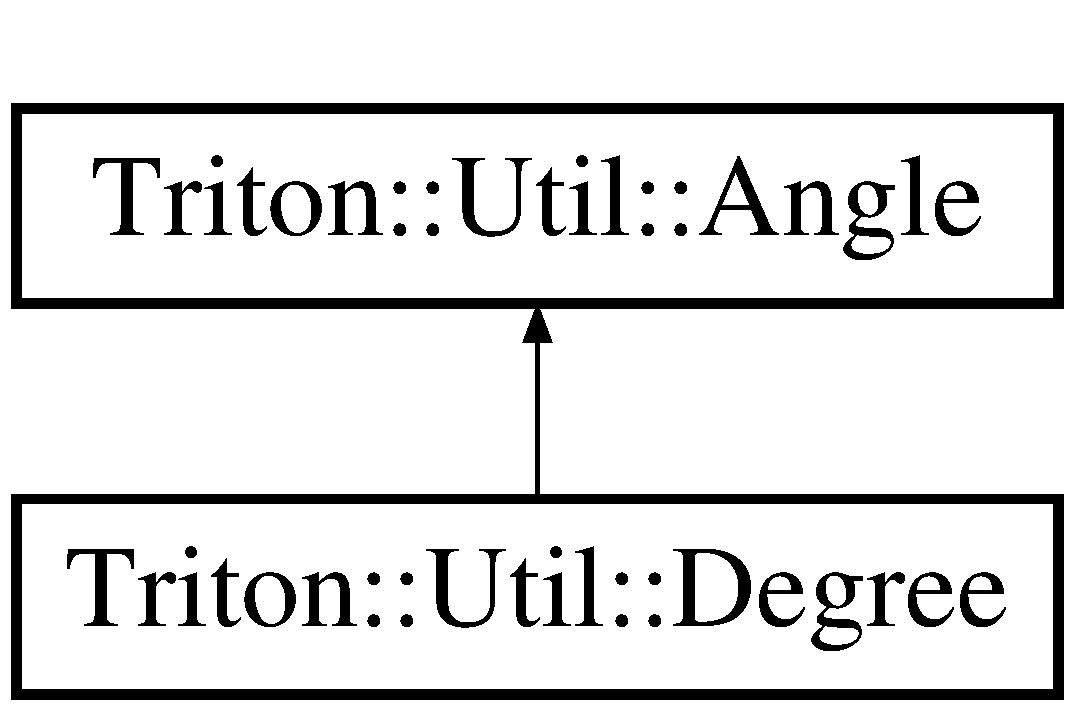
\includegraphics[height=2.000000cm]{struct_triton_1_1_util_1_1_degree}
\end{center}
\end{figure}
\subsection*{Public Member Functions}
\begin{DoxyCompactItemize}
\item 
\hyperlink{struct_triton_1_1_util_1_1_degree_a1775e5cc6bd96b15dbab56e2a6a6daf6}{Degree} (float \hyperlink{struct_triton_1_1_util_1_1_angle_af7d7f20a28c150b09776a35bc1dae0c4}{ang})
\item 
\hyperlink{struct_triton_1_1_util_1_1_degree_aa380efe33bd325c67dd08c3c73404901}{Degree} (const \hyperlink{struct_triton_1_1_util_1_1_radian}{Radian} \&rad)
\item 
\hyperlink{struct_triton_1_1_util_1_1_degree}{Degree} \& \hyperlink{struct_triton_1_1_util_1_1_degree_a74ad31a41cdc3ea6c0b6fdd3949a3411}{operator=} (const \hyperlink{struct_triton_1_1_util_1_1_radian}{Radian} \&rad)
\item 
\hyperlink{struct_triton_1_1_util_1_1_degree_aba55c9e80b400d129fda6596fdf26d5a}{operator Radian} ()
\item 
\hyperlink{struct_triton_1_1_util_1_1_radian}{Radian} \hyperlink{struct_triton_1_1_util_1_1_degree_ab1a544079c563045d5ddedae4ca52ca4}{To\+Radian} ()
\item 
Rotation\+Type \hyperlink{struct_triton_1_1_util_1_1_degree_a31e2a2094c705e9195c1e8f076aa690d}{Get\+Rotation\+Type} ()
\end{DoxyCompactItemize}
\subsection*{Additional Inherited Members}


\subsection{Detailed Description}
A simplistic \hyperlink{struct_triton_1_1_util_1_1_degree}{Degree} object. 

Based on \hyperlink{struct_triton_1_1_util_1_1_angle}{Angle} 

Definition at line 36 of file angle.\+h.



\subsection{Constructor \& Destructor Documentation}
\hypertarget{struct_triton_1_1_util_1_1_degree_a1775e5cc6bd96b15dbab56e2a6a6daf6}{}\index{Triton\+::\+Util\+::\+Degree@{Triton\+::\+Util\+::\+Degree}!Degree@{Degree}}
\index{Degree@{Degree}!Triton\+::\+Util\+::\+Degree@{Triton\+::\+Util\+::\+Degree}}
\subsubsection[{Degree}]{\setlength{\rightskip}{0pt plus 5cm}Triton\+::\+Util\+::\+Degree\+::\+Degree (
\begin{DoxyParamCaption}
\item[{float}]{ang}
\end{DoxyParamCaption}
)\hspace{0.3cm}{\ttfamily [inline]}}\label{struct_triton_1_1_util_1_1_degree_a1775e5cc6bd96b15dbab56e2a6a6daf6}


Definition at line 38 of file angle.\+h.

\hypertarget{struct_triton_1_1_util_1_1_degree_aa380efe33bd325c67dd08c3c73404901}{}\index{Triton\+::\+Util\+::\+Degree@{Triton\+::\+Util\+::\+Degree}!Degree@{Degree}}
\index{Degree@{Degree}!Triton\+::\+Util\+::\+Degree@{Triton\+::\+Util\+::\+Degree}}
\subsubsection[{Degree}]{\setlength{\rightskip}{0pt plus 5cm}Triton\+::\+Util\+::\+Degree\+::\+Degree (
\begin{DoxyParamCaption}
\item[{const {\bf Radian} \&}]{rad}
\end{DoxyParamCaption}
)}\label{struct_triton_1_1_util_1_1_degree_aa380efe33bd325c67dd08c3c73404901}


\subsection{Member Function Documentation}
\hypertarget{struct_triton_1_1_util_1_1_degree_a31e2a2094c705e9195c1e8f076aa690d}{}\index{Triton\+::\+Util\+::\+Degree@{Triton\+::\+Util\+::\+Degree}!Get\+Rotation\+Type@{Get\+Rotation\+Type}}
\index{Get\+Rotation\+Type@{Get\+Rotation\+Type}!Triton\+::\+Util\+::\+Degree@{Triton\+::\+Util\+::\+Degree}}
\subsubsection[{Get\+Rotation\+Type}]{\setlength{\rightskip}{0pt plus 5cm}Rotation\+Type Triton\+::\+Util\+::\+Degree\+::\+Get\+Rotation\+Type (
\begin{DoxyParamCaption}
{}
\end{DoxyParamCaption}
)\hspace{0.3cm}{\ttfamily [inline]}, {\ttfamily [virtual]}}\label{struct_triton_1_1_util_1_1_degree_a31e2a2094c705e9195c1e8f076aa690d}


Reimplemented from \hyperlink{struct_triton_1_1_util_1_1_angle_ac62cfbc48317457ff0992bc994f94f3e}{Triton\+::\+Util\+::\+Angle}.



Definition at line 46 of file angle.\+h.

\hypertarget{struct_triton_1_1_util_1_1_degree_aba55c9e80b400d129fda6596fdf26d5a}{}\index{Triton\+::\+Util\+::\+Degree@{Triton\+::\+Util\+::\+Degree}!operator Radian@{operator Radian}}
\index{operator Radian@{operator Radian}!Triton\+::\+Util\+::\+Degree@{Triton\+::\+Util\+::\+Degree}}
\subsubsection[{operator Radian}]{\setlength{\rightskip}{0pt plus 5cm}Triton\+::\+Util\+::\+Degree\+::operator {\bf Radian} (
\begin{DoxyParamCaption}
{}
\end{DoxyParamCaption}
)}\label{struct_triton_1_1_util_1_1_degree_aba55c9e80b400d129fda6596fdf26d5a}
\hypertarget{struct_triton_1_1_util_1_1_degree_a74ad31a41cdc3ea6c0b6fdd3949a3411}{}\index{Triton\+::\+Util\+::\+Degree@{Triton\+::\+Util\+::\+Degree}!operator=@{operator=}}
\index{operator=@{operator=}!Triton\+::\+Util\+::\+Degree@{Triton\+::\+Util\+::\+Degree}}
\subsubsection[{operator=}]{\setlength{\rightskip}{0pt plus 5cm}{\bf Degree}\& Triton\+::\+Util\+::\+Degree\+::operator= (
\begin{DoxyParamCaption}
\item[{const {\bf Radian} \&}]{rad}
\end{DoxyParamCaption}
)}\label{struct_triton_1_1_util_1_1_degree_a74ad31a41cdc3ea6c0b6fdd3949a3411}
\hypertarget{struct_triton_1_1_util_1_1_degree_ab1a544079c563045d5ddedae4ca52ca4}{}\index{Triton\+::\+Util\+::\+Degree@{Triton\+::\+Util\+::\+Degree}!To\+Radian@{To\+Radian}}
\index{To\+Radian@{To\+Radian}!Triton\+::\+Util\+::\+Degree@{Triton\+::\+Util\+::\+Degree}}
\subsubsection[{To\+Radian}]{\setlength{\rightskip}{0pt plus 5cm}{\bf Radian} Triton\+::\+Util\+::\+Degree\+::\+To\+Radian (
\begin{DoxyParamCaption}
{}
\end{DoxyParamCaption}
)}\label{struct_triton_1_1_util_1_1_degree_ab1a544079c563045d5ddedae4ca52ca4}


The documentation for this struct was generated from the following file\+:\begin{DoxyCompactItemize}
\item 
util/\hyperlink{angle_8h}{angle.\+h}\end{DoxyCompactItemize}

\hypertarget{class_tri_1_1_graphic_1_1_draw2_d}{}\section{Tri\+:\+:Graphic\+:\+:Draw2\+D Class Reference}
\label{class_tri_1_1_graphic_1_1_draw2_d}\index{Tri\+::\+Graphic\+::\+Draw2\+D@{Tri\+::\+Graphic\+::\+Draw2\+D}}


{\ttfamily \#include $<$render.\+h$>$}

Inheritance diagram for Tri\+:\+:Graphic\+:\+:Draw2\+D\+:\begin{figure}[H]
\begin{center}
\leavevmode
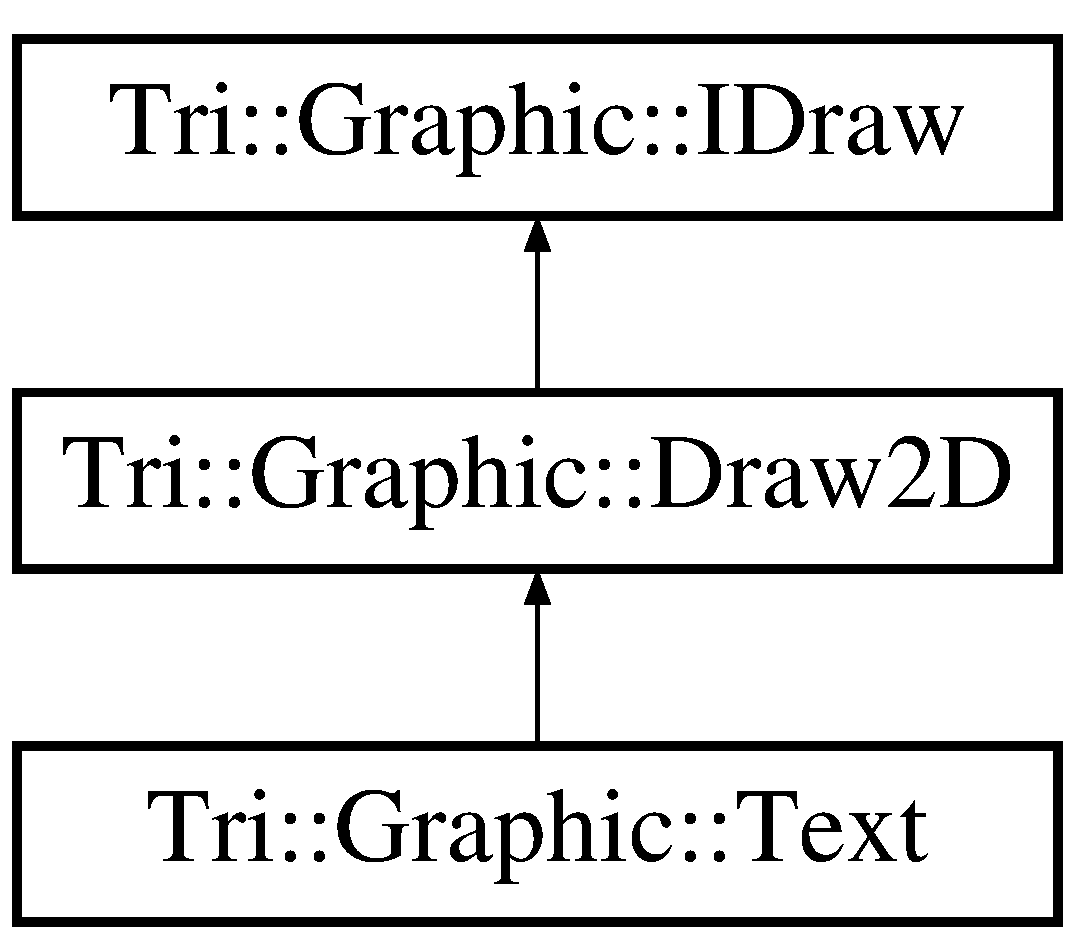
\includegraphics[height=3.000000cm]{class_tri_1_1_graphic_1_1_draw2_d}
\end{center}
\end{figure}
\subsection*{Public Member Functions}
\begin{DoxyCompactItemize}
\item 
\hyperlink{class_tri_1_1_graphic_1_1_draw2_d_a7a4fcef9fa0faa8e25ece699d28785c6}{Draw2\+D} (Resource\+::\+Image texture)
\item 
bool \hyperlink{class_tri_1_1_graphic_1_1_draw2_d_ade0b5fadee0bbfd97bbf1619cb16c6ea}{Assign\+Texture} (Resource\+::\+Image texture)
\item 
void \hyperlink{class_tri_1_1_graphic_1_1_draw2_d_ad0a6811ffd761114919f01b4dfcdc0d7}{Rotate} (Util\+::\+Vec2$<$ Angle $>$ rotation)
\item 
void \hyperlink{class_tri_1_1_graphic_1_1_draw2_d_a02434f6c9d46a00009afa18e9a2599f6}{Move\+To} (Util\+::\+Vec2$<$ double $>$ position)
\item 
void \hyperlink{class_tri_1_1_graphic_1_1_draw2_d_ae446a7a0c520d9cf2f358d63ead9e50f}{Rescale} (Util\+::\+Vec2$<$ float $>$ scale)
\item 
void \hyperlink{class_tri_1_1_graphic_1_1_draw2_d_aef4e47c193df3832c46a446745aeec0a}{Set\+Z\+Level} (double z)
\item 
Util\+::\+Vec2$<$ double $>$ \hyperlink{class_tri_1_1_graphic_1_1_draw2_d_a3e5faa6322d8f0743bd13efdd83ad4a9}{Get\+Position} ()
\item 
Util\+::\+Vec2$<$ Util\+::\+Radian $>$ \hyperlink{class_tri_1_1_graphic_1_1_draw2_d_a9b234a4abe1716e06dcbf1eea330dc3d}{Get\+Rotation} ()
\item 
Util\+::\+Vec2$<$ float $>$ \hyperlink{class_tri_1_1_graphic_1_1_draw2_d_a633dbe8143a7fcb6981be2447d782490}{Get\+Scale} ()
\item 
double \hyperlink{class_tri_1_1_graphic_1_1_draw2_d_a314b4296587449bda1f1bfe443909581}{Get\+Z\+Level} ()
\item 
\hyperlink{namespace_tri_1_1_graphic_a7b3538cdaff9bf96489c56a4f48a5f9a}{Mat4} \hyperlink{class_tri_1_1_graphic_1_1_draw2_d_ab9fda1624fd99c6ab7d05e8a9aa2b4bd}{Get\+Model\+Matrix} ()
\end{DoxyCompactItemize}
\subsection*{Protected Member Functions}
\begin{DoxyCompactItemize}
\item 
virtual void \hyperlink{class_tri_1_1_graphic_1_1_draw2_d_ab291c401ee1ec4d505665e8b2c1d21cc}{On\+Rotate} (Util\+::\+Vec2$<$ Angle $>$ \&r\+Rotation)
\item 
virtual void \hyperlink{class_tri_1_1_graphic_1_1_draw2_d_ab9b725d76f67e0edfb920ba5b44cf8d3}{On\+Move} (Util\+::\+Vec2$<$ double $>$ \&r\+Position)
\item 
virtual void \hyperlink{class_tri_1_1_graphic_1_1_draw2_d_a7494de2373e773b7380ddb66b1edafe8}{On\+Rescale} (Util\+::\+Vec2$<$ float $>$ \&r\+Scale)
\item 
virtual void \hyperlink{class_tri_1_1_graphic_1_1_draw2_d_a31a8a3b099dfe0ad23f4d7378846a731}{On\+Z\+Level\+Change} (double \&r\+Z\+Level)
\end{DoxyCompactItemize}
\subsection*{Additional Inherited Members}


\subsection{Detailed Description}


Definition at line 65 of file render.\+h.



\subsection{Constructor \& Destructor Documentation}
\hypertarget{class_tri_1_1_graphic_1_1_draw2_d_a7a4fcef9fa0faa8e25ece699d28785c6}{}\index{Tri\+::\+Graphic\+::\+Draw2\+D@{Tri\+::\+Graphic\+::\+Draw2\+D}!Draw2\+D@{Draw2\+D}}
\index{Draw2\+D@{Draw2\+D}!Tri\+::\+Graphic\+::\+Draw2\+D@{Tri\+::\+Graphic\+::\+Draw2\+D}}
\subsubsection[{Draw2\+D}]{\setlength{\rightskip}{0pt plus 5cm}Tri\+::\+Graphic\+::\+Draw2\+D\+::\+Draw2\+D (
\begin{DoxyParamCaption}
\item[{Resource\+::\+Image}]{texture}
\end{DoxyParamCaption}
)\hspace{0.3cm}{\ttfamily [inline]}}\label{class_tri_1_1_graphic_1_1_draw2_d_a7a4fcef9fa0faa8e25ece699d28785c6}


Definition at line 78 of file render.\+h.



\subsection{Member Function Documentation}
\hypertarget{class_tri_1_1_graphic_1_1_draw2_d_ade0b5fadee0bbfd97bbf1619cb16c6ea}{}\index{Tri\+::\+Graphic\+::\+Draw2\+D@{Tri\+::\+Graphic\+::\+Draw2\+D}!Assign\+Texture@{Assign\+Texture}}
\index{Assign\+Texture@{Assign\+Texture}!Tri\+::\+Graphic\+::\+Draw2\+D@{Tri\+::\+Graphic\+::\+Draw2\+D}}
\subsubsection[{Assign\+Texture}]{\setlength{\rightskip}{0pt plus 5cm}bool Tri\+::\+Graphic\+::\+Draw2\+D\+::\+Assign\+Texture (
\begin{DoxyParamCaption}
\item[{Resource\+::\+Image}]{texture}
\end{DoxyParamCaption}
)}\label{class_tri_1_1_graphic_1_1_draw2_d_ade0b5fadee0bbfd97bbf1619cb16c6ea}
\hypertarget{class_tri_1_1_graphic_1_1_draw2_d_ab9fda1624fd99c6ab7d05e8a9aa2b4bd}{}\index{Tri\+::\+Graphic\+::\+Draw2\+D@{Tri\+::\+Graphic\+::\+Draw2\+D}!Get\+Model\+Matrix@{Get\+Model\+Matrix}}
\index{Get\+Model\+Matrix@{Get\+Model\+Matrix}!Tri\+::\+Graphic\+::\+Draw2\+D@{Tri\+::\+Graphic\+::\+Draw2\+D}}
\subsubsection[{Get\+Model\+Matrix}]{\setlength{\rightskip}{0pt plus 5cm}{\bf Mat4} Tri\+::\+Graphic\+::\+Draw2\+D\+::\+Get\+Model\+Matrix (
\begin{DoxyParamCaption}
{}
\end{DoxyParamCaption}
)\hspace{0.3cm}{\ttfamily [virtual]}}\label{class_tri_1_1_graphic_1_1_draw2_d_ab9fda1624fd99c6ab7d05e8a9aa2b4bd}


Implements \hyperlink{class_tri_1_1_graphic_1_1_i_draw_ae6c6b2e08c6d6e2d4f8a07b24de0018c}{Tri\+::\+Graphic\+::\+I\+Draw}.

\hypertarget{class_tri_1_1_graphic_1_1_draw2_d_a3e5faa6322d8f0743bd13efdd83ad4a9}{}\index{Tri\+::\+Graphic\+::\+Draw2\+D@{Tri\+::\+Graphic\+::\+Draw2\+D}!Get\+Position@{Get\+Position}}
\index{Get\+Position@{Get\+Position}!Tri\+::\+Graphic\+::\+Draw2\+D@{Tri\+::\+Graphic\+::\+Draw2\+D}}
\subsubsection[{Get\+Position}]{\setlength{\rightskip}{0pt plus 5cm}Util\+::\+Vec2$<$double$>$ Tri\+::\+Graphic\+::\+Draw2\+D\+::\+Get\+Position (
\begin{DoxyParamCaption}
{}
\end{DoxyParamCaption}
)}\label{class_tri_1_1_graphic_1_1_draw2_d_a3e5faa6322d8f0743bd13efdd83ad4a9}
\hypertarget{class_tri_1_1_graphic_1_1_draw2_d_a9b234a4abe1716e06dcbf1eea330dc3d}{}\index{Tri\+::\+Graphic\+::\+Draw2\+D@{Tri\+::\+Graphic\+::\+Draw2\+D}!Get\+Rotation@{Get\+Rotation}}
\index{Get\+Rotation@{Get\+Rotation}!Tri\+::\+Graphic\+::\+Draw2\+D@{Tri\+::\+Graphic\+::\+Draw2\+D}}
\subsubsection[{Get\+Rotation}]{\setlength{\rightskip}{0pt plus 5cm}Util\+::\+Vec2$<$Util\+::\+Radian$>$ Tri\+::\+Graphic\+::\+Draw2\+D\+::\+Get\+Rotation (
\begin{DoxyParamCaption}
{}
\end{DoxyParamCaption}
)}\label{class_tri_1_1_graphic_1_1_draw2_d_a9b234a4abe1716e06dcbf1eea330dc3d}
\hypertarget{class_tri_1_1_graphic_1_1_draw2_d_a633dbe8143a7fcb6981be2447d782490}{}\index{Tri\+::\+Graphic\+::\+Draw2\+D@{Tri\+::\+Graphic\+::\+Draw2\+D}!Get\+Scale@{Get\+Scale}}
\index{Get\+Scale@{Get\+Scale}!Tri\+::\+Graphic\+::\+Draw2\+D@{Tri\+::\+Graphic\+::\+Draw2\+D}}
\subsubsection[{Get\+Scale}]{\setlength{\rightskip}{0pt plus 5cm}Util\+::\+Vec2$<$float$>$ Tri\+::\+Graphic\+::\+Draw2\+D\+::\+Get\+Scale (
\begin{DoxyParamCaption}
{}
\end{DoxyParamCaption}
)}\label{class_tri_1_1_graphic_1_1_draw2_d_a633dbe8143a7fcb6981be2447d782490}
\hypertarget{class_tri_1_1_graphic_1_1_draw2_d_a314b4296587449bda1f1bfe443909581}{}\index{Tri\+::\+Graphic\+::\+Draw2\+D@{Tri\+::\+Graphic\+::\+Draw2\+D}!Get\+Z\+Level@{Get\+Z\+Level}}
\index{Get\+Z\+Level@{Get\+Z\+Level}!Tri\+::\+Graphic\+::\+Draw2\+D@{Tri\+::\+Graphic\+::\+Draw2\+D}}
\subsubsection[{Get\+Z\+Level}]{\setlength{\rightskip}{0pt plus 5cm}double Tri\+::\+Graphic\+::\+Draw2\+D\+::\+Get\+Z\+Level (
\begin{DoxyParamCaption}
{}
\end{DoxyParamCaption}
)}\label{class_tri_1_1_graphic_1_1_draw2_d_a314b4296587449bda1f1bfe443909581}
\hypertarget{class_tri_1_1_graphic_1_1_draw2_d_a02434f6c9d46a00009afa18e9a2599f6}{}\index{Tri\+::\+Graphic\+::\+Draw2\+D@{Tri\+::\+Graphic\+::\+Draw2\+D}!Move\+To@{Move\+To}}
\index{Move\+To@{Move\+To}!Tri\+::\+Graphic\+::\+Draw2\+D@{Tri\+::\+Graphic\+::\+Draw2\+D}}
\subsubsection[{Move\+To}]{\setlength{\rightskip}{0pt plus 5cm}void Tri\+::\+Graphic\+::\+Draw2\+D\+::\+Move\+To (
\begin{DoxyParamCaption}
\item[{Util\+::\+Vec2$<$ double $>$}]{position}
\end{DoxyParamCaption}
)}\label{class_tri_1_1_graphic_1_1_draw2_d_a02434f6c9d46a00009afa18e9a2599f6}
\hypertarget{class_tri_1_1_graphic_1_1_draw2_d_ab9b725d76f67e0edfb920ba5b44cf8d3}{}\index{Tri\+::\+Graphic\+::\+Draw2\+D@{Tri\+::\+Graphic\+::\+Draw2\+D}!On\+Move@{On\+Move}}
\index{On\+Move@{On\+Move}!Tri\+::\+Graphic\+::\+Draw2\+D@{Tri\+::\+Graphic\+::\+Draw2\+D}}
\subsubsection[{On\+Move}]{\setlength{\rightskip}{0pt plus 5cm}virtual void Tri\+::\+Graphic\+::\+Draw2\+D\+::\+On\+Move (
\begin{DoxyParamCaption}
\item[{Util\+::\+Vec2$<$ double $>$ \&}]{r\+Position}
\end{DoxyParamCaption}
)\hspace{0.3cm}{\ttfamily [inline]}, {\ttfamily [protected]}, {\ttfamily [virtual]}}\label{class_tri_1_1_graphic_1_1_draw2_d_ab9b725d76f67e0edfb920ba5b44cf8d3}


Definition at line 74 of file render.\+h.

\hypertarget{class_tri_1_1_graphic_1_1_draw2_d_a7494de2373e773b7380ddb66b1edafe8}{}\index{Tri\+::\+Graphic\+::\+Draw2\+D@{Tri\+::\+Graphic\+::\+Draw2\+D}!On\+Rescale@{On\+Rescale}}
\index{On\+Rescale@{On\+Rescale}!Tri\+::\+Graphic\+::\+Draw2\+D@{Tri\+::\+Graphic\+::\+Draw2\+D}}
\subsubsection[{On\+Rescale}]{\setlength{\rightskip}{0pt plus 5cm}virtual void Tri\+::\+Graphic\+::\+Draw2\+D\+::\+On\+Rescale (
\begin{DoxyParamCaption}
\item[{Util\+::\+Vec2$<$ float $>$ \&}]{r\+Scale}
\end{DoxyParamCaption}
)\hspace{0.3cm}{\ttfamily [inline]}, {\ttfamily [protected]}, {\ttfamily [virtual]}}\label{class_tri_1_1_graphic_1_1_draw2_d_a7494de2373e773b7380ddb66b1edafe8}


Definition at line 75 of file render.\+h.

\hypertarget{class_tri_1_1_graphic_1_1_draw2_d_ab291c401ee1ec4d505665e8b2c1d21cc}{}\index{Tri\+::\+Graphic\+::\+Draw2\+D@{Tri\+::\+Graphic\+::\+Draw2\+D}!On\+Rotate@{On\+Rotate}}
\index{On\+Rotate@{On\+Rotate}!Tri\+::\+Graphic\+::\+Draw2\+D@{Tri\+::\+Graphic\+::\+Draw2\+D}}
\subsubsection[{On\+Rotate}]{\setlength{\rightskip}{0pt plus 5cm}virtual void Tri\+::\+Graphic\+::\+Draw2\+D\+::\+On\+Rotate (
\begin{DoxyParamCaption}
\item[{Util\+::\+Vec2$<$ Angle $>$ \&}]{r\+Rotation}
\end{DoxyParamCaption}
)\hspace{0.3cm}{\ttfamily [inline]}, {\ttfamily [protected]}, {\ttfamily [virtual]}}\label{class_tri_1_1_graphic_1_1_draw2_d_ab291c401ee1ec4d505665e8b2c1d21cc}


Definition at line 73 of file render.\+h.

\hypertarget{class_tri_1_1_graphic_1_1_draw2_d_a31a8a3b099dfe0ad23f4d7378846a731}{}\index{Tri\+::\+Graphic\+::\+Draw2\+D@{Tri\+::\+Graphic\+::\+Draw2\+D}!On\+Z\+Level\+Change@{On\+Z\+Level\+Change}}
\index{On\+Z\+Level\+Change@{On\+Z\+Level\+Change}!Tri\+::\+Graphic\+::\+Draw2\+D@{Tri\+::\+Graphic\+::\+Draw2\+D}}
\subsubsection[{On\+Z\+Level\+Change}]{\setlength{\rightskip}{0pt plus 5cm}virtual void Tri\+::\+Graphic\+::\+Draw2\+D\+::\+On\+Z\+Level\+Change (
\begin{DoxyParamCaption}
\item[{double \&}]{r\+Z\+Level}
\end{DoxyParamCaption}
)\hspace{0.3cm}{\ttfamily [inline]}, {\ttfamily [protected]}, {\ttfamily [virtual]}}\label{class_tri_1_1_graphic_1_1_draw2_d_a31a8a3b099dfe0ad23f4d7378846a731}


Definition at line 76 of file render.\+h.

\hypertarget{class_tri_1_1_graphic_1_1_draw2_d_ae446a7a0c520d9cf2f358d63ead9e50f}{}\index{Tri\+::\+Graphic\+::\+Draw2\+D@{Tri\+::\+Graphic\+::\+Draw2\+D}!Rescale@{Rescale}}
\index{Rescale@{Rescale}!Tri\+::\+Graphic\+::\+Draw2\+D@{Tri\+::\+Graphic\+::\+Draw2\+D}}
\subsubsection[{Rescale}]{\setlength{\rightskip}{0pt plus 5cm}void Tri\+::\+Graphic\+::\+Draw2\+D\+::\+Rescale (
\begin{DoxyParamCaption}
\item[{Util\+::\+Vec2$<$ float $>$}]{scale}
\end{DoxyParamCaption}
)}\label{class_tri_1_1_graphic_1_1_draw2_d_ae446a7a0c520d9cf2f358d63ead9e50f}
\hypertarget{class_tri_1_1_graphic_1_1_draw2_d_ad0a6811ffd761114919f01b4dfcdc0d7}{}\index{Tri\+::\+Graphic\+::\+Draw2\+D@{Tri\+::\+Graphic\+::\+Draw2\+D}!Rotate@{Rotate}}
\index{Rotate@{Rotate}!Tri\+::\+Graphic\+::\+Draw2\+D@{Tri\+::\+Graphic\+::\+Draw2\+D}}
\subsubsection[{Rotate}]{\setlength{\rightskip}{0pt plus 5cm}void Tri\+::\+Graphic\+::\+Draw2\+D\+::\+Rotate (
\begin{DoxyParamCaption}
\item[{Util\+::\+Vec2$<$ Angle $>$}]{rotation}
\end{DoxyParamCaption}
)}\label{class_tri_1_1_graphic_1_1_draw2_d_ad0a6811ffd761114919f01b4dfcdc0d7}
\hypertarget{class_tri_1_1_graphic_1_1_draw2_d_aef4e47c193df3832c46a446745aeec0a}{}\index{Tri\+::\+Graphic\+::\+Draw2\+D@{Tri\+::\+Graphic\+::\+Draw2\+D}!Set\+Z\+Level@{Set\+Z\+Level}}
\index{Set\+Z\+Level@{Set\+Z\+Level}!Tri\+::\+Graphic\+::\+Draw2\+D@{Tri\+::\+Graphic\+::\+Draw2\+D}}
\subsubsection[{Set\+Z\+Level}]{\setlength{\rightskip}{0pt plus 5cm}void Tri\+::\+Graphic\+::\+Draw2\+D\+::\+Set\+Z\+Level (
\begin{DoxyParamCaption}
\item[{double}]{z}
\end{DoxyParamCaption}
)}\label{class_tri_1_1_graphic_1_1_draw2_d_aef4e47c193df3832c46a446745aeec0a}


The documentation for this class was generated from the following file\+:\begin{DoxyCompactItemize}
\item 
graphic/\hyperlink{render_8h}{render.\+h}\end{DoxyCompactItemize}

\hypertarget{class_tri_1_1_graphic_1_1_draw3_d}{}\section{Tri\+:\+:Graphic\+:\+:Draw3\+D Class Reference}
\label{class_tri_1_1_graphic_1_1_draw3_d}\index{Tri\+::\+Graphic\+::\+Draw3\+D@{Tri\+::\+Graphic\+::\+Draw3\+D}}


{\ttfamily \#include $<$render.\+h$>$}

Inheritance diagram for Tri\+:\+:Graphic\+:\+:Draw3\+D\+:\begin{figure}[H]
\begin{center}
\leavevmode
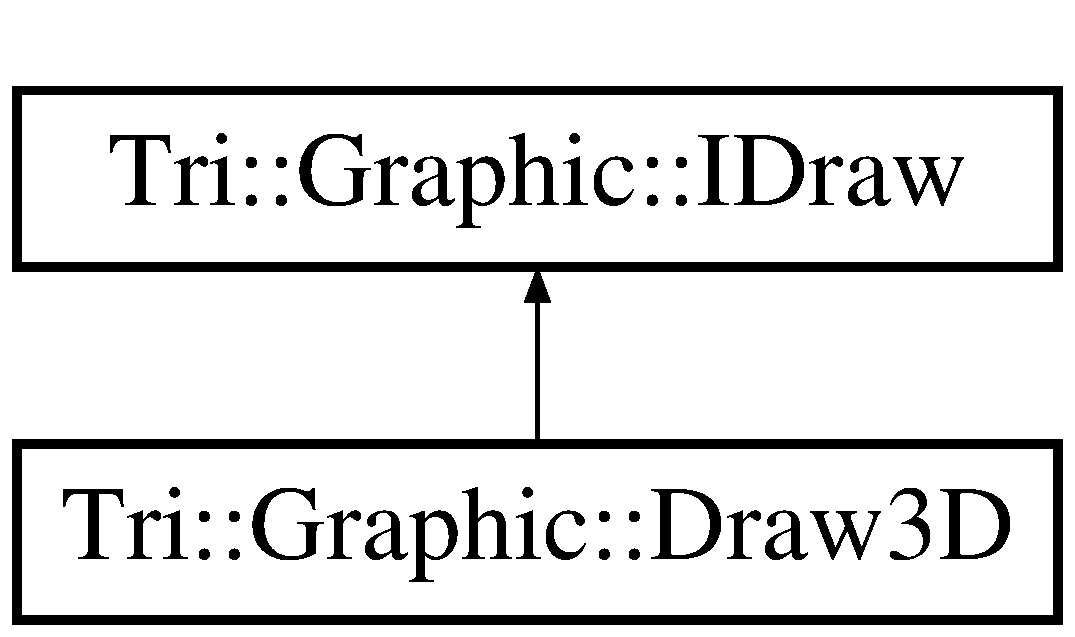
\includegraphics[height=2.000000cm]{class_tri_1_1_graphic_1_1_draw3_d}
\end{center}
\end{figure}
\subsection*{Public Member Functions}
\begin{DoxyCompactItemize}
\item 
\hyperlink{class_tri_1_1_graphic_1_1_draw3_d_a484cb66283010d4753461707fa0cbee0}{Draw3\+D} (Resource\+::\+Image texture, Resource\+::\+Model model)
\item 
bool \hyperlink{class_tri_1_1_graphic_1_1_draw3_d_a0a51e5e9ce64c32fd34572bca25151d8}{Assign\+Texture} (Resource\+::\+Image texture)
\item 
bool \hyperlink{class_tri_1_1_graphic_1_1_draw3_d_a7a8cad2d1fe74bb22dec83257ee6dba8}{Assign\+Model} (Resource\+::\+Model model)
\item 
void \hyperlink{class_tri_1_1_graphic_1_1_draw3_d_a2918187361ba98fe0495526e3f6d7637}{Rotate} (Util\+::\+Vec3$<$ Angle $>$ rotation)
\item 
void \hyperlink{class_tri_1_1_graphic_1_1_draw3_d_a72b1738a37ee3103794293baa513cdfb}{Move\+To} (Util\+::\+Vec3$<$ double $>$ position)
\item 
void \hyperlink{class_tri_1_1_graphic_1_1_draw3_d_a6b1edf2afb23174b24f4896f1596b848}{Rescale} (Util\+::\+Vec3$<$ float $>$ scale)
\item 
Util\+::\+Vec3$<$ double $>$ \hyperlink{class_tri_1_1_graphic_1_1_draw3_d_a893a85143357d9e0635cee5ec0ce33ea}{Get\+Position} ()
\item 
Util\+::\+Vec3$<$ Util\+::\+Radian $>$ \hyperlink{class_tri_1_1_graphic_1_1_draw3_d_a0bed6e0fc43eedd53e1624c62d5e6a0d}{Get\+Rotation} ()
\item 
Util\+::\+Vec3$<$ float $>$ \hyperlink{class_tri_1_1_graphic_1_1_draw3_d_a0ecf83003607b789ab22613ccc5651cc}{Get\+Scale} ()
\item 
\hyperlink{namespace_tri_1_1_graphic_a7b3538cdaff9bf96489c56a4f48a5f9a}{Mat4} \hyperlink{class_tri_1_1_graphic_1_1_draw3_d_a32ab7b7f0f956c0058a4a24a20ff4efc}{Get\+Model\+Matrix} ()
\end{DoxyCompactItemize}
\subsection*{Protected Member Functions}
\begin{DoxyCompactItemize}
\item 
virtual void \hyperlink{class_tri_1_1_graphic_1_1_draw3_d_a57889cd2622cc96fe924f6e5c890dcfb}{on\+Rotate} (Util\+::\+Vec3$<$ Angle $>$ \&r\+Rotations)
\item 
virtual void \hyperlink{class_tri_1_1_graphic_1_1_draw3_d_af5aaac36ec4674988d33189be6f2d2b0}{on\+Move} (Util\+::\+Vec3$<$ double $>$ \&r\+Position)
\item 
virtual void \hyperlink{class_tri_1_1_graphic_1_1_draw3_d_a77629dcfb43aa7a1487a104dfa550073}{on\+Rescale} (Util\+::\+Vec3$<$ float $>$ \&r\+Scale)
\end{DoxyCompactItemize}
\subsection*{Additional Inherited Members}


\subsection{Detailed Description}


Definition at line 94 of file render.\+h.



\subsection{Constructor \& Destructor Documentation}
\hypertarget{class_tri_1_1_graphic_1_1_draw3_d_a484cb66283010d4753461707fa0cbee0}{}\index{Tri\+::\+Graphic\+::\+Draw3\+D@{Tri\+::\+Graphic\+::\+Draw3\+D}!Draw3\+D@{Draw3\+D}}
\index{Draw3\+D@{Draw3\+D}!Tri\+::\+Graphic\+::\+Draw3\+D@{Tri\+::\+Graphic\+::\+Draw3\+D}}
\subsubsection[{Draw3\+D}]{\setlength{\rightskip}{0pt plus 5cm}Tri\+::\+Graphic\+::\+Draw3\+D\+::\+Draw3\+D (
\begin{DoxyParamCaption}
\item[{Resource\+::\+Image}]{texture, }
\item[{Resource\+::\+Model}]{model}
\end{DoxyParamCaption}
)\hspace{0.3cm}{\ttfamily [inline]}}\label{class_tri_1_1_graphic_1_1_draw3_d_a484cb66283010d4753461707fa0cbee0}


Definition at line 106 of file render.\+h.



\subsection{Member Function Documentation}
\hypertarget{class_tri_1_1_graphic_1_1_draw3_d_a7a8cad2d1fe74bb22dec83257ee6dba8}{}\index{Tri\+::\+Graphic\+::\+Draw3\+D@{Tri\+::\+Graphic\+::\+Draw3\+D}!Assign\+Model@{Assign\+Model}}
\index{Assign\+Model@{Assign\+Model}!Tri\+::\+Graphic\+::\+Draw3\+D@{Tri\+::\+Graphic\+::\+Draw3\+D}}
\subsubsection[{Assign\+Model}]{\setlength{\rightskip}{0pt plus 5cm}bool Tri\+::\+Graphic\+::\+Draw3\+D\+::\+Assign\+Model (
\begin{DoxyParamCaption}
\item[{Resource\+::\+Model}]{model}
\end{DoxyParamCaption}
)}\label{class_tri_1_1_graphic_1_1_draw3_d_a7a8cad2d1fe74bb22dec83257ee6dba8}
\hypertarget{class_tri_1_1_graphic_1_1_draw3_d_a0a51e5e9ce64c32fd34572bca25151d8}{}\index{Tri\+::\+Graphic\+::\+Draw3\+D@{Tri\+::\+Graphic\+::\+Draw3\+D}!Assign\+Texture@{Assign\+Texture}}
\index{Assign\+Texture@{Assign\+Texture}!Tri\+::\+Graphic\+::\+Draw3\+D@{Tri\+::\+Graphic\+::\+Draw3\+D}}
\subsubsection[{Assign\+Texture}]{\setlength{\rightskip}{0pt plus 5cm}bool Tri\+::\+Graphic\+::\+Draw3\+D\+::\+Assign\+Texture (
\begin{DoxyParamCaption}
\item[{Resource\+::\+Image}]{texture}
\end{DoxyParamCaption}
)}\label{class_tri_1_1_graphic_1_1_draw3_d_a0a51e5e9ce64c32fd34572bca25151d8}
\hypertarget{class_tri_1_1_graphic_1_1_draw3_d_a32ab7b7f0f956c0058a4a24a20ff4efc}{}\index{Tri\+::\+Graphic\+::\+Draw3\+D@{Tri\+::\+Graphic\+::\+Draw3\+D}!Get\+Model\+Matrix@{Get\+Model\+Matrix}}
\index{Get\+Model\+Matrix@{Get\+Model\+Matrix}!Tri\+::\+Graphic\+::\+Draw3\+D@{Tri\+::\+Graphic\+::\+Draw3\+D}}
\subsubsection[{Get\+Model\+Matrix}]{\setlength{\rightskip}{0pt plus 5cm}{\bf Mat4} Tri\+::\+Graphic\+::\+Draw3\+D\+::\+Get\+Model\+Matrix (
\begin{DoxyParamCaption}
{}
\end{DoxyParamCaption}
)\hspace{0.3cm}{\ttfamily [virtual]}}\label{class_tri_1_1_graphic_1_1_draw3_d_a32ab7b7f0f956c0058a4a24a20ff4efc}


Implements \hyperlink{class_tri_1_1_graphic_1_1_i_draw_ae6c6b2e08c6d6e2d4f8a07b24de0018c}{Tri\+::\+Graphic\+::\+I\+Draw}.

\hypertarget{class_tri_1_1_graphic_1_1_draw3_d_a893a85143357d9e0635cee5ec0ce33ea}{}\index{Tri\+::\+Graphic\+::\+Draw3\+D@{Tri\+::\+Graphic\+::\+Draw3\+D}!Get\+Position@{Get\+Position}}
\index{Get\+Position@{Get\+Position}!Tri\+::\+Graphic\+::\+Draw3\+D@{Tri\+::\+Graphic\+::\+Draw3\+D}}
\subsubsection[{Get\+Position}]{\setlength{\rightskip}{0pt plus 5cm}Util\+::\+Vec3$<$double$>$ Tri\+::\+Graphic\+::\+Draw3\+D\+::\+Get\+Position (
\begin{DoxyParamCaption}
{}
\end{DoxyParamCaption}
)}\label{class_tri_1_1_graphic_1_1_draw3_d_a893a85143357d9e0635cee5ec0ce33ea}
\hypertarget{class_tri_1_1_graphic_1_1_draw3_d_a0bed6e0fc43eedd53e1624c62d5e6a0d}{}\index{Tri\+::\+Graphic\+::\+Draw3\+D@{Tri\+::\+Graphic\+::\+Draw3\+D}!Get\+Rotation@{Get\+Rotation}}
\index{Get\+Rotation@{Get\+Rotation}!Tri\+::\+Graphic\+::\+Draw3\+D@{Tri\+::\+Graphic\+::\+Draw3\+D}}
\subsubsection[{Get\+Rotation}]{\setlength{\rightskip}{0pt plus 5cm}Util\+::\+Vec3$<$Util\+::\+Radian$>$ Tri\+::\+Graphic\+::\+Draw3\+D\+::\+Get\+Rotation (
\begin{DoxyParamCaption}
{}
\end{DoxyParamCaption}
)}\label{class_tri_1_1_graphic_1_1_draw3_d_a0bed6e0fc43eedd53e1624c62d5e6a0d}
\hypertarget{class_tri_1_1_graphic_1_1_draw3_d_a0ecf83003607b789ab22613ccc5651cc}{}\index{Tri\+::\+Graphic\+::\+Draw3\+D@{Tri\+::\+Graphic\+::\+Draw3\+D}!Get\+Scale@{Get\+Scale}}
\index{Get\+Scale@{Get\+Scale}!Tri\+::\+Graphic\+::\+Draw3\+D@{Tri\+::\+Graphic\+::\+Draw3\+D}}
\subsubsection[{Get\+Scale}]{\setlength{\rightskip}{0pt plus 5cm}Util\+::\+Vec3$<$float$>$ Tri\+::\+Graphic\+::\+Draw3\+D\+::\+Get\+Scale (
\begin{DoxyParamCaption}
{}
\end{DoxyParamCaption}
)}\label{class_tri_1_1_graphic_1_1_draw3_d_a0ecf83003607b789ab22613ccc5651cc}
\hypertarget{class_tri_1_1_graphic_1_1_draw3_d_a72b1738a37ee3103794293baa513cdfb}{}\index{Tri\+::\+Graphic\+::\+Draw3\+D@{Tri\+::\+Graphic\+::\+Draw3\+D}!Move\+To@{Move\+To}}
\index{Move\+To@{Move\+To}!Tri\+::\+Graphic\+::\+Draw3\+D@{Tri\+::\+Graphic\+::\+Draw3\+D}}
\subsubsection[{Move\+To}]{\setlength{\rightskip}{0pt plus 5cm}void Tri\+::\+Graphic\+::\+Draw3\+D\+::\+Move\+To (
\begin{DoxyParamCaption}
\item[{Util\+::\+Vec3$<$ double $>$}]{position}
\end{DoxyParamCaption}
)}\label{class_tri_1_1_graphic_1_1_draw3_d_a72b1738a37ee3103794293baa513cdfb}
\hypertarget{class_tri_1_1_graphic_1_1_draw3_d_af5aaac36ec4674988d33189be6f2d2b0}{}\index{Tri\+::\+Graphic\+::\+Draw3\+D@{Tri\+::\+Graphic\+::\+Draw3\+D}!on\+Move@{on\+Move}}
\index{on\+Move@{on\+Move}!Tri\+::\+Graphic\+::\+Draw3\+D@{Tri\+::\+Graphic\+::\+Draw3\+D}}
\subsubsection[{on\+Move}]{\setlength{\rightskip}{0pt plus 5cm}virtual void Tri\+::\+Graphic\+::\+Draw3\+D\+::on\+Move (
\begin{DoxyParamCaption}
\item[{Util\+::\+Vec3$<$ double $>$ \&}]{r\+Position}
\end{DoxyParamCaption}
)\hspace{0.3cm}{\ttfamily [inline]}, {\ttfamily [protected]}, {\ttfamily [virtual]}}\label{class_tri_1_1_graphic_1_1_draw3_d_af5aaac36ec4674988d33189be6f2d2b0}


Definition at line 103 of file render.\+h.

\hypertarget{class_tri_1_1_graphic_1_1_draw3_d_a77629dcfb43aa7a1487a104dfa550073}{}\index{Tri\+::\+Graphic\+::\+Draw3\+D@{Tri\+::\+Graphic\+::\+Draw3\+D}!on\+Rescale@{on\+Rescale}}
\index{on\+Rescale@{on\+Rescale}!Tri\+::\+Graphic\+::\+Draw3\+D@{Tri\+::\+Graphic\+::\+Draw3\+D}}
\subsubsection[{on\+Rescale}]{\setlength{\rightskip}{0pt plus 5cm}virtual void Tri\+::\+Graphic\+::\+Draw3\+D\+::on\+Rescale (
\begin{DoxyParamCaption}
\item[{Util\+::\+Vec3$<$ float $>$ \&}]{r\+Scale}
\end{DoxyParamCaption}
)\hspace{0.3cm}{\ttfamily [inline]}, {\ttfamily [protected]}, {\ttfamily [virtual]}}\label{class_tri_1_1_graphic_1_1_draw3_d_a77629dcfb43aa7a1487a104dfa550073}


Definition at line 104 of file render.\+h.

\hypertarget{class_tri_1_1_graphic_1_1_draw3_d_a57889cd2622cc96fe924f6e5c890dcfb}{}\index{Tri\+::\+Graphic\+::\+Draw3\+D@{Tri\+::\+Graphic\+::\+Draw3\+D}!on\+Rotate@{on\+Rotate}}
\index{on\+Rotate@{on\+Rotate}!Tri\+::\+Graphic\+::\+Draw3\+D@{Tri\+::\+Graphic\+::\+Draw3\+D}}
\subsubsection[{on\+Rotate}]{\setlength{\rightskip}{0pt plus 5cm}virtual void Tri\+::\+Graphic\+::\+Draw3\+D\+::on\+Rotate (
\begin{DoxyParamCaption}
\item[{Util\+::\+Vec3$<$ Angle $>$ \&}]{r\+Rotations}
\end{DoxyParamCaption}
)\hspace{0.3cm}{\ttfamily [inline]}, {\ttfamily [protected]}, {\ttfamily [virtual]}}\label{class_tri_1_1_graphic_1_1_draw3_d_a57889cd2622cc96fe924f6e5c890dcfb}


Definition at line 102 of file render.\+h.

\hypertarget{class_tri_1_1_graphic_1_1_draw3_d_a6b1edf2afb23174b24f4896f1596b848}{}\index{Tri\+::\+Graphic\+::\+Draw3\+D@{Tri\+::\+Graphic\+::\+Draw3\+D}!Rescale@{Rescale}}
\index{Rescale@{Rescale}!Tri\+::\+Graphic\+::\+Draw3\+D@{Tri\+::\+Graphic\+::\+Draw3\+D}}
\subsubsection[{Rescale}]{\setlength{\rightskip}{0pt plus 5cm}void Tri\+::\+Graphic\+::\+Draw3\+D\+::\+Rescale (
\begin{DoxyParamCaption}
\item[{Util\+::\+Vec3$<$ float $>$}]{scale}
\end{DoxyParamCaption}
)}\label{class_tri_1_1_graphic_1_1_draw3_d_a6b1edf2afb23174b24f4896f1596b848}
\hypertarget{class_tri_1_1_graphic_1_1_draw3_d_a2918187361ba98fe0495526e3f6d7637}{}\index{Tri\+::\+Graphic\+::\+Draw3\+D@{Tri\+::\+Graphic\+::\+Draw3\+D}!Rotate@{Rotate}}
\index{Rotate@{Rotate}!Tri\+::\+Graphic\+::\+Draw3\+D@{Tri\+::\+Graphic\+::\+Draw3\+D}}
\subsubsection[{Rotate}]{\setlength{\rightskip}{0pt plus 5cm}void Tri\+::\+Graphic\+::\+Draw3\+D\+::\+Rotate (
\begin{DoxyParamCaption}
\item[{Util\+::\+Vec3$<$ Angle $>$}]{rotation}
\end{DoxyParamCaption}
)}\label{class_tri_1_1_graphic_1_1_draw3_d_a2918187361ba98fe0495526e3f6d7637}


The documentation for this class was generated from the following file\+:\begin{DoxyCompactItemize}
\item 
graphic/\hyperlink{render_8h}{render.\+h}\end{DoxyCompactItemize}

\hypertarget{class_triton_1_1_util_1_1_dyn_array}{}\section{Triton\+:\+:Util\+:\+:Dyn\+Array$<$ T, Alloc $>$ Class Template Reference}
\label{class_triton_1_1_util_1_1_dyn_array}\index{Triton\+::\+Util\+::\+Dyn\+Array$<$ T, Alloc $>$@{Triton\+::\+Util\+::\+Dyn\+Array$<$ T, Alloc $>$}}


A standard C++ vector for better clarification and short hand of vectors.  




{\ttfamily \#include $<$util.\+h$>$}

Inheritance diagram for Triton\+:\+:Util\+:\+:Dyn\+Array$<$ T, Alloc $>$\+:\begin{figure}[H]
\begin{center}
\leavevmode
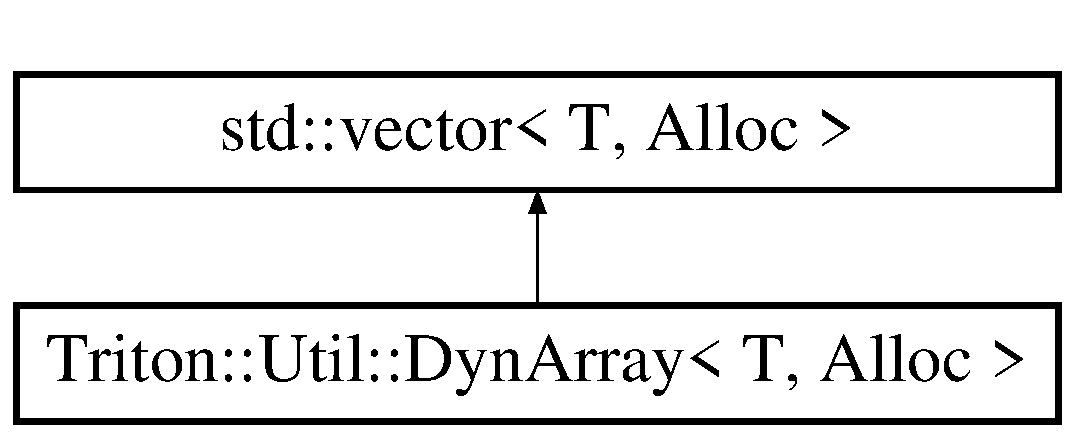
\includegraphics[height=2.000000cm]{class_triton_1_1_util_1_1_dyn_array}
\end{center}
\end{figure}


\subsection{Detailed Description}
\subsubsection*{template$<$typename T, class Alloc = std\+::allocator$<$\+T$>$$>$class Triton\+::\+Util\+::\+Dyn\+Array$<$ T, Alloc $>$}

A standard C++ vector for better clarification and short hand of vectors. 

Definition at line 111 of file util.\+h.



The documentation for this class was generated from the following file\+:\begin{DoxyCompactItemize}
\item 
util/\hyperlink{util_2util_8h}{util.\+h}\end{DoxyCompactItemize}

\hypertarget{class_triton_1_1_util_1_1_error}{}\section{Triton\+:\+:Util\+:\+:Error Class Reference}
\label{class_triton_1_1_util_1_1_error}\index{Triton\+::\+Util\+::\+Error@{Triton\+::\+Util\+::\+Error}}


An error based off \hyperlink{class_triton_1_1_util_1_1_exception}{Exception} for better clarification.  




{\ttfamily \#include $<$Exception.\+hpp$>$}

Inheritance diagram for Triton\+:\+:Util\+:\+:Error\+:\begin{figure}[H]
\begin{center}
\leavevmode
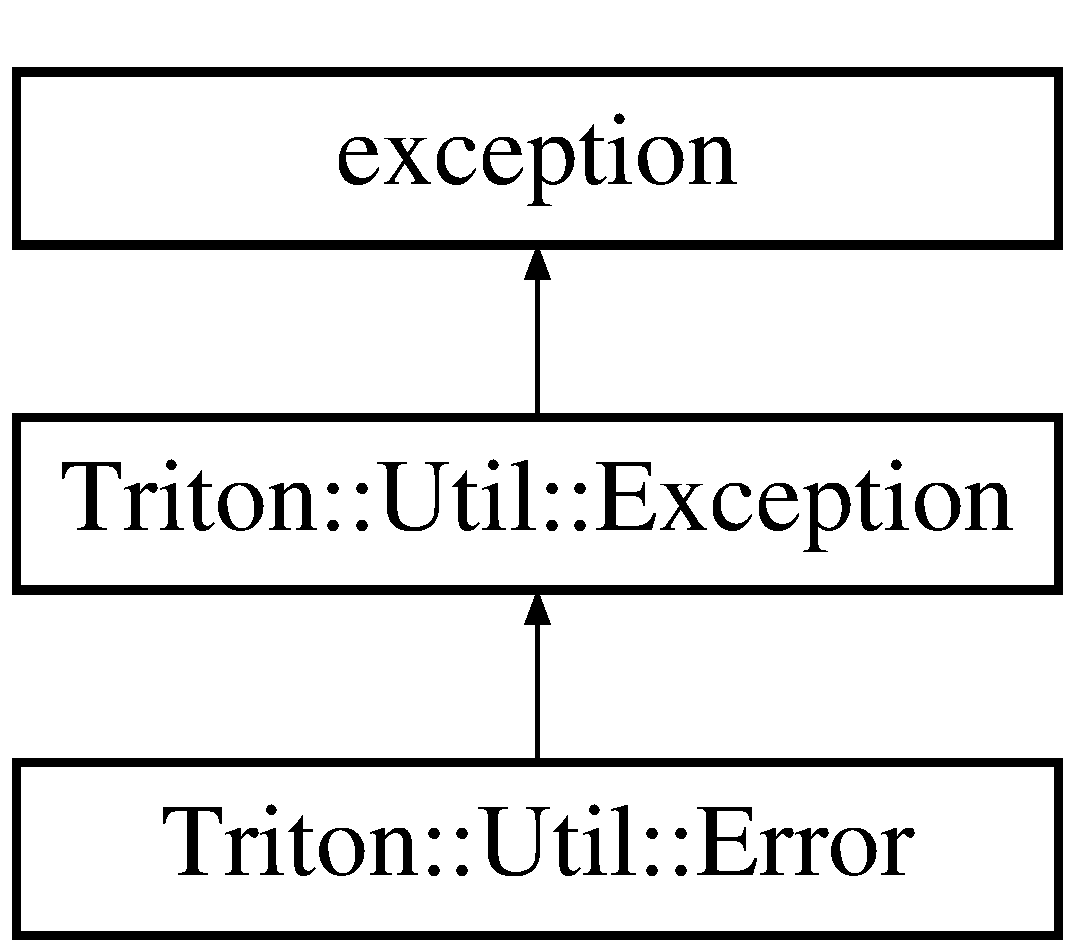
\includegraphics[height=3.000000cm]{class_triton_1_1_util_1_1_error}
\end{center}
\end{figure}
\subsection*{Public Member Functions}
\begin{DoxyCompactItemize}
\item 
\hyperlink{class_triton_1_1_util_1_1_error_a30e30a2532494d24964293e8ef664d32}{Error} (int error\+Code, \hyperlink{namespace_triton_1_1_util_a7e55ae91d6ccf98a52870cf7b7648eb7}{Exception\+String} error)
\item 
int \hyperlink{class_triton_1_1_util_1_1_error_ab72ec1bb13ec5e722542e82f0dbc553d}{Get\+Error\+Code} ()
\begin{DoxyCompactList}\small\item\em Returns the error\textquotesingle{}s code via stringstreams. \end{DoxyCompactList}\item 
\hyperlink{namespace_triton_1_1_util_a7e55ae91d6ccf98a52870cf7b7648eb7}{Exception\+String} \hyperlink{class_triton_1_1_util_1_1_error_a4d00634dc399c620eac99dc2c4ba5d3c}{Get\+Error\+Message} ()
\begin{DoxyCompactList}\small\item\em Returns the error\textquotesingle{}s readable statement. \end{DoxyCompactList}\end{DoxyCompactItemize}
\subsection*{Additional Inherited Members}


\subsection{Detailed Description}
An error based off \hyperlink{class_triton_1_1_util_1_1_exception}{Exception} for better clarification. 

Definition at line 51 of file Exception.\+hpp.



\subsection{Constructor \& Destructor Documentation}
\hypertarget{class_triton_1_1_util_1_1_error_a30e30a2532494d24964293e8ef664d32}{}\index{Triton\+::\+Util\+::\+Error@{Triton\+::\+Util\+::\+Error}!Error@{Error}}
\index{Error@{Error}!Triton\+::\+Util\+::\+Error@{Triton\+::\+Util\+::\+Error}}
\subsubsection[{Error}]{\setlength{\rightskip}{0pt plus 5cm}Triton\+::\+Util\+::\+Error\+::\+Error (
\begin{DoxyParamCaption}
\item[{int}]{error\+Code, }
\item[{{\bf Exception\+String}}]{error}
\end{DoxyParamCaption}
)\hspace{0.3cm}{\ttfamily [inline]}}\label{class_triton_1_1_util_1_1_error_a30e30a2532494d24964293e8ef664d32}
The constructor for \hyperlink{class_triton_1_1_util_1_1_error}{Error}


\begin{DoxyParams}{Parameters}
{\em error\+Code} & The error code to be applied to this exception \\
\hline
{\em error} & The error message of \hyperlink{class_triton_1_1_util_1_1_error}{Error} \\
\hline
\end{DoxyParams}


Definition at line 59 of file Exception.\+hpp.



\subsection{Member Function Documentation}
\hypertarget{class_triton_1_1_util_1_1_error_ab72ec1bb13ec5e722542e82f0dbc553d}{}\index{Triton\+::\+Util\+::\+Error@{Triton\+::\+Util\+::\+Error}!Get\+Error\+Code@{Get\+Error\+Code}}
\index{Get\+Error\+Code@{Get\+Error\+Code}!Triton\+::\+Util\+::\+Error@{Triton\+::\+Util\+::\+Error}}
\subsubsection[{Get\+Error\+Code}]{\setlength{\rightskip}{0pt plus 5cm}int Triton\+::\+Util\+::\+Error\+::\+Get\+Error\+Code (
\begin{DoxyParamCaption}
{}
\end{DoxyParamCaption}
)}\label{class_triton_1_1_util_1_1_error_ab72ec1bb13ec5e722542e82f0dbc553d}


Returns the error\textquotesingle{}s code via stringstreams. 

\hypertarget{class_triton_1_1_util_1_1_error_a4d00634dc399c620eac99dc2c4ba5d3c}{}\index{Triton\+::\+Util\+::\+Error@{Triton\+::\+Util\+::\+Error}!Get\+Error\+Message@{Get\+Error\+Message}}
\index{Get\+Error\+Message@{Get\+Error\+Message}!Triton\+::\+Util\+::\+Error@{Triton\+::\+Util\+::\+Error}}
\subsubsection[{Get\+Error\+Message}]{\setlength{\rightskip}{0pt plus 5cm}{\bf Exception\+String} Triton\+::\+Util\+::\+Error\+::\+Get\+Error\+Message (
\begin{DoxyParamCaption}
{}
\end{DoxyParamCaption}
)}\label{class_triton_1_1_util_1_1_error_a4d00634dc399c620eac99dc2c4ba5d3c}


Returns the error\textquotesingle{}s readable statement. 



The documentation for this class was generated from the following file\+:\begin{DoxyCompactItemize}
\item 
util/\+Exception/\hyperlink{_exception_8hpp}{Exception.\+hpp}\end{DoxyCompactItemize}

\hypertarget{class_triton_1_1_util_1_1_e_string}{}\section{Triton\+:\+:Util\+:\+:E\+String Class Reference}
\label{class_triton_1_1_util_1_1_e_string}\index{Triton\+::\+Util\+::\+E\+String@{Triton\+::\+Util\+::\+E\+String}}


Utility string class which is made to use in exceptions.  




{\ttfamily \#include $<$E\+String.\+hpp$>$}

\subsection*{Public Member Functions}
\begin{DoxyCompactItemize}
\item 
{\footnotesize template$<$typename str\+\_\+t $>$ }\\\hyperlink{class_triton_1_1_util_1_1_e_string_acad169bceb9c61936647d1c98b73329b}{E\+String} (str\+\_\+t string= \textquotesingle{}\textquotesingle{})
\begin{DoxyCompactList}\small\item\em The template constructor that works with all standard strings, can be used as default constructor. \end{DoxyCompactList}\item 
const char $\ast$ \hyperlink{class_triton_1_1_util_1_1_e_string_aabfcad680e8bf14100ad54f242a8b9bc}{c\+\_\+str} () const 
\begin{DoxyCompactList}\small\item\em Returns the cstring pointer, based on std\+::string\+::c\+\_\+str() \end{DoxyCompactList}\item 
size\+\_\+t \hyperlink{class_triton_1_1_util_1_1_e_string_a7108f6bdd705012da00fead8fff6181d}{size} ()
\begin{DoxyCompactList}\small\item\em Returns the length, based on std\+::string\+::c\+\_\+str() \end{DoxyCompactList}\item 
size\+\_\+t \hyperlink{class_triton_1_1_util_1_1_e_string_a917f720139bec99a944f42fb1c64c42b}{length} ()
\begin{DoxyCompactList}\small\item\em Returns the length, based on std\+::string\+::c\+\_\+str() \end{DoxyCompactList}\item 
void \hyperlink{class_triton_1_1_util_1_1_e_string_ab6171a0c2788dc8ad9f92ffcf0b1257e}{clear} ()
\begin{DoxyCompactList}\small\item\em Clears the string, based on std\+::string\+::c\+\_\+str() \end{DoxyCompactList}\item 
bool \hyperlink{class_triton_1_1_util_1_1_e_string_a5f296db0f9fb423e66902f82d8802618}{empty} () const 
\begin{DoxyCompactList}\small\item\em Returns whether this string is empty, based on std\+::string\+::c\+\_\+str() \end{DoxyCompactList}\item 
char \& \hyperlink{class_triton_1_1_util_1_1_e_string_ad6fd6a404af70312156fada80b84e26f}{operator\mbox{[}$\,$\mbox{]}} (int index)
\begin{DoxyCompactList}\small\item\em The bracket operator that returns the character reference at index, based on std\+::string\+::c\+\_\+str() \end{DoxyCompactList}\item 
const char \& \hyperlink{class_triton_1_1_util_1_1_e_string_aa4e06961379c54b7133e555f233a149e}{operator\mbox{[}$\,$\mbox{]}} (int index) const 
\begin{DoxyCompactList}\small\item\em The bracket operator that returns the constant character reference at index, based on std\+::string\+::c\+\_\+str() \end{DoxyCompactList}\item 
char \& \hyperlink{class_triton_1_1_util_1_1_e_string_a695aef978a0aabdbcca4a3645281f697}{at} (int index)
\begin{DoxyCompactList}\small\item\em Returns the character reference at index, based on std\+::string\+::c\+\_\+str() \end{DoxyCompactList}\item 
const char \& \hyperlink{class_triton_1_1_util_1_1_e_string_a4c4e2cd63147c80c0c38f059c1ebe690}{at} (int index) const 
\begin{DoxyCompactList}\small\item\em Returns the constant character reference at index, based on std\+::string\+::c\+\_\+str() \end{DoxyCompactList}\item 
{\footnotesize template$<$typename str\+\_\+t $>$ }\\\hyperlink{class_triton_1_1_util_1_1_e_string}{E\+String} \& \hyperlink{class_triton_1_1_util_1_1_e_string_a20cdaa49fe69cca540055bc6936c2fe2}{operator=} (str\+\_\+t str)
\begin{DoxyCompactList}\small\item\em The equal operator that returns the modified \hyperlink{class_triton_1_1_util_1_1_e_string}{Triton\+::\+Util\+::\+E\+String} reference, based on std\+::string\+::c\+\_\+str() \end{DoxyCompactList}\item 
{\footnotesize template$<$typename str\+\_\+t $>$ }\\\hyperlink{class_triton_1_1_util_1_1_e_string}{E\+String} \& \hyperlink{class_triton_1_1_util_1_1_e_string_abca93c45064506416d2761384f17bf01}{operator+=} (str\+\_\+t str)
\begin{DoxyCompactList}\small\item\em The plus-\/equal operator that returns the modified \hyperlink{class_triton_1_1_util_1_1_e_string}{Triton\+::\+Util\+::\+E\+String} reference, based on std\+::string\+::c\+\_\+str() \end{DoxyCompactList}\end{DoxyCompactItemize}
\subsection*{Protected Member Functions}
\begin{DoxyCompactItemize}
\item 
void \hyperlink{class_triton_1_1_util_1_1_e_string_a754ea544123af0f81ceee1f49025da31}{Set\+String} (const char string)
\begin{DoxyCompactList}\small\item\em Sets this string as string. \end{DoxyCompactList}\item 
void \hyperlink{class_triton_1_1_util_1_1_e_string_aa00db62e09abbabc65b1b9a20362936d}{Set\+String} (const char $\ast$string)
\begin{DoxyCompactList}\small\item\em Sets this string as string. \end{DoxyCompactList}\item 
void \hyperlink{class_triton_1_1_util_1_1_e_string_a1e496c82603825e3a9a169a89de3eb7c}{Set\+String} (const char \&string)
\begin{DoxyCompactList}\small\item\em Sets this string as string. \end{DoxyCompactList}\item 
void \hyperlink{class_triton_1_1_util_1_1_e_string_ab59b2b703bcf7231a0892b1841ef3d26}{Set\+String} (const std\+::string string)
\begin{DoxyCompactList}\small\item\em Sets this string as string. \end{DoxyCompactList}\item 
void \hyperlink{class_triton_1_1_util_1_1_e_string_a209fab14fc51bcc1c3d3279bd39a7b3d}{Set\+String} (const std\+::string $\ast$string)
\begin{DoxyCompactList}\small\item\em Sets this string as string. \end{DoxyCompactList}\item 
void \hyperlink{class_triton_1_1_util_1_1_e_string_adfb1b49aa3502e276b847e658bd89417}{Set\+String} (const std\+::string \&string)
\begin{DoxyCompactList}\small\item\em Sets this string as string. \end{DoxyCompactList}\item 
void \hyperlink{class_triton_1_1_util_1_1_e_string_a439287d8ba8a2f119e3054196a65e03e}{Set\+String} (const wchar\+\_\+t string)
\begin{DoxyCompactList}\small\item\em Sets this string as string. \end{DoxyCompactList}\item 
void \hyperlink{class_triton_1_1_util_1_1_e_string_a72fc9c5e75e529ce2eaa702100c27c56}{Set\+String} (const wchar\+\_\+t $\ast$string)
\begin{DoxyCompactList}\small\item\em Sets this string as string. \end{DoxyCompactList}\item 
void \hyperlink{class_triton_1_1_util_1_1_e_string_aa1b35991fb415d20bbc6c9b6dd6b2971}{Set\+String} (const wchar\+\_\+t \&string)
\begin{DoxyCompactList}\small\item\em Sets this string as string. \end{DoxyCompactList}\item 
void \hyperlink{class_triton_1_1_util_1_1_e_string_ad094e99a9e3dc2b63a76f5d62b0910c9}{Set\+String} (const \hyperlink{class_triton_1_1_util_1_1_e_string}{E\+String} string)
\begin{DoxyCompactList}\small\item\em Sets this string as string. \end{DoxyCompactList}\item 
void \hyperlink{class_triton_1_1_util_1_1_e_string_a3b95496cbd71240cbdbbe7c489195e7f}{Set\+String} (const \hyperlink{class_triton_1_1_util_1_1_e_string}{E\+String} $\ast$string)
\begin{DoxyCompactList}\small\item\em Sets this string as string. \end{DoxyCompactList}\item 
void \hyperlink{class_triton_1_1_util_1_1_e_string_a9b693497ca0b33606ad29ab6f1403bab}{Set\+String} (const \hyperlink{class_triton_1_1_util_1_1_e_string}{E\+String} \&string)
\begin{DoxyCompactList}\small\item\em Sets this string as string. \end{DoxyCompactList}\item 
void \hyperlink{class_triton_1_1_util_1_1_e_string_a840d02acb2eb94c35dff6ad03caa3759}{Add\+To\+String} (const char string)
\begin{DoxyCompactList}\small\item\em Adds to this string using string. \end{DoxyCompactList}\item 
void \hyperlink{class_triton_1_1_util_1_1_e_string_ae92adb32c6fe117a3aae034c2f485fee}{Add\+To\+String} (const char $\ast$string)
\begin{DoxyCompactList}\small\item\em Adds to this string using string. \end{DoxyCompactList}\item 
void \hyperlink{class_triton_1_1_util_1_1_e_string_abf7a207e75c7fcb123fd13252a0c6f59}{Add\+To\+String} (const char \&string)
\begin{DoxyCompactList}\small\item\em Adds to this string using string. \end{DoxyCompactList}\item 
void \hyperlink{class_triton_1_1_util_1_1_e_string_ad9ebb51ea590727a793ed04789f2ffbc}{Add\+To\+String} (const std\+::string string)
\begin{DoxyCompactList}\small\item\em Adds to this string using string. \end{DoxyCompactList}\item 
void \hyperlink{class_triton_1_1_util_1_1_e_string_a8c86482b41e5b70f16b1eca523dfc011}{Add\+To\+String} (const std\+::string $\ast$string)
\begin{DoxyCompactList}\small\item\em Adds to this string using string. \end{DoxyCompactList}\item 
void \hyperlink{class_triton_1_1_util_1_1_e_string_afcc86d9f98597d5cb23f9909046bfa0c}{Add\+To\+String} (const std\+::string \&string)
\begin{DoxyCompactList}\small\item\em Adds to this string using string. \end{DoxyCompactList}\item 
void \hyperlink{class_triton_1_1_util_1_1_e_string_a628824a69ed90a6be4ab138d13fdba2b}{Add\+To\+String} (const wchar\+\_\+t string)
\begin{DoxyCompactList}\small\item\em Adds to this string using string. \end{DoxyCompactList}\item 
void \hyperlink{class_triton_1_1_util_1_1_e_string_a01cbb0f1504c7bdf662cb0fbbae9da74}{Add\+To\+String} (const wchar\+\_\+t $\ast$string)
\begin{DoxyCompactList}\small\item\em Adds to this string using string. \end{DoxyCompactList}\item 
void \hyperlink{class_triton_1_1_util_1_1_e_string_a202e6d94a786777671e5f2748dba577b}{Add\+To\+String} (const wchar\+\_\+t \&string)
\begin{DoxyCompactList}\small\item\em Adds to this string using string. \end{DoxyCompactList}\item 
void \hyperlink{class_triton_1_1_util_1_1_e_string_ab10b01f97482f8095a8d8ea484a8720f}{Add\+To\+String} (const \hyperlink{class_triton_1_1_util_1_1_e_string}{E\+String} string)
\begin{DoxyCompactList}\small\item\em Adds to this string using string. \end{DoxyCompactList}\item 
void \hyperlink{class_triton_1_1_util_1_1_e_string_a13ba89e7cd57a1ce67b4c3dc3fa43dcf}{Add\+To\+String} (const \hyperlink{class_triton_1_1_util_1_1_e_string}{E\+String} $\ast$string)
\begin{DoxyCompactList}\small\item\em Adds to this string using string. \end{DoxyCompactList}\item 
void \hyperlink{class_triton_1_1_util_1_1_e_string_a13ba89e7cd57a1ce67b4c3dc3fa43dcf}{Add\+To\+String} (const \hyperlink{class_triton_1_1_util_1_1_e_string}{E\+String} $\ast$string)
\begin{DoxyCompactList}\small\item\em Adds to this string using string. \end{DoxyCompactList}\end{DoxyCompactItemize}
\subsection*{Friends}
\begin{DoxyCompactItemize}
\item 
{\footnotesize template$<$typename str\+\_\+t $>$ }\\\hyperlink{class_triton_1_1_util_1_1_e_string}{E\+String} \hyperlink{class_triton_1_1_util_1_1_e_string_a311704c9403a7dfef4188cc6ce6435b6}{operator+} (const \hyperlink{class_triton_1_1_util_1_1_e_string}{E\+String} \&lhs, const str\+\_\+t rhs)
\begin{DoxyCompactList}\small\item\em Adds an \hyperlink{class_triton_1_1_util_1_1_e_string}{Triton\+::\+Util\+::\+E\+String} and an object of str\+\_\+t together. \end{DoxyCompactList}\item 
{\footnotesize template$<$typename str\+\_\+t $>$ }\\\hyperlink{class_triton_1_1_util_1_1_e_string}{E\+String} \hyperlink{class_triton_1_1_util_1_1_e_string_ab95abe4b8528e9e020c22bb750764f1b}{operator+} (const \hyperlink{class_triton_1_1_util_1_1_e_string}{E\+String} $\ast$lhs, const str\+\_\+t rhs)
\begin{DoxyCompactList}\small\item\em Adds an \hyperlink{class_triton_1_1_util_1_1_e_string}{Triton\+::\+Util\+::\+E\+String} pointer and an object of str\+\_\+t together. \end{DoxyCompactList}\item 
{\footnotesize template$<$typename str\+\_\+t $>$ }\\\hyperlink{class_triton_1_1_util_1_1_e_string}{E\+String} \hyperlink{class_triton_1_1_util_1_1_e_string_a0b480a35046f6e64ed031d56f7983000}{operator+} (const str\+\_\+t lhs, const \hyperlink{class_triton_1_1_util_1_1_e_string}{E\+String} \&rhs)
\begin{DoxyCompactList}\small\item\em Adds an \hyperlink{class_triton_1_1_util_1_1_e_string}{Triton\+::\+Util\+::\+E\+String} and an object of str\+\_\+t together. \end{DoxyCompactList}\item 
{\footnotesize template$<$typename str\+\_\+t $>$ }\\\hyperlink{class_triton_1_1_util_1_1_e_string}{E\+String} \hyperlink{class_triton_1_1_util_1_1_e_string_ad1f234e12a57914ad8d2a6cab6e13342}{operator+} (const str\+\_\+t rhs, const \hyperlink{class_triton_1_1_util_1_1_e_string}{E\+String} $\ast$rhs)
\begin{DoxyCompactList}\small\item\em Adds an \hyperlink{class_triton_1_1_util_1_1_e_string}{Triton\+::\+Util\+::\+E\+String} pointer and an object of str\+\_\+t together. \end{DoxyCompactList}\end{DoxyCompactItemize}


\subsection{Detailed Description}
Utility string class which is made to use in exceptions. 

\begin{DoxyNote}{Note}
Every method will never throw an exception to keep it exception-\/safe 
\end{DoxyNote}


Definition at line 19 of file E\+String.\+hpp.



\subsection{Constructor \& Destructor Documentation}
\hypertarget{class_triton_1_1_util_1_1_e_string_acad169bceb9c61936647d1c98b73329b}{}\index{Triton\+::\+Util\+::\+E\+String@{Triton\+::\+Util\+::\+E\+String}!E\+String@{E\+String}}
\index{E\+String@{E\+String}!Triton\+::\+Util\+::\+E\+String@{Triton\+::\+Util\+::\+E\+String}}
\subsubsection[{E\+String}]{\setlength{\rightskip}{0pt plus 5cm}template$<$typename str\+\_\+t $>$ Triton\+::\+Util\+::\+E\+String\+::\+E\+String (
\begin{DoxyParamCaption}
\item[{str\+\_\+t}]{string = {\ttfamily \textquotesingle{}\textquotesingle{}}}
\end{DoxyParamCaption}
)}\label{class_triton_1_1_util_1_1_e_string_acad169bceb9c61936647d1c98b73329b}


The template constructor that works with all standard strings, can be used as default constructor. 

\begin{DoxySeeAlso}{See also}
\hyperlink{class_triton_1_1_util_1_1_e_string_a754ea544123af0f81ceee1f49025da31}{Triton\+::\+Util\+::\+E\+String\+::\+Set\+String}
\end{DoxySeeAlso}

\begin{DoxyTemplParams}{Template Parameters}
{\em str\+\_\+t} & a string type or chararcter type\\
\hline
\end{DoxyTemplParams}

\begin{DoxyParams}{Parameters}
{\em string} & the string or character to input into this object \\
\hline
\end{DoxyParams}


\subsection{Member Function Documentation}
\hypertarget{class_triton_1_1_util_1_1_e_string_a840d02acb2eb94c35dff6ad03caa3759}{}\index{Triton\+::\+Util\+::\+E\+String@{Triton\+::\+Util\+::\+E\+String}!Add\+To\+String@{Add\+To\+String}}
\index{Add\+To\+String@{Add\+To\+String}!Triton\+::\+Util\+::\+E\+String@{Triton\+::\+Util\+::\+E\+String}}
\subsubsection[{Add\+To\+String}]{\setlength{\rightskip}{0pt plus 5cm}void Triton\+::\+Util\+::\+E\+String\+::\+Add\+To\+String (
\begin{DoxyParamCaption}
\item[{const char}]{string}
\end{DoxyParamCaption}
)\hspace{0.3cm}{\ttfamily [protected]}}\label{class_triton_1_1_util_1_1_e_string_a840d02acb2eb94c35dff6ad03caa3759}


Adds to this string using string. 


\begin{DoxyParams}{Parameters}
{\em string} & the string to append \\
\hline
\end{DoxyParams}
\hypertarget{class_triton_1_1_util_1_1_e_string_ae92adb32c6fe117a3aae034c2f485fee}{}\index{Triton\+::\+Util\+::\+E\+String@{Triton\+::\+Util\+::\+E\+String}!Add\+To\+String@{Add\+To\+String}}
\index{Add\+To\+String@{Add\+To\+String}!Triton\+::\+Util\+::\+E\+String@{Triton\+::\+Util\+::\+E\+String}}
\subsubsection[{Add\+To\+String}]{\setlength{\rightskip}{0pt plus 5cm}void Triton\+::\+Util\+::\+E\+String\+::\+Add\+To\+String (
\begin{DoxyParamCaption}
\item[{const char $\ast$}]{string}
\end{DoxyParamCaption}
)\hspace{0.3cm}{\ttfamily [protected]}}\label{class_triton_1_1_util_1_1_e_string_ae92adb32c6fe117a3aae034c2f485fee}


Adds to this string using string. 


\begin{DoxyParams}{Parameters}
{\em string} & the string to append \\
\hline
\end{DoxyParams}
\hypertarget{class_triton_1_1_util_1_1_e_string_abf7a207e75c7fcb123fd13252a0c6f59}{}\index{Triton\+::\+Util\+::\+E\+String@{Triton\+::\+Util\+::\+E\+String}!Add\+To\+String@{Add\+To\+String}}
\index{Add\+To\+String@{Add\+To\+String}!Triton\+::\+Util\+::\+E\+String@{Triton\+::\+Util\+::\+E\+String}}
\subsubsection[{Add\+To\+String}]{\setlength{\rightskip}{0pt plus 5cm}void Triton\+::\+Util\+::\+E\+String\+::\+Add\+To\+String (
\begin{DoxyParamCaption}
\item[{const char \&}]{string}
\end{DoxyParamCaption}
)\hspace{0.3cm}{\ttfamily [protected]}}\label{class_triton_1_1_util_1_1_e_string_abf7a207e75c7fcb123fd13252a0c6f59}


Adds to this string using string. 


\begin{DoxyParams}{Parameters}
{\em string} & the string to append \\
\hline
\end{DoxyParams}
\hypertarget{class_triton_1_1_util_1_1_e_string_ad9ebb51ea590727a793ed04789f2ffbc}{}\index{Triton\+::\+Util\+::\+E\+String@{Triton\+::\+Util\+::\+E\+String}!Add\+To\+String@{Add\+To\+String}}
\index{Add\+To\+String@{Add\+To\+String}!Triton\+::\+Util\+::\+E\+String@{Triton\+::\+Util\+::\+E\+String}}
\subsubsection[{Add\+To\+String}]{\setlength{\rightskip}{0pt plus 5cm}void Triton\+::\+Util\+::\+E\+String\+::\+Add\+To\+String (
\begin{DoxyParamCaption}
\item[{const std\+::string}]{string}
\end{DoxyParamCaption}
)\hspace{0.3cm}{\ttfamily [protected]}}\label{class_triton_1_1_util_1_1_e_string_ad9ebb51ea590727a793ed04789f2ffbc}


Adds to this string using string. 


\begin{DoxyParams}{Parameters}
{\em string} & the string to append \\
\hline
\end{DoxyParams}
\hypertarget{class_triton_1_1_util_1_1_e_string_a8c86482b41e5b70f16b1eca523dfc011}{}\index{Triton\+::\+Util\+::\+E\+String@{Triton\+::\+Util\+::\+E\+String}!Add\+To\+String@{Add\+To\+String}}
\index{Add\+To\+String@{Add\+To\+String}!Triton\+::\+Util\+::\+E\+String@{Triton\+::\+Util\+::\+E\+String}}
\subsubsection[{Add\+To\+String}]{\setlength{\rightskip}{0pt plus 5cm}void Triton\+::\+Util\+::\+E\+String\+::\+Add\+To\+String (
\begin{DoxyParamCaption}
\item[{const std\+::string $\ast$}]{string}
\end{DoxyParamCaption}
)\hspace{0.3cm}{\ttfamily [protected]}}\label{class_triton_1_1_util_1_1_e_string_a8c86482b41e5b70f16b1eca523dfc011}


Adds to this string using string. 


\begin{DoxyParams}{Parameters}
{\em string} & the string to append \\
\hline
\end{DoxyParams}
\hypertarget{class_triton_1_1_util_1_1_e_string_afcc86d9f98597d5cb23f9909046bfa0c}{}\index{Triton\+::\+Util\+::\+E\+String@{Triton\+::\+Util\+::\+E\+String}!Add\+To\+String@{Add\+To\+String}}
\index{Add\+To\+String@{Add\+To\+String}!Triton\+::\+Util\+::\+E\+String@{Triton\+::\+Util\+::\+E\+String}}
\subsubsection[{Add\+To\+String}]{\setlength{\rightskip}{0pt plus 5cm}void Triton\+::\+Util\+::\+E\+String\+::\+Add\+To\+String (
\begin{DoxyParamCaption}
\item[{const std\+::string \&}]{string}
\end{DoxyParamCaption}
)\hspace{0.3cm}{\ttfamily [protected]}}\label{class_triton_1_1_util_1_1_e_string_afcc86d9f98597d5cb23f9909046bfa0c}


Adds to this string using string. 


\begin{DoxyParams}{Parameters}
{\em string} & the string to append \\
\hline
\end{DoxyParams}
\hypertarget{class_triton_1_1_util_1_1_e_string_a628824a69ed90a6be4ab138d13fdba2b}{}\index{Triton\+::\+Util\+::\+E\+String@{Triton\+::\+Util\+::\+E\+String}!Add\+To\+String@{Add\+To\+String}}
\index{Add\+To\+String@{Add\+To\+String}!Triton\+::\+Util\+::\+E\+String@{Triton\+::\+Util\+::\+E\+String}}
\subsubsection[{Add\+To\+String}]{\setlength{\rightskip}{0pt plus 5cm}void Triton\+::\+Util\+::\+E\+String\+::\+Add\+To\+String (
\begin{DoxyParamCaption}
\item[{const wchar\+\_\+t}]{string}
\end{DoxyParamCaption}
)\hspace{0.3cm}{\ttfamily [protected]}}\label{class_triton_1_1_util_1_1_e_string_a628824a69ed90a6be4ab138d13fdba2b}


Adds to this string using string. 


\begin{DoxyParams}{Parameters}
{\em string} & the string to append \\
\hline
\end{DoxyParams}
\hypertarget{class_triton_1_1_util_1_1_e_string_a01cbb0f1504c7bdf662cb0fbbae9da74}{}\index{Triton\+::\+Util\+::\+E\+String@{Triton\+::\+Util\+::\+E\+String}!Add\+To\+String@{Add\+To\+String}}
\index{Add\+To\+String@{Add\+To\+String}!Triton\+::\+Util\+::\+E\+String@{Triton\+::\+Util\+::\+E\+String}}
\subsubsection[{Add\+To\+String}]{\setlength{\rightskip}{0pt plus 5cm}void Triton\+::\+Util\+::\+E\+String\+::\+Add\+To\+String (
\begin{DoxyParamCaption}
\item[{const wchar\+\_\+t $\ast$}]{string}
\end{DoxyParamCaption}
)\hspace{0.3cm}{\ttfamily [protected]}}\label{class_triton_1_1_util_1_1_e_string_a01cbb0f1504c7bdf662cb0fbbae9da74}


Adds to this string using string. 


\begin{DoxyParams}{Parameters}
{\em string} & the string to append \\
\hline
\end{DoxyParams}
\hypertarget{class_triton_1_1_util_1_1_e_string_a202e6d94a786777671e5f2748dba577b}{}\index{Triton\+::\+Util\+::\+E\+String@{Triton\+::\+Util\+::\+E\+String}!Add\+To\+String@{Add\+To\+String}}
\index{Add\+To\+String@{Add\+To\+String}!Triton\+::\+Util\+::\+E\+String@{Triton\+::\+Util\+::\+E\+String}}
\subsubsection[{Add\+To\+String}]{\setlength{\rightskip}{0pt plus 5cm}void Triton\+::\+Util\+::\+E\+String\+::\+Add\+To\+String (
\begin{DoxyParamCaption}
\item[{const wchar\+\_\+t \&}]{string}
\end{DoxyParamCaption}
)\hspace{0.3cm}{\ttfamily [protected]}}\label{class_triton_1_1_util_1_1_e_string_a202e6d94a786777671e5f2748dba577b}


Adds to this string using string. 


\begin{DoxyParams}{Parameters}
{\em string} & the string to append \\
\hline
\end{DoxyParams}
\hypertarget{class_triton_1_1_util_1_1_e_string_ab10b01f97482f8095a8d8ea484a8720f}{}\index{Triton\+::\+Util\+::\+E\+String@{Triton\+::\+Util\+::\+E\+String}!Add\+To\+String@{Add\+To\+String}}
\index{Add\+To\+String@{Add\+To\+String}!Triton\+::\+Util\+::\+E\+String@{Triton\+::\+Util\+::\+E\+String}}
\subsubsection[{Add\+To\+String}]{\setlength{\rightskip}{0pt plus 5cm}void Triton\+::\+Util\+::\+E\+String\+::\+Add\+To\+String (
\begin{DoxyParamCaption}
\item[{const {\bf E\+String}}]{string}
\end{DoxyParamCaption}
)\hspace{0.3cm}{\ttfamily [protected]}}\label{class_triton_1_1_util_1_1_e_string_ab10b01f97482f8095a8d8ea484a8720f}


Adds to this string using string. 


\begin{DoxyParams}{Parameters}
{\em string} & the string to append \\
\hline
\end{DoxyParams}
\hypertarget{class_triton_1_1_util_1_1_e_string_a13ba89e7cd57a1ce67b4c3dc3fa43dcf}{}\index{Triton\+::\+Util\+::\+E\+String@{Triton\+::\+Util\+::\+E\+String}!Add\+To\+String@{Add\+To\+String}}
\index{Add\+To\+String@{Add\+To\+String}!Triton\+::\+Util\+::\+E\+String@{Triton\+::\+Util\+::\+E\+String}}
\subsubsection[{Add\+To\+String}]{\setlength{\rightskip}{0pt plus 5cm}void Triton\+::\+Util\+::\+E\+String\+::\+Add\+To\+String (
\begin{DoxyParamCaption}
\item[{const {\bf E\+String} $\ast$}]{string}
\end{DoxyParamCaption}
)\hspace{0.3cm}{\ttfamily [protected]}}\label{class_triton_1_1_util_1_1_e_string_a13ba89e7cd57a1ce67b4c3dc3fa43dcf}


Adds to this string using string. 


\begin{DoxyParams}{Parameters}
{\em string} & the string to append \\
\hline
\end{DoxyParams}
\hypertarget{class_triton_1_1_util_1_1_e_string_a13ba89e7cd57a1ce67b4c3dc3fa43dcf}{}\index{Triton\+::\+Util\+::\+E\+String@{Triton\+::\+Util\+::\+E\+String}!Add\+To\+String@{Add\+To\+String}}
\index{Add\+To\+String@{Add\+To\+String}!Triton\+::\+Util\+::\+E\+String@{Triton\+::\+Util\+::\+E\+String}}
\subsubsection[{Add\+To\+String}]{\setlength{\rightskip}{0pt plus 5cm}void Triton\+::\+Util\+::\+E\+String\+::\+Add\+To\+String (
\begin{DoxyParamCaption}
\item[{const {\bf E\+String} $\ast$}]{string}
\end{DoxyParamCaption}
)\hspace{0.3cm}{\ttfamily [protected]}}\label{class_triton_1_1_util_1_1_e_string_a13ba89e7cd57a1ce67b4c3dc3fa43dcf}


Adds to this string using string. 


\begin{DoxyParams}{Parameters}
{\em string} & the string to append \\
\hline
\end{DoxyParams}
\hypertarget{class_triton_1_1_util_1_1_e_string_a695aef978a0aabdbcca4a3645281f697}{}\index{Triton\+::\+Util\+::\+E\+String@{Triton\+::\+Util\+::\+E\+String}!at@{at}}
\index{at@{at}!Triton\+::\+Util\+::\+E\+String@{Triton\+::\+Util\+::\+E\+String}}
\subsubsection[{at}]{\setlength{\rightskip}{0pt plus 5cm}char\& Triton\+::\+Util\+::\+E\+String\+::at (
\begin{DoxyParamCaption}
\item[{int}]{index}
\end{DoxyParamCaption}
)}\label{class_triton_1_1_util_1_1_e_string_a695aef978a0aabdbcca4a3645281f697}


Returns the character reference at index, based on std\+::string\+::c\+\_\+str() 


\begin{DoxyParams}{Parameters}
{\em index} & the index to retrieve \\
\hline
\end{DoxyParams}
\hypertarget{class_triton_1_1_util_1_1_e_string_a4c4e2cd63147c80c0c38f059c1ebe690}{}\index{Triton\+::\+Util\+::\+E\+String@{Triton\+::\+Util\+::\+E\+String}!at@{at}}
\index{at@{at}!Triton\+::\+Util\+::\+E\+String@{Triton\+::\+Util\+::\+E\+String}}
\subsubsection[{at}]{\setlength{\rightskip}{0pt plus 5cm}const char\& Triton\+::\+Util\+::\+E\+String\+::at (
\begin{DoxyParamCaption}
\item[{int}]{index}
\end{DoxyParamCaption}
) const}\label{class_triton_1_1_util_1_1_e_string_a4c4e2cd63147c80c0c38f059c1ebe690}


Returns the constant character reference at index, based on std\+::string\+::c\+\_\+str() 


\begin{DoxyParams}{Parameters}
{\em index} & the index to retrieve \\
\hline
\end{DoxyParams}
\hypertarget{class_triton_1_1_util_1_1_e_string_aabfcad680e8bf14100ad54f242a8b9bc}{}\index{Triton\+::\+Util\+::\+E\+String@{Triton\+::\+Util\+::\+E\+String}!c\+\_\+str@{c\+\_\+str}}
\index{c\+\_\+str@{c\+\_\+str}!Triton\+::\+Util\+::\+E\+String@{Triton\+::\+Util\+::\+E\+String}}
\subsubsection[{c\+\_\+str}]{\setlength{\rightskip}{0pt plus 5cm}const char$\ast$ Triton\+::\+Util\+::\+E\+String\+::c\+\_\+str (
\begin{DoxyParamCaption}
{}
\end{DoxyParamCaption}
) const}\label{class_triton_1_1_util_1_1_e_string_aabfcad680e8bf14100ad54f242a8b9bc}


Returns the cstring pointer, based on std\+::string\+::c\+\_\+str() 

\hypertarget{class_triton_1_1_util_1_1_e_string_ab6171a0c2788dc8ad9f92ffcf0b1257e}{}\index{Triton\+::\+Util\+::\+E\+String@{Triton\+::\+Util\+::\+E\+String}!clear@{clear}}
\index{clear@{clear}!Triton\+::\+Util\+::\+E\+String@{Triton\+::\+Util\+::\+E\+String}}
\subsubsection[{clear}]{\setlength{\rightskip}{0pt plus 5cm}void Triton\+::\+Util\+::\+E\+String\+::clear (
\begin{DoxyParamCaption}
{}
\end{DoxyParamCaption}
)}\label{class_triton_1_1_util_1_1_e_string_ab6171a0c2788dc8ad9f92ffcf0b1257e}


Clears the string, based on std\+::string\+::c\+\_\+str() 

\hypertarget{class_triton_1_1_util_1_1_e_string_a5f296db0f9fb423e66902f82d8802618}{}\index{Triton\+::\+Util\+::\+E\+String@{Triton\+::\+Util\+::\+E\+String}!empty@{empty}}
\index{empty@{empty}!Triton\+::\+Util\+::\+E\+String@{Triton\+::\+Util\+::\+E\+String}}
\subsubsection[{empty}]{\setlength{\rightskip}{0pt plus 5cm}bool Triton\+::\+Util\+::\+E\+String\+::empty (
\begin{DoxyParamCaption}
{}
\end{DoxyParamCaption}
) const}\label{class_triton_1_1_util_1_1_e_string_a5f296db0f9fb423e66902f82d8802618}


Returns whether this string is empty, based on std\+::string\+::c\+\_\+str() 

\hypertarget{class_triton_1_1_util_1_1_e_string_a917f720139bec99a944f42fb1c64c42b}{}\index{Triton\+::\+Util\+::\+E\+String@{Triton\+::\+Util\+::\+E\+String}!length@{length}}
\index{length@{length}!Triton\+::\+Util\+::\+E\+String@{Triton\+::\+Util\+::\+E\+String}}
\subsubsection[{length}]{\setlength{\rightskip}{0pt plus 5cm}size\+\_\+t Triton\+::\+Util\+::\+E\+String\+::length (
\begin{DoxyParamCaption}
{}
\end{DoxyParamCaption}
)}\label{class_triton_1_1_util_1_1_e_string_a917f720139bec99a944f42fb1c64c42b}


Returns the length, based on std\+::string\+::c\+\_\+str() 

\hypertarget{class_triton_1_1_util_1_1_e_string_abca93c45064506416d2761384f17bf01}{}\index{Triton\+::\+Util\+::\+E\+String@{Triton\+::\+Util\+::\+E\+String}!operator+=@{operator+=}}
\index{operator+=@{operator+=}!Triton\+::\+Util\+::\+E\+String@{Triton\+::\+Util\+::\+E\+String}}
\subsubsection[{operator+=}]{\setlength{\rightskip}{0pt plus 5cm}template$<$typename str\+\_\+t $>$ {\bf E\+String}\& Triton\+::\+Util\+::\+E\+String\+::operator+= (
\begin{DoxyParamCaption}
\item[{str\+\_\+t}]{str}
\end{DoxyParamCaption}
)}\label{class_triton_1_1_util_1_1_e_string_abca93c45064506416d2761384f17bf01}


The plus-\/equal operator that returns the modified \hyperlink{class_triton_1_1_util_1_1_e_string}{Triton\+::\+Util\+::\+E\+String} reference, based on std\+::string\+::c\+\_\+str() 

\begin{DoxySeeAlso}{See also}
\hyperlink{class_triton_1_1_util_1_1_e_string_a840d02acb2eb94c35dff6ad03caa3759}{E\+String\+::\+Add\+To\+String}
\end{DoxySeeAlso}

\begin{DoxyTemplParams}{Template Parameters}
{\em str\+\_\+t} & the string type\\
\hline
\end{DoxyTemplParams}

\begin{DoxyParams}{Parameters}
{\em str} & the string that modifies this string \\
\hline
\end{DoxyParams}
\hypertarget{class_triton_1_1_util_1_1_e_string_a20cdaa49fe69cca540055bc6936c2fe2}{}\index{Triton\+::\+Util\+::\+E\+String@{Triton\+::\+Util\+::\+E\+String}!operator=@{operator=}}
\index{operator=@{operator=}!Triton\+::\+Util\+::\+E\+String@{Triton\+::\+Util\+::\+E\+String}}
\subsubsection[{operator=}]{\setlength{\rightskip}{0pt plus 5cm}template$<$typename str\+\_\+t $>$ {\bf E\+String}\& Triton\+::\+Util\+::\+E\+String\+::operator= (
\begin{DoxyParamCaption}
\item[{str\+\_\+t}]{str}
\end{DoxyParamCaption}
)}\label{class_triton_1_1_util_1_1_e_string_a20cdaa49fe69cca540055bc6936c2fe2}


The equal operator that returns the modified \hyperlink{class_triton_1_1_util_1_1_e_string}{Triton\+::\+Util\+::\+E\+String} reference, based on std\+::string\+::c\+\_\+str() 

\begin{DoxySeeAlso}{See also}
\hyperlink{class_triton_1_1_util_1_1_e_string_a754ea544123af0f81ceee1f49025da31}{E\+String\+::\+Set\+String}
\end{DoxySeeAlso}

\begin{DoxyTemplParams}{Template Parameters}
{\em str\+\_\+t} & the string type\\
\hline
\end{DoxyTemplParams}

\begin{DoxyParams}{Parameters}
{\em str} & the string that modifies this string \\
\hline
\end{DoxyParams}
\hypertarget{class_triton_1_1_util_1_1_e_string_ad6fd6a404af70312156fada80b84e26f}{}\index{Triton\+::\+Util\+::\+E\+String@{Triton\+::\+Util\+::\+E\+String}!operator\mbox{[}$\,$\mbox{]}@{operator[]}}
\index{operator\mbox{[}$\,$\mbox{]}@{operator[]}!Triton\+::\+Util\+::\+E\+String@{Triton\+::\+Util\+::\+E\+String}}
\subsubsection[{operator[]}]{\setlength{\rightskip}{0pt plus 5cm}char\& Triton\+::\+Util\+::\+E\+String\+::operator\mbox{[}$\,$\mbox{]} (
\begin{DoxyParamCaption}
\item[{int}]{index}
\end{DoxyParamCaption}
)}\label{class_triton_1_1_util_1_1_e_string_ad6fd6a404af70312156fada80b84e26f}


The bracket operator that returns the character reference at index, based on std\+::string\+::c\+\_\+str() 


\begin{DoxyParams}{Parameters}
{\em index} & the index to retrieve \\
\hline
\end{DoxyParams}
\hypertarget{class_triton_1_1_util_1_1_e_string_aa4e06961379c54b7133e555f233a149e}{}\index{Triton\+::\+Util\+::\+E\+String@{Triton\+::\+Util\+::\+E\+String}!operator\mbox{[}$\,$\mbox{]}@{operator[]}}
\index{operator\mbox{[}$\,$\mbox{]}@{operator[]}!Triton\+::\+Util\+::\+E\+String@{Triton\+::\+Util\+::\+E\+String}}
\subsubsection[{operator[]}]{\setlength{\rightskip}{0pt plus 5cm}const char\& Triton\+::\+Util\+::\+E\+String\+::operator\mbox{[}$\,$\mbox{]} (
\begin{DoxyParamCaption}
\item[{int}]{index}
\end{DoxyParamCaption}
) const}\label{class_triton_1_1_util_1_1_e_string_aa4e06961379c54b7133e555f233a149e}


The bracket operator that returns the constant character reference at index, based on std\+::string\+::c\+\_\+str() 


\begin{DoxyParams}{Parameters}
{\em index} & the index to retrieve \\
\hline
\end{DoxyParams}
\hypertarget{class_triton_1_1_util_1_1_e_string_a754ea544123af0f81ceee1f49025da31}{}\index{Triton\+::\+Util\+::\+E\+String@{Triton\+::\+Util\+::\+E\+String}!Set\+String@{Set\+String}}
\index{Set\+String@{Set\+String}!Triton\+::\+Util\+::\+E\+String@{Triton\+::\+Util\+::\+E\+String}}
\subsubsection[{Set\+String}]{\setlength{\rightskip}{0pt plus 5cm}void Triton\+::\+Util\+::\+E\+String\+::\+Set\+String (
\begin{DoxyParamCaption}
\item[{const char}]{string}
\end{DoxyParamCaption}
)\hspace{0.3cm}{\ttfamily [protected]}}\label{class_triton_1_1_util_1_1_e_string_a754ea544123af0f81ceee1f49025da31}


Sets this string as string. 


\begin{DoxyParams}{Parameters}
{\em string} & the string to set this string as \\
\hline
\end{DoxyParams}
\hypertarget{class_triton_1_1_util_1_1_e_string_aa00db62e09abbabc65b1b9a20362936d}{}\index{Triton\+::\+Util\+::\+E\+String@{Triton\+::\+Util\+::\+E\+String}!Set\+String@{Set\+String}}
\index{Set\+String@{Set\+String}!Triton\+::\+Util\+::\+E\+String@{Triton\+::\+Util\+::\+E\+String}}
\subsubsection[{Set\+String}]{\setlength{\rightskip}{0pt plus 5cm}void Triton\+::\+Util\+::\+E\+String\+::\+Set\+String (
\begin{DoxyParamCaption}
\item[{const char $\ast$}]{string}
\end{DoxyParamCaption}
)\hspace{0.3cm}{\ttfamily [protected]}}\label{class_triton_1_1_util_1_1_e_string_aa00db62e09abbabc65b1b9a20362936d}


Sets this string as string. 


\begin{DoxyParams}{Parameters}
{\em string} & the string to set this string as \\
\hline
\end{DoxyParams}
\hypertarget{class_triton_1_1_util_1_1_e_string_a1e496c82603825e3a9a169a89de3eb7c}{}\index{Triton\+::\+Util\+::\+E\+String@{Triton\+::\+Util\+::\+E\+String}!Set\+String@{Set\+String}}
\index{Set\+String@{Set\+String}!Triton\+::\+Util\+::\+E\+String@{Triton\+::\+Util\+::\+E\+String}}
\subsubsection[{Set\+String}]{\setlength{\rightskip}{0pt plus 5cm}void Triton\+::\+Util\+::\+E\+String\+::\+Set\+String (
\begin{DoxyParamCaption}
\item[{const char \&}]{string}
\end{DoxyParamCaption}
)\hspace{0.3cm}{\ttfamily [protected]}}\label{class_triton_1_1_util_1_1_e_string_a1e496c82603825e3a9a169a89de3eb7c}


Sets this string as string. 


\begin{DoxyParams}{Parameters}
{\em string} & the string to set this string as \\
\hline
\end{DoxyParams}
\hypertarget{class_triton_1_1_util_1_1_e_string_ab59b2b703bcf7231a0892b1841ef3d26}{}\index{Triton\+::\+Util\+::\+E\+String@{Triton\+::\+Util\+::\+E\+String}!Set\+String@{Set\+String}}
\index{Set\+String@{Set\+String}!Triton\+::\+Util\+::\+E\+String@{Triton\+::\+Util\+::\+E\+String}}
\subsubsection[{Set\+String}]{\setlength{\rightskip}{0pt plus 5cm}void Triton\+::\+Util\+::\+E\+String\+::\+Set\+String (
\begin{DoxyParamCaption}
\item[{const std\+::string}]{string}
\end{DoxyParamCaption}
)\hspace{0.3cm}{\ttfamily [protected]}}\label{class_triton_1_1_util_1_1_e_string_ab59b2b703bcf7231a0892b1841ef3d26}


Sets this string as string. 


\begin{DoxyParams}{Parameters}
{\em string} & the string to set this string as \\
\hline
\end{DoxyParams}
\hypertarget{class_triton_1_1_util_1_1_e_string_a209fab14fc51bcc1c3d3279bd39a7b3d}{}\index{Triton\+::\+Util\+::\+E\+String@{Triton\+::\+Util\+::\+E\+String}!Set\+String@{Set\+String}}
\index{Set\+String@{Set\+String}!Triton\+::\+Util\+::\+E\+String@{Triton\+::\+Util\+::\+E\+String}}
\subsubsection[{Set\+String}]{\setlength{\rightskip}{0pt plus 5cm}void Triton\+::\+Util\+::\+E\+String\+::\+Set\+String (
\begin{DoxyParamCaption}
\item[{const std\+::string $\ast$}]{string}
\end{DoxyParamCaption}
)\hspace{0.3cm}{\ttfamily [protected]}}\label{class_triton_1_1_util_1_1_e_string_a209fab14fc51bcc1c3d3279bd39a7b3d}


Sets this string as string. 


\begin{DoxyParams}{Parameters}
{\em string} & the string to set this string as \\
\hline
\end{DoxyParams}
\hypertarget{class_triton_1_1_util_1_1_e_string_adfb1b49aa3502e276b847e658bd89417}{}\index{Triton\+::\+Util\+::\+E\+String@{Triton\+::\+Util\+::\+E\+String}!Set\+String@{Set\+String}}
\index{Set\+String@{Set\+String}!Triton\+::\+Util\+::\+E\+String@{Triton\+::\+Util\+::\+E\+String}}
\subsubsection[{Set\+String}]{\setlength{\rightskip}{0pt plus 5cm}void Triton\+::\+Util\+::\+E\+String\+::\+Set\+String (
\begin{DoxyParamCaption}
\item[{const std\+::string \&}]{string}
\end{DoxyParamCaption}
)\hspace{0.3cm}{\ttfamily [protected]}}\label{class_triton_1_1_util_1_1_e_string_adfb1b49aa3502e276b847e658bd89417}


Sets this string as string. 


\begin{DoxyParams}{Parameters}
{\em string} & the string to set this string as \\
\hline
\end{DoxyParams}
\hypertarget{class_triton_1_1_util_1_1_e_string_a439287d8ba8a2f119e3054196a65e03e}{}\index{Triton\+::\+Util\+::\+E\+String@{Triton\+::\+Util\+::\+E\+String}!Set\+String@{Set\+String}}
\index{Set\+String@{Set\+String}!Triton\+::\+Util\+::\+E\+String@{Triton\+::\+Util\+::\+E\+String}}
\subsubsection[{Set\+String}]{\setlength{\rightskip}{0pt plus 5cm}void Triton\+::\+Util\+::\+E\+String\+::\+Set\+String (
\begin{DoxyParamCaption}
\item[{const wchar\+\_\+t}]{string}
\end{DoxyParamCaption}
)\hspace{0.3cm}{\ttfamily [protected]}}\label{class_triton_1_1_util_1_1_e_string_a439287d8ba8a2f119e3054196a65e03e}


Sets this string as string. 


\begin{DoxyParams}{Parameters}
{\em string} & the string to set this string as \\
\hline
\end{DoxyParams}
\hypertarget{class_triton_1_1_util_1_1_e_string_a72fc9c5e75e529ce2eaa702100c27c56}{}\index{Triton\+::\+Util\+::\+E\+String@{Triton\+::\+Util\+::\+E\+String}!Set\+String@{Set\+String}}
\index{Set\+String@{Set\+String}!Triton\+::\+Util\+::\+E\+String@{Triton\+::\+Util\+::\+E\+String}}
\subsubsection[{Set\+String}]{\setlength{\rightskip}{0pt plus 5cm}void Triton\+::\+Util\+::\+E\+String\+::\+Set\+String (
\begin{DoxyParamCaption}
\item[{const wchar\+\_\+t $\ast$}]{string}
\end{DoxyParamCaption}
)\hspace{0.3cm}{\ttfamily [protected]}}\label{class_triton_1_1_util_1_1_e_string_a72fc9c5e75e529ce2eaa702100c27c56}


Sets this string as string. 


\begin{DoxyParams}{Parameters}
{\em string} & the string to set this string as \\
\hline
\end{DoxyParams}
\hypertarget{class_triton_1_1_util_1_1_e_string_aa1b35991fb415d20bbc6c9b6dd6b2971}{}\index{Triton\+::\+Util\+::\+E\+String@{Triton\+::\+Util\+::\+E\+String}!Set\+String@{Set\+String}}
\index{Set\+String@{Set\+String}!Triton\+::\+Util\+::\+E\+String@{Triton\+::\+Util\+::\+E\+String}}
\subsubsection[{Set\+String}]{\setlength{\rightskip}{0pt plus 5cm}void Triton\+::\+Util\+::\+E\+String\+::\+Set\+String (
\begin{DoxyParamCaption}
\item[{const wchar\+\_\+t \&}]{string}
\end{DoxyParamCaption}
)\hspace{0.3cm}{\ttfamily [protected]}}\label{class_triton_1_1_util_1_1_e_string_aa1b35991fb415d20bbc6c9b6dd6b2971}


Sets this string as string. 


\begin{DoxyParams}{Parameters}
{\em string} & the string to set this string as \\
\hline
\end{DoxyParams}
\hypertarget{class_triton_1_1_util_1_1_e_string_ad094e99a9e3dc2b63a76f5d62b0910c9}{}\index{Triton\+::\+Util\+::\+E\+String@{Triton\+::\+Util\+::\+E\+String}!Set\+String@{Set\+String}}
\index{Set\+String@{Set\+String}!Triton\+::\+Util\+::\+E\+String@{Triton\+::\+Util\+::\+E\+String}}
\subsubsection[{Set\+String}]{\setlength{\rightskip}{0pt plus 5cm}void Triton\+::\+Util\+::\+E\+String\+::\+Set\+String (
\begin{DoxyParamCaption}
\item[{const {\bf E\+String}}]{string}
\end{DoxyParamCaption}
)\hspace{0.3cm}{\ttfamily [protected]}}\label{class_triton_1_1_util_1_1_e_string_ad094e99a9e3dc2b63a76f5d62b0910c9}


Sets this string as string. 


\begin{DoxyParams}{Parameters}
{\em string} & the string to set this string as \\
\hline
\end{DoxyParams}
\hypertarget{class_triton_1_1_util_1_1_e_string_a3b95496cbd71240cbdbbe7c489195e7f}{}\index{Triton\+::\+Util\+::\+E\+String@{Triton\+::\+Util\+::\+E\+String}!Set\+String@{Set\+String}}
\index{Set\+String@{Set\+String}!Triton\+::\+Util\+::\+E\+String@{Triton\+::\+Util\+::\+E\+String}}
\subsubsection[{Set\+String}]{\setlength{\rightskip}{0pt plus 5cm}void Triton\+::\+Util\+::\+E\+String\+::\+Set\+String (
\begin{DoxyParamCaption}
\item[{const {\bf E\+String} $\ast$}]{string}
\end{DoxyParamCaption}
)\hspace{0.3cm}{\ttfamily [protected]}}\label{class_triton_1_1_util_1_1_e_string_a3b95496cbd71240cbdbbe7c489195e7f}


Sets this string as string. 


\begin{DoxyParams}{Parameters}
{\em string} & the string to set this string as \\
\hline
\end{DoxyParams}
\hypertarget{class_triton_1_1_util_1_1_e_string_a9b693497ca0b33606ad29ab6f1403bab}{}\index{Triton\+::\+Util\+::\+E\+String@{Triton\+::\+Util\+::\+E\+String}!Set\+String@{Set\+String}}
\index{Set\+String@{Set\+String}!Triton\+::\+Util\+::\+E\+String@{Triton\+::\+Util\+::\+E\+String}}
\subsubsection[{Set\+String}]{\setlength{\rightskip}{0pt plus 5cm}void Triton\+::\+Util\+::\+E\+String\+::\+Set\+String (
\begin{DoxyParamCaption}
\item[{const {\bf E\+String} \&}]{string}
\end{DoxyParamCaption}
)\hspace{0.3cm}{\ttfamily [protected]}}\label{class_triton_1_1_util_1_1_e_string_a9b693497ca0b33606ad29ab6f1403bab}


Sets this string as string. 


\begin{DoxyParams}{Parameters}
{\em string} & the string to set this string as \\
\hline
\end{DoxyParams}
\hypertarget{class_triton_1_1_util_1_1_e_string_a7108f6bdd705012da00fead8fff6181d}{}\index{Triton\+::\+Util\+::\+E\+String@{Triton\+::\+Util\+::\+E\+String}!size@{size}}
\index{size@{size}!Triton\+::\+Util\+::\+E\+String@{Triton\+::\+Util\+::\+E\+String}}
\subsubsection[{size}]{\setlength{\rightskip}{0pt plus 5cm}size\+\_\+t Triton\+::\+Util\+::\+E\+String\+::size (
\begin{DoxyParamCaption}
{}
\end{DoxyParamCaption}
)}\label{class_triton_1_1_util_1_1_e_string_a7108f6bdd705012da00fead8fff6181d}


Returns the length, based on std\+::string\+::c\+\_\+str() 



\subsection{Friends And Related Function Documentation}
\hypertarget{class_triton_1_1_util_1_1_e_string_a311704c9403a7dfef4188cc6ce6435b6}{}\index{Triton\+::\+Util\+::\+E\+String@{Triton\+::\+Util\+::\+E\+String}!operator+@{operator+}}
\index{operator+@{operator+}!Triton\+::\+Util\+::\+E\+String@{Triton\+::\+Util\+::\+E\+String}}
\subsubsection[{operator+}]{\setlength{\rightskip}{0pt plus 5cm}template$<$typename str\+\_\+t $>$ {\bf E\+String} operator+ (
\begin{DoxyParamCaption}
\item[{const {\bf E\+String} \&}]{lhs, }
\item[{const str\+\_\+t}]{rhs}
\end{DoxyParamCaption}
)\hspace{0.3cm}{\ttfamily [friend]}}\label{class_triton_1_1_util_1_1_e_string_a311704c9403a7dfef4188cc6ce6435b6}


Adds an \hyperlink{class_triton_1_1_util_1_1_e_string}{Triton\+::\+Util\+::\+E\+String} and an object of str\+\_\+t together. 

\begin{DoxySeeAlso}{See also}
\hyperlink{class_triton_1_1_util_1_1_e_string_a840d02acb2eb94c35dff6ad03caa3759}{E\+String\+::\+Add\+To\+String}
\end{DoxySeeAlso}

\begin{DoxyTemplParams}{Template Parameters}
{\em str\+\_\+t} & the string object to add to \hyperlink{class_triton_1_1_util_1_1_e_string}{E\+String}\\
\hline
\end{DoxyTemplParams}

\begin{DoxyParams}{Parameters}
{\em lhs} & the left string \\
\hline
{\em rhs} & the right string \\
\hline
\end{DoxyParams}
\hypertarget{class_triton_1_1_util_1_1_e_string_ab95abe4b8528e9e020c22bb750764f1b}{}\index{Triton\+::\+Util\+::\+E\+String@{Triton\+::\+Util\+::\+E\+String}!operator+@{operator+}}
\index{operator+@{operator+}!Triton\+::\+Util\+::\+E\+String@{Triton\+::\+Util\+::\+E\+String}}
\subsubsection[{operator+}]{\setlength{\rightskip}{0pt plus 5cm}template$<$typename str\+\_\+t $>$ {\bf E\+String} operator+ (
\begin{DoxyParamCaption}
\item[{const {\bf E\+String} $\ast$}]{lhs, }
\item[{const str\+\_\+t}]{rhs}
\end{DoxyParamCaption}
)\hspace{0.3cm}{\ttfamily [friend]}}\label{class_triton_1_1_util_1_1_e_string_ab95abe4b8528e9e020c22bb750764f1b}


Adds an \hyperlink{class_triton_1_1_util_1_1_e_string}{Triton\+::\+Util\+::\+E\+String} pointer and an object of str\+\_\+t together. 

\begin{DoxySeeAlso}{See also}
\hyperlink{class_triton_1_1_util_1_1_e_string_a840d02acb2eb94c35dff6ad03caa3759}{E\+String\+::\+Add\+To\+String}
\end{DoxySeeAlso}

\begin{DoxyTemplParams}{Template Parameters}
{\em str\+\_\+t} & the string object to add to \hyperlink{class_triton_1_1_util_1_1_e_string}{E\+String}\\
\hline
\end{DoxyTemplParams}

\begin{DoxyParams}{Parameters}
{\em lhs} & the left string \\
\hline
{\em rhs} & the right string \\
\hline
\end{DoxyParams}
\hypertarget{class_triton_1_1_util_1_1_e_string_a0b480a35046f6e64ed031d56f7983000}{}\index{Triton\+::\+Util\+::\+E\+String@{Triton\+::\+Util\+::\+E\+String}!operator+@{operator+}}
\index{operator+@{operator+}!Triton\+::\+Util\+::\+E\+String@{Triton\+::\+Util\+::\+E\+String}}
\subsubsection[{operator+}]{\setlength{\rightskip}{0pt plus 5cm}template$<$typename str\+\_\+t $>$ {\bf E\+String} operator+ (
\begin{DoxyParamCaption}
\item[{const str\+\_\+t}]{lhs, }
\item[{const {\bf E\+String} \&}]{rhs}
\end{DoxyParamCaption}
)\hspace{0.3cm}{\ttfamily [friend]}}\label{class_triton_1_1_util_1_1_e_string_a0b480a35046f6e64ed031d56f7983000}


Adds an \hyperlink{class_triton_1_1_util_1_1_e_string}{Triton\+::\+Util\+::\+E\+String} and an object of str\+\_\+t together. 

\begin{DoxySeeAlso}{See also}
\hyperlink{class_triton_1_1_util_1_1_e_string_a840d02acb2eb94c35dff6ad03caa3759}{E\+String\+::\+Add\+To\+String}
\end{DoxySeeAlso}

\begin{DoxyTemplParams}{Template Parameters}
{\em str\+\_\+t} & the string object to add to \hyperlink{class_triton_1_1_util_1_1_e_string}{E\+String}\\
\hline
\end{DoxyTemplParams}

\begin{DoxyParams}{Parameters}
{\em lhs} & the left string \\
\hline
{\em rhs} & the right string \\
\hline
\end{DoxyParams}
\hypertarget{class_triton_1_1_util_1_1_e_string_ad1f234e12a57914ad8d2a6cab6e13342}{}\index{Triton\+::\+Util\+::\+E\+String@{Triton\+::\+Util\+::\+E\+String}!operator+@{operator+}}
\index{operator+@{operator+}!Triton\+::\+Util\+::\+E\+String@{Triton\+::\+Util\+::\+E\+String}}
\subsubsection[{operator+}]{\setlength{\rightskip}{0pt plus 5cm}template$<$typename str\+\_\+t $>$ {\bf E\+String} operator+ (
\begin{DoxyParamCaption}
\item[{const str\+\_\+t}]{rhs, }
\item[{const {\bf E\+String} $\ast$}]{rhs}
\end{DoxyParamCaption}
)\hspace{0.3cm}{\ttfamily [friend]}}\label{class_triton_1_1_util_1_1_e_string_ad1f234e12a57914ad8d2a6cab6e13342}


Adds an \hyperlink{class_triton_1_1_util_1_1_e_string}{Triton\+::\+Util\+::\+E\+String} pointer and an object of str\+\_\+t together. 

\begin{DoxySeeAlso}{See also}
\hyperlink{class_triton_1_1_util_1_1_e_string_a840d02acb2eb94c35dff6ad03caa3759}{E\+String\+::\+Add\+To\+String}
\end{DoxySeeAlso}

\begin{DoxyTemplParams}{Template Parameters}
{\em str\+\_\+t} & the string object to add to \hyperlink{class_triton_1_1_util_1_1_e_string}{E\+String}\\
\hline
\end{DoxyTemplParams}

\begin{DoxyParams}{Parameters}
{\em lhs} & the left string \\
\hline
{\em rhs} & the right string \\
\hline
\end{DoxyParams}


The documentation for this class was generated from the following file\+:\begin{DoxyCompactItemize}
\item 
util/\+Exception/\hyperlink{_e_string_8hpp}{E\+String.\+hpp}\end{DoxyCompactItemize}

\hypertarget{class_triton_1_1_util_1_1_exception}{}\section{Triton\+:\+:Util\+:\+:Exception Class Reference}
\label{class_triton_1_1_util_1_1_exception}\index{Triton\+::\+Util\+::\+Exception@{Triton\+::\+Util\+::\+Exception}}


The basic \hyperlink{class_triton_1_1_util_1_1_exception}{Exception}.  




{\ttfamily \#include $<$Exception.\+hpp$>$}

Inheritance diagram for Triton\+:\+:Util\+:\+:Exception\+:\begin{figure}[H]
\begin{center}
\leavevmode
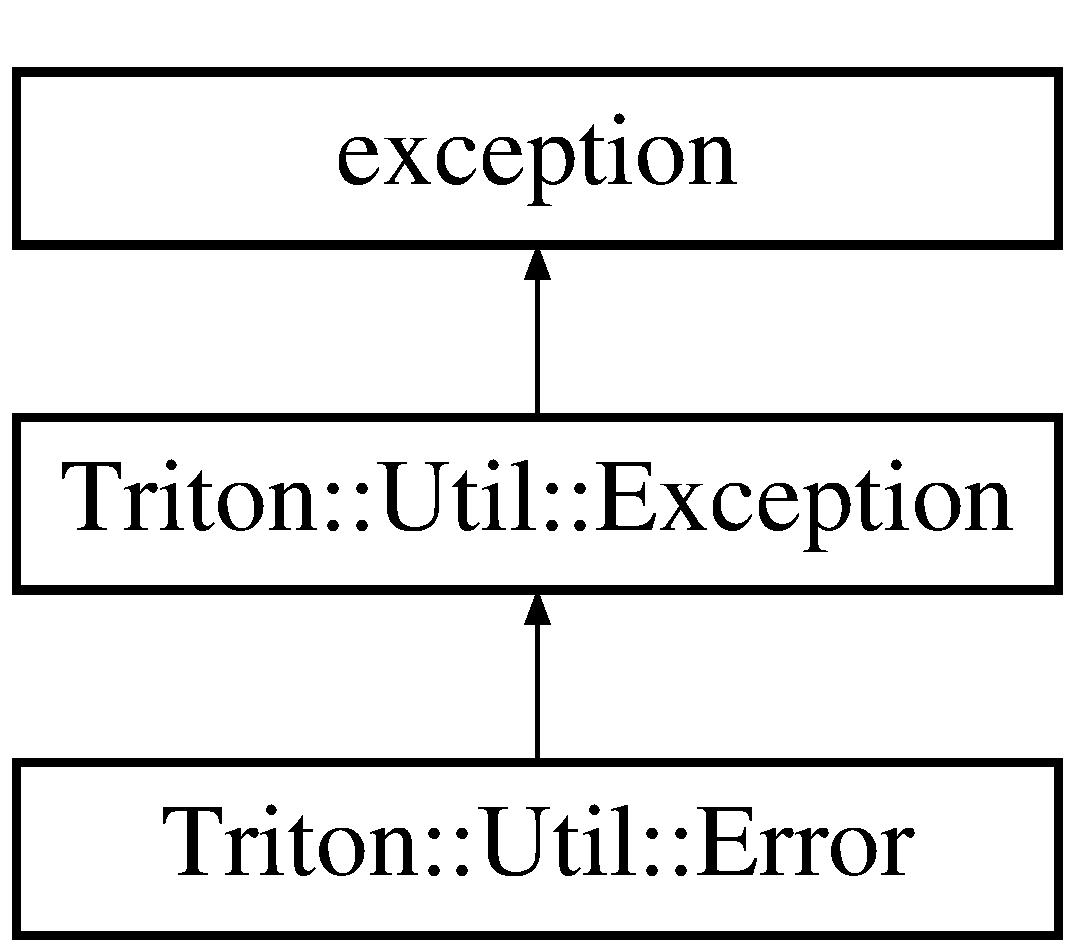
\includegraphics[height=3.000000cm]{class_triton_1_1_util_1_1_exception}
\end{center}
\end{figure}
\subsection*{Public Member Functions}
\begin{DoxyCompactItemize}
\item 
\hyperlink{class_triton_1_1_util_1_1_exception_a04987c7d05ff78f037f80b4273260ef4}{Exception} (\hyperlink{namespace_triton_1_1_util_a7e55ae91d6ccf98a52870cf7b7648eb7}{Exception\+String} msg)
\item 
virtual \hyperlink{namespace_triton_1_1_util_a7e55ae91d6ccf98a52870cf7b7648eb7}{Exception\+String} \hyperlink{class_triton_1_1_util_1_1_exception_a0465e58a2b774c528f6080f4c39ee162}{what} ()
\begin{DoxyCompactList}\small\item\em Returns the \hyperlink{namespace_triton_1_1_util_a7e55ae91d6ccf98a52870cf7b7648eb7}{Exception\+String} of this exception based on msg. \end{DoxyCompactList}\end{DoxyCompactItemize}
\subsection*{Protected Attributes}
\begin{DoxyCompactItemize}
\item 
\hyperlink{namespace_triton_1_1_util_a7e55ae91d6ccf98a52870cf7b7648eb7}{Exception\+String} \hyperlink{class_triton_1_1_util_1_1_exception_a13fcfcef497ec0336517dba8444a5687}{m\+\_\+\+Msg}
\begin{DoxyCompactList}\small\item\em The \hyperlink{namespace_triton_1_1_util_a7e55ae91d6ccf98a52870cf7b7648eb7}{Exception\+String} Message this \hyperlink{class_triton_1_1_util_1_1_exception}{Exception} gives. \end{DoxyCompactList}\end{DoxyCompactItemize}


\subsection{Detailed Description}
The basic \hyperlink{class_triton_1_1_util_1_1_exception}{Exception}. 

Definition at line 36 of file Exception.\+hpp.



\subsection{Constructor \& Destructor Documentation}
\hypertarget{class_triton_1_1_util_1_1_exception_a04987c7d05ff78f037f80b4273260ef4}{}\index{Triton\+::\+Util\+::\+Exception@{Triton\+::\+Util\+::\+Exception}!Exception@{Exception}}
\index{Exception@{Exception}!Triton\+::\+Util\+::\+Exception@{Triton\+::\+Util\+::\+Exception}}
\subsubsection[{Exception}]{\setlength{\rightskip}{0pt plus 5cm}Triton\+::\+Util\+::\+Exception\+::\+Exception (
\begin{DoxyParamCaption}
\item[{{\bf Exception\+String}}]{msg}
\end{DoxyParamCaption}
)\hspace{0.3cm}{\ttfamily [inline]}}\label{class_triton_1_1_util_1_1_exception_a04987c7d05ff78f037f80b4273260ef4}
The constructor for \hyperlink{class_triton_1_1_util_1_1_exception}{Exception}


\begin{DoxyParams}{Parameters}
{\em msg} & The message to be stored \\
\hline
\end{DoxyParams}


Definition at line 45 of file Exception.\+hpp.



\subsection{Member Function Documentation}
\hypertarget{class_triton_1_1_util_1_1_exception_a0465e58a2b774c528f6080f4c39ee162}{}\index{Triton\+::\+Util\+::\+Exception@{Triton\+::\+Util\+::\+Exception}!what@{what}}
\index{what@{what}!Triton\+::\+Util\+::\+Exception@{Triton\+::\+Util\+::\+Exception}}
\subsubsection[{what}]{\setlength{\rightskip}{0pt plus 5cm}virtual {\bf Exception\+String} Triton\+::\+Util\+::\+Exception\+::what (
\begin{DoxyParamCaption}
{}
\end{DoxyParamCaption}
)\hspace{0.3cm}{\ttfamily [inline]}, {\ttfamily [virtual]}}\label{class_triton_1_1_util_1_1_exception_a0465e58a2b774c528f6080f4c39ee162}


Returns the \hyperlink{namespace_triton_1_1_util_a7e55ae91d6ccf98a52870cf7b7648eb7}{Exception\+String} of this exception based on msg. 



Definition at line 47 of file Exception.\+hpp.



\subsection{Member Data Documentation}
\hypertarget{class_triton_1_1_util_1_1_exception_a13fcfcef497ec0336517dba8444a5687}{}\index{Triton\+::\+Util\+::\+Exception@{Triton\+::\+Util\+::\+Exception}!m\+\_\+\+Msg@{m\+\_\+\+Msg}}
\index{m\+\_\+\+Msg@{m\+\_\+\+Msg}!Triton\+::\+Util\+::\+Exception@{Triton\+::\+Util\+::\+Exception}}
\subsubsection[{m\+\_\+\+Msg}]{\setlength{\rightskip}{0pt plus 5cm}{\bf Exception\+String} Triton\+::\+Util\+::\+Exception\+::m\+\_\+\+Msg\hspace{0.3cm}{\ttfamily [protected]}}\label{class_triton_1_1_util_1_1_exception_a13fcfcef497ec0336517dba8444a5687}


The \hyperlink{namespace_triton_1_1_util_a7e55ae91d6ccf98a52870cf7b7648eb7}{Exception\+String} Message this \hyperlink{class_triton_1_1_util_1_1_exception}{Exception} gives. 



Definition at line 39 of file Exception.\+hpp.



The documentation for this class was generated from the following file\+:\begin{DoxyCompactItemize}
\item 
util/\+Exception/\hyperlink{_exception_8hpp}{Exception.\+hpp}\end{DoxyCompactItemize}

\hypertarget{class_triton_1_1_util_1_1_exception_basic_string}{}\section{Triton\+:\+:Util\+:\+:Exception\+Basic\+String$<$ char\+T $>$ Class Template Reference}
\label{class_triton_1_1_util_1_1_exception_basic_string}\index{Triton\+::\+Util\+::\+Exception\+Basic\+String$<$ char\+T $>$@{Triton\+::\+Util\+::\+Exception\+Basic\+String$<$ char\+T $>$}}


{\ttfamily \#include $<$Exception.\+hpp$>$}

\subsection*{Public Member Functions}
\begin{DoxyCompactItemize}
\item 
\hyperlink{class_triton_1_1_util_1_1_exception_basic_string_aa2af15f1d1911f2269c479f14eb7c3c9}{Exception\+Basic\+String} (const char\+T $\ast$str)
\item 
void \hyperlink{class_triton_1_1_util_1_1_exception_basic_string_a0e7d5a5cdc80660e6f3e6de9b5c9828e}{Set\+String} (const char\+T $\ast$str)
\end{DoxyCompactItemize}


\subsection{Detailed Description}
\subsubsection*{template$<$class char\+T$>$class Triton\+::\+Util\+::\+Exception\+Basic\+String$<$ char\+T $>$}

An Exception-\/\+Safe Basic String

Please use only (and only use) \hyperlink{class_triton_1_1_util_1_1_exception_basic_string}{Exception\+Basic\+String} for exception handling 

Definition at line 14 of file Exception.\+hpp.



\subsection{Constructor \& Destructor Documentation}
\hypertarget{class_triton_1_1_util_1_1_exception_basic_string_aa2af15f1d1911f2269c479f14eb7c3c9}{}\index{Triton\+::\+Util\+::\+Exception\+Basic\+String@{Triton\+::\+Util\+::\+Exception\+Basic\+String}!Exception\+Basic\+String@{Exception\+Basic\+String}}
\index{Exception\+Basic\+String@{Exception\+Basic\+String}!Triton\+::\+Util\+::\+Exception\+Basic\+String@{Triton\+::\+Util\+::\+Exception\+Basic\+String}}
\subsubsection[{Exception\+Basic\+String}]{\setlength{\rightskip}{0pt plus 5cm}template$<$class char\+T$>$ {\bf Triton\+::\+Util\+::\+Exception\+Basic\+String}$<$ char\+T $>$\+::{\bf Exception\+Basic\+String} (
\begin{DoxyParamCaption}
\item[{const char\+T $\ast$}]{str}
\end{DoxyParamCaption}
)}\label{class_triton_1_1_util_1_1_exception_basic_string_aa2af15f1d1911f2269c479f14eb7c3c9}


\subsection{Member Function Documentation}
\hypertarget{class_triton_1_1_util_1_1_exception_basic_string_a0e7d5a5cdc80660e6f3e6de9b5c9828e}{}\index{Triton\+::\+Util\+::\+Exception\+Basic\+String@{Triton\+::\+Util\+::\+Exception\+Basic\+String}!Set\+String@{Set\+String}}
\index{Set\+String@{Set\+String}!Triton\+::\+Util\+::\+Exception\+Basic\+String@{Triton\+::\+Util\+::\+Exception\+Basic\+String}}
\subsubsection[{Set\+String}]{\setlength{\rightskip}{0pt plus 5cm}template$<$class char\+T$>$ void {\bf Triton\+::\+Util\+::\+Exception\+Basic\+String}$<$ char\+T $>$\+::Set\+String (
\begin{DoxyParamCaption}
\item[{const char\+T $\ast$}]{str}
\end{DoxyParamCaption}
)\hspace{0.3cm}{\ttfamily [inline]}}\label{class_triton_1_1_util_1_1_exception_basic_string_a0e7d5a5cdc80660e6f3e6de9b5c9828e}


Definition at line 21 of file Exception.\+hpp.



The documentation for this class was generated from the following file\+:\begin{DoxyCompactItemize}
\item 
util/\+Exception/\hyperlink{_exception_8hpp}{Exception.\+hpp}\end{DoxyCompactItemize}

\hypertarget{class_tri_1_1_graphic_1_1_graphical_exception}{}\section{Tri\+:\+:Graphic\+:\+:Graphical\+Exception Class Reference}
\label{class_tri_1_1_graphic_1_1_graphical_exception}\index{Tri\+::\+Graphic\+::\+Graphical\+Exception@{Tri\+::\+Graphic\+::\+Graphical\+Exception}}


{\ttfamily \#include $<$util.\+h$>$}

Inheritance diagram for Tri\+:\+:Graphic\+:\+:Graphical\+Exception\+:\begin{figure}[H]
\begin{center}
\leavevmode
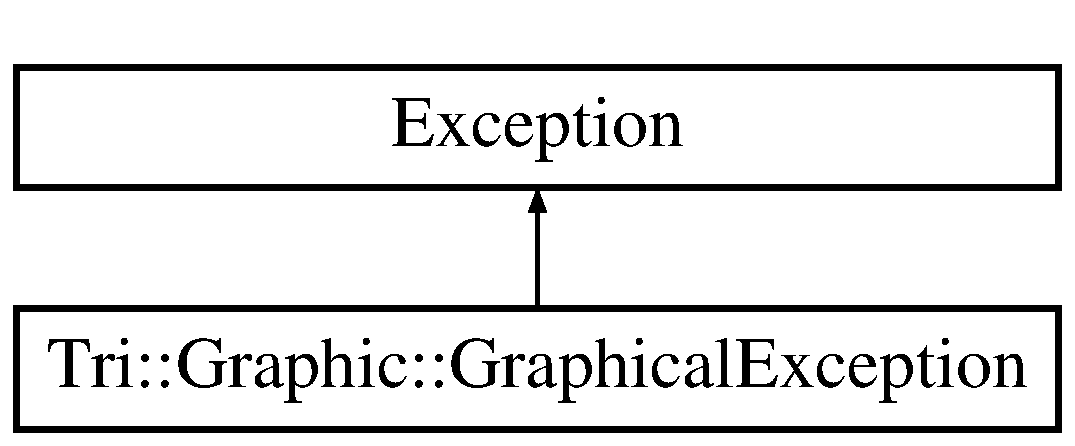
\includegraphics[height=2.000000cm]{class_tri_1_1_graphic_1_1_graphical_exception}
\end{center}
\end{figure}
\subsection*{Public Member Functions}
\begin{DoxyCompactItemize}
\item 
\hyperlink{class_tri_1_1_graphic_1_1_graphical_exception_a588edbbc3986a081be5d776037906165}{Graphical\+Exception} (L\+U\+S\+::\+String msg)
\end{DoxyCompactItemize}


\subsection{Detailed Description}


Definition at line 14 of file util.\+h.



\subsection{Constructor \& Destructor Documentation}
\hypertarget{class_tri_1_1_graphic_1_1_graphical_exception_a588edbbc3986a081be5d776037906165}{}\index{Tri\+::\+Graphic\+::\+Graphical\+Exception@{Tri\+::\+Graphic\+::\+Graphical\+Exception}!Graphical\+Exception@{Graphical\+Exception}}
\index{Graphical\+Exception@{Graphical\+Exception}!Tri\+::\+Graphic\+::\+Graphical\+Exception@{Tri\+::\+Graphic\+::\+Graphical\+Exception}}
\subsubsection[{Graphical\+Exception}]{\setlength{\rightskip}{0pt plus 5cm}Tri\+::\+Graphic\+::\+Graphical\+Exception\+::\+Graphical\+Exception (
\begin{DoxyParamCaption}
\item[{L\+U\+S\+::\+String}]{msg}
\end{DoxyParamCaption}
)\hspace{0.3cm}{\ttfamily [inline]}}\label{class_tri_1_1_graphic_1_1_graphical_exception_a588edbbc3986a081be5d776037906165}


Definition at line 17 of file util.\+h.



The documentation for this class was generated from the following file\+:\begin{DoxyCompactItemize}
\item 
graphic/\hyperlink{graphic_2util_8h}{util.\+h}\end{DoxyCompactItemize}

\hypertarget{class_tri_1_1_graphic_1_1_graphic_manager}{}\section{Tri\+:\+:Graphic\+:\+:Graphic\+Manager Class Reference}
\label{class_tri_1_1_graphic_1_1_graphic_manager}\index{Tri\+::\+Graphic\+::\+Graphic\+Manager@{Tri\+::\+Graphic\+::\+Graphic\+Manager}}


{\ttfamily \#include $<$util.\+h$>$}

\subsection*{Public Member Functions}
\begin{DoxyCompactItemize}
\item 
\hyperlink{class_tri_1_1_graphic_1_1_graphic_manager_a1c859cd3579ac7f174f41155e9e850e4}{Open\+G\+L\+Manager} ()
\item 
\hyperlink{class_tri_1_1_graphic_1_1_graphic_manager_a472fe570c5cc75942330bf3b4a137d32}{$\sim$\+Open\+G\+L\+Manager} ()
\item 
Render\+::\+Draw\+Object $\ast$ \hyperlink{class_tri_1_1_graphic_1_1_graphic_manager_aab2ac5b4847dcdf9083ab3cc88cbd285}{Add\+Drawable} (Render\+::\+Draw\+Object $\ast$p\+Draw)
\begin{DoxyCompactList}\small\item\em Simple addition of drawable objects. \end{DoxyCompactList}\item 
glsettings\+\_\+t $\ast$ \hyperlink{class_tri_1_1_graphic_1_1_graphic_manager_a3d5a8e96349899110189d6fdb6f07aea}{Get\+Settings} ()
\begin{DoxyCompactList}\small\item\em Retrieves the current (mutable) settings. \end{DoxyCompactList}\item 
\hyperlink{namespace_tri_1_1_graphic_a7b3538cdaff9bf96489c56a4f48a5f9a}{Mat4} \hyperlink{class_tri_1_1_graphic_1_1_graphic_manager_a00d8bb1aec0fe078ebcc66a338eedd3b}{Get\+Projection\+Matrix} ()
\item 
\hyperlink{namespace_tri_1_1_graphic_a7b3538cdaff9bf96489c56a4f48a5f9a}{Mat4} \hyperlink{class_tri_1_1_graphic_1_1_graphic_manager_a127658447d27febc589df6207773f07b}{Get\+M\+V\+P\+For} (Render\+::\+I\+Draw draw)
\item 
unsigned int \hyperlink{class_tri_1_1_graphic_1_1_graphic_manager_ad877d9503a37f69f6406474e08772676}{Get\+Tick\+Update} ()
\item 
void \hyperlink{class_tri_1_1_graphic_1_1_graphic_manager_a63a7dee2163f0bbfd5eb1acd35c1d17f}{Render} ()
\item 
bool \hyperlink{class_tri_1_1_graphic_1_1_graphic_manager_a22a887c39e00775be78981ca95cd9ea6}{Is3\+D\+Enabled} ()
\end{DoxyCompactItemize}


\subsection{Detailed Description}


Definition at line 20 of file util.\+h.



\subsection{Constructor \& Destructor Documentation}
\hypertarget{class_tri_1_1_graphic_1_1_graphic_manager_a472fe570c5cc75942330bf3b4a137d32}{}\index{Tri\+::\+Graphic\+::\+Graphic\+Manager@{Tri\+::\+Graphic\+::\+Graphic\+Manager}!````~Open\+G\+L\+Manager@{$\sim$\+Open\+G\+L\+Manager}}
\index{````~Open\+G\+L\+Manager@{$\sim$\+Open\+G\+L\+Manager}!Tri\+::\+Graphic\+::\+Graphic\+Manager@{Tri\+::\+Graphic\+::\+Graphic\+Manager}}
\subsubsection[{$\sim$\+Open\+G\+L\+Manager}]{\setlength{\rightskip}{0pt plus 5cm}Tri\+::\+Graphic\+::\+Graphic\+Manager\+::$\sim$\+Open\+G\+L\+Manager (
\begin{DoxyParamCaption}
{}
\end{DoxyParamCaption}
)}\label{class_tri_1_1_graphic_1_1_graphic_manager_a472fe570c5cc75942330bf3b4a137d32}


\subsection{Member Function Documentation}
\hypertarget{class_tri_1_1_graphic_1_1_graphic_manager_aab2ac5b4847dcdf9083ab3cc88cbd285}{}\index{Tri\+::\+Graphic\+::\+Graphic\+Manager@{Tri\+::\+Graphic\+::\+Graphic\+Manager}!Add\+Drawable@{Add\+Drawable}}
\index{Add\+Drawable@{Add\+Drawable}!Tri\+::\+Graphic\+::\+Graphic\+Manager@{Tri\+::\+Graphic\+::\+Graphic\+Manager}}
\subsubsection[{Add\+Drawable}]{\setlength{\rightskip}{0pt plus 5cm}Render\+::\+Draw\+Object$\ast$ Tri\+::\+Graphic\+::\+Graphic\+Manager\+::\+Add\+Drawable (
\begin{DoxyParamCaption}
\item[{Render\+::\+Draw\+Object $\ast$}]{p\+Draw}
\end{DoxyParamCaption}
)}\label{class_tri_1_1_graphic_1_1_graphic_manager_aab2ac5b4847dcdf9083ab3cc88cbd285}


Simple addition of drawable objects. 


\begin{DoxyParams}{Parameters}
{\em p\+Draw} & A pointer to a drawable object defined by L\+E\+A\+K\+\_\+\+U\+S\+E\+\_\+2\+D, 2\+D only if stated, 3\+D otherwsie \\
\hline
\end{DoxyParams}
\hypertarget{class_tri_1_1_graphic_1_1_graphic_manager_a127658447d27febc589df6207773f07b}{}\index{Tri\+::\+Graphic\+::\+Graphic\+Manager@{Tri\+::\+Graphic\+::\+Graphic\+Manager}!Get\+M\+V\+P\+For@{Get\+M\+V\+P\+For}}
\index{Get\+M\+V\+P\+For@{Get\+M\+V\+P\+For}!Tri\+::\+Graphic\+::\+Graphic\+Manager@{Tri\+::\+Graphic\+::\+Graphic\+Manager}}
\subsubsection[{Get\+M\+V\+P\+For}]{\setlength{\rightskip}{0pt plus 5cm}{\bf Mat4} Tri\+::\+Graphic\+::\+Graphic\+Manager\+::\+Get\+M\+V\+P\+For (
\begin{DoxyParamCaption}
\item[{Render\+::\+I\+Draw}]{draw}
\end{DoxyParamCaption}
)}\label{class_tri_1_1_graphic_1_1_graphic_manager_a127658447d27febc589df6207773f07b}
\hypertarget{class_tri_1_1_graphic_1_1_graphic_manager_a00d8bb1aec0fe078ebcc66a338eedd3b}{}\index{Tri\+::\+Graphic\+::\+Graphic\+Manager@{Tri\+::\+Graphic\+::\+Graphic\+Manager}!Get\+Projection\+Matrix@{Get\+Projection\+Matrix}}
\index{Get\+Projection\+Matrix@{Get\+Projection\+Matrix}!Tri\+::\+Graphic\+::\+Graphic\+Manager@{Tri\+::\+Graphic\+::\+Graphic\+Manager}}
\subsubsection[{Get\+Projection\+Matrix}]{\setlength{\rightskip}{0pt plus 5cm}{\bf Mat4} Tri\+::\+Graphic\+::\+Graphic\+Manager\+::\+Get\+Projection\+Matrix (
\begin{DoxyParamCaption}
{}
\end{DoxyParamCaption}
)}\label{class_tri_1_1_graphic_1_1_graphic_manager_a00d8bb1aec0fe078ebcc66a338eedd3b}
\hypertarget{class_tri_1_1_graphic_1_1_graphic_manager_a3d5a8e96349899110189d6fdb6f07aea}{}\index{Tri\+::\+Graphic\+::\+Graphic\+Manager@{Tri\+::\+Graphic\+::\+Graphic\+Manager}!Get\+Settings@{Get\+Settings}}
\index{Get\+Settings@{Get\+Settings}!Tri\+::\+Graphic\+::\+Graphic\+Manager@{Tri\+::\+Graphic\+::\+Graphic\+Manager}}
\subsubsection[{Get\+Settings}]{\setlength{\rightskip}{0pt plus 5cm}glsettings\+\_\+t$\ast$ Tri\+::\+Graphic\+::\+Graphic\+Manager\+::\+Get\+Settings (
\begin{DoxyParamCaption}
{}
\end{DoxyParamCaption}
)}\label{class_tri_1_1_graphic_1_1_graphic_manager_a3d5a8e96349899110189d6fdb6f07aea}


Retrieves the current (mutable) settings. 

\hypertarget{class_tri_1_1_graphic_1_1_graphic_manager_ad877d9503a37f69f6406474e08772676}{}\index{Tri\+::\+Graphic\+::\+Graphic\+Manager@{Tri\+::\+Graphic\+::\+Graphic\+Manager}!Get\+Tick\+Update@{Get\+Tick\+Update}}
\index{Get\+Tick\+Update@{Get\+Tick\+Update}!Tri\+::\+Graphic\+::\+Graphic\+Manager@{Tri\+::\+Graphic\+::\+Graphic\+Manager}}
\subsubsection[{Get\+Tick\+Update}]{\setlength{\rightskip}{0pt plus 5cm}unsigned int Tri\+::\+Graphic\+::\+Graphic\+Manager\+::\+Get\+Tick\+Update (
\begin{DoxyParamCaption}
{}
\end{DoxyParamCaption}
)}\label{class_tri_1_1_graphic_1_1_graphic_manager_ad877d9503a37f69f6406474e08772676}
\hypertarget{class_tri_1_1_graphic_1_1_graphic_manager_a22a887c39e00775be78981ca95cd9ea6}{}\index{Tri\+::\+Graphic\+::\+Graphic\+Manager@{Tri\+::\+Graphic\+::\+Graphic\+Manager}!Is3\+D\+Enabled@{Is3\+D\+Enabled}}
\index{Is3\+D\+Enabled@{Is3\+D\+Enabled}!Tri\+::\+Graphic\+::\+Graphic\+Manager@{Tri\+::\+Graphic\+::\+Graphic\+Manager}}
\subsubsection[{Is3\+D\+Enabled}]{\setlength{\rightskip}{0pt plus 5cm}bool Tri\+::\+Graphic\+::\+Graphic\+Manager\+::\+Is3\+D\+Enabled (
\begin{DoxyParamCaption}
{}
\end{DoxyParamCaption}
)\hspace{0.3cm}{\ttfamily [inline]}}\label{class_tri_1_1_graphic_1_1_graphic_manager_a22a887c39e00775be78981ca95cd9ea6}


Definition at line 56 of file util.\+h.

\hypertarget{class_tri_1_1_graphic_1_1_graphic_manager_a1c859cd3579ac7f174f41155e9e850e4}{}\index{Tri\+::\+Graphic\+::\+Graphic\+Manager@{Tri\+::\+Graphic\+::\+Graphic\+Manager}!Open\+G\+L\+Manager@{Open\+G\+L\+Manager}}
\index{Open\+G\+L\+Manager@{Open\+G\+L\+Manager}!Tri\+::\+Graphic\+::\+Graphic\+Manager@{Tri\+::\+Graphic\+::\+Graphic\+Manager}}
\subsubsection[{Open\+G\+L\+Manager}]{\setlength{\rightskip}{0pt plus 5cm}Tri\+::\+Graphic\+::\+Graphic\+Manager\+::\+Open\+G\+L\+Manager (
\begin{DoxyParamCaption}
{}
\end{DoxyParamCaption}
)}\label{class_tri_1_1_graphic_1_1_graphic_manager_a1c859cd3579ac7f174f41155e9e850e4}
\hypertarget{class_tri_1_1_graphic_1_1_graphic_manager_a63a7dee2163f0bbfd5eb1acd35c1d17f}{}\index{Tri\+::\+Graphic\+::\+Graphic\+Manager@{Tri\+::\+Graphic\+::\+Graphic\+Manager}!Render@{Render}}
\index{Render@{Render}!Tri\+::\+Graphic\+::\+Graphic\+Manager@{Tri\+::\+Graphic\+::\+Graphic\+Manager}}
\subsubsection[{Render}]{\setlength{\rightskip}{0pt plus 5cm}void Tri\+::\+Graphic\+::\+Graphic\+Manager\+::\+Render (
\begin{DoxyParamCaption}
{}
\end{DoxyParamCaption}
)}\label{class_tri_1_1_graphic_1_1_graphic_manager_a63a7dee2163f0bbfd5eb1acd35c1d17f}


The documentation for this class was generated from the following file\+:\begin{DoxyCompactItemize}
\item 
graphic/\hyperlink{graphic_2util_8h}{util.\+h}\end{DoxyCompactItemize}

\hypertarget{class_tri_1_1_graphic_1_1_i_draw}{}\section{Tri\+:\+:Graphic\+:\+:I\+Draw Class Reference}
\label{class_tri_1_1_graphic_1_1_i_draw}\index{Tri\+::\+Graphic\+::\+I\+Draw@{Tri\+::\+Graphic\+::\+I\+Draw}}


{\ttfamily \#include $<$render.\+h$>$}

Inheritance diagram for Tri\+:\+:Graphic\+:\+:I\+Draw\+:\begin{figure}[H]
\begin{center}
\leavevmode
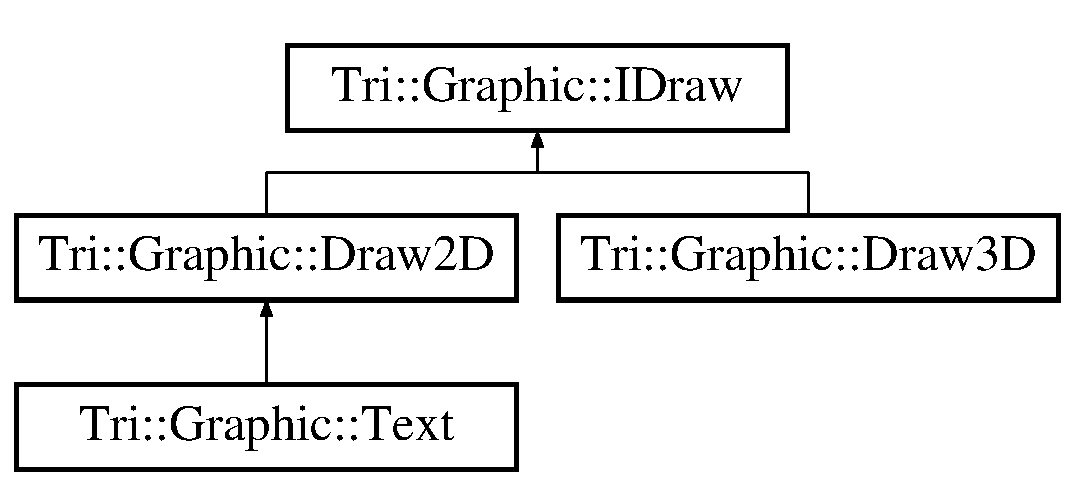
\includegraphics[height=3.000000cm]{class_tri_1_1_graphic_1_1_i_draw}
\end{center}
\end{figure}
\subsection*{Public Member Functions}
\begin{DoxyCompactItemize}
\item 
virtual void \hyperlink{class_tri_1_1_graphic_1_1_i_draw_ae1b4dd358a248d39a9e9e586e95c7805}{Update} (int tick)=0
\begin{DoxyCompactList}\small\item\em The logical update function for \hyperlink{class_tri_1_1_graphic_1_1_i_draw}{I\+Draw}. \end{DoxyCompactList}\item 
virtual void \hyperlink{class_tri_1_1_graphic_1_1_i_draw_a27e0987b4969055048a12691f00de4a5}{Render} ()=0
\begin{DoxyCompactList}\small\item\em The graphical function for \hyperlink{class_tri_1_1_graphic_1_1_i_draw}{I\+Draw}. \end{DoxyCompactList}\item 
Shader\+::\+Shader\+Program \hyperlink{class_tri_1_1_graphic_1_1_i_draw_ad5b23c2e7f64b7420632fc110281e670}{Get\+Shader} ()
\item 
virtual \hyperlink{namespace_tri_1_1_graphic_a7b3538cdaff9bf96489c56a4f48a5f9a}{Mat4} \hyperlink{class_tri_1_1_graphic_1_1_i_draw_ae6c6b2e08c6d6e2d4f8a07b24de0018c}{Get\+Model\+Matrix} ()=0
\end{DoxyCompactItemize}
\subsection*{Public Attributes}
\begin{DoxyCompactItemize}
\item 
bool \hyperlink{class_tri_1_1_graphic_1_1_i_draw_af3a5753923c1b956b56194f8d12a3405}{m\+Keep\+Up} = false
\begin{DoxyCompactList}\small\item\em Boolean to determine whether to keep the object up after closing the \hyperlink{namespace_tri_1_1_graphic}{Graphic} Engine. \end{DoxyCompactList}\end{DoxyCompactItemize}
\subsection*{Protected Attributes}
\begin{DoxyCompactItemize}
\item 
unsigned long \hyperlink{class_tri_1_1_graphic_1_1_i_draw_a8e15d0b6ba0dc7439d4a2cd13da1cda0}{m\+Id}
\item 
Shader\+::\+Shader\+Program \hyperlink{class_tri_1_1_graphic_1_1_i_draw_a37fb2171ca69c8f803c0266814c7296b}{m\+Shader\+Program}
\end{DoxyCompactItemize}


\subsection{Detailed Description}


Definition at line 44 of file render.\+h.



\subsection{Member Function Documentation}
\hypertarget{class_tri_1_1_graphic_1_1_i_draw_ae6c6b2e08c6d6e2d4f8a07b24de0018c}{}\index{Tri\+::\+Graphic\+::\+I\+Draw@{Tri\+::\+Graphic\+::\+I\+Draw}!Get\+Model\+Matrix@{Get\+Model\+Matrix}}
\index{Get\+Model\+Matrix@{Get\+Model\+Matrix}!Tri\+::\+Graphic\+::\+I\+Draw@{Tri\+::\+Graphic\+::\+I\+Draw}}
\subsubsection[{Get\+Model\+Matrix}]{\setlength{\rightskip}{0pt plus 5cm}virtual {\bf Mat4} Tri\+::\+Graphic\+::\+I\+Draw\+::\+Get\+Model\+Matrix (
\begin{DoxyParamCaption}
{}
\end{DoxyParamCaption}
)\hspace{0.3cm}{\ttfamily [pure virtual]}}\label{class_tri_1_1_graphic_1_1_i_draw_ae6c6b2e08c6d6e2d4f8a07b24de0018c}


Implemented in \hyperlink{class_tri_1_1_graphic_1_1_draw3_d_a32ab7b7f0f956c0058a4a24a20ff4efc}{Tri\+::\+Graphic\+::\+Draw3\+D}, and \hyperlink{class_tri_1_1_graphic_1_1_draw2_d_ab9fda1624fd99c6ab7d05e8a9aa2b4bd}{Tri\+::\+Graphic\+::\+Draw2\+D}.

\hypertarget{class_tri_1_1_graphic_1_1_i_draw_ad5b23c2e7f64b7420632fc110281e670}{}\index{Tri\+::\+Graphic\+::\+I\+Draw@{Tri\+::\+Graphic\+::\+I\+Draw}!Get\+Shader@{Get\+Shader}}
\index{Get\+Shader@{Get\+Shader}!Tri\+::\+Graphic\+::\+I\+Draw@{Tri\+::\+Graphic\+::\+I\+Draw}}
\subsubsection[{Get\+Shader}]{\setlength{\rightskip}{0pt plus 5cm}Shader\+::\+Shader\+Program Tri\+::\+Graphic\+::\+I\+Draw\+::\+Get\+Shader (
\begin{DoxyParamCaption}
{}
\end{DoxyParamCaption}
)}\label{class_tri_1_1_graphic_1_1_i_draw_ad5b23c2e7f64b7420632fc110281e670}
\hypertarget{class_tri_1_1_graphic_1_1_i_draw_a27e0987b4969055048a12691f00de4a5}{}\index{Tri\+::\+Graphic\+::\+I\+Draw@{Tri\+::\+Graphic\+::\+I\+Draw}!Render@{Render}}
\index{Render@{Render}!Tri\+::\+Graphic\+::\+I\+Draw@{Tri\+::\+Graphic\+::\+I\+Draw}}
\subsubsection[{Render}]{\setlength{\rightskip}{0pt plus 5cm}virtual void Tri\+::\+Graphic\+::\+I\+Draw\+::\+Render (
\begin{DoxyParamCaption}
{}
\end{DoxyParamCaption}
)\hspace{0.3cm}{\ttfamily [pure virtual]}}\label{class_tri_1_1_graphic_1_1_i_draw_a27e0987b4969055048a12691f00de4a5}


The graphical function for \hyperlink{class_tri_1_1_graphic_1_1_i_draw}{I\+Draw}. 

Use for Graphical Manipulations \hypertarget{class_tri_1_1_graphic_1_1_i_draw_ae1b4dd358a248d39a9e9e586e95c7805}{}\index{Tri\+::\+Graphic\+::\+I\+Draw@{Tri\+::\+Graphic\+::\+I\+Draw}!Update@{Update}}
\index{Update@{Update}!Tri\+::\+Graphic\+::\+I\+Draw@{Tri\+::\+Graphic\+::\+I\+Draw}}
\subsubsection[{Update}]{\setlength{\rightskip}{0pt plus 5cm}virtual void Tri\+::\+Graphic\+::\+I\+Draw\+::\+Update (
\begin{DoxyParamCaption}
\item[{int}]{tick}
\end{DoxyParamCaption}
)\hspace{0.3cm}{\ttfamily [pure virtual]}}\label{class_tri_1_1_graphic_1_1_i_draw_ae1b4dd358a248d39a9e9e586e95c7805}


The logical update function for \hyperlink{class_tri_1_1_graphic_1_1_i_draw}{I\+Draw}. 

Use for positional changes 

\subsection{Member Data Documentation}
\hypertarget{class_tri_1_1_graphic_1_1_i_draw_a8e15d0b6ba0dc7439d4a2cd13da1cda0}{}\index{Tri\+::\+Graphic\+::\+I\+Draw@{Tri\+::\+Graphic\+::\+I\+Draw}!m\+Id@{m\+Id}}
\index{m\+Id@{m\+Id}!Tri\+::\+Graphic\+::\+I\+Draw@{Tri\+::\+Graphic\+::\+I\+Draw}}
\subsubsection[{m\+Id}]{\setlength{\rightskip}{0pt plus 5cm}unsigned long Tri\+::\+Graphic\+::\+I\+Draw\+::m\+Id\hspace{0.3cm}{\ttfamily [protected]}}\label{class_tri_1_1_graphic_1_1_i_draw_a8e15d0b6ba0dc7439d4a2cd13da1cda0}


Definition at line 47 of file render.\+h.

\hypertarget{class_tri_1_1_graphic_1_1_i_draw_af3a5753923c1b956b56194f8d12a3405}{}\index{Tri\+::\+Graphic\+::\+I\+Draw@{Tri\+::\+Graphic\+::\+I\+Draw}!m\+Keep\+Up@{m\+Keep\+Up}}
\index{m\+Keep\+Up@{m\+Keep\+Up}!Tri\+::\+Graphic\+::\+I\+Draw@{Tri\+::\+Graphic\+::\+I\+Draw}}
\subsubsection[{m\+Keep\+Up}]{\setlength{\rightskip}{0pt plus 5cm}bool Tri\+::\+Graphic\+::\+I\+Draw\+::m\+Keep\+Up = false}\label{class_tri_1_1_graphic_1_1_i_draw_af3a5753923c1b956b56194f8d12a3405}


Boolean to determine whether to keep the object up after closing the \hyperlink{namespace_tri_1_1_graphic}{Graphic} Engine. 



Definition at line 50 of file render.\+h.

\hypertarget{class_tri_1_1_graphic_1_1_i_draw_a37fb2171ca69c8f803c0266814c7296b}{}\index{Tri\+::\+Graphic\+::\+I\+Draw@{Tri\+::\+Graphic\+::\+I\+Draw}!m\+Shader\+Program@{m\+Shader\+Program}}
\index{m\+Shader\+Program@{m\+Shader\+Program}!Tri\+::\+Graphic\+::\+I\+Draw@{Tri\+::\+Graphic\+::\+I\+Draw}}
\subsubsection[{m\+Shader\+Program}]{\setlength{\rightskip}{0pt plus 5cm}Shader\+::\+Shader\+Program Tri\+::\+Graphic\+::\+I\+Draw\+::m\+Shader\+Program\hspace{0.3cm}{\ttfamily [protected]}}\label{class_tri_1_1_graphic_1_1_i_draw_a37fb2171ca69c8f803c0266814c7296b}


Definition at line 48 of file render.\+h.



The documentation for this class was generated from the following file\+:\begin{DoxyCompactItemize}
\item 
graphic/\hyperlink{render_8h}{render.\+h}\end{DoxyCompactItemize}

\hypertarget{class_tri_1_1_graphic_1_1_image}{}\section{Tri\+:\+:Graphic\+:\+:Image Class Reference}
\label{class_tri_1_1_graphic_1_1_image}\index{Tri\+::\+Graphic\+::\+Image@{Tri\+::\+Graphic\+::\+Image}}


{\ttfamily \#include $<$resource.\+h$>$}

\subsection*{Public Member Functions}
\begin{DoxyCompactItemize}
\item 
\hyperlink{class_tri_1_1_graphic_1_1_image_a6b643da93b3fb2c4dd49615b72a3a0d5}{Image} (unsigned int width, unsigned int height, const L\+U\+S\+::ubyte $\ast$data)
\item 
\hyperlink{class_tri_1_1_graphic_1_1_image_af1a11b13c3544391e470b66103c8f355}{Image} (unsigned int texure\+Id)
\item 
unsigned int \hyperlink{class_tri_1_1_graphic_1_1_image_a4cf866cbf689b64d901576b70a1bf692}{Get\+Texture\+Id} ()
\item 
void \hyperlink{class_tri_1_1_graphic_1_1_image_a389344f423410008278a810945cdb5f7}{Draw} ()
\end{DoxyCompactItemize}
\subsection*{Static Public Member Functions}
\begin{DoxyCompactItemize}
\item 
static \hyperlink{class_tri_1_1_graphic_1_1_image}{Image} \hyperlink{class_tri_1_1_graphic_1_1_image_a032c706644e420edcddabfc0ee93f1ce}{Get\+Bmp} (Util\+::\+String filepath)
\item 
static \hyperlink{class_tri_1_1_graphic_1_1_image}{Image} \hyperlink{class_tri_1_1_graphic_1_1_image_a9769601595adf7084c01c999de322264}{Get\+Dds} (Util\+::\+String filepath)
\end{DoxyCompactItemize}


\subsection{Detailed Description}


Definition at line 13 of file resource.\+h.



\subsection{Constructor \& Destructor Documentation}
\hypertarget{class_tri_1_1_graphic_1_1_image_a6b643da93b3fb2c4dd49615b72a3a0d5}{}\index{Tri\+::\+Graphic\+::\+Image@{Tri\+::\+Graphic\+::\+Image}!Image@{Image}}
\index{Image@{Image}!Tri\+::\+Graphic\+::\+Image@{Tri\+::\+Graphic\+::\+Image}}
\subsubsection[{Image}]{\setlength{\rightskip}{0pt plus 5cm}Tri\+::\+Graphic\+::\+Image\+::\+Image (
\begin{DoxyParamCaption}
\item[{unsigned int}]{width, }
\item[{unsigned int}]{height, }
\item[{const L\+U\+S\+::ubyte $\ast$}]{data}
\end{DoxyParamCaption}
)}\label{class_tri_1_1_graphic_1_1_image_a6b643da93b3fb2c4dd49615b72a3a0d5}
\hypertarget{class_tri_1_1_graphic_1_1_image_af1a11b13c3544391e470b66103c8f355}{}\index{Tri\+::\+Graphic\+::\+Image@{Tri\+::\+Graphic\+::\+Image}!Image@{Image}}
\index{Image@{Image}!Tri\+::\+Graphic\+::\+Image@{Tri\+::\+Graphic\+::\+Image}}
\subsubsection[{Image}]{\setlength{\rightskip}{0pt plus 5cm}Tri\+::\+Graphic\+::\+Image\+::\+Image (
\begin{DoxyParamCaption}
\item[{unsigned int}]{texure\+Id}
\end{DoxyParamCaption}
)}\label{class_tri_1_1_graphic_1_1_image_af1a11b13c3544391e470b66103c8f355}


\subsection{Member Function Documentation}
\hypertarget{class_tri_1_1_graphic_1_1_image_a389344f423410008278a810945cdb5f7}{}\index{Tri\+::\+Graphic\+::\+Image@{Tri\+::\+Graphic\+::\+Image}!Draw@{Draw}}
\index{Draw@{Draw}!Tri\+::\+Graphic\+::\+Image@{Tri\+::\+Graphic\+::\+Image}}
\subsubsection[{Draw}]{\setlength{\rightskip}{0pt plus 5cm}void Tri\+::\+Graphic\+::\+Image\+::\+Draw (
\begin{DoxyParamCaption}
{}
\end{DoxyParamCaption}
)}\label{class_tri_1_1_graphic_1_1_image_a389344f423410008278a810945cdb5f7}
\hypertarget{class_tri_1_1_graphic_1_1_image_a032c706644e420edcddabfc0ee93f1ce}{}\index{Tri\+::\+Graphic\+::\+Image@{Tri\+::\+Graphic\+::\+Image}!Get\+Bmp@{Get\+Bmp}}
\index{Get\+Bmp@{Get\+Bmp}!Tri\+::\+Graphic\+::\+Image@{Tri\+::\+Graphic\+::\+Image}}
\subsubsection[{Get\+Bmp}]{\setlength{\rightskip}{0pt plus 5cm}static {\bf Image} Tri\+::\+Graphic\+::\+Image\+::\+Get\+Bmp (
\begin{DoxyParamCaption}
\item[{Util\+::\+String}]{filepath}
\end{DoxyParamCaption}
)\hspace{0.3cm}{\ttfamily [static]}}\label{class_tri_1_1_graphic_1_1_image_a032c706644e420edcddabfc0ee93f1ce}
\hypertarget{class_tri_1_1_graphic_1_1_image_a9769601595adf7084c01c999de322264}{}\index{Tri\+::\+Graphic\+::\+Image@{Tri\+::\+Graphic\+::\+Image}!Get\+Dds@{Get\+Dds}}
\index{Get\+Dds@{Get\+Dds}!Tri\+::\+Graphic\+::\+Image@{Tri\+::\+Graphic\+::\+Image}}
\subsubsection[{Get\+Dds}]{\setlength{\rightskip}{0pt plus 5cm}static {\bf Image} Tri\+::\+Graphic\+::\+Image\+::\+Get\+Dds (
\begin{DoxyParamCaption}
\item[{Util\+::\+String}]{filepath}
\end{DoxyParamCaption}
)\hspace{0.3cm}{\ttfamily [static]}}\label{class_tri_1_1_graphic_1_1_image_a9769601595adf7084c01c999de322264}
\hypertarget{class_tri_1_1_graphic_1_1_image_a4cf866cbf689b64d901576b70a1bf692}{}\index{Tri\+::\+Graphic\+::\+Image@{Tri\+::\+Graphic\+::\+Image}!Get\+Texture\+Id@{Get\+Texture\+Id}}
\index{Get\+Texture\+Id@{Get\+Texture\+Id}!Tri\+::\+Graphic\+::\+Image@{Tri\+::\+Graphic\+::\+Image}}
\subsubsection[{Get\+Texture\+Id}]{\setlength{\rightskip}{0pt plus 5cm}unsigned int Tri\+::\+Graphic\+::\+Image\+::\+Get\+Texture\+Id (
\begin{DoxyParamCaption}
{}
\end{DoxyParamCaption}
)}\label{class_tri_1_1_graphic_1_1_image_a4cf866cbf689b64d901576b70a1bf692}


The documentation for this class was generated from the following file\+:\begin{DoxyCompactItemize}
\item 
graphic/\hyperlink{resource_8h}{resource.\+h}\end{DoxyCompactItemize}

\hypertarget{struct_tri_1_1_input_1_1_input_interface}{}\section{Tri\+:\+:Input\+:\+:Input\+Interface Struct Reference}
\label{struct_tri_1_1_input_1_1_input_interface}\index{Tri\+::\+Input\+::\+Input\+Interface@{Tri\+::\+Input\+::\+Input\+Interface}}


{\ttfamily \#include $<$util.\+h$>$}

\subsection*{Public Member Functions}
\begin{DoxyCompactItemize}
\item 
virtual \hyperlink{struct_tri_1_1_input_1_1_input_interface_a7e7ef1cdb89376ce9e85215474377fa2}{Input\+Interface} ()
\item 
virtual \hyperlink{struct_tri_1_1_input_1_1_key}{Key} $\ast$ \hyperlink{struct_tri_1_1_input_1_1_input_interface_aaf5dc0124e84c2fdaf937b3ffa0a41a8}{Get\+Key\+From\+I\+D} (\hyperlink{namespace_tri_1_1_input_ac94df02dceb9dbc5ca1512e9ded38154}{Input\+I\+D} id)=0
\item 
virtual \hyperlink{class_tri_1_1_input_1_1_mouse}{Mouse} $\ast$ \hyperlink{struct_tri_1_1_input_1_1_input_interface_ac35d9ee167463bd5f6c71da3f2003920}{Get\+Mouse} (\hyperlink{namespace_tri_1_1_input_ac94df02dceb9dbc5ca1512e9ded38154}{Input\+I\+D} id)=0
\item 
virtual \hyperlink{class_tri_1_1_input_1_1_joystick}{Joystick} $\ast$ \hyperlink{struct_tri_1_1_input_1_1_input_interface_ab4c2ce3648e3761089fe2f7ecf0b5a6e}{Get\+Joystick} (\hyperlink{namespace_tri_1_1_input_ac94df02dceb9dbc5ca1512e9ded38154}{Input\+I\+D} id)
\end{DoxyCompactItemize}


\subsection{Detailed Description}


Definition at line 41 of file util.\+h.



\subsection{Constructor \& Destructor Documentation}
\hypertarget{struct_tri_1_1_input_1_1_input_interface_a7e7ef1cdb89376ce9e85215474377fa2}{}\index{Tri\+::\+Input\+::\+Input\+Interface@{Tri\+::\+Input\+::\+Input\+Interface}!Input\+Interface@{Input\+Interface}}
\index{Input\+Interface@{Input\+Interface}!Tri\+::\+Input\+::\+Input\+Interface@{Tri\+::\+Input\+::\+Input\+Interface}}
\subsubsection[{Input\+Interface}]{\setlength{\rightskip}{0pt plus 5cm}virtual Tri\+::\+Input\+::\+Input\+Interface\+::\+Input\+Interface (
\begin{DoxyParamCaption}
{}
\end{DoxyParamCaption}
)\hspace{0.3cm}{\ttfamily [inline]}, {\ttfamily [virtual]}}\label{struct_tri_1_1_input_1_1_input_interface_a7e7ef1cdb89376ce9e85215474377fa2}


Definition at line 43 of file util.\+h.



\subsection{Member Function Documentation}
\hypertarget{struct_tri_1_1_input_1_1_input_interface_ab4c2ce3648e3761089fe2f7ecf0b5a6e}{}\index{Tri\+::\+Input\+::\+Input\+Interface@{Tri\+::\+Input\+::\+Input\+Interface}!Get\+Joystick@{Get\+Joystick}}
\index{Get\+Joystick@{Get\+Joystick}!Tri\+::\+Input\+::\+Input\+Interface@{Tri\+::\+Input\+::\+Input\+Interface}}
\subsubsection[{Get\+Joystick}]{\setlength{\rightskip}{0pt plus 5cm}virtual {\bf Joystick}$\ast$ Tri\+::\+Input\+::\+Input\+Interface\+::\+Get\+Joystick (
\begin{DoxyParamCaption}
\item[{{\bf Input\+I\+D}}]{id}
\end{DoxyParamCaption}
)\hspace{0.3cm}{\ttfamily [inline]}, {\ttfamily [virtual]}}\label{struct_tri_1_1_input_1_1_input_interface_ab4c2ce3648e3761089fe2f7ecf0b5a6e}


Definition at line 50 of file util.\+h.

\hypertarget{struct_tri_1_1_input_1_1_input_interface_aaf5dc0124e84c2fdaf937b3ffa0a41a8}{}\index{Tri\+::\+Input\+::\+Input\+Interface@{Tri\+::\+Input\+::\+Input\+Interface}!Get\+Key\+From\+I\+D@{Get\+Key\+From\+I\+D}}
\index{Get\+Key\+From\+I\+D@{Get\+Key\+From\+I\+D}!Tri\+::\+Input\+::\+Input\+Interface@{Tri\+::\+Input\+::\+Input\+Interface}}
\subsubsection[{Get\+Key\+From\+I\+D}]{\setlength{\rightskip}{0pt plus 5cm}virtual {\bf Key}$\ast$ Tri\+::\+Input\+::\+Input\+Interface\+::\+Get\+Key\+From\+I\+D (
\begin{DoxyParamCaption}
\item[{{\bf Input\+I\+D}}]{id}
\end{DoxyParamCaption}
)\hspace{0.3cm}{\ttfamily [pure virtual]}}\label{struct_tri_1_1_input_1_1_input_interface_aaf5dc0124e84c2fdaf937b3ffa0a41a8}
\hypertarget{struct_tri_1_1_input_1_1_input_interface_ac35d9ee167463bd5f6c71da3f2003920}{}\index{Tri\+::\+Input\+::\+Input\+Interface@{Tri\+::\+Input\+::\+Input\+Interface}!Get\+Mouse@{Get\+Mouse}}
\index{Get\+Mouse@{Get\+Mouse}!Tri\+::\+Input\+::\+Input\+Interface@{Tri\+::\+Input\+::\+Input\+Interface}}
\subsubsection[{Get\+Mouse}]{\setlength{\rightskip}{0pt plus 5cm}virtual {\bf Mouse}$\ast$ Tri\+::\+Input\+::\+Input\+Interface\+::\+Get\+Mouse (
\begin{DoxyParamCaption}
\item[{{\bf Input\+I\+D}}]{id}
\end{DoxyParamCaption}
)\hspace{0.3cm}{\ttfamily [pure virtual]}}\label{struct_tri_1_1_input_1_1_input_interface_ac35d9ee167463bd5f6c71da3f2003920}


The documentation for this struct was generated from the following file\+:\begin{DoxyCompactItemize}
\item 
input/\hyperlink{input_2util_8h}{util.\+h}\end{DoxyCompactItemize}

\hypertarget{class_tri_1_1_input_1_1_input_manager}{}\section{Tri\+:\+:Input\+:\+:Input\+Manager Class Reference}
\label{class_tri_1_1_input_1_1_input_manager}\index{Tri\+::\+Input\+::\+Input\+Manager@{Tri\+::\+Input\+::\+Input\+Manager}}


{\ttfamily \#include $<$util.\+h$>$}

\subsection*{Public Member Functions}
\begin{DoxyCompactItemize}
\item 
\hyperlink{class_tri_1_1_input_1_1_input_manager_a65904bedac8cfb6d5e1f850e4dd54199}{Input\+Manager} (\hyperlink{struct_tri_1_1_input_1_1_input_interface}{Input\+Interface} $\ast$p\+Interface)
\item 
const Key\+Bind \hyperlink{class_tri_1_1_input_1_1_input_manager_acd709842db26623059ff81b54cdecaec}{Create\+Keybind} (\hyperlink{struct_tri_1_1_input_1_1_key_a0b1f54fb1b7be8fe2e920ca8552f86dc}{Key\+::\+Key\+Index} key)
\begin{DoxyCompactList}\small\item\em Creates keybinds. \end{DoxyCompactList}\item 
\hyperlink{class_tri_1_1_input_1_1_mouse}{Mouse} $\ast$ \hyperlink{class_tri_1_1_input_1_1_input_manager_aa4b3489c007d73cee3068ce500ad4483}{Find\+Mouse} (\hyperlink{namespace_tri_1_1_input_ac94df02dceb9dbc5ca1512e9ded38154}{Input\+I\+D} id)
\item 
\hyperlink{class_tri_1_1_input_1_1_joystick}{Joystick} $\ast$ \hyperlink{class_tri_1_1_input_1_1_input_manager_a7246bdc03dd3866be94acc2f829eb369}{Get\+Joystick} (\hyperlink{class_tri_1_1_input_1_1_joystick_ae053177eed8f746c683d7bb9afc8dbb3}{Joystick\+::\+Joystick\+Index} id)
\item 
\hyperlink{class_tri_1_1_input_1_1_input_manager_a1c9b663050157ebe8ce1c66c36b63a4d}{$\sim$\+Input\+Manager} ()
\end{DoxyCompactItemize}


\subsection{Detailed Description}


Definition at line 15 of file util.\+h.



\subsection{Constructor \& Destructor Documentation}
\hypertarget{class_tri_1_1_input_1_1_input_manager_a65904bedac8cfb6d5e1f850e4dd54199}{}\index{Tri\+::\+Input\+::\+Input\+Manager@{Tri\+::\+Input\+::\+Input\+Manager}!Input\+Manager@{Input\+Manager}}
\index{Input\+Manager@{Input\+Manager}!Tri\+::\+Input\+::\+Input\+Manager@{Tri\+::\+Input\+::\+Input\+Manager}}
\subsubsection[{Input\+Manager}]{\setlength{\rightskip}{0pt plus 5cm}Tri\+::\+Input\+::\+Input\+Manager\+::\+Input\+Manager (
\begin{DoxyParamCaption}
\item[{{\bf Input\+Interface} $\ast$}]{p\+Interface}
\end{DoxyParamCaption}
)\hspace{0.3cm}{\ttfamily [inline]}}\label{class_tri_1_1_input_1_1_input_manager_a65904bedac8cfb6d5e1f850e4dd54199}


Definition at line 24 of file util.\+h.

\hypertarget{class_tri_1_1_input_1_1_input_manager_a1c9b663050157ebe8ce1c66c36b63a4d}{}\index{Tri\+::\+Input\+::\+Input\+Manager@{Tri\+::\+Input\+::\+Input\+Manager}!````~Input\+Manager@{$\sim$\+Input\+Manager}}
\index{````~Input\+Manager@{$\sim$\+Input\+Manager}!Tri\+::\+Input\+::\+Input\+Manager@{Tri\+::\+Input\+::\+Input\+Manager}}
\subsubsection[{$\sim$\+Input\+Manager}]{\setlength{\rightskip}{0pt plus 5cm}Tri\+::\+Input\+::\+Input\+Manager\+::$\sim$\+Input\+Manager (
\begin{DoxyParamCaption}
{}
\end{DoxyParamCaption}
)\hspace{0.3cm}{\ttfamily [inline]}}\label{class_tri_1_1_input_1_1_input_manager_a1c9b663050157ebe8ce1c66c36b63a4d}


Definition at line 34 of file util.\+h.



\subsection{Member Function Documentation}
\hypertarget{class_tri_1_1_input_1_1_input_manager_acd709842db26623059ff81b54cdecaec}{}\index{Tri\+::\+Input\+::\+Input\+Manager@{Tri\+::\+Input\+::\+Input\+Manager}!Create\+Keybind@{Create\+Keybind}}
\index{Create\+Keybind@{Create\+Keybind}!Tri\+::\+Input\+::\+Input\+Manager@{Tri\+::\+Input\+::\+Input\+Manager}}
\subsubsection[{Create\+Keybind}]{\setlength{\rightskip}{0pt plus 5cm}const Key\+Bind Tri\+::\+Input\+::\+Input\+Manager\+::\+Create\+Keybind (
\begin{DoxyParamCaption}
\item[{{\bf Key\+::\+Key\+Index}}]{key}
\end{DoxyParamCaption}
)}\label{class_tri_1_1_input_1_1_input_manager_acd709842db26623059ff81b54cdecaec}


Creates keybinds. 


\begin{DoxyParams}{Parameters}
{\em key} & The Key\+Index for the keybind to check \\
\hline
\end{DoxyParams}
\hypertarget{class_tri_1_1_input_1_1_input_manager_aa4b3489c007d73cee3068ce500ad4483}{}\index{Tri\+::\+Input\+::\+Input\+Manager@{Tri\+::\+Input\+::\+Input\+Manager}!Find\+Mouse@{Find\+Mouse}}
\index{Find\+Mouse@{Find\+Mouse}!Tri\+::\+Input\+::\+Input\+Manager@{Tri\+::\+Input\+::\+Input\+Manager}}
\subsubsection[{Find\+Mouse}]{\setlength{\rightskip}{0pt plus 5cm}{\bf Mouse}$\ast$ Tri\+::\+Input\+::\+Input\+Manager\+::\+Find\+Mouse (
\begin{DoxyParamCaption}
\item[{{\bf Input\+I\+D}}]{id}
\end{DoxyParamCaption}
)}\label{class_tri_1_1_input_1_1_input_manager_aa4b3489c007d73cee3068ce500ad4483}
\hypertarget{class_tri_1_1_input_1_1_input_manager_a7246bdc03dd3866be94acc2f829eb369}{}\index{Tri\+::\+Input\+::\+Input\+Manager@{Tri\+::\+Input\+::\+Input\+Manager}!Get\+Joystick@{Get\+Joystick}}
\index{Get\+Joystick@{Get\+Joystick}!Tri\+::\+Input\+::\+Input\+Manager@{Tri\+::\+Input\+::\+Input\+Manager}}
\subsubsection[{Get\+Joystick}]{\setlength{\rightskip}{0pt plus 5cm}{\bf Joystick}$\ast$ Tri\+::\+Input\+::\+Input\+Manager\+::\+Get\+Joystick (
\begin{DoxyParamCaption}
\item[{{\bf Joystick\+::\+Joystick\+Index}}]{id}
\end{DoxyParamCaption}
)}\label{class_tri_1_1_input_1_1_input_manager_a7246bdc03dd3866be94acc2f829eb369}


The documentation for this class was generated from the following file\+:\begin{DoxyCompactItemize}
\item 
input/\hyperlink{input_2util_8h}{util.\+h}\end{DoxyCompactItemize}

\hypertarget{class_tri_1_1_input_1_1_input_object}{}\section{Tri\+:\+:Input\+:\+:Input\+Object Class Reference}
\label{class_tri_1_1_input_1_1_input_object}\index{Tri\+::\+Input\+::\+Input\+Object@{Tri\+::\+Input\+::\+Input\+Object}}


{\ttfamily \#include $<$base.\+h$>$}

Inheritance diagram for Tri\+:\+:Input\+:\+:Input\+Object\+:\begin{figure}[H]
\begin{center}
\leavevmode
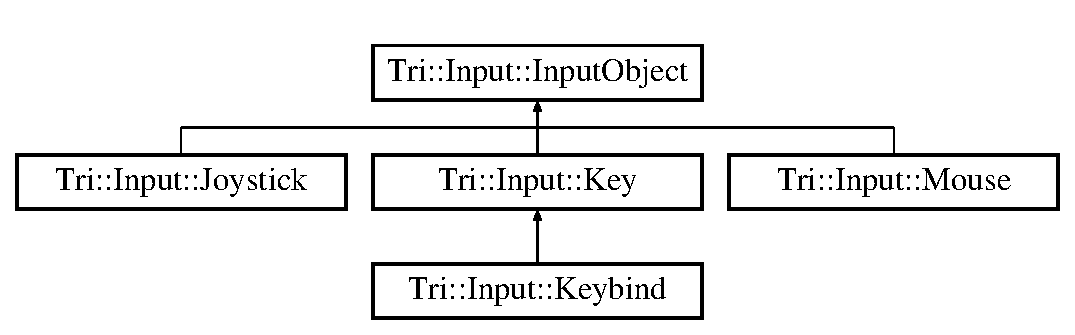
\includegraphics[height=3.000000cm]{class_tri_1_1_input_1_1_input_object}
\end{center}
\end{figure}
\subsection*{Friends}
\begin{DoxyCompactItemize}
\item 
class \hyperlink{class_tri_1_1_input_1_1_input_object_af0e8c3dcc20b7ddcaf63506363a22821}{Input\+Manager}
\end{DoxyCompactItemize}


\subsection{Detailed Description}


Definition at line 30 of file base.\+h.



\subsection{Friends And Related Function Documentation}
\hypertarget{class_tri_1_1_input_1_1_input_object_af0e8c3dcc20b7ddcaf63506363a22821}{}\index{Tri\+::\+Input\+::\+Input\+Object@{Tri\+::\+Input\+::\+Input\+Object}!Input\+Manager@{Input\+Manager}}
\index{Input\+Manager@{Input\+Manager}!Tri\+::\+Input\+::\+Input\+Object@{Tri\+::\+Input\+::\+Input\+Object}}
\subsubsection[{Input\+Manager}]{\setlength{\rightskip}{0pt plus 5cm}friend class {\bf Input\+Manager}\hspace{0.3cm}{\ttfamily [friend]}}\label{class_tri_1_1_input_1_1_input_object_af0e8c3dcc20b7ddcaf63506363a22821}


Definition at line 33 of file base.\+h.



The documentation for this class was generated from the following file\+:\begin{DoxyCompactItemize}
\item 
input/\hyperlink{base_8h}{base.\+h}\end{DoxyCompactItemize}

\hypertarget{class_tri_1_1_input_1_1_joystick}{}\section{Tri\+:\+:Input\+:\+:Joystick Class Reference}
\label{class_tri_1_1_input_1_1_joystick}\index{Tri\+::\+Input\+::\+Joystick@{Tri\+::\+Input\+::\+Joystick}}


{\ttfamily \#include $<$joystick.\+h$>$}

Inheritance diagram for Tri\+:\+:Input\+:\+:Joystick\+:\begin{figure}[H]
\begin{center}
\leavevmode
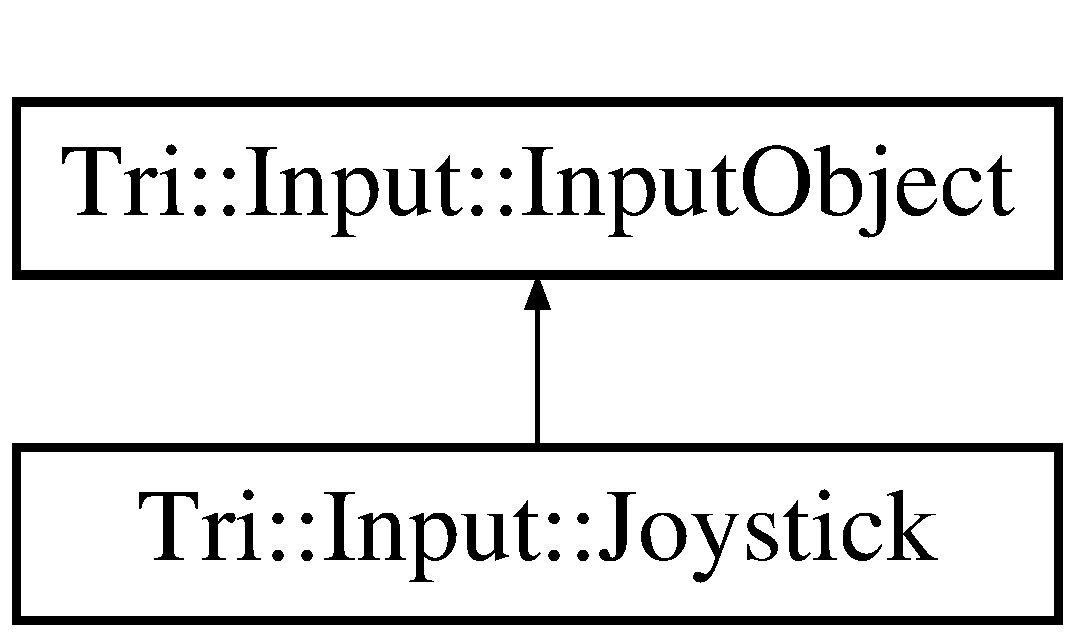
\includegraphics[height=2.000000cm]{class_tri_1_1_input_1_1_joystick}
\end{center}
\end{figure}
\subsection*{Public Types}
\begin{DoxyCompactItemize}
\item 
enum \hyperlink{class_tri_1_1_input_1_1_joystick_ae053177eed8f746c683d7bb9afc8dbb3}{Joystick\+Index} \{ \\*
\hyperlink{class_tri_1_1_input_1_1_joystick_ae053177eed8f746c683d7bb9afc8dbb3ae275d7e5ade8e9835c3b6c3563096260}{J\+O\+Y\+S\+T\+I\+C\+K\+\_\+1}, 
\hyperlink{class_tri_1_1_input_1_1_joystick_ae053177eed8f746c683d7bb9afc8dbb3a371f8ede5f041fecf96e733e986e0559}{J\+O\+Y\+S\+T\+I\+C\+K\+\_\+2}, 
\hyperlink{class_tri_1_1_input_1_1_joystick_ae053177eed8f746c683d7bb9afc8dbb3ac458a00f2e518cd7048f4f51a2a24a47}{J\+O\+Y\+S\+T\+I\+C\+K\+\_\+3}, 
\hyperlink{class_tri_1_1_input_1_1_joystick_ae053177eed8f746c683d7bb9afc8dbb3a9ae5166fa6b0aacf03d1fbed3b77794d}{J\+O\+Y\+S\+T\+I\+C\+K\+\_\+4}, 
\\*
\hyperlink{class_tri_1_1_input_1_1_joystick_ae053177eed8f746c683d7bb9afc8dbb3ada8aa493436ab2b3b0b289b390cbd668}{J\+O\+Y\+S\+T\+I\+C\+K\+\_\+5}, 
\hyperlink{class_tri_1_1_input_1_1_joystick_ae053177eed8f746c683d7bb9afc8dbb3a19a44263bbbb524aeff147f8bb960032}{J\+O\+Y\+S\+T\+I\+C\+K\+\_\+6}, 
\hyperlink{class_tri_1_1_input_1_1_joystick_ae053177eed8f746c683d7bb9afc8dbb3a5f287e3ce8834b5c6180ab53b1eb4247}{J\+O\+Y\+S\+T\+I\+C\+K\+\_\+7}, 
\hyperlink{class_tri_1_1_input_1_1_joystick_ae053177eed8f746c683d7bb9afc8dbb3a945c26dd6afb90b92aca8ed3ae59f1f5}{J\+O\+Y\+S\+T\+I\+C\+K\+\_\+8}, 
\\*
\hyperlink{class_tri_1_1_input_1_1_joystick_ae053177eed8f746c683d7bb9afc8dbb3ab467cddc3105048e68c456bac7313f3e}{J\+O\+Y\+S\+T\+I\+C\+K\+\_\+9}, 
\hyperlink{class_tri_1_1_input_1_1_joystick_ae053177eed8f746c683d7bb9afc8dbb3a36898030b78fedb30b6d976461570d7b}{J\+O\+Y\+S\+T\+I\+C\+K\+\_\+10}, 
\hyperlink{class_tri_1_1_input_1_1_joystick_ae053177eed8f746c683d7bb9afc8dbb3a020e6ccba9b9e1e91b8b5f7394e64c87}{J\+O\+Y\+S\+T\+I\+C\+K\+\_\+11}, 
\hyperlink{class_tri_1_1_input_1_1_joystick_ae053177eed8f746c683d7bb9afc8dbb3a2ef5ad8a23350cea09348981c9fe30c6}{J\+O\+Y\+S\+T\+I\+C\+K\+\_\+12}, 
\\*
\hyperlink{class_tri_1_1_input_1_1_joystick_ae053177eed8f746c683d7bb9afc8dbb3a651abf9dd96108376b50307cf885b275}{J\+O\+Y\+S\+T\+I\+C\+K\+\_\+13}, 
\hyperlink{class_tri_1_1_input_1_1_joystick_ae053177eed8f746c683d7bb9afc8dbb3ab7d72a4dbb5b859bb90390e742718950}{J\+O\+Y\+S\+T\+I\+C\+K\+\_\+14}, 
\hyperlink{class_tri_1_1_input_1_1_joystick_ae053177eed8f746c683d7bb9afc8dbb3a117825d42fa2d66416bd43ccb322397b}{J\+O\+Y\+S\+T\+I\+C\+K\+\_\+15}, 
\hyperlink{class_tri_1_1_input_1_1_joystick_ae053177eed8f746c683d7bb9afc8dbb3af9758a824d5c015e75da0a5fee0b1ef2}{J\+O\+Y\+S\+T\+I\+C\+K\+\_\+16}, 
\\*
\hyperlink{class_tri_1_1_input_1_1_joystick_ae053177eed8f746c683d7bb9afc8dbb3aa6ae366304a575777d1af63334af61fb}{J\+O\+Y\+S\+T\+I\+C\+K\+\_\+\+L\+A\+S\+T} = J\+O\+Y\+S\+T\+I\+C\+K\+\_\+16
 \}
\item 
typedef void($\ast$ \hyperlink{class_tri_1_1_input_1_1_joystick_adb19d991b2b53faf342e4497758d3764}{joystickcallfun}) (int, float $\ast$, int, \hyperlink{namespace_tri_1_1_input_1_1_system_a79600e9f4ed835251eed1706ce96bed0}{System\+::\+Action} $\ast$, int)
\begin{DoxyCompactList}\small\item\em The function signature for key callbacks. \end{DoxyCompactList}\end{DoxyCompactItemize}
\subsection*{Public Member Functions}
\begin{DoxyCompactItemize}
\item 
float \hyperlink{class_tri_1_1_input_1_1_joystick_a39d0488c1b8890593fe05aca340f55f5}{Get\+Joystick\+Position} (int index)
\item 
\hyperlink{namespace_tri_1_1_input_1_1_system_a79600e9f4ed835251eed1706ce96bed0}{System\+::\+Action} \hyperlink{class_tri_1_1_input_1_1_joystick_a0798e6984417aa7e4b87ffa20aa313f9}{Get\+Joystick\+Action} (int index)
\item 
Util\+::\+String \hyperlink{class_tri_1_1_input_1_1_joystick_aa5071d1361829912b7a70ad62fdc5f7b}{Get\+Name} ()
\item 
\hyperlink{class_tri_1_1_input_1_1_joystick_ae053177eed8f746c683d7bb9afc8dbb3}{Joystick\+Index} \hyperlink{class_tri_1_1_input_1_1_joystick_afec0add8c3e520e089cf18a52d131164}{Get\+Joystick\+Index} ()
\item 
void \hyperlink{class_tri_1_1_input_1_1_joystick_a3aec815dc3ccb5a5b91da00be6e91a16}{Set\+Joystick\+Callback} (\hyperlink{class_tri_1_1_input_1_1_joystick_adb19d991b2b53faf342e4497758d3764}{joystickcallfun} callback)
\item 
bool \hyperlink{class_tri_1_1_input_1_1_joystick_a5434131b363bf9af7d3e6f043eeda15a}{Is\+Joystick\+Index} (\hyperlink{class_tri_1_1_input_1_1_joystick_ae053177eed8f746c683d7bb9afc8dbb3}{Joystick\+Index} index)
\item 
bool \hyperlink{class_tri_1_1_input_1_1_joystick_a6ca63fab5af16061786d2752defee239}{Is\+Present} ()
\end{DoxyCompactItemize}
\subsection*{Protected Member Functions}
\begin{DoxyCompactItemize}
\item 
\hyperlink{class_tri_1_1_input_1_1_joystick_a2b9df8a7989454ead020526745d49fdb}{Joystick} (\hyperlink{class_tri_1_1_input_1_1_joystick_ae053177eed8f746c683d7bb9afc8dbb3}{Joystick\+Index} index)
\end{DoxyCompactItemize}
\subsection*{Protected Attributes}
\begin{DoxyCompactItemize}
\item 
float $\ast$ \hyperlink{class_tri_1_1_input_1_1_joystick_a572652754a153f3a63653768d1861c69}{m\+\_\+\+Joystick\+Position}
\item 
\hyperlink{namespace_tri_1_1_input_1_1_system_a79600e9f4ed835251eed1706ce96bed0}{System\+::\+Action} $\ast$ \hyperlink{class_tri_1_1_input_1_1_joystick_a01085701baf18c41dc10f9cf98d84562}{m\+\_\+\+Joystick\+Action}
\end{DoxyCompactItemize}


\subsection{Detailed Description}


Definition at line 10 of file joystick.\+h.



\subsection{Member Typedef Documentation}
\hypertarget{class_tri_1_1_input_1_1_joystick_adb19d991b2b53faf342e4497758d3764}{}\index{Tri\+::\+Input\+::\+Joystick@{Tri\+::\+Input\+::\+Joystick}!joystickcallfun@{joystickcallfun}}
\index{joystickcallfun@{joystickcallfun}!Tri\+::\+Input\+::\+Joystick@{Tri\+::\+Input\+::\+Joystick}}
\subsubsection[{joystickcallfun}]{\setlength{\rightskip}{0pt plus 5cm}typedef void($\ast$  Tri\+::\+Input\+::\+Joystick\+::joystickcallfun) (int, float $\ast$, int, {\bf System\+::\+Action} $\ast$, int)}\label{class_tri_1_1_input_1_1_joystick_adb19d991b2b53faf342e4497758d3764}


The function signature for key callbacks. 

The function signature for key callbacks for use with keybinds


\begin{DoxyParams}[1]{Parameters}
\mbox{\tt in}  & {\em axe\+Count} & The axe count for the array axes \\
\hline
\mbox{\tt in}  & {\em axes} & The array of axes with a length of axe\+Count \\
\hline
\mbox{\tt in}  & {\em button\+Count} & The button count for array buttons \\
\hline
\mbox{\tt in}  & {\em buttons} & The array of buttons with a length of button\+Count \\
\hline
\mbox{\tt in}  & {\em mods} & The current bit field modifier describing what modifier keys were held \\
\hline
\end{DoxyParams}


Definition at line 45 of file joystick.\+h.



\subsection{Member Enumeration Documentation}
\hypertarget{class_tri_1_1_input_1_1_joystick_ae053177eed8f746c683d7bb9afc8dbb3}{}\index{Tri\+::\+Input\+::\+Joystick@{Tri\+::\+Input\+::\+Joystick}!Joystick\+Index@{Joystick\+Index}}
\index{Joystick\+Index@{Joystick\+Index}!Tri\+::\+Input\+::\+Joystick@{Tri\+::\+Input\+::\+Joystick}}
\subsubsection[{Joystick\+Index}]{\setlength{\rightskip}{0pt plus 5cm}enum {\bf Tri\+::\+Input\+::\+Joystick\+::\+Joystick\+Index}}\label{class_tri_1_1_input_1_1_joystick_ae053177eed8f746c683d7bb9afc8dbb3}
\begin{Desc}
\item[Enumerator]\par
\begin{description}
\index{J\+O\+Y\+S\+T\+I\+C\+K\+\_\+1@{J\+O\+Y\+S\+T\+I\+C\+K\+\_\+1}!Tri\+::\+Input\+::\+Joystick@{Tri\+::\+Input\+::\+Joystick}}\index{Tri\+::\+Input\+::\+Joystick@{Tri\+::\+Input\+::\+Joystick}!J\+O\+Y\+S\+T\+I\+C\+K\+\_\+1@{J\+O\+Y\+S\+T\+I\+C\+K\+\_\+1}}\item[{\em 
\hypertarget{class_tri_1_1_input_1_1_joystick_ae053177eed8f746c683d7bb9afc8dbb3ae275d7e5ade8e9835c3b6c3563096260}{}J\+O\+Y\+S\+T\+I\+C\+K\+\_\+1\label{class_tri_1_1_input_1_1_joystick_ae053177eed8f746c683d7bb9afc8dbb3ae275d7e5ade8e9835c3b6c3563096260}
}]\index{J\+O\+Y\+S\+T\+I\+C\+K\+\_\+2@{J\+O\+Y\+S\+T\+I\+C\+K\+\_\+2}!Tri\+::\+Input\+::\+Joystick@{Tri\+::\+Input\+::\+Joystick}}\index{Tri\+::\+Input\+::\+Joystick@{Tri\+::\+Input\+::\+Joystick}!J\+O\+Y\+S\+T\+I\+C\+K\+\_\+2@{J\+O\+Y\+S\+T\+I\+C\+K\+\_\+2}}\item[{\em 
\hypertarget{class_tri_1_1_input_1_1_joystick_ae053177eed8f746c683d7bb9afc8dbb3a371f8ede5f041fecf96e733e986e0559}{}J\+O\+Y\+S\+T\+I\+C\+K\+\_\+2\label{class_tri_1_1_input_1_1_joystick_ae053177eed8f746c683d7bb9afc8dbb3a371f8ede5f041fecf96e733e986e0559}
}]\index{J\+O\+Y\+S\+T\+I\+C\+K\+\_\+3@{J\+O\+Y\+S\+T\+I\+C\+K\+\_\+3}!Tri\+::\+Input\+::\+Joystick@{Tri\+::\+Input\+::\+Joystick}}\index{Tri\+::\+Input\+::\+Joystick@{Tri\+::\+Input\+::\+Joystick}!J\+O\+Y\+S\+T\+I\+C\+K\+\_\+3@{J\+O\+Y\+S\+T\+I\+C\+K\+\_\+3}}\item[{\em 
\hypertarget{class_tri_1_1_input_1_1_joystick_ae053177eed8f746c683d7bb9afc8dbb3ac458a00f2e518cd7048f4f51a2a24a47}{}J\+O\+Y\+S\+T\+I\+C\+K\+\_\+3\label{class_tri_1_1_input_1_1_joystick_ae053177eed8f746c683d7bb9afc8dbb3ac458a00f2e518cd7048f4f51a2a24a47}
}]\index{J\+O\+Y\+S\+T\+I\+C\+K\+\_\+4@{J\+O\+Y\+S\+T\+I\+C\+K\+\_\+4}!Tri\+::\+Input\+::\+Joystick@{Tri\+::\+Input\+::\+Joystick}}\index{Tri\+::\+Input\+::\+Joystick@{Tri\+::\+Input\+::\+Joystick}!J\+O\+Y\+S\+T\+I\+C\+K\+\_\+4@{J\+O\+Y\+S\+T\+I\+C\+K\+\_\+4}}\item[{\em 
\hypertarget{class_tri_1_1_input_1_1_joystick_ae053177eed8f746c683d7bb9afc8dbb3a9ae5166fa6b0aacf03d1fbed3b77794d}{}J\+O\+Y\+S\+T\+I\+C\+K\+\_\+4\label{class_tri_1_1_input_1_1_joystick_ae053177eed8f746c683d7bb9afc8dbb3a9ae5166fa6b0aacf03d1fbed3b77794d}
}]\index{J\+O\+Y\+S\+T\+I\+C\+K\+\_\+5@{J\+O\+Y\+S\+T\+I\+C\+K\+\_\+5}!Tri\+::\+Input\+::\+Joystick@{Tri\+::\+Input\+::\+Joystick}}\index{Tri\+::\+Input\+::\+Joystick@{Tri\+::\+Input\+::\+Joystick}!J\+O\+Y\+S\+T\+I\+C\+K\+\_\+5@{J\+O\+Y\+S\+T\+I\+C\+K\+\_\+5}}\item[{\em 
\hypertarget{class_tri_1_1_input_1_1_joystick_ae053177eed8f746c683d7bb9afc8dbb3ada8aa493436ab2b3b0b289b390cbd668}{}J\+O\+Y\+S\+T\+I\+C\+K\+\_\+5\label{class_tri_1_1_input_1_1_joystick_ae053177eed8f746c683d7bb9afc8dbb3ada8aa493436ab2b3b0b289b390cbd668}
}]\index{J\+O\+Y\+S\+T\+I\+C\+K\+\_\+6@{J\+O\+Y\+S\+T\+I\+C\+K\+\_\+6}!Tri\+::\+Input\+::\+Joystick@{Tri\+::\+Input\+::\+Joystick}}\index{Tri\+::\+Input\+::\+Joystick@{Tri\+::\+Input\+::\+Joystick}!J\+O\+Y\+S\+T\+I\+C\+K\+\_\+6@{J\+O\+Y\+S\+T\+I\+C\+K\+\_\+6}}\item[{\em 
\hypertarget{class_tri_1_1_input_1_1_joystick_ae053177eed8f746c683d7bb9afc8dbb3a19a44263bbbb524aeff147f8bb960032}{}J\+O\+Y\+S\+T\+I\+C\+K\+\_\+6\label{class_tri_1_1_input_1_1_joystick_ae053177eed8f746c683d7bb9afc8dbb3a19a44263bbbb524aeff147f8bb960032}
}]\index{J\+O\+Y\+S\+T\+I\+C\+K\+\_\+7@{J\+O\+Y\+S\+T\+I\+C\+K\+\_\+7}!Tri\+::\+Input\+::\+Joystick@{Tri\+::\+Input\+::\+Joystick}}\index{Tri\+::\+Input\+::\+Joystick@{Tri\+::\+Input\+::\+Joystick}!J\+O\+Y\+S\+T\+I\+C\+K\+\_\+7@{J\+O\+Y\+S\+T\+I\+C\+K\+\_\+7}}\item[{\em 
\hypertarget{class_tri_1_1_input_1_1_joystick_ae053177eed8f746c683d7bb9afc8dbb3a5f287e3ce8834b5c6180ab53b1eb4247}{}J\+O\+Y\+S\+T\+I\+C\+K\+\_\+7\label{class_tri_1_1_input_1_1_joystick_ae053177eed8f746c683d7bb9afc8dbb3a5f287e3ce8834b5c6180ab53b1eb4247}
}]\index{J\+O\+Y\+S\+T\+I\+C\+K\+\_\+8@{J\+O\+Y\+S\+T\+I\+C\+K\+\_\+8}!Tri\+::\+Input\+::\+Joystick@{Tri\+::\+Input\+::\+Joystick}}\index{Tri\+::\+Input\+::\+Joystick@{Tri\+::\+Input\+::\+Joystick}!J\+O\+Y\+S\+T\+I\+C\+K\+\_\+8@{J\+O\+Y\+S\+T\+I\+C\+K\+\_\+8}}\item[{\em 
\hypertarget{class_tri_1_1_input_1_1_joystick_ae053177eed8f746c683d7bb9afc8dbb3a945c26dd6afb90b92aca8ed3ae59f1f5}{}J\+O\+Y\+S\+T\+I\+C\+K\+\_\+8\label{class_tri_1_1_input_1_1_joystick_ae053177eed8f746c683d7bb9afc8dbb3a945c26dd6afb90b92aca8ed3ae59f1f5}
}]\index{J\+O\+Y\+S\+T\+I\+C\+K\+\_\+9@{J\+O\+Y\+S\+T\+I\+C\+K\+\_\+9}!Tri\+::\+Input\+::\+Joystick@{Tri\+::\+Input\+::\+Joystick}}\index{Tri\+::\+Input\+::\+Joystick@{Tri\+::\+Input\+::\+Joystick}!J\+O\+Y\+S\+T\+I\+C\+K\+\_\+9@{J\+O\+Y\+S\+T\+I\+C\+K\+\_\+9}}\item[{\em 
\hypertarget{class_tri_1_1_input_1_1_joystick_ae053177eed8f746c683d7bb9afc8dbb3ab467cddc3105048e68c456bac7313f3e}{}J\+O\+Y\+S\+T\+I\+C\+K\+\_\+9\label{class_tri_1_1_input_1_1_joystick_ae053177eed8f746c683d7bb9afc8dbb3ab467cddc3105048e68c456bac7313f3e}
}]\index{J\+O\+Y\+S\+T\+I\+C\+K\+\_\+10@{J\+O\+Y\+S\+T\+I\+C\+K\+\_\+10}!Tri\+::\+Input\+::\+Joystick@{Tri\+::\+Input\+::\+Joystick}}\index{Tri\+::\+Input\+::\+Joystick@{Tri\+::\+Input\+::\+Joystick}!J\+O\+Y\+S\+T\+I\+C\+K\+\_\+10@{J\+O\+Y\+S\+T\+I\+C\+K\+\_\+10}}\item[{\em 
\hypertarget{class_tri_1_1_input_1_1_joystick_ae053177eed8f746c683d7bb9afc8dbb3a36898030b78fedb30b6d976461570d7b}{}J\+O\+Y\+S\+T\+I\+C\+K\+\_\+10\label{class_tri_1_1_input_1_1_joystick_ae053177eed8f746c683d7bb9afc8dbb3a36898030b78fedb30b6d976461570d7b}
}]\index{J\+O\+Y\+S\+T\+I\+C\+K\+\_\+11@{J\+O\+Y\+S\+T\+I\+C\+K\+\_\+11}!Tri\+::\+Input\+::\+Joystick@{Tri\+::\+Input\+::\+Joystick}}\index{Tri\+::\+Input\+::\+Joystick@{Tri\+::\+Input\+::\+Joystick}!J\+O\+Y\+S\+T\+I\+C\+K\+\_\+11@{J\+O\+Y\+S\+T\+I\+C\+K\+\_\+11}}\item[{\em 
\hypertarget{class_tri_1_1_input_1_1_joystick_ae053177eed8f746c683d7bb9afc8dbb3a020e6ccba9b9e1e91b8b5f7394e64c87}{}J\+O\+Y\+S\+T\+I\+C\+K\+\_\+11\label{class_tri_1_1_input_1_1_joystick_ae053177eed8f746c683d7bb9afc8dbb3a020e6ccba9b9e1e91b8b5f7394e64c87}
}]\index{J\+O\+Y\+S\+T\+I\+C\+K\+\_\+12@{J\+O\+Y\+S\+T\+I\+C\+K\+\_\+12}!Tri\+::\+Input\+::\+Joystick@{Tri\+::\+Input\+::\+Joystick}}\index{Tri\+::\+Input\+::\+Joystick@{Tri\+::\+Input\+::\+Joystick}!J\+O\+Y\+S\+T\+I\+C\+K\+\_\+12@{J\+O\+Y\+S\+T\+I\+C\+K\+\_\+12}}\item[{\em 
\hypertarget{class_tri_1_1_input_1_1_joystick_ae053177eed8f746c683d7bb9afc8dbb3a2ef5ad8a23350cea09348981c9fe30c6}{}J\+O\+Y\+S\+T\+I\+C\+K\+\_\+12\label{class_tri_1_1_input_1_1_joystick_ae053177eed8f746c683d7bb9afc8dbb3a2ef5ad8a23350cea09348981c9fe30c6}
}]\index{J\+O\+Y\+S\+T\+I\+C\+K\+\_\+13@{J\+O\+Y\+S\+T\+I\+C\+K\+\_\+13}!Tri\+::\+Input\+::\+Joystick@{Tri\+::\+Input\+::\+Joystick}}\index{Tri\+::\+Input\+::\+Joystick@{Tri\+::\+Input\+::\+Joystick}!J\+O\+Y\+S\+T\+I\+C\+K\+\_\+13@{J\+O\+Y\+S\+T\+I\+C\+K\+\_\+13}}\item[{\em 
\hypertarget{class_tri_1_1_input_1_1_joystick_ae053177eed8f746c683d7bb9afc8dbb3a651abf9dd96108376b50307cf885b275}{}J\+O\+Y\+S\+T\+I\+C\+K\+\_\+13\label{class_tri_1_1_input_1_1_joystick_ae053177eed8f746c683d7bb9afc8dbb3a651abf9dd96108376b50307cf885b275}
}]\index{J\+O\+Y\+S\+T\+I\+C\+K\+\_\+14@{J\+O\+Y\+S\+T\+I\+C\+K\+\_\+14}!Tri\+::\+Input\+::\+Joystick@{Tri\+::\+Input\+::\+Joystick}}\index{Tri\+::\+Input\+::\+Joystick@{Tri\+::\+Input\+::\+Joystick}!J\+O\+Y\+S\+T\+I\+C\+K\+\_\+14@{J\+O\+Y\+S\+T\+I\+C\+K\+\_\+14}}\item[{\em 
\hypertarget{class_tri_1_1_input_1_1_joystick_ae053177eed8f746c683d7bb9afc8dbb3ab7d72a4dbb5b859bb90390e742718950}{}J\+O\+Y\+S\+T\+I\+C\+K\+\_\+14\label{class_tri_1_1_input_1_1_joystick_ae053177eed8f746c683d7bb9afc8dbb3ab7d72a4dbb5b859bb90390e742718950}
}]\index{J\+O\+Y\+S\+T\+I\+C\+K\+\_\+15@{J\+O\+Y\+S\+T\+I\+C\+K\+\_\+15}!Tri\+::\+Input\+::\+Joystick@{Tri\+::\+Input\+::\+Joystick}}\index{Tri\+::\+Input\+::\+Joystick@{Tri\+::\+Input\+::\+Joystick}!J\+O\+Y\+S\+T\+I\+C\+K\+\_\+15@{J\+O\+Y\+S\+T\+I\+C\+K\+\_\+15}}\item[{\em 
\hypertarget{class_tri_1_1_input_1_1_joystick_ae053177eed8f746c683d7bb9afc8dbb3a117825d42fa2d66416bd43ccb322397b}{}J\+O\+Y\+S\+T\+I\+C\+K\+\_\+15\label{class_tri_1_1_input_1_1_joystick_ae053177eed8f746c683d7bb9afc8dbb3a117825d42fa2d66416bd43ccb322397b}
}]\index{J\+O\+Y\+S\+T\+I\+C\+K\+\_\+16@{J\+O\+Y\+S\+T\+I\+C\+K\+\_\+16}!Tri\+::\+Input\+::\+Joystick@{Tri\+::\+Input\+::\+Joystick}}\index{Tri\+::\+Input\+::\+Joystick@{Tri\+::\+Input\+::\+Joystick}!J\+O\+Y\+S\+T\+I\+C\+K\+\_\+16@{J\+O\+Y\+S\+T\+I\+C\+K\+\_\+16}}\item[{\em 
\hypertarget{class_tri_1_1_input_1_1_joystick_ae053177eed8f746c683d7bb9afc8dbb3af9758a824d5c015e75da0a5fee0b1ef2}{}J\+O\+Y\+S\+T\+I\+C\+K\+\_\+16\label{class_tri_1_1_input_1_1_joystick_ae053177eed8f746c683d7bb9afc8dbb3af9758a824d5c015e75da0a5fee0b1ef2}
}]\index{J\+O\+Y\+S\+T\+I\+C\+K\+\_\+\+L\+A\+S\+T@{J\+O\+Y\+S\+T\+I\+C\+K\+\_\+\+L\+A\+S\+T}!Tri\+::\+Input\+::\+Joystick@{Tri\+::\+Input\+::\+Joystick}}\index{Tri\+::\+Input\+::\+Joystick@{Tri\+::\+Input\+::\+Joystick}!J\+O\+Y\+S\+T\+I\+C\+K\+\_\+\+L\+A\+S\+T@{J\+O\+Y\+S\+T\+I\+C\+K\+\_\+\+L\+A\+S\+T}}\item[{\em 
\hypertarget{class_tri_1_1_input_1_1_joystick_ae053177eed8f746c683d7bb9afc8dbb3aa6ae366304a575777d1af63334af61fb}{}J\+O\+Y\+S\+T\+I\+C\+K\+\_\+\+L\+A\+S\+T\label{class_tri_1_1_input_1_1_joystick_ae053177eed8f746c683d7bb9afc8dbb3aa6ae366304a575777d1af63334af61fb}
}]\end{description}
\end{Desc}


Definition at line 14 of file joystick.\+h.



\subsection{Constructor \& Destructor Documentation}
\hypertarget{class_tri_1_1_input_1_1_joystick_a2b9df8a7989454ead020526745d49fdb}{}\index{Tri\+::\+Input\+::\+Joystick@{Tri\+::\+Input\+::\+Joystick}!Joystick@{Joystick}}
\index{Joystick@{Joystick}!Tri\+::\+Input\+::\+Joystick@{Tri\+::\+Input\+::\+Joystick}}
\subsubsection[{Joystick}]{\setlength{\rightskip}{0pt plus 5cm}Tri\+::\+Input\+::\+Joystick\+::\+Joystick (
\begin{DoxyParamCaption}
\item[{{\bf Joystick\+Index}}]{index}
\end{DoxyParamCaption}
)\hspace{0.3cm}{\ttfamily [protected]}}\label{class_tri_1_1_input_1_1_joystick_a2b9df8a7989454ead020526745d49fdb}


\subsection{Member Function Documentation}
\hypertarget{class_tri_1_1_input_1_1_joystick_a0798e6984417aa7e4b87ffa20aa313f9}{}\index{Tri\+::\+Input\+::\+Joystick@{Tri\+::\+Input\+::\+Joystick}!Get\+Joystick\+Action@{Get\+Joystick\+Action}}
\index{Get\+Joystick\+Action@{Get\+Joystick\+Action}!Tri\+::\+Input\+::\+Joystick@{Tri\+::\+Input\+::\+Joystick}}
\subsubsection[{Get\+Joystick\+Action}]{\setlength{\rightskip}{0pt plus 5cm}{\bf System\+::\+Action} Tri\+::\+Input\+::\+Joystick\+::\+Get\+Joystick\+Action (
\begin{DoxyParamCaption}
\item[{int}]{index}
\end{DoxyParamCaption}
)}\label{class_tri_1_1_input_1_1_joystick_a0798e6984417aa7e4b87ffa20aa313f9}
\hypertarget{class_tri_1_1_input_1_1_joystick_afec0add8c3e520e089cf18a52d131164}{}\index{Tri\+::\+Input\+::\+Joystick@{Tri\+::\+Input\+::\+Joystick}!Get\+Joystick\+Index@{Get\+Joystick\+Index}}
\index{Get\+Joystick\+Index@{Get\+Joystick\+Index}!Tri\+::\+Input\+::\+Joystick@{Tri\+::\+Input\+::\+Joystick}}
\subsubsection[{Get\+Joystick\+Index}]{\setlength{\rightskip}{0pt plus 5cm}{\bf Joystick\+Index} Tri\+::\+Input\+::\+Joystick\+::\+Get\+Joystick\+Index (
\begin{DoxyParamCaption}
{}
\end{DoxyParamCaption}
)}\label{class_tri_1_1_input_1_1_joystick_afec0add8c3e520e089cf18a52d131164}
\hypertarget{class_tri_1_1_input_1_1_joystick_a39d0488c1b8890593fe05aca340f55f5}{}\index{Tri\+::\+Input\+::\+Joystick@{Tri\+::\+Input\+::\+Joystick}!Get\+Joystick\+Position@{Get\+Joystick\+Position}}
\index{Get\+Joystick\+Position@{Get\+Joystick\+Position}!Tri\+::\+Input\+::\+Joystick@{Tri\+::\+Input\+::\+Joystick}}
\subsubsection[{Get\+Joystick\+Position}]{\setlength{\rightskip}{0pt plus 5cm}float Tri\+::\+Input\+::\+Joystick\+::\+Get\+Joystick\+Position (
\begin{DoxyParamCaption}
\item[{int}]{index}
\end{DoxyParamCaption}
)}\label{class_tri_1_1_input_1_1_joystick_a39d0488c1b8890593fe05aca340f55f5}
\hypertarget{class_tri_1_1_input_1_1_joystick_aa5071d1361829912b7a70ad62fdc5f7b}{}\index{Tri\+::\+Input\+::\+Joystick@{Tri\+::\+Input\+::\+Joystick}!Get\+Name@{Get\+Name}}
\index{Get\+Name@{Get\+Name}!Tri\+::\+Input\+::\+Joystick@{Tri\+::\+Input\+::\+Joystick}}
\subsubsection[{Get\+Name}]{\setlength{\rightskip}{0pt plus 5cm}Util\+::\+String Tri\+::\+Input\+::\+Joystick\+::\+Get\+Name (
\begin{DoxyParamCaption}
{}
\end{DoxyParamCaption}
)}\label{class_tri_1_1_input_1_1_joystick_aa5071d1361829912b7a70ad62fdc5f7b}
\hypertarget{class_tri_1_1_input_1_1_joystick_a5434131b363bf9af7d3e6f043eeda15a}{}\index{Tri\+::\+Input\+::\+Joystick@{Tri\+::\+Input\+::\+Joystick}!Is\+Joystick\+Index@{Is\+Joystick\+Index}}
\index{Is\+Joystick\+Index@{Is\+Joystick\+Index}!Tri\+::\+Input\+::\+Joystick@{Tri\+::\+Input\+::\+Joystick}}
\subsubsection[{Is\+Joystick\+Index}]{\setlength{\rightskip}{0pt plus 5cm}bool Tri\+::\+Input\+::\+Joystick\+::\+Is\+Joystick\+Index (
\begin{DoxyParamCaption}
\item[{{\bf Joystick\+Index}}]{index}
\end{DoxyParamCaption}
)}\label{class_tri_1_1_input_1_1_joystick_a5434131b363bf9af7d3e6f043eeda15a}
\hypertarget{class_tri_1_1_input_1_1_joystick_a6ca63fab5af16061786d2752defee239}{}\index{Tri\+::\+Input\+::\+Joystick@{Tri\+::\+Input\+::\+Joystick}!Is\+Present@{Is\+Present}}
\index{Is\+Present@{Is\+Present}!Tri\+::\+Input\+::\+Joystick@{Tri\+::\+Input\+::\+Joystick}}
\subsubsection[{Is\+Present}]{\setlength{\rightskip}{0pt plus 5cm}bool Tri\+::\+Input\+::\+Joystick\+::\+Is\+Present (
\begin{DoxyParamCaption}
{}
\end{DoxyParamCaption}
)}\label{class_tri_1_1_input_1_1_joystick_a6ca63fab5af16061786d2752defee239}
\hypertarget{class_tri_1_1_input_1_1_joystick_a3aec815dc3ccb5a5b91da00be6e91a16}{}\index{Tri\+::\+Input\+::\+Joystick@{Tri\+::\+Input\+::\+Joystick}!Set\+Joystick\+Callback@{Set\+Joystick\+Callback}}
\index{Set\+Joystick\+Callback@{Set\+Joystick\+Callback}!Tri\+::\+Input\+::\+Joystick@{Tri\+::\+Input\+::\+Joystick}}
\subsubsection[{Set\+Joystick\+Callback}]{\setlength{\rightskip}{0pt plus 5cm}void Tri\+::\+Input\+::\+Joystick\+::\+Set\+Joystick\+Callback (
\begin{DoxyParamCaption}
\item[{{\bf joystickcallfun}}]{callback}
\end{DoxyParamCaption}
)}\label{class_tri_1_1_input_1_1_joystick_a3aec815dc3ccb5a5b91da00be6e91a16}


\subsection{Member Data Documentation}
\hypertarget{class_tri_1_1_input_1_1_joystick_a01085701baf18c41dc10f9cf98d84562}{}\index{Tri\+::\+Input\+::\+Joystick@{Tri\+::\+Input\+::\+Joystick}!m\+\_\+\+Joystick\+Action@{m\+\_\+\+Joystick\+Action}}
\index{m\+\_\+\+Joystick\+Action@{m\+\_\+\+Joystick\+Action}!Tri\+::\+Input\+::\+Joystick@{Tri\+::\+Input\+::\+Joystick}}
\subsubsection[{m\+\_\+\+Joystick\+Action}]{\setlength{\rightskip}{0pt plus 5cm}{\bf System\+::\+Action}$\ast$ Tri\+::\+Input\+::\+Joystick\+::m\+\_\+\+Joystick\+Action\hspace{0.3cm}{\ttfamily [protected]}}\label{class_tri_1_1_input_1_1_joystick_a01085701baf18c41dc10f9cf98d84562}


Definition at line 56 of file joystick.\+h.

\hypertarget{class_tri_1_1_input_1_1_joystick_a572652754a153f3a63653768d1861c69}{}\index{Tri\+::\+Input\+::\+Joystick@{Tri\+::\+Input\+::\+Joystick}!m\+\_\+\+Joystick\+Position@{m\+\_\+\+Joystick\+Position}}
\index{m\+\_\+\+Joystick\+Position@{m\+\_\+\+Joystick\+Position}!Tri\+::\+Input\+::\+Joystick@{Tri\+::\+Input\+::\+Joystick}}
\subsubsection[{m\+\_\+\+Joystick\+Position}]{\setlength{\rightskip}{0pt plus 5cm}float$\ast$ Tri\+::\+Input\+::\+Joystick\+::m\+\_\+\+Joystick\+Position\hspace{0.3cm}{\ttfamily [protected]}}\label{class_tri_1_1_input_1_1_joystick_a572652754a153f3a63653768d1861c69}


Definition at line 55 of file joystick.\+h.



The documentation for this class was generated from the following file\+:\begin{DoxyCompactItemize}
\item 
input/\hyperlink{joystick_8h}{joystick.\+h}\end{DoxyCompactItemize}

\hypertarget{struct_tri_1_1_input_1_1_key}{}\section{Tri\+:\+:Input\+:\+:Key Struct Reference}
\label{struct_tri_1_1_input_1_1_key}\index{Tri\+::\+Input\+::\+Key@{Tri\+::\+Input\+::\+Key}}


{\ttfamily \#include $<$key.\+h$>$}

Inheritance diagram for Tri\+:\+:Input\+:\+:Key\+:\begin{figure}[H]
\begin{center}
\leavevmode
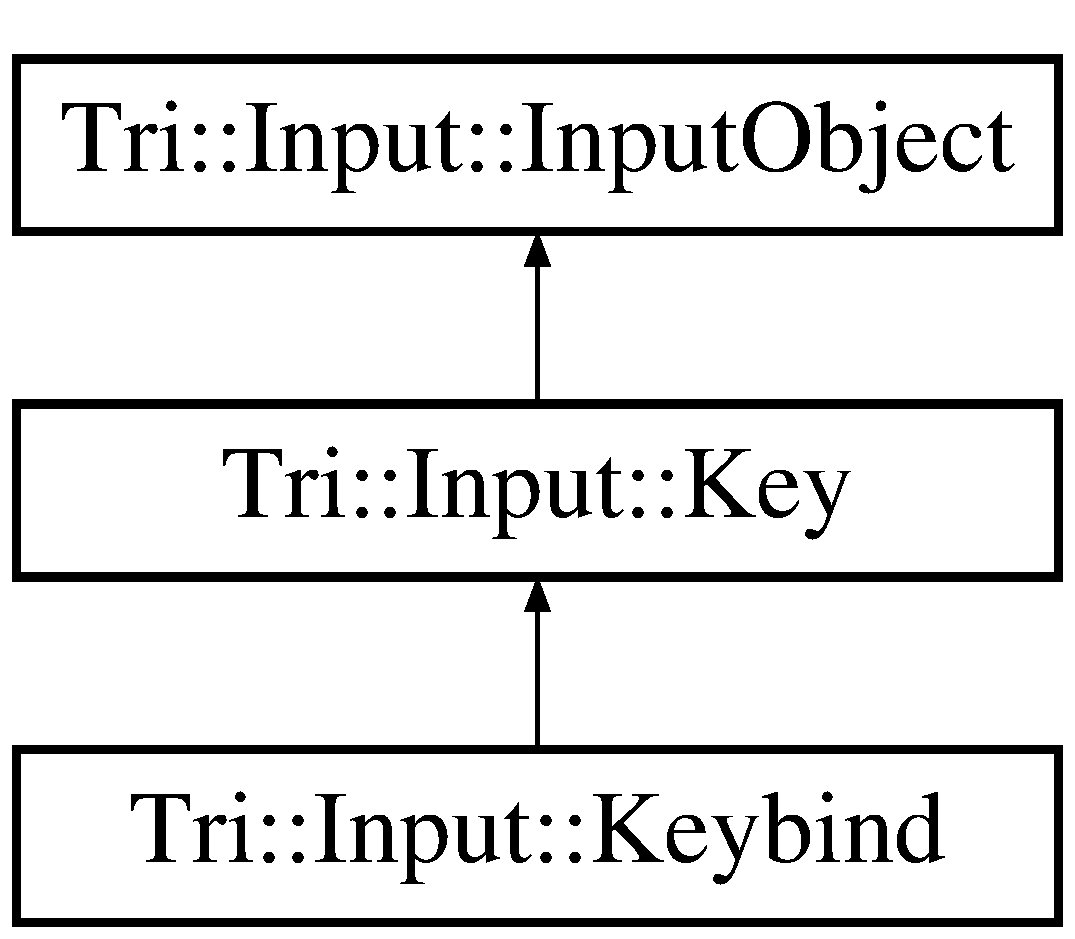
\includegraphics[height=3.000000cm]{struct_tri_1_1_input_1_1_key}
\end{center}
\end{figure}
\subsection*{Public Types}
\begin{DoxyCompactItemize}
\item 
enum \hyperlink{struct_tri_1_1_input_1_1_key_a0b1f54fb1b7be8fe2e920ca8552f86dc}{Key\+Index} \{ \\*
\hyperlink{struct_tri_1_1_input_1_1_key_a0b1f54fb1b7be8fe2e920ca8552f86dcab0f736b8851489d33839fc1fe5e3c13e}{U\+N\+K\+N\+O\+W\+N} = -\/1, 
\hyperlink{struct_tri_1_1_input_1_1_key_a0b1f54fb1b7be8fe2e920ca8552f86dca6c458c541c79ab0fcfb7f9820bbc02dc}{S\+P\+A\+C\+E} = 32, 
\hyperlink{struct_tri_1_1_input_1_1_key_a0b1f54fb1b7be8fe2e920ca8552f86dca118a41a9dcfc3d88f0a781cfdbedb3cb}{A\+P\+O\+S\+T\+R\+O\+P\+H\+E} = 39, 
\hyperlink{struct_tri_1_1_input_1_1_key_a0b1f54fb1b7be8fe2e920ca8552f86dca409b6cb304f84d89e9699e6c0a99a2cc}{C\+O\+M\+M\+A} = 44, 
\\*
\hyperlink{struct_tri_1_1_input_1_1_key_a0b1f54fb1b7be8fe2e920ca8552f86dcac1791accf259e853a4e99d956d0ea0bc}{M\+I\+N\+U\+S}, 
\hyperlink{struct_tri_1_1_input_1_1_key_a0b1f54fb1b7be8fe2e920ca8552f86dcabe3fa9e054cc572a0e530d482aabf3b1}{P\+E\+R\+I\+O\+D}, 
\hyperlink{struct_tri_1_1_input_1_1_key_a0b1f54fb1b7be8fe2e920ca8552f86dca74d731db64fc0bc0c0b913faed9e86c0}{S\+L\+A\+S\+H}, 
\hyperlink{struct_tri_1_1_input_1_1_key_a0b1f54fb1b7be8fe2e920ca8552f86dca190fdbc57ccc90259ee23265ca52ac36}{N\+U\+M\+\_\+0}, 
\\*
\hyperlink{struct_tri_1_1_input_1_1_key_a0b1f54fb1b7be8fe2e920ca8552f86dca25072a51ee799eba01b6bf03cb3ea076}{N\+U\+M\+\_\+1}, 
\hyperlink{struct_tri_1_1_input_1_1_key_a0b1f54fb1b7be8fe2e920ca8552f86dca1989313ee83e51e30f9fc63506262c2e}{N\+U\+M\+\_\+2}, 
\hyperlink{struct_tri_1_1_input_1_1_key_a0b1f54fb1b7be8fe2e920ca8552f86dca2779d3db32e4c6c3ed6e2dc919c2a456}{N\+U\+M\+\_\+3}, 
\hyperlink{struct_tri_1_1_input_1_1_key_a0b1f54fb1b7be8fe2e920ca8552f86dca9f5cb0d072b16932b5583569888720df}{N\+U\+M\+\_\+4}, 
\\*
\hyperlink{struct_tri_1_1_input_1_1_key_a0b1f54fb1b7be8fe2e920ca8552f86dca3d03e879073b1faf204838325ea662a0}{N\+U\+M\+\_\+5}, 
\hyperlink{struct_tri_1_1_input_1_1_key_a0b1f54fb1b7be8fe2e920ca8552f86dca9062d360f5e4b3baaa5b6f63fb94e7ce}{N\+U\+M\+\_\+6}, 
\hyperlink{struct_tri_1_1_input_1_1_key_a0b1f54fb1b7be8fe2e920ca8552f86dca41706d205751782728dd571b2d36a0c3}{N\+U\+M\+\_\+7}, 
\hyperlink{struct_tri_1_1_input_1_1_key_a0b1f54fb1b7be8fe2e920ca8552f86dca69401cd198a7cc63bc8c0486b68234c8}{N\+U\+M\+\_\+8}, 
\\*
\hyperlink{struct_tri_1_1_input_1_1_key_a0b1f54fb1b7be8fe2e920ca8552f86dca6d56b4d7728f8761e8e23d565e2c3236}{N\+U\+M\+\_\+9}, 
\hyperlink{struct_tri_1_1_input_1_1_key_a0b1f54fb1b7be8fe2e920ca8552f86dcabaaae16ed962711d8b4874cf5fa7f7e6}{S\+E\+M\+I\+C\+O\+L\+O\+N} = 59, 
\hyperlink{struct_tri_1_1_input_1_1_key_a0b1f54fb1b7be8fe2e920ca8552f86dcaf5d55b41283ec0099d41c2098d028bce}{E\+Q\+U\+A\+L} = 61, 
\hyperlink{struct_tri_1_1_input_1_1_key_a0b1f54fb1b7be8fe2e920ca8552f86dcab17ac11d12a69d29dfa74e2cc8efe438}{A} = 65, 
\\*
\hyperlink{struct_tri_1_1_input_1_1_key_a0b1f54fb1b7be8fe2e920ca8552f86dca00c4897bef6414ae497524b08dea1bc1}{B}, 
\hyperlink{struct_tri_1_1_input_1_1_key_a0b1f54fb1b7be8fe2e920ca8552f86dca5bef6708188281c7698c25eeca7372a0}{C}, 
\hyperlink{struct_tri_1_1_input_1_1_key_a0b1f54fb1b7be8fe2e920ca8552f86dca450a50984a6217116f6b899cccd896e8}{D}, 
\hyperlink{struct_tri_1_1_input_1_1_key_a0b1f54fb1b7be8fe2e920ca8552f86dcaa6eff8c644332ff429c68400eee49ec0}{E}, 
\\*
\hyperlink{struct_tri_1_1_input_1_1_key_a0b1f54fb1b7be8fe2e920ca8552f86dcab2ee5cbde10eb76cd60f0c3041d7170e}{F}, 
\hyperlink{struct_tri_1_1_input_1_1_key_a0b1f54fb1b7be8fe2e920ca8552f86dcad02d37780ffa1b6daf9edc8a96e34dfe}{G}, 
\hyperlink{struct_tri_1_1_input_1_1_key_a0b1f54fb1b7be8fe2e920ca8552f86dca904a0e5b5e9706df224ed10207f8a747}{H}, 
\hyperlink{struct_tri_1_1_input_1_1_key_a0b1f54fb1b7be8fe2e920ca8552f86dca28ca3f40ad1b93ee3f3006f517ca880d}{I}, 
\\*
\hyperlink{struct_tri_1_1_input_1_1_key_a0b1f54fb1b7be8fe2e920ca8552f86dca7eb9434b5db3e3a710ed650ea5a344b1}{J}, 
\hyperlink{struct_tri_1_1_input_1_1_key_a0b1f54fb1b7be8fe2e920ca8552f86dca5a6f40f9702d881d523c465490e5a947}{K}, 
\hyperlink{struct_tri_1_1_input_1_1_key_a0b1f54fb1b7be8fe2e920ca8552f86dca17e2ccb19766a8afb3d17430c8681ddb}{L}, 
\hyperlink{struct_tri_1_1_input_1_1_key_a0b1f54fb1b7be8fe2e920ca8552f86dcaec42c856e481b1457cf4adc03be00956}{M}, 
\\*
\hyperlink{struct_tri_1_1_input_1_1_key_a0b1f54fb1b7be8fe2e920ca8552f86dca89865fedb7e3dc9533489a555c3ca151}{N}, 
\hyperlink{struct_tri_1_1_input_1_1_key_a0b1f54fb1b7be8fe2e920ca8552f86dca461afe97571d3f758564d9a0cbcceb65}{O}, 
\hyperlink{struct_tri_1_1_input_1_1_key_a0b1f54fb1b7be8fe2e920ca8552f86dcae424e6a41939cd04992169099227bd10}{P}, 
\hyperlink{struct_tri_1_1_input_1_1_key_a0b1f54fb1b7be8fe2e920ca8552f86dcaf590a642bf82d61002749b83fc6f99a8}{Q}, 
\\*
\hyperlink{struct_tri_1_1_input_1_1_key_a0b1f54fb1b7be8fe2e920ca8552f86dcad8d90ac39df9a351819936dd0bf77bd8}{R}, 
\hyperlink{struct_tri_1_1_input_1_1_key_a0b1f54fb1b7be8fe2e920ca8552f86dca361ac2deb14096d8af3c0ddbd6d901f7}{S}, 
\hyperlink{struct_tri_1_1_input_1_1_key_a0b1f54fb1b7be8fe2e920ca8552f86dcab73d4a03ec6dea7a41a99abeb195daf7}{T}, 
\hyperlink{struct_tri_1_1_input_1_1_key_a0b1f54fb1b7be8fe2e920ca8552f86dcae8687ed03b8bf28b4c9bdde0c4db7fdd}{U}, 
\\*
\hyperlink{struct_tri_1_1_input_1_1_key_a0b1f54fb1b7be8fe2e920ca8552f86dca666fe29ef0f8e2f2b3744296923639e0}{V}, 
\hyperlink{struct_tri_1_1_input_1_1_key_a0b1f54fb1b7be8fe2e920ca8552f86dca0d9d402e40185723915aa1a904f9afc0}{W}, 
\hyperlink{struct_tri_1_1_input_1_1_key_a0b1f54fb1b7be8fe2e920ca8552f86dcab5305e1137768fce31bb831acb04a407}{X}, 
\hyperlink{struct_tri_1_1_input_1_1_key_a0b1f54fb1b7be8fe2e920ca8552f86dcaced54179bb2c1be16dab783d3911bfad}{Y}, 
\\*
\hyperlink{struct_tri_1_1_input_1_1_key_a0b1f54fb1b7be8fe2e920ca8552f86dcabfe87591a37dbd5f120233e69c70678d}{Z}, 
\hyperlink{struct_tri_1_1_input_1_1_key_a0b1f54fb1b7be8fe2e920ca8552f86dca671efbcd1567a211b0a75de5cdf7a061}{L\+E\+F\+T\+\_\+\+B\+R\+A\+C\+K\+E\+T}, 
\hyperlink{struct_tri_1_1_input_1_1_key_a0b1f54fb1b7be8fe2e920ca8552f86dca8c3f8d5e9a800f92c4417cbc93d12346}{B\+A\+C\+K\+S\+L\+A\+S\+H}, 
\hyperlink{struct_tri_1_1_input_1_1_key_a0b1f54fb1b7be8fe2e920ca8552f86dca9afbfeab294a3bfcf030279042c3d006}{R\+I\+G\+H\+T\+\_\+\+B\+R\+A\+C\+K\+E\+T}, 
\\*
\hyperlink{struct_tri_1_1_input_1_1_key_a0b1f54fb1b7be8fe2e920ca8552f86dcafa30413da4d576ea34b28652e79e0a93}{G\+R\+A\+V\+E\+\_\+\+A\+C\+C\+E\+N\+T} = 96, 
\hyperlink{struct_tri_1_1_input_1_1_key_a0b1f54fb1b7be8fe2e920ca8552f86dca5d53747f8cda356322dcf9eac435d6fb}{W\+O\+R\+L\+D\+\_\+1} = 161, 
\hyperlink{struct_tri_1_1_input_1_1_key_a0b1f54fb1b7be8fe2e920ca8552f86dcae7760e131028fd9dbc1405f9b79c2921}{W\+O\+R\+L\+D\+\_\+2}, 
\hyperlink{struct_tri_1_1_input_1_1_key_a0b1f54fb1b7be8fe2e920ca8552f86dca0fd6503e4d92e7b74ed9b29482dc65e5}{E\+S\+C\+A\+P\+E} = 256, 
\\*
\hyperlink{struct_tri_1_1_input_1_1_key_a0b1f54fb1b7be8fe2e920ca8552f86dca7ec1e437260b87bd74345da18016f2f1}{E\+N\+T\+E\+R}, 
\hyperlink{struct_tri_1_1_input_1_1_key_a0b1f54fb1b7be8fe2e920ca8552f86dcacfb7d695e46abb85d47aed67fdc1b901}{T\+A\+B}, 
\hyperlink{struct_tri_1_1_input_1_1_key_a0b1f54fb1b7be8fe2e920ca8552f86dcafe24ed9e1cc13825b153e6595ce5e185}{B\+A\+C\+K\+S\+P\+A\+C\+E}, 
\hyperlink{struct_tri_1_1_input_1_1_key_a0b1f54fb1b7be8fe2e920ca8552f86dca8ea6a343951255e25f305635e44189ea}{I\+N\+S\+E\+R\+T}, 
\\*
\hyperlink{struct_tri_1_1_input_1_1_key_a0b1f54fb1b7be8fe2e920ca8552f86dcad38bbd2e6e63d4c4e368ae4ef45c1e75}{D\+E\+L\+E\+T\+E}, 
\hyperlink{struct_tri_1_1_input_1_1_key_a0b1f54fb1b7be8fe2e920ca8552f86dca695af059009cb32214f406459cf0b37e}{R\+I\+G\+H\+T}, 
\hyperlink{struct_tri_1_1_input_1_1_key_a0b1f54fb1b7be8fe2e920ca8552f86dca52495a84c19aa17feffb6737841d66c1}{L\+E\+F\+T}, 
\hyperlink{struct_tri_1_1_input_1_1_key_a0b1f54fb1b7be8fe2e920ca8552f86dca22f20d98673440cacdef25d7c03e57f6}{D\+O\+W\+N}, 
\\*
\hyperlink{struct_tri_1_1_input_1_1_key_a0b1f54fb1b7be8fe2e920ca8552f86dca97af3b218ff03fb91ac09e03f1cea12a}{U\+P}, 
\hyperlink{struct_tri_1_1_input_1_1_key_a0b1f54fb1b7be8fe2e920ca8552f86dca48dd183030de83e70d9c94429768509a}{P\+A\+G\+E\+\_\+\+U\+P}, 
\hyperlink{struct_tri_1_1_input_1_1_key_a0b1f54fb1b7be8fe2e920ca8552f86dca216ceb75da508d63cf2dfb228b3817fb}{P\+A\+G\+E\+\_\+\+D\+O\+W\+N}, 
\hyperlink{struct_tri_1_1_input_1_1_key_a0b1f54fb1b7be8fe2e920ca8552f86dca6ab7e2615ed04122e346b8a4d428a4b5}{H\+O\+M\+E}, 
\\*
\hyperlink{struct_tri_1_1_input_1_1_key_a0b1f54fb1b7be8fe2e920ca8552f86dca6329b1f768b65ab7306822d99c027b4f}{E\+N\+D}, 
\hyperlink{struct_tri_1_1_input_1_1_key_a0b1f54fb1b7be8fe2e920ca8552f86dca798e1b2da8282e3387ba828e230dddf1}{C\+A\+P\+S\+\_\+\+L\+O\+C\+K} = 280, 
\hyperlink{struct_tri_1_1_input_1_1_key_a0b1f54fb1b7be8fe2e920ca8552f86dcabdedecf0e32658692ff3802c92c54feb}{S\+C\+R\+O\+L\+L\+\_\+\+L\+O\+C\+K}, 
\hyperlink{struct_tri_1_1_input_1_1_key_a0b1f54fb1b7be8fe2e920ca8552f86dca282a5c6c17bc0d6f7150352a1e75e9e2}{N\+U\+M\+\_\+\+L\+O\+C\+K}, 
\\*
\hyperlink{struct_tri_1_1_input_1_1_key_a0b1f54fb1b7be8fe2e920ca8552f86dcab9681d954f3c4f4805c4e2f4a6421929}{P\+R\+I\+N\+T\+\_\+\+S\+C\+R\+E\+E\+N}, 
\hyperlink{struct_tri_1_1_input_1_1_key_a0b1f54fb1b7be8fe2e920ca8552f86dca85541ac9f5c4053656b05987b90895e2}{P\+A\+U\+S\+E}, 
\hyperlink{struct_tri_1_1_input_1_1_key_a0b1f54fb1b7be8fe2e920ca8552f86dca0a92a13a460932576e18d90fa429c6b4}{F1} = 290, 
\hyperlink{struct_tri_1_1_input_1_1_key_a0b1f54fb1b7be8fe2e920ca8552f86dca6827a3c1b000ddf8a0e6a11822534c64}{F2}, 
\\*
\hyperlink{struct_tri_1_1_input_1_1_key_a0b1f54fb1b7be8fe2e920ca8552f86dca3a30ec221428eadbdfd230a98702244b}{F3}, 
\hyperlink{struct_tri_1_1_input_1_1_key_a0b1f54fb1b7be8fe2e920ca8552f86dca8cc6f3e196f31eb13687dbd5a27cdcfc}{F4}, 
\hyperlink{struct_tri_1_1_input_1_1_key_a0b1f54fb1b7be8fe2e920ca8552f86dcaa854cdd6e3f2f043a102ce3b73ff1793}{F5}, 
\hyperlink{struct_tri_1_1_input_1_1_key_a0b1f54fb1b7be8fe2e920ca8552f86dca7c230550b2eec236f7802a4b7ec9ff9d}{F6}, 
\\*
\hyperlink{struct_tri_1_1_input_1_1_key_a0b1f54fb1b7be8fe2e920ca8552f86dca8d8b5364274d0bf95819120e555fc38e}{F7}, 
\hyperlink{struct_tri_1_1_input_1_1_key_a0b1f54fb1b7be8fe2e920ca8552f86dca1f10748232eacd1fbb39e6355326ea3e}{F8}, 
\hyperlink{struct_tri_1_1_input_1_1_key_a0b1f54fb1b7be8fe2e920ca8552f86dcae2025c8c6580275af2c29e14d07b9fe2}{F9}, 
\hyperlink{struct_tri_1_1_input_1_1_key_a0b1f54fb1b7be8fe2e920ca8552f86dcaba5abbea3938458156a30713cd7a54a9}{F10}, 
\\*
\hyperlink{struct_tri_1_1_input_1_1_key_a0b1f54fb1b7be8fe2e920ca8552f86dca39bcc6c39af05a2b50809a5000caad7a}{F11}, 
\hyperlink{struct_tri_1_1_input_1_1_key_a0b1f54fb1b7be8fe2e920ca8552f86dca782e4ff975dedbd55760cbefe7ec9fea}{F12}, 
\hyperlink{struct_tri_1_1_input_1_1_key_a0b1f54fb1b7be8fe2e920ca8552f86dca62a720d960d86d69857c518dbf21eda3}{F13}, 
\hyperlink{struct_tri_1_1_input_1_1_key_a0b1f54fb1b7be8fe2e920ca8552f86dca7d4c02f5a509fe403cad708b2d4d8850}{F14}, 
\\*
\hyperlink{struct_tri_1_1_input_1_1_key_a0b1f54fb1b7be8fe2e920ca8552f86dca704323854c894953002eed62761181f3}{F15}, 
\hyperlink{struct_tri_1_1_input_1_1_key_a0b1f54fb1b7be8fe2e920ca8552f86dcae7db45455f4e22e0cdb03a6ff20d4f1b}{F16}, 
\hyperlink{struct_tri_1_1_input_1_1_key_a0b1f54fb1b7be8fe2e920ca8552f86dca4b94049c911eb3f5b9553c4117bd9771}{F17}, 
\hyperlink{struct_tri_1_1_input_1_1_key_a0b1f54fb1b7be8fe2e920ca8552f86dca7be89c4c9b55d055b6e03602659ed8cc}{F18}, 
\\*
\hyperlink{struct_tri_1_1_input_1_1_key_a0b1f54fb1b7be8fe2e920ca8552f86dca44a34007a82561be5b85a5f4ed2b5d1a}{F19}, 
\hyperlink{struct_tri_1_1_input_1_1_key_a0b1f54fb1b7be8fe2e920ca8552f86dca7fe38f0d3c85d71bb5e55a06c79cc3eb}{F20}, 
\hyperlink{struct_tri_1_1_input_1_1_key_a0b1f54fb1b7be8fe2e920ca8552f86dca791d0018b86d3fc2a124fc5b1c907bc1}{F21}, 
\hyperlink{struct_tri_1_1_input_1_1_key_a0b1f54fb1b7be8fe2e920ca8552f86dca83980a37ffff914f81408934943912ff}{F22}, 
\\*
\hyperlink{struct_tri_1_1_input_1_1_key_a0b1f54fb1b7be8fe2e920ca8552f86dcaf54b3b76b15a60cda71617414a8fed75}{F23}, 
\hyperlink{struct_tri_1_1_input_1_1_key_a0b1f54fb1b7be8fe2e920ca8552f86dca663b085f950773687233d9ea901c131a}{F24}, 
\hyperlink{struct_tri_1_1_input_1_1_key_a0b1f54fb1b7be8fe2e920ca8552f86dca517292e85e578065f585b86e8d291a76}{F25}, 
\hyperlink{struct_tri_1_1_input_1_1_key_a0b1f54fb1b7be8fe2e920ca8552f86dca8142095bd52e730df01f68e73f2a96b3}{K\+P\+\_\+0} = 320, 
\\*
\hyperlink{struct_tri_1_1_input_1_1_key_a0b1f54fb1b7be8fe2e920ca8552f86dca7b25add8f06a03aa45511bd4eefb8415}{K\+P\+\_\+1}, 
\hyperlink{struct_tri_1_1_input_1_1_key_a0b1f54fb1b7be8fe2e920ca8552f86dcacda9206dac17acbb8f82fb4540a605ab}{K\+P\+\_\+2}, 
\hyperlink{struct_tri_1_1_input_1_1_key_a0b1f54fb1b7be8fe2e920ca8552f86dcab7a0dab76d842ceca73a4a16345e5af6}{K\+P\+\_\+3}, 
\hyperlink{struct_tri_1_1_input_1_1_key_a0b1f54fb1b7be8fe2e920ca8552f86dca0cc520dcac0555bd7658b53b8dea8edc}{K\+P\+\_\+4}, 
\\*
\hyperlink{struct_tri_1_1_input_1_1_key_a0b1f54fb1b7be8fe2e920ca8552f86dcaba969d55e89c93eb9e350cf1fe54842a}{K\+P\+\_\+5}, 
\hyperlink{struct_tri_1_1_input_1_1_key_a0b1f54fb1b7be8fe2e920ca8552f86dcae07fcb853ddf6ff43f56796142a043c6}{K\+P\+\_\+6}, 
\hyperlink{struct_tri_1_1_input_1_1_key_a0b1f54fb1b7be8fe2e920ca8552f86dcaf8394acaea423fedf164813c7c36726e}{K\+P\+\_\+7}, 
\hyperlink{struct_tri_1_1_input_1_1_key_a0b1f54fb1b7be8fe2e920ca8552f86dca629be3f71be3f6be036bcaa10b4593a3}{K\+P\+\_\+8}, 
\\*
\hyperlink{struct_tri_1_1_input_1_1_key_a0b1f54fb1b7be8fe2e920ca8552f86dcacf0641577b91f3e3a31739a5e696e895}{K\+P\+\_\+9}, 
\hyperlink{struct_tri_1_1_input_1_1_key_a0b1f54fb1b7be8fe2e920ca8552f86dca629eec8cd3718cc46e3356ac90019c6e}{K\+P\+\_\+\+D\+E\+C\+I\+M\+A\+L}, 
\hyperlink{struct_tri_1_1_input_1_1_key_a0b1f54fb1b7be8fe2e920ca8552f86dca593bb999e7b8bdc9159521150a742d99}{K\+P\+\_\+\+D\+I\+V\+I\+D\+E}, 
\hyperlink{struct_tri_1_1_input_1_1_key_a0b1f54fb1b7be8fe2e920ca8552f86dca2d693c821e53c3bd0f8572b59baaa207}{K\+P\+\_\+\+M\+U\+L\+T\+I\+P\+L\+Y}, 
\\*
\hyperlink{struct_tri_1_1_input_1_1_key_a0b1f54fb1b7be8fe2e920ca8552f86dcaec9776c268b788b14a139b459f28ff00}{K\+P\+\_\+\+S\+U\+B\+T\+R\+A\+C\+T}, 
\hyperlink{struct_tri_1_1_input_1_1_key_a0b1f54fb1b7be8fe2e920ca8552f86dca5d0123937646d9db30453466e349f9b7}{K\+P\+\_\+\+A\+D\+D}, 
\hyperlink{struct_tri_1_1_input_1_1_key_a0b1f54fb1b7be8fe2e920ca8552f86dcabbb21fdf5eb9b4d9eaf9351a59639035}{K\+P\+\_\+\+E\+N\+T\+E\+R}, 
\hyperlink{struct_tri_1_1_input_1_1_key_a0b1f54fb1b7be8fe2e920ca8552f86dcaa01cc94fd57eb6a8d7f2294db22fe7fc}{K\+P\+\_\+\+E\+Q\+U\+A\+L}, 
\\*
\hyperlink{struct_tri_1_1_input_1_1_key_a0b1f54fb1b7be8fe2e920ca8552f86dcafd5d266d8e6d6e1177de849e71c33aad}{L\+E\+F\+T\+\_\+\+S\+H\+I\+F\+T} = 340, 
\hyperlink{struct_tri_1_1_input_1_1_key_a0b1f54fb1b7be8fe2e920ca8552f86dca0a5a186dbdb073ad278449392002f76b}{L\+E\+F\+T\+\_\+\+C\+O\+N\+T\+R\+O\+L}, 
\hyperlink{struct_tri_1_1_input_1_1_key_a0b1f54fb1b7be8fe2e920ca8552f86dcac6eaeb9128977fb11cb30fbcdfa92dd6}{L\+E\+F\+T\+\_\+\+A\+L\+T}, 
\hyperlink{struct_tri_1_1_input_1_1_key_a0b1f54fb1b7be8fe2e920ca8552f86dcae02f99237fcace4908178a9160cf6242}{L\+E\+F\+T\+\_\+\+S\+U\+P\+E\+R}, 
\\*
\hyperlink{struct_tri_1_1_input_1_1_key_a0b1f54fb1b7be8fe2e920ca8552f86dca032394c4fcdee54490e22efbb22a4f5f}{R\+I\+G\+H\+T\+\_\+\+S\+H\+I\+F\+T}, 
\hyperlink{struct_tri_1_1_input_1_1_key_a0b1f54fb1b7be8fe2e920ca8552f86dca6f37fc608ba167a583d31c756e8bb107}{R\+I\+G\+H\+T\+\_\+\+C\+O\+N\+T\+R\+O\+L}, 
\hyperlink{struct_tri_1_1_input_1_1_key_a0b1f54fb1b7be8fe2e920ca8552f86dcaf37b840ac60dce0be1c990eae1bb9eda}{R\+I\+G\+H\+T\+\_\+\+A\+L\+T}, 
\hyperlink{struct_tri_1_1_input_1_1_key_a0b1f54fb1b7be8fe2e920ca8552f86dca321842ee6c262a9a53f2110d554dab08}{R\+I\+G\+H\+T\+\_\+\+S\+U\+P\+E\+R}, 
\\*
\hyperlink{struct_tri_1_1_input_1_1_key_a0b1f54fb1b7be8fe2e920ca8552f86dca65441516d40860617d323c4e7b6ec02e}{M\+E\+N\+U}, 
\hyperlink{struct_tri_1_1_input_1_1_key_a0b1f54fb1b7be8fe2e920ca8552f86dcac355bc1545ddb8a555c1c19f7dc3ddec}{L\+A\+S\+T} = M\+E\+N\+U
 \}
\end{DoxyCompactItemize}
\subsection*{Public Member Functions}
\begin{DoxyCompactItemize}
\item 
\hyperlink{namespace_tri_1_1_input_1_1_system_a79600e9f4ed835251eed1706ce96bed0}{System\+::\+Action} \hyperlink{struct_tri_1_1_input_1_1_key_aab0d0353660113e5c32ebaf784378610}{Get\+Action} ()
\item 
\hyperlink{struct_tri_1_1_input_1_1_key_a0b1f54fb1b7be8fe2e920ca8552f86dc}{Key\+Index} \hyperlink{struct_tri_1_1_input_1_1_key_a3b4f39428b275aefb07f0f63421fdb84}{Get\+Key} ()
\item 
bool \hyperlink{struct_tri_1_1_input_1_1_key_a5729e09cefd10667decab7dae4130c10}{Is\+Pressed} ()
\item 
bool \hyperlink{struct_tri_1_1_input_1_1_key_a750cdcbd3177f25b8845b1142e590952}{Is\+Key} (\hyperlink{struct_tri_1_1_input_1_1_key_a0b1f54fb1b7be8fe2e920ca8552f86dc}{Key\+Index} index)
\end{DoxyCompactItemize}
\subsection*{Protected Member Functions}
\begin{DoxyCompactItemize}
\item 
\hyperlink{struct_tri_1_1_input_1_1_key_aa813871e191ce89ca9693207c3f9f063}{Key} (\hyperlink{struct_tri_1_1_input_1_1_key_a0b1f54fb1b7be8fe2e920ca8552f86dc}{Key\+Index} index)
\end{DoxyCompactItemize}
\subsection*{Protected Attributes}
\begin{DoxyCompactItemize}
\item 
\hyperlink{namespace_tri_1_1_input_1_1_system_a79600e9f4ed835251eed1706ce96bed0}{System\+::\+Action} $\ast$ \hyperlink{struct_tri_1_1_input_1_1_key_a4118499d9e3680859c603e1f70a2bcc3}{m\+\_\+\+Action}
\end{DoxyCompactItemize}


\subsection{Detailed Description}


Definition at line 10 of file key.\+h.



\subsection{Member Enumeration Documentation}
\hypertarget{struct_tri_1_1_input_1_1_key_a0b1f54fb1b7be8fe2e920ca8552f86dc}{}\index{Tri\+::\+Input\+::\+Key@{Tri\+::\+Input\+::\+Key}!Key\+Index@{Key\+Index}}
\index{Key\+Index@{Key\+Index}!Tri\+::\+Input\+::\+Key@{Tri\+::\+Input\+::\+Key}}
\subsubsection[{Key\+Index}]{\setlength{\rightskip}{0pt plus 5cm}enum {\bf Tri\+::\+Input\+::\+Key\+::\+Key\+Index}}\label{struct_tri_1_1_input_1_1_key_a0b1f54fb1b7be8fe2e920ca8552f86dc}
\begin{Desc}
\item[Enumerator]\par
\begin{description}
\index{U\+N\+K\+N\+O\+W\+N@{U\+N\+K\+N\+O\+W\+N}!Tri\+::\+Input\+::\+Key@{Tri\+::\+Input\+::\+Key}}\index{Tri\+::\+Input\+::\+Key@{Tri\+::\+Input\+::\+Key}!U\+N\+K\+N\+O\+W\+N@{U\+N\+K\+N\+O\+W\+N}}\item[{\em 
\hypertarget{struct_tri_1_1_input_1_1_key_a0b1f54fb1b7be8fe2e920ca8552f86dcab0f736b8851489d33839fc1fe5e3c13e}{}U\+N\+K\+N\+O\+W\+N\label{struct_tri_1_1_input_1_1_key_a0b1f54fb1b7be8fe2e920ca8552f86dcab0f736b8851489d33839fc1fe5e3c13e}
}]\index{S\+P\+A\+C\+E@{S\+P\+A\+C\+E}!Tri\+::\+Input\+::\+Key@{Tri\+::\+Input\+::\+Key}}\index{Tri\+::\+Input\+::\+Key@{Tri\+::\+Input\+::\+Key}!S\+P\+A\+C\+E@{S\+P\+A\+C\+E}}\item[{\em 
\hypertarget{struct_tri_1_1_input_1_1_key_a0b1f54fb1b7be8fe2e920ca8552f86dca6c458c541c79ab0fcfb7f9820bbc02dc}{}S\+P\+A\+C\+E\label{struct_tri_1_1_input_1_1_key_a0b1f54fb1b7be8fe2e920ca8552f86dca6c458c541c79ab0fcfb7f9820bbc02dc}
}]\index{A\+P\+O\+S\+T\+R\+O\+P\+H\+E@{A\+P\+O\+S\+T\+R\+O\+P\+H\+E}!Tri\+::\+Input\+::\+Key@{Tri\+::\+Input\+::\+Key}}\index{Tri\+::\+Input\+::\+Key@{Tri\+::\+Input\+::\+Key}!A\+P\+O\+S\+T\+R\+O\+P\+H\+E@{A\+P\+O\+S\+T\+R\+O\+P\+H\+E}}\item[{\em 
\hypertarget{struct_tri_1_1_input_1_1_key_a0b1f54fb1b7be8fe2e920ca8552f86dca118a41a9dcfc3d88f0a781cfdbedb3cb}{}A\+P\+O\+S\+T\+R\+O\+P\+H\+E\label{struct_tri_1_1_input_1_1_key_a0b1f54fb1b7be8fe2e920ca8552f86dca118a41a9dcfc3d88f0a781cfdbedb3cb}
}]\index{C\+O\+M\+M\+A@{C\+O\+M\+M\+A}!Tri\+::\+Input\+::\+Key@{Tri\+::\+Input\+::\+Key}}\index{Tri\+::\+Input\+::\+Key@{Tri\+::\+Input\+::\+Key}!C\+O\+M\+M\+A@{C\+O\+M\+M\+A}}\item[{\em 
\hypertarget{struct_tri_1_1_input_1_1_key_a0b1f54fb1b7be8fe2e920ca8552f86dca409b6cb304f84d89e9699e6c0a99a2cc}{}C\+O\+M\+M\+A\label{struct_tri_1_1_input_1_1_key_a0b1f54fb1b7be8fe2e920ca8552f86dca409b6cb304f84d89e9699e6c0a99a2cc}
}]\index{M\+I\+N\+U\+S@{M\+I\+N\+U\+S}!Tri\+::\+Input\+::\+Key@{Tri\+::\+Input\+::\+Key}}\index{Tri\+::\+Input\+::\+Key@{Tri\+::\+Input\+::\+Key}!M\+I\+N\+U\+S@{M\+I\+N\+U\+S}}\item[{\em 
\hypertarget{struct_tri_1_1_input_1_1_key_a0b1f54fb1b7be8fe2e920ca8552f86dcac1791accf259e853a4e99d956d0ea0bc}{}M\+I\+N\+U\+S\label{struct_tri_1_1_input_1_1_key_a0b1f54fb1b7be8fe2e920ca8552f86dcac1791accf259e853a4e99d956d0ea0bc}
}]\index{P\+E\+R\+I\+O\+D@{P\+E\+R\+I\+O\+D}!Tri\+::\+Input\+::\+Key@{Tri\+::\+Input\+::\+Key}}\index{Tri\+::\+Input\+::\+Key@{Tri\+::\+Input\+::\+Key}!P\+E\+R\+I\+O\+D@{P\+E\+R\+I\+O\+D}}\item[{\em 
\hypertarget{struct_tri_1_1_input_1_1_key_a0b1f54fb1b7be8fe2e920ca8552f86dcabe3fa9e054cc572a0e530d482aabf3b1}{}P\+E\+R\+I\+O\+D\label{struct_tri_1_1_input_1_1_key_a0b1f54fb1b7be8fe2e920ca8552f86dcabe3fa9e054cc572a0e530d482aabf3b1}
}]\index{S\+L\+A\+S\+H@{S\+L\+A\+S\+H}!Tri\+::\+Input\+::\+Key@{Tri\+::\+Input\+::\+Key}}\index{Tri\+::\+Input\+::\+Key@{Tri\+::\+Input\+::\+Key}!S\+L\+A\+S\+H@{S\+L\+A\+S\+H}}\item[{\em 
\hypertarget{struct_tri_1_1_input_1_1_key_a0b1f54fb1b7be8fe2e920ca8552f86dca74d731db64fc0bc0c0b913faed9e86c0}{}S\+L\+A\+S\+H\label{struct_tri_1_1_input_1_1_key_a0b1f54fb1b7be8fe2e920ca8552f86dca74d731db64fc0bc0c0b913faed9e86c0}
}]\index{N\+U\+M\+\_\+0@{N\+U\+M\+\_\+0}!Tri\+::\+Input\+::\+Key@{Tri\+::\+Input\+::\+Key}}\index{Tri\+::\+Input\+::\+Key@{Tri\+::\+Input\+::\+Key}!N\+U\+M\+\_\+0@{N\+U\+M\+\_\+0}}\item[{\em 
\hypertarget{struct_tri_1_1_input_1_1_key_a0b1f54fb1b7be8fe2e920ca8552f86dca190fdbc57ccc90259ee23265ca52ac36}{}N\+U\+M\+\_\+0\label{struct_tri_1_1_input_1_1_key_a0b1f54fb1b7be8fe2e920ca8552f86dca190fdbc57ccc90259ee23265ca52ac36}
}]\index{N\+U\+M\+\_\+1@{N\+U\+M\+\_\+1}!Tri\+::\+Input\+::\+Key@{Tri\+::\+Input\+::\+Key}}\index{Tri\+::\+Input\+::\+Key@{Tri\+::\+Input\+::\+Key}!N\+U\+M\+\_\+1@{N\+U\+M\+\_\+1}}\item[{\em 
\hypertarget{struct_tri_1_1_input_1_1_key_a0b1f54fb1b7be8fe2e920ca8552f86dca25072a51ee799eba01b6bf03cb3ea076}{}N\+U\+M\+\_\+1\label{struct_tri_1_1_input_1_1_key_a0b1f54fb1b7be8fe2e920ca8552f86dca25072a51ee799eba01b6bf03cb3ea076}
}]\index{N\+U\+M\+\_\+2@{N\+U\+M\+\_\+2}!Tri\+::\+Input\+::\+Key@{Tri\+::\+Input\+::\+Key}}\index{Tri\+::\+Input\+::\+Key@{Tri\+::\+Input\+::\+Key}!N\+U\+M\+\_\+2@{N\+U\+M\+\_\+2}}\item[{\em 
\hypertarget{struct_tri_1_1_input_1_1_key_a0b1f54fb1b7be8fe2e920ca8552f86dca1989313ee83e51e30f9fc63506262c2e}{}N\+U\+M\+\_\+2\label{struct_tri_1_1_input_1_1_key_a0b1f54fb1b7be8fe2e920ca8552f86dca1989313ee83e51e30f9fc63506262c2e}
}]\index{N\+U\+M\+\_\+3@{N\+U\+M\+\_\+3}!Tri\+::\+Input\+::\+Key@{Tri\+::\+Input\+::\+Key}}\index{Tri\+::\+Input\+::\+Key@{Tri\+::\+Input\+::\+Key}!N\+U\+M\+\_\+3@{N\+U\+M\+\_\+3}}\item[{\em 
\hypertarget{struct_tri_1_1_input_1_1_key_a0b1f54fb1b7be8fe2e920ca8552f86dca2779d3db32e4c6c3ed6e2dc919c2a456}{}N\+U\+M\+\_\+3\label{struct_tri_1_1_input_1_1_key_a0b1f54fb1b7be8fe2e920ca8552f86dca2779d3db32e4c6c3ed6e2dc919c2a456}
}]\index{N\+U\+M\+\_\+4@{N\+U\+M\+\_\+4}!Tri\+::\+Input\+::\+Key@{Tri\+::\+Input\+::\+Key}}\index{Tri\+::\+Input\+::\+Key@{Tri\+::\+Input\+::\+Key}!N\+U\+M\+\_\+4@{N\+U\+M\+\_\+4}}\item[{\em 
\hypertarget{struct_tri_1_1_input_1_1_key_a0b1f54fb1b7be8fe2e920ca8552f86dca9f5cb0d072b16932b5583569888720df}{}N\+U\+M\+\_\+4\label{struct_tri_1_1_input_1_1_key_a0b1f54fb1b7be8fe2e920ca8552f86dca9f5cb0d072b16932b5583569888720df}
}]\index{N\+U\+M\+\_\+5@{N\+U\+M\+\_\+5}!Tri\+::\+Input\+::\+Key@{Tri\+::\+Input\+::\+Key}}\index{Tri\+::\+Input\+::\+Key@{Tri\+::\+Input\+::\+Key}!N\+U\+M\+\_\+5@{N\+U\+M\+\_\+5}}\item[{\em 
\hypertarget{struct_tri_1_1_input_1_1_key_a0b1f54fb1b7be8fe2e920ca8552f86dca3d03e879073b1faf204838325ea662a0}{}N\+U\+M\+\_\+5\label{struct_tri_1_1_input_1_1_key_a0b1f54fb1b7be8fe2e920ca8552f86dca3d03e879073b1faf204838325ea662a0}
}]\index{N\+U\+M\+\_\+6@{N\+U\+M\+\_\+6}!Tri\+::\+Input\+::\+Key@{Tri\+::\+Input\+::\+Key}}\index{Tri\+::\+Input\+::\+Key@{Tri\+::\+Input\+::\+Key}!N\+U\+M\+\_\+6@{N\+U\+M\+\_\+6}}\item[{\em 
\hypertarget{struct_tri_1_1_input_1_1_key_a0b1f54fb1b7be8fe2e920ca8552f86dca9062d360f5e4b3baaa5b6f63fb94e7ce}{}N\+U\+M\+\_\+6\label{struct_tri_1_1_input_1_1_key_a0b1f54fb1b7be8fe2e920ca8552f86dca9062d360f5e4b3baaa5b6f63fb94e7ce}
}]\index{N\+U\+M\+\_\+7@{N\+U\+M\+\_\+7}!Tri\+::\+Input\+::\+Key@{Tri\+::\+Input\+::\+Key}}\index{Tri\+::\+Input\+::\+Key@{Tri\+::\+Input\+::\+Key}!N\+U\+M\+\_\+7@{N\+U\+M\+\_\+7}}\item[{\em 
\hypertarget{struct_tri_1_1_input_1_1_key_a0b1f54fb1b7be8fe2e920ca8552f86dca41706d205751782728dd571b2d36a0c3}{}N\+U\+M\+\_\+7\label{struct_tri_1_1_input_1_1_key_a0b1f54fb1b7be8fe2e920ca8552f86dca41706d205751782728dd571b2d36a0c3}
}]\index{N\+U\+M\+\_\+8@{N\+U\+M\+\_\+8}!Tri\+::\+Input\+::\+Key@{Tri\+::\+Input\+::\+Key}}\index{Tri\+::\+Input\+::\+Key@{Tri\+::\+Input\+::\+Key}!N\+U\+M\+\_\+8@{N\+U\+M\+\_\+8}}\item[{\em 
\hypertarget{struct_tri_1_1_input_1_1_key_a0b1f54fb1b7be8fe2e920ca8552f86dca69401cd198a7cc63bc8c0486b68234c8}{}N\+U\+M\+\_\+8\label{struct_tri_1_1_input_1_1_key_a0b1f54fb1b7be8fe2e920ca8552f86dca69401cd198a7cc63bc8c0486b68234c8}
}]\index{N\+U\+M\+\_\+9@{N\+U\+M\+\_\+9}!Tri\+::\+Input\+::\+Key@{Tri\+::\+Input\+::\+Key}}\index{Tri\+::\+Input\+::\+Key@{Tri\+::\+Input\+::\+Key}!N\+U\+M\+\_\+9@{N\+U\+M\+\_\+9}}\item[{\em 
\hypertarget{struct_tri_1_1_input_1_1_key_a0b1f54fb1b7be8fe2e920ca8552f86dca6d56b4d7728f8761e8e23d565e2c3236}{}N\+U\+M\+\_\+9\label{struct_tri_1_1_input_1_1_key_a0b1f54fb1b7be8fe2e920ca8552f86dca6d56b4d7728f8761e8e23d565e2c3236}
}]\index{S\+E\+M\+I\+C\+O\+L\+O\+N@{S\+E\+M\+I\+C\+O\+L\+O\+N}!Tri\+::\+Input\+::\+Key@{Tri\+::\+Input\+::\+Key}}\index{Tri\+::\+Input\+::\+Key@{Tri\+::\+Input\+::\+Key}!S\+E\+M\+I\+C\+O\+L\+O\+N@{S\+E\+M\+I\+C\+O\+L\+O\+N}}\item[{\em 
\hypertarget{struct_tri_1_1_input_1_1_key_a0b1f54fb1b7be8fe2e920ca8552f86dcabaaae16ed962711d8b4874cf5fa7f7e6}{}S\+E\+M\+I\+C\+O\+L\+O\+N\label{struct_tri_1_1_input_1_1_key_a0b1f54fb1b7be8fe2e920ca8552f86dcabaaae16ed962711d8b4874cf5fa7f7e6}
}]\index{E\+Q\+U\+A\+L@{E\+Q\+U\+A\+L}!Tri\+::\+Input\+::\+Key@{Tri\+::\+Input\+::\+Key}}\index{Tri\+::\+Input\+::\+Key@{Tri\+::\+Input\+::\+Key}!E\+Q\+U\+A\+L@{E\+Q\+U\+A\+L}}\item[{\em 
\hypertarget{struct_tri_1_1_input_1_1_key_a0b1f54fb1b7be8fe2e920ca8552f86dcaf5d55b41283ec0099d41c2098d028bce}{}E\+Q\+U\+A\+L\label{struct_tri_1_1_input_1_1_key_a0b1f54fb1b7be8fe2e920ca8552f86dcaf5d55b41283ec0099d41c2098d028bce}
}]\index{A@{A}!Tri\+::\+Input\+::\+Key@{Tri\+::\+Input\+::\+Key}}\index{Tri\+::\+Input\+::\+Key@{Tri\+::\+Input\+::\+Key}!A@{A}}\item[{\em 
\hypertarget{struct_tri_1_1_input_1_1_key_a0b1f54fb1b7be8fe2e920ca8552f86dcab17ac11d12a69d29dfa74e2cc8efe438}{}A\label{struct_tri_1_1_input_1_1_key_a0b1f54fb1b7be8fe2e920ca8552f86dcab17ac11d12a69d29dfa74e2cc8efe438}
}]\index{B@{B}!Tri\+::\+Input\+::\+Key@{Tri\+::\+Input\+::\+Key}}\index{Tri\+::\+Input\+::\+Key@{Tri\+::\+Input\+::\+Key}!B@{B}}\item[{\em 
\hypertarget{struct_tri_1_1_input_1_1_key_a0b1f54fb1b7be8fe2e920ca8552f86dca00c4897bef6414ae497524b08dea1bc1}{}B\label{struct_tri_1_1_input_1_1_key_a0b1f54fb1b7be8fe2e920ca8552f86dca00c4897bef6414ae497524b08dea1bc1}
}]\index{C@{C}!Tri\+::\+Input\+::\+Key@{Tri\+::\+Input\+::\+Key}}\index{Tri\+::\+Input\+::\+Key@{Tri\+::\+Input\+::\+Key}!C@{C}}\item[{\em 
\hypertarget{struct_tri_1_1_input_1_1_key_a0b1f54fb1b7be8fe2e920ca8552f86dca5bef6708188281c7698c25eeca7372a0}{}C\label{struct_tri_1_1_input_1_1_key_a0b1f54fb1b7be8fe2e920ca8552f86dca5bef6708188281c7698c25eeca7372a0}
}]\index{D@{D}!Tri\+::\+Input\+::\+Key@{Tri\+::\+Input\+::\+Key}}\index{Tri\+::\+Input\+::\+Key@{Tri\+::\+Input\+::\+Key}!D@{D}}\item[{\em 
\hypertarget{struct_tri_1_1_input_1_1_key_a0b1f54fb1b7be8fe2e920ca8552f86dca450a50984a6217116f6b899cccd896e8}{}D\label{struct_tri_1_1_input_1_1_key_a0b1f54fb1b7be8fe2e920ca8552f86dca450a50984a6217116f6b899cccd896e8}
}]\index{E@{E}!Tri\+::\+Input\+::\+Key@{Tri\+::\+Input\+::\+Key}}\index{Tri\+::\+Input\+::\+Key@{Tri\+::\+Input\+::\+Key}!E@{E}}\item[{\em 
\hypertarget{struct_tri_1_1_input_1_1_key_a0b1f54fb1b7be8fe2e920ca8552f86dcaa6eff8c644332ff429c68400eee49ec0}{}E\label{struct_tri_1_1_input_1_1_key_a0b1f54fb1b7be8fe2e920ca8552f86dcaa6eff8c644332ff429c68400eee49ec0}
}]\index{F@{F}!Tri\+::\+Input\+::\+Key@{Tri\+::\+Input\+::\+Key}}\index{Tri\+::\+Input\+::\+Key@{Tri\+::\+Input\+::\+Key}!F@{F}}\item[{\em 
\hypertarget{struct_tri_1_1_input_1_1_key_a0b1f54fb1b7be8fe2e920ca8552f86dcab2ee5cbde10eb76cd60f0c3041d7170e}{}F\label{struct_tri_1_1_input_1_1_key_a0b1f54fb1b7be8fe2e920ca8552f86dcab2ee5cbde10eb76cd60f0c3041d7170e}
}]\index{G@{G}!Tri\+::\+Input\+::\+Key@{Tri\+::\+Input\+::\+Key}}\index{Tri\+::\+Input\+::\+Key@{Tri\+::\+Input\+::\+Key}!G@{G}}\item[{\em 
\hypertarget{struct_tri_1_1_input_1_1_key_a0b1f54fb1b7be8fe2e920ca8552f86dcad02d37780ffa1b6daf9edc8a96e34dfe}{}G\label{struct_tri_1_1_input_1_1_key_a0b1f54fb1b7be8fe2e920ca8552f86dcad02d37780ffa1b6daf9edc8a96e34dfe}
}]\index{H@{H}!Tri\+::\+Input\+::\+Key@{Tri\+::\+Input\+::\+Key}}\index{Tri\+::\+Input\+::\+Key@{Tri\+::\+Input\+::\+Key}!H@{H}}\item[{\em 
\hypertarget{struct_tri_1_1_input_1_1_key_a0b1f54fb1b7be8fe2e920ca8552f86dca904a0e5b5e9706df224ed10207f8a747}{}H\label{struct_tri_1_1_input_1_1_key_a0b1f54fb1b7be8fe2e920ca8552f86dca904a0e5b5e9706df224ed10207f8a747}
}]\index{I@{I}!Tri\+::\+Input\+::\+Key@{Tri\+::\+Input\+::\+Key}}\index{Tri\+::\+Input\+::\+Key@{Tri\+::\+Input\+::\+Key}!I@{I}}\item[{\em 
\hypertarget{struct_tri_1_1_input_1_1_key_a0b1f54fb1b7be8fe2e920ca8552f86dca28ca3f40ad1b93ee3f3006f517ca880d}{}I\label{struct_tri_1_1_input_1_1_key_a0b1f54fb1b7be8fe2e920ca8552f86dca28ca3f40ad1b93ee3f3006f517ca880d}
}]\index{J@{J}!Tri\+::\+Input\+::\+Key@{Tri\+::\+Input\+::\+Key}}\index{Tri\+::\+Input\+::\+Key@{Tri\+::\+Input\+::\+Key}!J@{J}}\item[{\em 
\hypertarget{struct_tri_1_1_input_1_1_key_a0b1f54fb1b7be8fe2e920ca8552f86dca7eb9434b5db3e3a710ed650ea5a344b1}{}J\label{struct_tri_1_1_input_1_1_key_a0b1f54fb1b7be8fe2e920ca8552f86dca7eb9434b5db3e3a710ed650ea5a344b1}
}]\index{K@{K}!Tri\+::\+Input\+::\+Key@{Tri\+::\+Input\+::\+Key}}\index{Tri\+::\+Input\+::\+Key@{Tri\+::\+Input\+::\+Key}!K@{K}}\item[{\em 
\hypertarget{struct_tri_1_1_input_1_1_key_a0b1f54fb1b7be8fe2e920ca8552f86dca5a6f40f9702d881d523c465490e5a947}{}K\label{struct_tri_1_1_input_1_1_key_a0b1f54fb1b7be8fe2e920ca8552f86dca5a6f40f9702d881d523c465490e5a947}
}]\index{L@{L}!Tri\+::\+Input\+::\+Key@{Tri\+::\+Input\+::\+Key}}\index{Tri\+::\+Input\+::\+Key@{Tri\+::\+Input\+::\+Key}!L@{L}}\item[{\em 
\hypertarget{struct_tri_1_1_input_1_1_key_a0b1f54fb1b7be8fe2e920ca8552f86dca17e2ccb19766a8afb3d17430c8681ddb}{}L\label{struct_tri_1_1_input_1_1_key_a0b1f54fb1b7be8fe2e920ca8552f86dca17e2ccb19766a8afb3d17430c8681ddb}
}]\index{M@{M}!Tri\+::\+Input\+::\+Key@{Tri\+::\+Input\+::\+Key}}\index{Tri\+::\+Input\+::\+Key@{Tri\+::\+Input\+::\+Key}!M@{M}}\item[{\em 
\hypertarget{struct_tri_1_1_input_1_1_key_a0b1f54fb1b7be8fe2e920ca8552f86dcaec42c856e481b1457cf4adc03be00956}{}M\label{struct_tri_1_1_input_1_1_key_a0b1f54fb1b7be8fe2e920ca8552f86dcaec42c856e481b1457cf4adc03be00956}
}]\index{N@{N}!Tri\+::\+Input\+::\+Key@{Tri\+::\+Input\+::\+Key}}\index{Tri\+::\+Input\+::\+Key@{Tri\+::\+Input\+::\+Key}!N@{N}}\item[{\em 
\hypertarget{struct_tri_1_1_input_1_1_key_a0b1f54fb1b7be8fe2e920ca8552f86dca89865fedb7e3dc9533489a555c3ca151}{}N\label{struct_tri_1_1_input_1_1_key_a0b1f54fb1b7be8fe2e920ca8552f86dca89865fedb7e3dc9533489a555c3ca151}
}]\index{O@{O}!Tri\+::\+Input\+::\+Key@{Tri\+::\+Input\+::\+Key}}\index{Tri\+::\+Input\+::\+Key@{Tri\+::\+Input\+::\+Key}!O@{O}}\item[{\em 
\hypertarget{struct_tri_1_1_input_1_1_key_a0b1f54fb1b7be8fe2e920ca8552f86dca461afe97571d3f758564d9a0cbcceb65}{}O\label{struct_tri_1_1_input_1_1_key_a0b1f54fb1b7be8fe2e920ca8552f86dca461afe97571d3f758564d9a0cbcceb65}
}]\index{P@{P}!Tri\+::\+Input\+::\+Key@{Tri\+::\+Input\+::\+Key}}\index{Tri\+::\+Input\+::\+Key@{Tri\+::\+Input\+::\+Key}!P@{P}}\item[{\em 
\hypertarget{struct_tri_1_1_input_1_1_key_a0b1f54fb1b7be8fe2e920ca8552f86dcae424e6a41939cd04992169099227bd10}{}P\label{struct_tri_1_1_input_1_1_key_a0b1f54fb1b7be8fe2e920ca8552f86dcae424e6a41939cd04992169099227bd10}
}]\index{Q@{Q}!Tri\+::\+Input\+::\+Key@{Tri\+::\+Input\+::\+Key}}\index{Tri\+::\+Input\+::\+Key@{Tri\+::\+Input\+::\+Key}!Q@{Q}}\item[{\em 
\hypertarget{struct_tri_1_1_input_1_1_key_a0b1f54fb1b7be8fe2e920ca8552f86dcaf590a642bf82d61002749b83fc6f99a8}{}Q\label{struct_tri_1_1_input_1_1_key_a0b1f54fb1b7be8fe2e920ca8552f86dcaf590a642bf82d61002749b83fc6f99a8}
}]\index{R@{R}!Tri\+::\+Input\+::\+Key@{Tri\+::\+Input\+::\+Key}}\index{Tri\+::\+Input\+::\+Key@{Tri\+::\+Input\+::\+Key}!R@{R}}\item[{\em 
\hypertarget{struct_tri_1_1_input_1_1_key_a0b1f54fb1b7be8fe2e920ca8552f86dcad8d90ac39df9a351819936dd0bf77bd8}{}R\label{struct_tri_1_1_input_1_1_key_a0b1f54fb1b7be8fe2e920ca8552f86dcad8d90ac39df9a351819936dd0bf77bd8}
}]\index{S@{S}!Tri\+::\+Input\+::\+Key@{Tri\+::\+Input\+::\+Key}}\index{Tri\+::\+Input\+::\+Key@{Tri\+::\+Input\+::\+Key}!S@{S}}\item[{\em 
\hypertarget{struct_tri_1_1_input_1_1_key_a0b1f54fb1b7be8fe2e920ca8552f86dca361ac2deb14096d8af3c0ddbd6d901f7}{}S\label{struct_tri_1_1_input_1_1_key_a0b1f54fb1b7be8fe2e920ca8552f86dca361ac2deb14096d8af3c0ddbd6d901f7}
}]\index{T@{T}!Tri\+::\+Input\+::\+Key@{Tri\+::\+Input\+::\+Key}}\index{Tri\+::\+Input\+::\+Key@{Tri\+::\+Input\+::\+Key}!T@{T}}\item[{\em 
\hypertarget{struct_tri_1_1_input_1_1_key_a0b1f54fb1b7be8fe2e920ca8552f86dcab73d4a03ec6dea7a41a99abeb195daf7}{}T\label{struct_tri_1_1_input_1_1_key_a0b1f54fb1b7be8fe2e920ca8552f86dcab73d4a03ec6dea7a41a99abeb195daf7}
}]\index{U@{U}!Tri\+::\+Input\+::\+Key@{Tri\+::\+Input\+::\+Key}}\index{Tri\+::\+Input\+::\+Key@{Tri\+::\+Input\+::\+Key}!U@{U}}\item[{\em 
\hypertarget{struct_tri_1_1_input_1_1_key_a0b1f54fb1b7be8fe2e920ca8552f86dcae8687ed03b8bf28b4c9bdde0c4db7fdd}{}U\label{struct_tri_1_1_input_1_1_key_a0b1f54fb1b7be8fe2e920ca8552f86dcae8687ed03b8bf28b4c9bdde0c4db7fdd}
}]\index{V@{V}!Tri\+::\+Input\+::\+Key@{Tri\+::\+Input\+::\+Key}}\index{Tri\+::\+Input\+::\+Key@{Tri\+::\+Input\+::\+Key}!V@{V}}\item[{\em 
\hypertarget{struct_tri_1_1_input_1_1_key_a0b1f54fb1b7be8fe2e920ca8552f86dca666fe29ef0f8e2f2b3744296923639e0}{}V\label{struct_tri_1_1_input_1_1_key_a0b1f54fb1b7be8fe2e920ca8552f86dca666fe29ef0f8e2f2b3744296923639e0}
}]\index{W@{W}!Tri\+::\+Input\+::\+Key@{Tri\+::\+Input\+::\+Key}}\index{Tri\+::\+Input\+::\+Key@{Tri\+::\+Input\+::\+Key}!W@{W}}\item[{\em 
\hypertarget{struct_tri_1_1_input_1_1_key_a0b1f54fb1b7be8fe2e920ca8552f86dca0d9d402e40185723915aa1a904f9afc0}{}W\label{struct_tri_1_1_input_1_1_key_a0b1f54fb1b7be8fe2e920ca8552f86dca0d9d402e40185723915aa1a904f9afc0}
}]\index{X@{X}!Tri\+::\+Input\+::\+Key@{Tri\+::\+Input\+::\+Key}}\index{Tri\+::\+Input\+::\+Key@{Tri\+::\+Input\+::\+Key}!X@{X}}\item[{\em 
\hypertarget{struct_tri_1_1_input_1_1_key_a0b1f54fb1b7be8fe2e920ca8552f86dcab5305e1137768fce31bb831acb04a407}{}X\label{struct_tri_1_1_input_1_1_key_a0b1f54fb1b7be8fe2e920ca8552f86dcab5305e1137768fce31bb831acb04a407}
}]\index{Y@{Y}!Tri\+::\+Input\+::\+Key@{Tri\+::\+Input\+::\+Key}}\index{Tri\+::\+Input\+::\+Key@{Tri\+::\+Input\+::\+Key}!Y@{Y}}\item[{\em 
\hypertarget{struct_tri_1_1_input_1_1_key_a0b1f54fb1b7be8fe2e920ca8552f86dcaced54179bb2c1be16dab783d3911bfad}{}Y\label{struct_tri_1_1_input_1_1_key_a0b1f54fb1b7be8fe2e920ca8552f86dcaced54179bb2c1be16dab783d3911bfad}
}]\index{Z@{Z}!Tri\+::\+Input\+::\+Key@{Tri\+::\+Input\+::\+Key}}\index{Tri\+::\+Input\+::\+Key@{Tri\+::\+Input\+::\+Key}!Z@{Z}}\item[{\em 
\hypertarget{struct_tri_1_1_input_1_1_key_a0b1f54fb1b7be8fe2e920ca8552f86dcabfe87591a37dbd5f120233e69c70678d}{}Z\label{struct_tri_1_1_input_1_1_key_a0b1f54fb1b7be8fe2e920ca8552f86dcabfe87591a37dbd5f120233e69c70678d}
}]\index{L\+E\+F\+T\+\_\+\+B\+R\+A\+C\+K\+E\+T@{L\+E\+F\+T\+\_\+\+B\+R\+A\+C\+K\+E\+T}!Tri\+::\+Input\+::\+Key@{Tri\+::\+Input\+::\+Key}}\index{Tri\+::\+Input\+::\+Key@{Tri\+::\+Input\+::\+Key}!L\+E\+F\+T\+\_\+\+B\+R\+A\+C\+K\+E\+T@{L\+E\+F\+T\+\_\+\+B\+R\+A\+C\+K\+E\+T}}\item[{\em 
\hypertarget{struct_tri_1_1_input_1_1_key_a0b1f54fb1b7be8fe2e920ca8552f86dca671efbcd1567a211b0a75de5cdf7a061}{}L\+E\+F\+T\+\_\+\+B\+R\+A\+C\+K\+E\+T\label{struct_tri_1_1_input_1_1_key_a0b1f54fb1b7be8fe2e920ca8552f86dca671efbcd1567a211b0a75de5cdf7a061}
}]\index{B\+A\+C\+K\+S\+L\+A\+S\+H@{B\+A\+C\+K\+S\+L\+A\+S\+H}!Tri\+::\+Input\+::\+Key@{Tri\+::\+Input\+::\+Key}}\index{Tri\+::\+Input\+::\+Key@{Tri\+::\+Input\+::\+Key}!B\+A\+C\+K\+S\+L\+A\+S\+H@{B\+A\+C\+K\+S\+L\+A\+S\+H}}\item[{\em 
\hypertarget{struct_tri_1_1_input_1_1_key_a0b1f54fb1b7be8fe2e920ca8552f86dca8c3f8d5e9a800f92c4417cbc93d12346}{}B\+A\+C\+K\+S\+L\+A\+S\+H\label{struct_tri_1_1_input_1_1_key_a0b1f54fb1b7be8fe2e920ca8552f86dca8c3f8d5e9a800f92c4417cbc93d12346}
}]\index{R\+I\+G\+H\+T\+\_\+\+B\+R\+A\+C\+K\+E\+T@{R\+I\+G\+H\+T\+\_\+\+B\+R\+A\+C\+K\+E\+T}!Tri\+::\+Input\+::\+Key@{Tri\+::\+Input\+::\+Key}}\index{Tri\+::\+Input\+::\+Key@{Tri\+::\+Input\+::\+Key}!R\+I\+G\+H\+T\+\_\+\+B\+R\+A\+C\+K\+E\+T@{R\+I\+G\+H\+T\+\_\+\+B\+R\+A\+C\+K\+E\+T}}\item[{\em 
\hypertarget{struct_tri_1_1_input_1_1_key_a0b1f54fb1b7be8fe2e920ca8552f86dca9afbfeab294a3bfcf030279042c3d006}{}R\+I\+G\+H\+T\+\_\+\+B\+R\+A\+C\+K\+E\+T\label{struct_tri_1_1_input_1_1_key_a0b1f54fb1b7be8fe2e920ca8552f86dca9afbfeab294a3bfcf030279042c3d006}
}]\index{G\+R\+A\+V\+E\+\_\+\+A\+C\+C\+E\+N\+T@{G\+R\+A\+V\+E\+\_\+\+A\+C\+C\+E\+N\+T}!Tri\+::\+Input\+::\+Key@{Tri\+::\+Input\+::\+Key}}\index{Tri\+::\+Input\+::\+Key@{Tri\+::\+Input\+::\+Key}!G\+R\+A\+V\+E\+\_\+\+A\+C\+C\+E\+N\+T@{G\+R\+A\+V\+E\+\_\+\+A\+C\+C\+E\+N\+T}}\item[{\em 
\hypertarget{struct_tri_1_1_input_1_1_key_a0b1f54fb1b7be8fe2e920ca8552f86dcafa30413da4d576ea34b28652e79e0a93}{}G\+R\+A\+V\+E\+\_\+\+A\+C\+C\+E\+N\+T\label{struct_tri_1_1_input_1_1_key_a0b1f54fb1b7be8fe2e920ca8552f86dcafa30413da4d576ea34b28652e79e0a93}
}]\index{W\+O\+R\+L\+D\+\_\+1@{W\+O\+R\+L\+D\+\_\+1}!Tri\+::\+Input\+::\+Key@{Tri\+::\+Input\+::\+Key}}\index{Tri\+::\+Input\+::\+Key@{Tri\+::\+Input\+::\+Key}!W\+O\+R\+L\+D\+\_\+1@{W\+O\+R\+L\+D\+\_\+1}}\item[{\em 
\hypertarget{struct_tri_1_1_input_1_1_key_a0b1f54fb1b7be8fe2e920ca8552f86dca5d53747f8cda356322dcf9eac435d6fb}{}W\+O\+R\+L\+D\+\_\+1\label{struct_tri_1_1_input_1_1_key_a0b1f54fb1b7be8fe2e920ca8552f86dca5d53747f8cda356322dcf9eac435d6fb}
}]\index{W\+O\+R\+L\+D\+\_\+2@{W\+O\+R\+L\+D\+\_\+2}!Tri\+::\+Input\+::\+Key@{Tri\+::\+Input\+::\+Key}}\index{Tri\+::\+Input\+::\+Key@{Tri\+::\+Input\+::\+Key}!W\+O\+R\+L\+D\+\_\+2@{W\+O\+R\+L\+D\+\_\+2}}\item[{\em 
\hypertarget{struct_tri_1_1_input_1_1_key_a0b1f54fb1b7be8fe2e920ca8552f86dcae7760e131028fd9dbc1405f9b79c2921}{}W\+O\+R\+L\+D\+\_\+2\label{struct_tri_1_1_input_1_1_key_a0b1f54fb1b7be8fe2e920ca8552f86dcae7760e131028fd9dbc1405f9b79c2921}
}]\index{E\+S\+C\+A\+P\+E@{E\+S\+C\+A\+P\+E}!Tri\+::\+Input\+::\+Key@{Tri\+::\+Input\+::\+Key}}\index{Tri\+::\+Input\+::\+Key@{Tri\+::\+Input\+::\+Key}!E\+S\+C\+A\+P\+E@{E\+S\+C\+A\+P\+E}}\item[{\em 
\hypertarget{struct_tri_1_1_input_1_1_key_a0b1f54fb1b7be8fe2e920ca8552f86dca0fd6503e4d92e7b74ed9b29482dc65e5}{}E\+S\+C\+A\+P\+E\label{struct_tri_1_1_input_1_1_key_a0b1f54fb1b7be8fe2e920ca8552f86dca0fd6503e4d92e7b74ed9b29482dc65e5}
}]\index{E\+N\+T\+E\+R@{E\+N\+T\+E\+R}!Tri\+::\+Input\+::\+Key@{Tri\+::\+Input\+::\+Key}}\index{Tri\+::\+Input\+::\+Key@{Tri\+::\+Input\+::\+Key}!E\+N\+T\+E\+R@{E\+N\+T\+E\+R}}\item[{\em 
\hypertarget{struct_tri_1_1_input_1_1_key_a0b1f54fb1b7be8fe2e920ca8552f86dca7ec1e437260b87bd74345da18016f2f1}{}E\+N\+T\+E\+R\label{struct_tri_1_1_input_1_1_key_a0b1f54fb1b7be8fe2e920ca8552f86dca7ec1e437260b87bd74345da18016f2f1}
}]\index{T\+A\+B@{T\+A\+B}!Tri\+::\+Input\+::\+Key@{Tri\+::\+Input\+::\+Key}}\index{Tri\+::\+Input\+::\+Key@{Tri\+::\+Input\+::\+Key}!T\+A\+B@{T\+A\+B}}\item[{\em 
\hypertarget{struct_tri_1_1_input_1_1_key_a0b1f54fb1b7be8fe2e920ca8552f86dcacfb7d695e46abb85d47aed67fdc1b901}{}T\+A\+B\label{struct_tri_1_1_input_1_1_key_a0b1f54fb1b7be8fe2e920ca8552f86dcacfb7d695e46abb85d47aed67fdc1b901}
}]\index{B\+A\+C\+K\+S\+P\+A\+C\+E@{B\+A\+C\+K\+S\+P\+A\+C\+E}!Tri\+::\+Input\+::\+Key@{Tri\+::\+Input\+::\+Key}}\index{Tri\+::\+Input\+::\+Key@{Tri\+::\+Input\+::\+Key}!B\+A\+C\+K\+S\+P\+A\+C\+E@{B\+A\+C\+K\+S\+P\+A\+C\+E}}\item[{\em 
\hypertarget{struct_tri_1_1_input_1_1_key_a0b1f54fb1b7be8fe2e920ca8552f86dcafe24ed9e1cc13825b153e6595ce5e185}{}B\+A\+C\+K\+S\+P\+A\+C\+E\label{struct_tri_1_1_input_1_1_key_a0b1f54fb1b7be8fe2e920ca8552f86dcafe24ed9e1cc13825b153e6595ce5e185}
}]\index{I\+N\+S\+E\+R\+T@{I\+N\+S\+E\+R\+T}!Tri\+::\+Input\+::\+Key@{Tri\+::\+Input\+::\+Key}}\index{Tri\+::\+Input\+::\+Key@{Tri\+::\+Input\+::\+Key}!I\+N\+S\+E\+R\+T@{I\+N\+S\+E\+R\+T}}\item[{\em 
\hypertarget{struct_tri_1_1_input_1_1_key_a0b1f54fb1b7be8fe2e920ca8552f86dca8ea6a343951255e25f305635e44189ea}{}I\+N\+S\+E\+R\+T\label{struct_tri_1_1_input_1_1_key_a0b1f54fb1b7be8fe2e920ca8552f86dca8ea6a343951255e25f305635e44189ea}
}]\index{D\+E\+L\+E\+T\+E@{D\+E\+L\+E\+T\+E}!Tri\+::\+Input\+::\+Key@{Tri\+::\+Input\+::\+Key}}\index{Tri\+::\+Input\+::\+Key@{Tri\+::\+Input\+::\+Key}!D\+E\+L\+E\+T\+E@{D\+E\+L\+E\+T\+E}}\item[{\em 
\hypertarget{struct_tri_1_1_input_1_1_key_a0b1f54fb1b7be8fe2e920ca8552f86dcad38bbd2e6e63d4c4e368ae4ef45c1e75}{}D\+E\+L\+E\+T\+E\label{struct_tri_1_1_input_1_1_key_a0b1f54fb1b7be8fe2e920ca8552f86dcad38bbd2e6e63d4c4e368ae4ef45c1e75}
}]\index{R\+I\+G\+H\+T@{R\+I\+G\+H\+T}!Tri\+::\+Input\+::\+Key@{Tri\+::\+Input\+::\+Key}}\index{Tri\+::\+Input\+::\+Key@{Tri\+::\+Input\+::\+Key}!R\+I\+G\+H\+T@{R\+I\+G\+H\+T}}\item[{\em 
\hypertarget{struct_tri_1_1_input_1_1_key_a0b1f54fb1b7be8fe2e920ca8552f86dca695af059009cb32214f406459cf0b37e}{}R\+I\+G\+H\+T\label{struct_tri_1_1_input_1_1_key_a0b1f54fb1b7be8fe2e920ca8552f86dca695af059009cb32214f406459cf0b37e}
}]\index{L\+E\+F\+T@{L\+E\+F\+T}!Tri\+::\+Input\+::\+Key@{Tri\+::\+Input\+::\+Key}}\index{Tri\+::\+Input\+::\+Key@{Tri\+::\+Input\+::\+Key}!L\+E\+F\+T@{L\+E\+F\+T}}\item[{\em 
\hypertarget{struct_tri_1_1_input_1_1_key_a0b1f54fb1b7be8fe2e920ca8552f86dca52495a84c19aa17feffb6737841d66c1}{}L\+E\+F\+T\label{struct_tri_1_1_input_1_1_key_a0b1f54fb1b7be8fe2e920ca8552f86dca52495a84c19aa17feffb6737841d66c1}
}]\index{D\+O\+W\+N@{D\+O\+W\+N}!Tri\+::\+Input\+::\+Key@{Tri\+::\+Input\+::\+Key}}\index{Tri\+::\+Input\+::\+Key@{Tri\+::\+Input\+::\+Key}!D\+O\+W\+N@{D\+O\+W\+N}}\item[{\em 
\hypertarget{struct_tri_1_1_input_1_1_key_a0b1f54fb1b7be8fe2e920ca8552f86dca22f20d98673440cacdef25d7c03e57f6}{}D\+O\+W\+N\label{struct_tri_1_1_input_1_1_key_a0b1f54fb1b7be8fe2e920ca8552f86dca22f20d98673440cacdef25d7c03e57f6}
}]\index{U\+P@{U\+P}!Tri\+::\+Input\+::\+Key@{Tri\+::\+Input\+::\+Key}}\index{Tri\+::\+Input\+::\+Key@{Tri\+::\+Input\+::\+Key}!U\+P@{U\+P}}\item[{\em 
\hypertarget{struct_tri_1_1_input_1_1_key_a0b1f54fb1b7be8fe2e920ca8552f86dca97af3b218ff03fb91ac09e03f1cea12a}{}U\+P\label{struct_tri_1_1_input_1_1_key_a0b1f54fb1b7be8fe2e920ca8552f86dca97af3b218ff03fb91ac09e03f1cea12a}
}]\index{P\+A\+G\+E\+\_\+\+U\+P@{P\+A\+G\+E\+\_\+\+U\+P}!Tri\+::\+Input\+::\+Key@{Tri\+::\+Input\+::\+Key}}\index{Tri\+::\+Input\+::\+Key@{Tri\+::\+Input\+::\+Key}!P\+A\+G\+E\+\_\+\+U\+P@{P\+A\+G\+E\+\_\+\+U\+P}}\item[{\em 
\hypertarget{struct_tri_1_1_input_1_1_key_a0b1f54fb1b7be8fe2e920ca8552f86dca48dd183030de83e70d9c94429768509a}{}P\+A\+G\+E\+\_\+\+U\+P\label{struct_tri_1_1_input_1_1_key_a0b1f54fb1b7be8fe2e920ca8552f86dca48dd183030de83e70d9c94429768509a}
}]\index{P\+A\+G\+E\+\_\+\+D\+O\+W\+N@{P\+A\+G\+E\+\_\+\+D\+O\+W\+N}!Tri\+::\+Input\+::\+Key@{Tri\+::\+Input\+::\+Key}}\index{Tri\+::\+Input\+::\+Key@{Tri\+::\+Input\+::\+Key}!P\+A\+G\+E\+\_\+\+D\+O\+W\+N@{P\+A\+G\+E\+\_\+\+D\+O\+W\+N}}\item[{\em 
\hypertarget{struct_tri_1_1_input_1_1_key_a0b1f54fb1b7be8fe2e920ca8552f86dca216ceb75da508d63cf2dfb228b3817fb}{}P\+A\+G\+E\+\_\+\+D\+O\+W\+N\label{struct_tri_1_1_input_1_1_key_a0b1f54fb1b7be8fe2e920ca8552f86dca216ceb75da508d63cf2dfb228b3817fb}
}]\index{H\+O\+M\+E@{H\+O\+M\+E}!Tri\+::\+Input\+::\+Key@{Tri\+::\+Input\+::\+Key}}\index{Tri\+::\+Input\+::\+Key@{Tri\+::\+Input\+::\+Key}!H\+O\+M\+E@{H\+O\+M\+E}}\item[{\em 
\hypertarget{struct_tri_1_1_input_1_1_key_a0b1f54fb1b7be8fe2e920ca8552f86dca6ab7e2615ed04122e346b8a4d428a4b5}{}H\+O\+M\+E\label{struct_tri_1_1_input_1_1_key_a0b1f54fb1b7be8fe2e920ca8552f86dca6ab7e2615ed04122e346b8a4d428a4b5}
}]\index{E\+N\+D@{E\+N\+D}!Tri\+::\+Input\+::\+Key@{Tri\+::\+Input\+::\+Key}}\index{Tri\+::\+Input\+::\+Key@{Tri\+::\+Input\+::\+Key}!E\+N\+D@{E\+N\+D}}\item[{\em 
\hypertarget{struct_tri_1_1_input_1_1_key_a0b1f54fb1b7be8fe2e920ca8552f86dca6329b1f768b65ab7306822d99c027b4f}{}E\+N\+D\label{struct_tri_1_1_input_1_1_key_a0b1f54fb1b7be8fe2e920ca8552f86dca6329b1f768b65ab7306822d99c027b4f}
}]\index{C\+A\+P\+S\+\_\+\+L\+O\+C\+K@{C\+A\+P\+S\+\_\+\+L\+O\+C\+K}!Tri\+::\+Input\+::\+Key@{Tri\+::\+Input\+::\+Key}}\index{Tri\+::\+Input\+::\+Key@{Tri\+::\+Input\+::\+Key}!C\+A\+P\+S\+\_\+\+L\+O\+C\+K@{C\+A\+P\+S\+\_\+\+L\+O\+C\+K}}\item[{\em 
\hypertarget{struct_tri_1_1_input_1_1_key_a0b1f54fb1b7be8fe2e920ca8552f86dca798e1b2da8282e3387ba828e230dddf1}{}C\+A\+P\+S\+\_\+\+L\+O\+C\+K\label{struct_tri_1_1_input_1_1_key_a0b1f54fb1b7be8fe2e920ca8552f86dca798e1b2da8282e3387ba828e230dddf1}
}]\index{S\+C\+R\+O\+L\+L\+\_\+\+L\+O\+C\+K@{S\+C\+R\+O\+L\+L\+\_\+\+L\+O\+C\+K}!Tri\+::\+Input\+::\+Key@{Tri\+::\+Input\+::\+Key}}\index{Tri\+::\+Input\+::\+Key@{Tri\+::\+Input\+::\+Key}!S\+C\+R\+O\+L\+L\+\_\+\+L\+O\+C\+K@{S\+C\+R\+O\+L\+L\+\_\+\+L\+O\+C\+K}}\item[{\em 
\hypertarget{struct_tri_1_1_input_1_1_key_a0b1f54fb1b7be8fe2e920ca8552f86dcabdedecf0e32658692ff3802c92c54feb}{}S\+C\+R\+O\+L\+L\+\_\+\+L\+O\+C\+K\label{struct_tri_1_1_input_1_1_key_a0b1f54fb1b7be8fe2e920ca8552f86dcabdedecf0e32658692ff3802c92c54feb}
}]\index{N\+U\+M\+\_\+\+L\+O\+C\+K@{N\+U\+M\+\_\+\+L\+O\+C\+K}!Tri\+::\+Input\+::\+Key@{Tri\+::\+Input\+::\+Key}}\index{Tri\+::\+Input\+::\+Key@{Tri\+::\+Input\+::\+Key}!N\+U\+M\+\_\+\+L\+O\+C\+K@{N\+U\+M\+\_\+\+L\+O\+C\+K}}\item[{\em 
\hypertarget{struct_tri_1_1_input_1_1_key_a0b1f54fb1b7be8fe2e920ca8552f86dca282a5c6c17bc0d6f7150352a1e75e9e2}{}N\+U\+M\+\_\+\+L\+O\+C\+K\label{struct_tri_1_1_input_1_1_key_a0b1f54fb1b7be8fe2e920ca8552f86dca282a5c6c17bc0d6f7150352a1e75e9e2}
}]\index{P\+R\+I\+N\+T\+\_\+\+S\+C\+R\+E\+E\+N@{P\+R\+I\+N\+T\+\_\+\+S\+C\+R\+E\+E\+N}!Tri\+::\+Input\+::\+Key@{Tri\+::\+Input\+::\+Key}}\index{Tri\+::\+Input\+::\+Key@{Tri\+::\+Input\+::\+Key}!P\+R\+I\+N\+T\+\_\+\+S\+C\+R\+E\+E\+N@{P\+R\+I\+N\+T\+\_\+\+S\+C\+R\+E\+E\+N}}\item[{\em 
\hypertarget{struct_tri_1_1_input_1_1_key_a0b1f54fb1b7be8fe2e920ca8552f86dcab9681d954f3c4f4805c4e2f4a6421929}{}P\+R\+I\+N\+T\+\_\+\+S\+C\+R\+E\+E\+N\label{struct_tri_1_1_input_1_1_key_a0b1f54fb1b7be8fe2e920ca8552f86dcab9681d954f3c4f4805c4e2f4a6421929}
}]\index{P\+A\+U\+S\+E@{P\+A\+U\+S\+E}!Tri\+::\+Input\+::\+Key@{Tri\+::\+Input\+::\+Key}}\index{Tri\+::\+Input\+::\+Key@{Tri\+::\+Input\+::\+Key}!P\+A\+U\+S\+E@{P\+A\+U\+S\+E}}\item[{\em 
\hypertarget{struct_tri_1_1_input_1_1_key_a0b1f54fb1b7be8fe2e920ca8552f86dca85541ac9f5c4053656b05987b90895e2}{}P\+A\+U\+S\+E\label{struct_tri_1_1_input_1_1_key_a0b1f54fb1b7be8fe2e920ca8552f86dca85541ac9f5c4053656b05987b90895e2}
}]\index{F1@{F1}!Tri\+::\+Input\+::\+Key@{Tri\+::\+Input\+::\+Key}}\index{Tri\+::\+Input\+::\+Key@{Tri\+::\+Input\+::\+Key}!F1@{F1}}\item[{\em 
\hypertarget{struct_tri_1_1_input_1_1_key_a0b1f54fb1b7be8fe2e920ca8552f86dca0a92a13a460932576e18d90fa429c6b4}{}F1\label{struct_tri_1_1_input_1_1_key_a0b1f54fb1b7be8fe2e920ca8552f86dca0a92a13a460932576e18d90fa429c6b4}
}]\index{F2@{F2}!Tri\+::\+Input\+::\+Key@{Tri\+::\+Input\+::\+Key}}\index{Tri\+::\+Input\+::\+Key@{Tri\+::\+Input\+::\+Key}!F2@{F2}}\item[{\em 
\hypertarget{struct_tri_1_1_input_1_1_key_a0b1f54fb1b7be8fe2e920ca8552f86dca6827a3c1b000ddf8a0e6a11822534c64}{}F2\label{struct_tri_1_1_input_1_1_key_a0b1f54fb1b7be8fe2e920ca8552f86dca6827a3c1b000ddf8a0e6a11822534c64}
}]\index{F3@{F3}!Tri\+::\+Input\+::\+Key@{Tri\+::\+Input\+::\+Key}}\index{Tri\+::\+Input\+::\+Key@{Tri\+::\+Input\+::\+Key}!F3@{F3}}\item[{\em 
\hypertarget{struct_tri_1_1_input_1_1_key_a0b1f54fb1b7be8fe2e920ca8552f86dca3a30ec221428eadbdfd230a98702244b}{}F3\label{struct_tri_1_1_input_1_1_key_a0b1f54fb1b7be8fe2e920ca8552f86dca3a30ec221428eadbdfd230a98702244b}
}]\index{F4@{F4}!Tri\+::\+Input\+::\+Key@{Tri\+::\+Input\+::\+Key}}\index{Tri\+::\+Input\+::\+Key@{Tri\+::\+Input\+::\+Key}!F4@{F4}}\item[{\em 
\hypertarget{struct_tri_1_1_input_1_1_key_a0b1f54fb1b7be8fe2e920ca8552f86dca8cc6f3e196f31eb13687dbd5a27cdcfc}{}F4\label{struct_tri_1_1_input_1_1_key_a0b1f54fb1b7be8fe2e920ca8552f86dca8cc6f3e196f31eb13687dbd5a27cdcfc}
}]\index{F5@{F5}!Tri\+::\+Input\+::\+Key@{Tri\+::\+Input\+::\+Key}}\index{Tri\+::\+Input\+::\+Key@{Tri\+::\+Input\+::\+Key}!F5@{F5}}\item[{\em 
\hypertarget{struct_tri_1_1_input_1_1_key_a0b1f54fb1b7be8fe2e920ca8552f86dcaa854cdd6e3f2f043a102ce3b73ff1793}{}F5\label{struct_tri_1_1_input_1_1_key_a0b1f54fb1b7be8fe2e920ca8552f86dcaa854cdd6e3f2f043a102ce3b73ff1793}
}]\index{F6@{F6}!Tri\+::\+Input\+::\+Key@{Tri\+::\+Input\+::\+Key}}\index{Tri\+::\+Input\+::\+Key@{Tri\+::\+Input\+::\+Key}!F6@{F6}}\item[{\em 
\hypertarget{struct_tri_1_1_input_1_1_key_a0b1f54fb1b7be8fe2e920ca8552f86dca7c230550b2eec236f7802a4b7ec9ff9d}{}F6\label{struct_tri_1_1_input_1_1_key_a0b1f54fb1b7be8fe2e920ca8552f86dca7c230550b2eec236f7802a4b7ec9ff9d}
}]\index{F7@{F7}!Tri\+::\+Input\+::\+Key@{Tri\+::\+Input\+::\+Key}}\index{Tri\+::\+Input\+::\+Key@{Tri\+::\+Input\+::\+Key}!F7@{F7}}\item[{\em 
\hypertarget{struct_tri_1_1_input_1_1_key_a0b1f54fb1b7be8fe2e920ca8552f86dca8d8b5364274d0bf95819120e555fc38e}{}F7\label{struct_tri_1_1_input_1_1_key_a0b1f54fb1b7be8fe2e920ca8552f86dca8d8b5364274d0bf95819120e555fc38e}
}]\index{F8@{F8}!Tri\+::\+Input\+::\+Key@{Tri\+::\+Input\+::\+Key}}\index{Tri\+::\+Input\+::\+Key@{Tri\+::\+Input\+::\+Key}!F8@{F8}}\item[{\em 
\hypertarget{struct_tri_1_1_input_1_1_key_a0b1f54fb1b7be8fe2e920ca8552f86dca1f10748232eacd1fbb39e6355326ea3e}{}F8\label{struct_tri_1_1_input_1_1_key_a0b1f54fb1b7be8fe2e920ca8552f86dca1f10748232eacd1fbb39e6355326ea3e}
}]\index{F9@{F9}!Tri\+::\+Input\+::\+Key@{Tri\+::\+Input\+::\+Key}}\index{Tri\+::\+Input\+::\+Key@{Tri\+::\+Input\+::\+Key}!F9@{F9}}\item[{\em 
\hypertarget{struct_tri_1_1_input_1_1_key_a0b1f54fb1b7be8fe2e920ca8552f86dcae2025c8c6580275af2c29e14d07b9fe2}{}F9\label{struct_tri_1_1_input_1_1_key_a0b1f54fb1b7be8fe2e920ca8552f86dcae2025c8c6580275af2c29e14d07b9fe2}
}]\index{F10@{F10}!Tri\+::\+Input\+::\+Key@{Tri\+::\+Input\+::\+Key}}\index{Tri\+::\+Input\+::\+Key@{Tri\+::\+Input\+::\+Key}!F10@{F10}}\item[{\em 
\hypertarget{struct_tri_1_1_input_1_1_key_a0b1f54fb1b7be8fe2e920ca8552f86dcaba5abbea3938458156a30713cd7a54a9}{}F10\label{struct_tri_1_1_input_1_1_key_a0b1f54fb1b7be8fe2e920ca8552f86dcaba5abbea3938458156a30713cd7a54a9}
}]\index{F11@{F11}!Tri\+::\+Input\+::\+Key@{Tri\+::\+Input\+::\+Key}}\index{Tri\+::\+Input\+::\+Key@{Tri\+::\+Input\+::\+Key}!F11@{F11}}\item[{\em 
\hypertarget{struct_tri_1_1_input_1_1_key_a0b1f54fb1b7be8fe2e920ca8552f86dca39bcc6c39af05a2b50809a5000caad7a}{}F11\label{struct_tri_1_1_input_1_1_key_a0b1f54fb1b7be8fe2e920ca8552f86dca39bcc6c39af05a2b50809a5000caad7a}
}]\index{F12@{F12}!Tri\+::\+Input\+::\+Key@{Tri\+::\+Input\+::\+Key}}\index{Tri\+::\+Input\+::\+Key@{Tri\+::\+Input\+::\+Key}!F12@{F12}}\item[{\em 
\hypertarget{struct_tri_1_1_input_1_1_key_a0b1f54fb1b7be8fe2e920ca8552f86dca782e4ff975dedbd55760cbefe7ec9fea}{}F12\label{struct_tri_1_1_input_1_1_key_a0b1f54fb1b7be8fe2e920ca8552f86dca782e4ff975dedbd55760cbefe7ec9fea}
}]\index{F13@{F13}!Tri\+::\+Input\+::\+Key@{Tri\+::\+Input\+::\+Key}}\index{Tri\+::\+Input\+::\+Key@{Tri\+::\+Input\+::\+Key}!F13@{F13}}\item[{\em 
\hypertarget{struct_tri_1_1_input_1_1_key_a0b1f54fb1b7be8fe2e920ca8552f86dca62a720d960d86d69857c518dbf21eda3}{}F13\label{struct_tri_1_1_input_1_1_key_a0b1f54fb1b7be8fe2e920ca8552f86dca62a720d960d86d69857c518dbf21eda3}
}]\index{F14@{F14}!Tri\+::\+Input\+::\+Key@{Tri\+::\+Input\+::\+Key}}\index{Tri\+::\+Input\+::\+Key@{Tri\+::\+Input\+::\+Key}!F14@{F14}}\item[{\em 
\hypertarget{struct_tri_1_1_input_1_1_key_a0b1f54fb1b7be8fe2e920ca8552f86dca7d4c02f5a509fe403cad708b2d4d8850}{}F14\label{struct_tri_1_1_input_1_1_key_a0b1f54fb1b7be8fe2e920ca8552f86dca7d4c02f5a509fe403cad708b2d4d8850}
}]\index{F15@{F15}!Tri\+::\+Input\+::\+Key@{Tri\+::\+Input\+::\+Key}}\index{Tri\+::\+Input\+::\+Key@{Tri\+::\+Input\+::\+Key}!F15@{F15}}\item[{\em 
\hypertarget{struct_tri_1_1_input_1_1_key_a0b1f54fb1b7be8fe2e920ca8552f86dca704323854c894953002eed62761181f3}{}F15\label{struct_tri_1_1_input_1_1_key_a0b1f54fb1b7be8fe2e920ca8552f86dca704323854c894953002eed62761181f3}
}]\index{F16@{F16}!Tri\+::\+Input\+::\+Key@{Tri\+::\+Input\+::\+Key}}\index{Tri\+::\+Input\+::\+Key@{Tri\+::\+Input\+::\+Key}!F16@{F16}}\item[{\em 
\hypertarget{struct_tri_1_1_input_1_1_key_a0b1f54fb1b7be8fe2e920ca8552f86dcae7db45455f4e22e0cdb03a6ff20d4f1b}{}F16\label{struct_tri_1_1_input_1_1_key_a0b1f54fb1b7be8fe2e920ca8552f86dcae7db45455f4e22e0cdb03a6ff20d4f1b}
}]\index{F17@{F17}!Tri\+::\+Input\+::\+Key@{Tri\+::\+Input\+::\+Key}}\index{Tri\+::\+Input\+::\+Key@{Tri\+::\+Input\+::\+Key}!F17@{F17}}\item[{\em 
\hypertarget{struct_tri_1_1_input_1_1_key_a0b1f54fb1b7be8fe2e920ca8552f86dca4b94049c911eb3f5b9553c4117bd9771}{}F17\label{struct_tri_1_1_input_1_1_key_a0b1f54fb1b7be8fe2e920ca8552f86dca4b94049c911eb3f5b9553c4117bd9771}
}]\index{F18@{F18}!Tri\+::\+Input\+::\+Key@{Tri\+::\+Input\+::\+Key}}\index{Tri\+::\+Input\+::\+Key@{Tri\+::\+Input\+::\+Key}!F18@{F18}}\item[{\em 
\hypertarget{struct_tri_1_1_input_1_1_key_a0b1f54fb1b7be8fe2e920ca8552f86dca7be89c4c9b55d055b6e03602659ed8cc}{}F18\label{struct_tri_1_1_input_1_1_key_a0b1f54fb1b7be8fe2e920ca8552f86dca7be89c4c9b55d055b6e03602659ed8cc}
}]\index{F19@{F19}!Tri\+::\+Input\+::\+Key@{Tri\+::\+Input\+::\+Key}}\index{Tri\+::\+Input\+::\+Key@{Tri\+::\+Input\+::\+Key}!F19@{F19}}\item[{\em 
\hypertarget{struct_tri_1_1_input_1_1_key_a0b1f54fb1b7be8fe2e920ca8552f86dca44a34007a82561be5b85a5f4ed2b5d1a}{}F19\label{struct_tri_1_1_input_1_1_key_a0b1f54fb1b7be8fe2e920ca8552f86dca44a34007a82561be5b85a5f4ed2b5d1a}
}]\index{F20@{F20}!Tri\+::\+Input\+::\+Key@{Tri\+::\+Input\+::\+Key}}\index{Tri\+::\+Input\+::\+Key@{Tri\+::\+Input\+::\+Key}!F20@{F20}}\item[{\em 
\hypertarget{struct_tri_1_1_input_1_1_key_a0b1f54fb1b7be8fe2e920ca8552f86dca7fe38f0d3c85d71bb5e55a06c79cc3eb}{}F20\label{struct_tri_1_1_input_1_1_key_a0b1f54fb1b7be8fe2e920ca8552f86dca7fe38f0d3c85d71bb5e55a06c79cc3eb}
}]\index{F21@{F21}!Tri\+::\+Input\+::\+Key@{Tri\+::\+Input\+::\+Key}}\index{Tri\+::\+Input\+::\+Key@{Tri\+::\+Input\+::\+Key}!F21@{F21}}\item[{\em 
\hypertarget{struct_tri_1_1_input_1_1_key_a0b1f54fb1b7be8fe2e920ca8552f86dca791d0018b86d3fc2a124fc5b1c907bc1}{}F21\label{struct_tri_1_1_input_1_1_key_a0b1f54fb1b7be8fe2e920ca8552f86dca791d0018b86d3fc2a124fc5b1c907bc1}
}]\index{F22@{F22}!Tri\+::\+Input\+::\+Key@{Tri\+::\+Input\+::\+Key}}\index{Tri\+::\+Input\+::\+Key@{Tri\+::\+Input\+::\+Key}!F22@{F22}}\item[{\em 
\hypertarget{struct_tri_1_1_input_1_1_key_a0b1f54fb1b7be8fe2e920ca8552f86dca83980a37ffff914f81408934943912ff}{}F22\label{struct_tri_1_1_input_1_1_key_a0b1f54fb1b7be8fe2e920ca8552f86dca83980a37ffff914f81408934943912ff}
}]\index{F23@{F23}!Tri\+::\+Input\+::\+Key@{Tri\+::\+Input\+::\+Key}}\index{Tri\+::\+Input\+::\+Key@{Tri\+::\+Input\+::\+Key}!F23@{F23}}\item[{\em 
\hypertarget{struct_tri_1_1_input_1_1_key_a0b1f54fb1b7be8fe2e920ca8552f86dcaf54b3b76b15a60cda71617414a8fed75}{}F23\label{struct_tri_1_1_input_1_1_key_a0b1f54fb1b7be8fe2e920ca8552f86dcaf54b3b76b15a60cda71617414a8fed75}
}]\index{F24@{F24}!Tri\+::\+Input\+::\+Key@{Tri\+::\+Input\+::\+Key}}\index{Tri\+::\+Input\+::\+Key@{Tri\+::\+Input\+::\+Key}!F24@{F24}}\item[{\em 
\hypertarget{struct_tri_1_1_input_1_1_key_a0b1f54fb1b7be8fe2e920ca8552f86dca663b085f950773687233d9ea901c131a}{}F24\label{struct_tri_1_1_input_1_1_key_a0b1f54fb1b7be8fe2e920ca8552f86dca663b085f950773687233d9ea901c131a}
}]\index{F25@{F25}!Tri\+::\+Input\+::\+Key@{Tri\+::\+Input\+::\+Key}}\index{Tri\+::\+Input\+::\+Key@{Tri\+::\+Input\+::\+Key}!F25@{F25}}\item[{\em 
\hypertarget{struct_tri_1_1_input_1_1_key_a0b1f54fb1b7be8fe2e920ca8552f86dca517292e85e578065f585b86e8d291a76}{}F25\label{struct_tri_1_1_input_1_1_key_a0b1f54fb1b7be8fe2e920ca8552f86dca517292e85e578065f585b86e8d291a76}
}]\index{K\+P\+\_\+0@{K\+P\+\_\+0}!Tri\+::\+Input\+::\+Key@{Tri\+::\+Input\+::\+Key}}\index{Tri\+::\+Input\+::\+Key@{Tri\+::\+Input\+::\+Key}!K\+P\+\_\+0@{K\+P\+\_\+0}}\item[{\em 
\hypertarget{struct_tri_1_1_input_1_1_key_a0b1f54fb1b7be8fe2e920ca8552f86dca8142095bd52e730df01f68e73f2a96b3}{}K\+P\+\_\+0\label{struct_tri_1_1_input_1_1_key_a0b1f54fb1b7be8fe2e920ca8552f86dca8142095bd52e730df01f68e73f2a96b3}
}]\index{K\+P\+\_\+1@{K\+P\+\_\+1}!Tri\+::\+Input\+::\+Key@{Tri\+::\+Input\+::\+Key}}\index{Tri\+::\+Input\+::\+Key@{Tri\+::\+Input\+::\+Key}!K\+P\+\_\+1@{K\+P\+\_\+1}}\item[{\em 
\hypertarget{struct_tri_1_1_input_1_1_key_a0b1f54fb1b7be8fe2e920ca8552f86dca7b25add8f06a03aa45511bd4eefb8415}{}K\+P\+\_\+1\label{struct_tri_1_1_input_1_1_key_a0b1f54fb1b7be8fe2e920ca8552f86dca7b25add8f06a03aa45511bd4eefb8415}
}]\index{K\+P\+\_\+2@{K\+P\+\_\+2}!Tri\+::\+Input\+::\+Key@{Tri\+::\+Input\+::\+Key}}\index{Tri\+::\+Input\+::\+Key@{Tri\+::\+Input\+::\+Key}!K\+P\+\_\+2@{K\+P\+\_\+2}}\item[{\em 
\hypertarget{struct_tri_1_1_input_1_1_key_a0b1f54fb1b7be8fe2e920ca8552f86dcacda9206dac17acbb8f82fb4540a605ab}{}K\+P\+\_\+2\label{struct_tri_1_1_input_1_1_key_a0b1f54fb1b7be8fe2e920ca8552f86dcacda9206dac17acbb8f82fb4540a605ab}
}]\index{K\+P\+\_\+3@{K\+P\+\_\+3}!Tri\+::\+Input\+::\+Key@{Tri\+::\+Input\+::\+Key}}\index{Tri\+::\+Input\+::\+Key@{Tri\+::\+Input\+::\+Key}!K\+P\+\_\+3@{K\+P\+\_\+3}}\item[{\em 
\hypertarget{struct_tri_1_1_input_1_1_key_a0b1f54fb1b7be8fe2e920ca8552f86dcab7a0dab76d842ceca73a4a16345e5af6}{}K\+P\+\_\+3\label{struct_tri_1_1_input_1_1_key_a0b1f54fb1b7be8fe2e920ca8552f86dcab7a0dab76d842ceca73a4a16345e5af6}
}]\index{K\+P\+\_\+4@{K\+P\+\_\+4}!Tri\+::\+Input\+::\+Key@{Tri\+::\+Input\+::\+Key}}\index{Tri\+::\+Input\+::\+Key@{Tri\+::\+Input\+::\+Key}!K\+P\+\_\+4@{K\+P\+\_\+4}}\item[{\em 
\hypertarget{struct_tri_1_1_input_1_1_key_a0b1f54fb1b7be8fe2e920ca8552f86dca0cc520dcac0555bd7658b53b8dea8edc}{}K\+P\+\_\+4\label{struct_tri_1_1_input_1_1_key_a0b1f54fb1b7be8fe2e920ca8552f86dca0cc520dcac0555bd7658b53b8dea8edc}
}]\index{K\+P\+\_\+5@{K\+P\+\_\+5}!Tri\+::\+Input\+::\+Key@{Tri\+::\+Input\+::\+Key}}\index{Tri\+::\+Input\+::\+Key@{Tri\+::\+Input\+::\+Key}!K\+P\+\_\+5@{K\+P\+\_\+5}}\item[{\em 
\hypertarget{struct_tri_1_1_input_1_1_key_a0b1f54fb1b7be8fe2e920ca8552f86dcaba969d55e89c93eb9e350cf1fe54842a}{}K\+P\+\_\+5\label{struct_tri_1_1_input_1_1_key_a0b1f54fb1b7be8fe2e920ca8552f86dcaba969d55e89c93eb9e350cf1fe54842a}
}]\index{K\+P\+\_\+6@{K\+P\+\_\+6}!Tri\+::\+Input\+::\+Key@{Tri\+::\+Input\+::\+Key}}\index{Tri\+::\+Input\+::\+Key@{Tri\+::\+Input\+::\+Key}!K\+P\+\_\+6@{K\+P\+\_\+6}}\item[{\em 
\hypertarget{struct_tri_1_1_input_1_1_key_a0b1f54fb1b7be8fe2e920ca8552f86dcae07fcb853ddf6ff43f56796142a043c6}{}K\+P\+\_\+6\label{struct_tri_1_1_input_1_1_key_a0b1f54fb1b7be8fe2e920ca8552f86dcae07fcb853ddf6ff43f56796142a043c6}
}]\index{K\+P\+\_\+7@{K\+P\+\_\+7}!Tri\+::\+Input\+::\+Key@{Tri\+::\+Input\+::\+Key}}\index{Tri\+::\+Input\+::\+Key@{Tri\+::\+Input\+::\+Key}!K\+P\+\_\+7@{K\+P\+\_\+7}}\item[{\em 
\hypertarget{struct_tri_1_1_input_1_1_key_a0b1f54fb1b7be8fe2e920ca8552f86dcaf8394acaea423fedf164813c7c36726e}{}K\+P\+\_\+7\label{struct_tri_1_1_input_1_1_key_a0b1f54fb1b7be8fe2e920ca8552f86dcaf8394acaea423fedf164813c7c36726e}
}]\index{K\+P\+\_\+8@{K\+P\+\_\+8}!Tri\+::\+Input\+::\+Key@{Tri\+::\+Input\+::\+Key}}\index{Tri\+::\+Input\+::\+Key@{Tri\+::\+Input\+::\+Key}!K\+P\+\_\+8@{K\+P\+\_\+8}}\item[{\em 
\hypertarget{struct_tri_1_1_input_1_1_key_a0b1f54fb1b7be8fe2e920ca8552f86dca629be3f71be3f6be036bcaa10b4593a3}{}K\+P\+\_\+8\label{struct_tri_1_1_input_1_1_key_a0b1f54fb1b7be8fe2e920ca8552f86dca629be3f71be3f6be036bcaa10b4593a3}
}]\index{K\+P\+\_\+9@{K\+P\+\_\+9}!Tri\+::\+Input\+::\+Key@{Tri\+::\+Input\+::\+Key}}\index{Tri\+::\+Input\+::\+Key@{Tri\+::\+Input\+::\+Key}!K\+P\+\_\+9@{K\+P\+\_\+9}}\item[{\em 
\hypertarget{struct_tri_1_1_input_1_1_key_a0b1f54fb1b7be8fe2e920ca8552f86dcacf0641577b91f3e3a31739a5e696e895}{}K\+P\+\_\+9\label{struct_tri_1_1_input_1_1_key_a0b1f54fb1b7be8fe2e920ca8552f86dcacf0641577b91f3e3a31739a5e696e895}
}]\index{K\+P\+\_\+\+D\+E\+C\+I\+M\+A\+L@{K\+P\+\_\+\+D\+E\+C\+I\+M\+A\+L}!Tri\+::\+Input\+::\+Key@{Tri\+::\+Input\+::\+Key}}\index{Tri\+::\+Input\+::\+Key@{Tri\+::\+Input\+::\+Key}!K\+P\+\_\+\+D\+E\+C\+I\+M\+A\+L@{K\+P\+\_\+\+D\+E\+C\+I\+M\+A\+L}}\item[{\em 
\hypertarget{struct_tri_1_1_input_1_1_key_a0b1f54fb1b7be8fe2e920ca8552f86dca629eec8cd3718cc46e3356ac90019c6e}{}K\+P\+\_\+\+D\+E\+C\+I\+M\+A\+L\label{struct_tri_1_1_input_1_1_key_a0b1f54fb1b7be8fe2e920ca8552f86dca629eec8cd3718cc46e3356ac90019c6e}
}]\index{K\+P\+\_\+\+D\+I\+V\+I\+D\+E@{K\+P\+\_\+\+D\+I\+V\+I\+D\+E}!Tri\+::\+Input\+::\+Key@{Tri\+::\+Input\+::\+Key}}\index{Tri\+::\+Input\+::\+Key@{Tri\+::\+Input\+::\+Key}!K\+P\+\_\+\+D\+I\+V\+I\+D\+E@{K\+P\+\_\+\+D\+I\+V\+I\+D\+E}}\item[{\em 
\hypertarget{struct_tri_1_1_input_1_1_key_a0b1f54fb1b7be8fe2e920ca8552f86dca593bb999e7b8bdc9159521150a742d99}{}K\+P\+\_\+\+D\+I\+V\+I\+D\+E\label{struct_tri_1_1_input_1_1_key_a0b1f54fb1b7be8fe2e920ca8552f86dca593bb999e7b8bdc9159521150a742d99}
}]\index{K\+P\+\_\+\+M\+U\+L\+T\+I\+P\+L\+Y@{K\+P\+\_\+\+M\+U\+L\+T\+I\+P\+L\+Y}!Tri\+::\+Input\+::\+Key@{Tri\+::\+Input\+::\+Key}}\index{Tri\+::\+Input\+::\+Key@{Tri\+::\+Input\+::\+Key}!K\+P\+\_\+\+M\+U\+L\+T\+I\+P\+L\+Y@{K\+P\+\_\+\+M\+U\+L\+T\+I\+P\+L\+Y}}\item[{\em 
\hypertarget{struct_tri_1_1_input_1_1_key_a0b1f54fb1b7be8fe2e920ca8552f86dca2d693c821e53c3bd0f8572b59baaa207}{}K\+P\+\_\+\+M\+U\+L\+T\+I\+P\+L\+Y\label{struct_tri_1_1_input_1_1_key_a0b1f54fb1b7be8fe2e920ca8552f86dca2d693c821e53c3bd0f8572b59baaa207}
}]\index{K\+P\+\_\+\+S\+U\+B\+T\+R\+A\+C\+T@{K\+P\+\_\+\+S\+U\+B\+T\+R\+A\+C\+T}!Tri\+::\+Input\+::\+Key@{Tri\+::\+Input\+::\+Key}}\index{Tri\+::\+Input\+::\+Key@{Tri\+::\+Input\+::\+Key}!K\+P\+\_\+\+S\+U\+B\+T\+R\+A\+C\+T@{K\+P\+\_\+\+S\+U\+B\+T\+R\+A\+C\+T}}\item[{\em 
\hypertarget{struct_tri_1_1_input_1_1_key_a0b1f54fb1b7be8fe2e920ca8552f86dcaec9776c268b788b14a139b459f28ff00}{}K\+P\+\_\+\+S\+U\+B\+T\+R\+A\+C\+T\label{struct_tri_1_1_input_1_1_key_a0b1f54fb1b7be8fe2e920ca8552f86dcaec9776c268b788b14a139b459f28ff00}
}]\index{K\+P\+\_\+\+A\+D\+D@{K\+P\+\_\+\+A\+D\+D}!Tri\+::\+Input\+::\+Key@{Tri\+::\+Input\+::\+Key}}\index{Tri\+::\+Input\+::\+Key@{Tri\+::\+Input\+::\+Key}!K\+P\+\_\+\+A\+D\+D@{K\+P\+\_\+\+A\+D\+D}}\item[{\em 
\hypertarget{struct_tri_1_1_input_1_1_key_a0b1f54fb1b7be8fe2e920ca8552f86dca5d0123937646d9db30453466e349f9b7}{}K\+P\+\_\+\+A\+D\+D\label{struct_tri_1_1_input_1_1_key_a0b1f54fb1b7be8fe2e920ca8552f86dca5d0123937646d9db30453466e349f9b7}
}]\index{K\+P\+\_\+\+E\+N\+T\+E\+R@{K\+P\+\_\+\+E\+N\+T\+E\+R}!Tri\+::\+Input\+::\+Key@{Tri\+::\+Input\+::\+Key}}\index{Tri\+::\+Input\+::\+Key@{Tri\+::\+Input\+::\+Key}!K\+P\+\_\+\+E\+N\+T\+E\+R@{K\+P\+\_\+\+E\+N\+T\+E\+R}}\item[{\em 
\hypertarget{struct_tri_1_1_input_1_1_key_a0b1f54fb1b7be8fe2e920ca8552f86dcabbb21fdf5eb9b4d9eaf9351a59639035}{}K\+P\+\_\+\+E\+N\+T\+E\+R\label{struct_tri_1_1_input_1_1_key_a0b1f54fb1b7be8fe2e920ca8552f86dcabbb21fdf5eb9b4d9eaf9351a59639035}
}]\index{K\+P\+\_\+\+E\+Q\+U\+A\+L@{K\+P\+\_\+\+E\+Q\+U\+A\+L}!Tri\+::\+Input\+::\+Key@{Tri\+::\+Input\+::\+Key}}\index{Tri\+::\+Input\+::\+Key@{Tri\+::\+Input\+::\+Key}!K\+P\+\_\+\+E\+Q\+U\+A\+L@{K\+P\+\_\+\+E\+Q\+U\+A\+L}}\item[{\em 
\hypertarget{struct_tri_1_1_input_1_1_key_a0b1f54fb1b7be8fe2e920ca8552f86dcaa01cc94fd57eb6a8d7f2294db22fe7fc}{}K\+P\+\_\+\+E\+Q\+U\+A\+L\label{struct_tri_1_1_input_1_1_key_a0b1f54fb1b7be8fe2e920ca8552f86dcaa01cc94fd57eb6a8d7f2294db22fe7fc}
}]\index{L\+E\+F\+T\+\_\+\+S\+H\+I\+F\+T@{L\+E\+F\+T\+\_\+\+S\+H\+I\+F\+T}!Tri\+::\+Input\+::\+Key@{Tri\+::\+Input\+::\+Key}}\index{Tri\+::\+Input\+::\+Key@{Tri\+::\+Input\+::\+Key}!L\+E\+F\+T\+\_\+\+S\+H\+I\+F\+T@{L\+E\+F\+T\+\_\+\+S\+H\+I\+F\+T}}\item[{\em 
\hypertarget{struct_tri_1_1_input_1_1_key_a0b1f54fb1b7be8fe2e920ca8552f86dcafd5d266d8e6d6e1177de849e71c33aad}{}L\+E\+F\+T\+\_\+\+S\+H\+I\+F\+T\label{struct_tri_1_1_input_1_1_key_a0b1f54fb1b7be8fe2e920ca8552f86dcafd5d266d8e6d6e1177de849e71c33aad}
}]\index{L\+E\+F\+T\+\_\+\+C\+O\+N\+T\+R\+O\+L@{L\+E\+F\+T\+\_\+\+C\+O\+N\+T\+R\+O\+L}!Tri\+::\+Input\+::\+Key@{Tri\+::\+Input\+::\+Key}}\index{Tri\+::\+Input\+::\+Key@{Tri\+::\+Input\+::\+Key}!L\+E\+F\+T\+\_\+\+C\+O\+N\+T\+R\+O\+L@{L\+E\+F\+T\+\_\+\+C\+O\+N\+T\+R\+O\+L}}\item[{\em 
\hypertarget{struct_tri_1_1_input_1_1_key_a0b1f54fb1b7be8fe2e920ca8552f86dca0a5a186dbdb073ad278449392002f76b}{}L\+E\+F\+T\+\_\+\+C\+O\+N\+T\+R\+O\+L\label{struct_tri_1_1_input_1_1_key_a0b1f54fb1b7be8fe2e920ca8552f86dca0a5a186dbdb073ad278449392002f76b}
}]\index{L\+E\+F\+T\+\_\+\+A\+L\+T@{L\+E\+F\+T\+\_\+\+A\+L\+T}!Tri\+::\+Input\+::\+Key@{Tri\+::\+Input\+::\+Key}}\index{Tri\+::\+Input\+::\+Key@{Tri\+::\+Input\+::\+Key}!L\+E\+F\+T\+\_\+\+A\+L\+T@{L\+E\+F\+T\+\_\+\+A\+L\+T}}\item[{\em 
\hypertarget{struct_tri_1_1_input_1_1_key_a0b1f54fb1b7be8fe2e920ca8552f86dcac6eaeb9128977fb11cb30fbcdfa92dd6}{}L\+E\+F\+T\+\_\+\+A\+L\+T\label{struct_tri_1_1_input_1_1_key_a0b1f54fb1b7be8fe2e920ca8552f86dcac6eaeb9128977fb11cb30fbcdfa92dd6}
}]\index{L\+E\+F\+T\+\_\+\+S\+U\+P\+E\+R@{L\+E\+F\+T\+\_\+\+S\+U\+P\+E\+R}!Tri\+::\+Input\+::\+Key@{Tri\+::\+Input\+::\+Key}}\index{Tri\+::\+Input\+::\+Key@{Tri\+::\+Input\+::\+Key}!L\+E\+F\+T\+\_\+\+S\+U\+P\+E\+R@{L\+E\+F\+T\+\_\+\+S\+U\+P\+E\+R}}\item[{\em 
\hypertarget{struct_tri_1_1_input_1_1_key_a0b1f54fb1b7be8fe2e920ca8552f86dcae02f99237fcace4908178a9160cf6242}{}L\+E\+F\+T\+\_\+\+S\+U\+P\+E\+R\label{struct_tri_1_1_input_1_1_key_a0b1f54fb1b7be8fe2e920ca8552f86dcae02f99237fcace4908178a9160cf6242}
}]\index{R\+I\+G\+H\+T\+\_\+\+S\+H\+I\+F\+T@{R\+I\+G\+H\+T\+\_\+\+S\+H\+I\+F\+T}!Tri\+::\+Input\+::\+Key@{Tri\+::\+Input\+::\+Key}}\index{Tri\+::\+Input\+::\+Key@{Tri\+::\+Input\+::\+Key}!R\+I\+G\+H\+T\+\_\+\+S\+H\+I\+F\+T@{R\+I\+G\+H\+T\+\_\+\+S\+H\+I\+F\+T}}\item[{\em 
\hypertarget{struct_tri_1_1_input_1_1_key_a0b1f54fb1b7be8fe2e920ca8552f86dca032394c4fcdee54490e22efbb22a4f5f}{}R\+I\+G\+H\+T\+\_\+\+S\+H\+I\+F\+T\label{struct_tri_1_1_input_1_1_key_a0b1f54fb1b7be8fe2e920ca8552f86dca032394c4fcdee54490e22efbb22a4f5f}
}]\index{R\+I\+G\+H\+T\+\_\+\+C\+O\+N\+T\+R\+O\+L@{R\+I\+G\+H\+T\+\_\+\+C\+O\+N\+T\+R\+O\+L}!Tri\+::\+Input\+::\+Key@{Tri\+::\+Input\+::\+Key}}\index{Tri\+::\+Input\+::\+Key@{Tri\+::\+Input\+::\+Key}!R\+I\+G\+H\+T\+\_\+\+C\+O\+N\+T\+R\+O\+L@{R\+I\+G\+H\+T\+\_\+\+C\+O\+N\+T\+R\+O\+L}}\item[{\em 
\hypertarget{struct_tri_1_1_input_1_1_key_a0b1f54fb1b7be8fe2e920ca8552f86dca6f37fc608ba167a583d31c756e8bb107}{}R\+I\+G\+H\+T\+\_\+\+C\+O\+N\+T\+R\+O\+L\label{struct_tri_1_1_input_1_1_key_a0b1f54fb1b7be8fe2e920ca8552f86dca6f37fc608ba167a583d31c756e8bb107}
}]\index{R\+I\+G\+H\+T\+\_\+\+A\+L\+T@{R\+I\+G\+H\+T\+\_\+\+A\+L\+T}!Tri\+::\+Input\+::\+Key@{Tri\+::\+Input\+::\+Key}}\index{Tri\+::\+Input\+::\+Key@{Tri\+::\+Input\+::\+Key}!R\+I\+G\+H\+T\+\_\+\+A\+L\+T@{R\+I\+G\+H\+T\+\_\+\+A\+L\+T}}\item[{\em 
\hypertarget{struct_tri_1_1_input_1_1_key_a0b1f54fb1b7be8fe2e920ca8552f86dcaf37b840ac60dce0be1c990eae1bb9eda}{}R\+I\+G\+H\+T\+\_\+\+A\+L\+T\label{struct_tri_1_1_input_1_1_key_a0b1f54fb1b7be8fe2e920ca8552f86dcaf37b840ac60dce0be1c990eae1bb9eda}
}]\index{R\+I\+G\+H\+T\+\_\+\+S\+U\+P\+E\+R@{R\+I\+G\+H\+T\+\_\+\+S\+U\+P\+E\+R}!Tri\+::\+Input\+::\+Key@{Tri\+::\+Input\+::\+Key}}\index{Tri\+::\+Input\+::\+Key@{Tri\+::\+Input\+::\+Key}!R\+I\+G\+H\+T\+\_\+\+S\+U\+P\+E\+R@{R\+I\+G\+H\+T\+\_\+\+S\+U\+P\+E\+R}}\item[{\em 
\hypertarget{struct_tri_1_1_input_1_1_key_a0b1f54fb1b7be8fe2e920ca8552f86dca321842ee6c262a9a53f2110d554dab08}{}R\+I\+G\+H\+T\+\_\+\+S\+U\+P\+E\+R\label{struct_tri_1_1_input_1_1_key_a0b1f54fb1b7be8fe2e920ca8552f86dca321842ee6c262a9a53f2110d554dab08}
}]\index{M\+E\+N\+U@{M\+E\+N\+U}!Tri\+::\+Input\+::\+Key@{Tri\+::\+Input\+::\+Key}}\index{Tri\+::\+Input\+::\+Key@{Tri\+::\+Input\+::\+Key}!M\+E\+N\+U@{M\+E\+N\+U}}\item[{\em 
\hypertarget{struct_tri_1_1_input_1_1_key_a0b1f54fb1b7be8fe2e920ca8552f86dca65441516d40860617d323c4e7b6ec02e}{}M\+E\+N\+U\label{struct_tri_1_1_input_1_1_key_a0b1f54fb1b7be8fe2e920ca8552f86dca65441516d40860617d323c4e7b6ec02e}
}]\index{L\+A\+S\+T@{L\+A\+S\+T}!Tri\+::\+Input\+::\+Key@{Tri\+::\+Input\+::\+Key}}\index{Tri\+::\+Input\+::\+Key@{Tri\+::\+Input\+::\+Key}!L\+A\+S\+T@{L\+A\+S\+T}}\item[{\em 
\hypertarget{struct_tri_1_1_input_1_1_key_a0b1f54fb1b7be8fe2e920ca8552f86dcac355bc1545ddb8a555c1c19f7dc3ddec}{}L\+A\+S\+T\label{struct_tri_1_1_input_1_1_key_a0b1f54fb1b7be8fe2e920ca8552f86dcac355bc1545ddb8a555c1c19f7dc3ddec}
}]\end{description}
\end{Desc}


Definition at line 12 of file key.\+h.



\subsection{Constructor \& Destructor Documentation}
\hypertarget{struct_tri_1_1_input_1_1_key_aa813871e191ce89ca9693207c3f9f063}{}\index{Tri\+::\+Input\+::\+Key@{Tri\+::\+Input\+::\+Key}!Key@{Key}}
\index{Key@{Key}!Tri\+::\+Input\+::\+Key@{Tri\+::\+Input\+::\+Key}}
\subsubsection[{Key}]{\setlength{\rightskip}{0pt plus 5cm}Tri\+::\+Input\+::\+Key\+::\+Key (
\begin{DoxyParamCaption}
\item[{{\bf Key\+Index}}]{index}
\end{DoxyParamCaption}
)\hspace{0.3cm}{\ttfamily [inline]}, {\ttfamily [protected]}}\label{struct_tri_1_1_input_1_1_key_aa813871e191ce89ca9693207c3f9f063}


Definition at line 61 of file key.\+h.



\subsection{Member Function Documentation}
\hypertarget{struct_tri_1_1_input_1_1_key_aab0d0353660113e5c32ebaf784378610}{}\index{Tri\+::\+Input\+::\+Key@{Tri\+::\+Input\+::\+Key}!Get\+Action@{Get\+Action}}
\index{Get\+Action@{Get\+Action}!Tri\+::\+Input\+::\+Key@{Tri\+::\+Input\+::\+Key}}
\subsubsection[{Get\+Action}]{\setlength{\rightskip}{0pt plus 5cm}{\bf System\+::\+Action} Tri\+::\+Input\+::\+Key\+::\+Get\+Action (
\begin{DoxyParamCaption}
{}
\end{DoxyParamCaption}
)}\label{struct_tri_1_1_input_1_1_key_aab0d0353660113e5c32ebaf784378610}
\hypertarget{struct_tri_1_1_input_1_1_key_a3b4f39428b275aefb07f0f63421fdb84}{}\index{Tri\+::\+Input\+::\+Key@{Tri\+::\+Input\+::\+Key}!Get\+Key@{Get\+Key}}
\index{Get\+Key@{Get\+Key}!Tri\+::\+Input\+::\+Key@{Tri\+::\+Input\+::\+Key}}
\subsubsection[{Get\+Key}]{\setlength{\rightskip}{0pt plus 5cm}{\bf Key\+Index} Tri\+::\+Input\+::\+Key\+::\+Get\+Key (
\begin{DoxyParamCaption}
{}
\end{DoxyParamCaption}
)}\label{struct_tri_1_1_input_1_1_key_a3b4f39428b275aefb07f0f63421fdb84}
\hypertarget{struct_tri_1_1_input_1_1_key_a750cdcbd3177f25b8845b1142e590952}{}\index{Tri\+::\+Input\+::\+Key@{Tri\+::\+Input\+::\+Key}!Is\+Key@{Is\+Key}}
\index{Is\+Key@{Is\+Key}!Tri\+::\+Input\+::\+Key@{Tri\+::\+Input\+::\+Key}}
\subsubsection[{Is\+Key}]{\setlength{\rightskip}{0pt plus 5cm}bool Tri\+::\+Input\+::\+Key\+::\+Is\+Key (
\begin{DoxyParamCaption}
\item[{{\bf Key\+Index}}]{index}
\end{DoxyParamCaption}
)}\label{struct_tri_1_1_input_1_1_key_a750cdcbd3177f25b8845b1142e590952}
\hypertarget{struct_tri_1_1_input_1_1_key_a5729e09cefd10667decab7dae4130c10}{}\index{Tri\+::\+Input\+::\+Key@{Tri\+::\+Input\+::\+Key}!Is\+Pressed@{Is\+Pressed}}
\index{Is\+Pressed@{Is\+Pressed}!Tri\+::\+Input\+::\+Key@{Tri\+::\+Input\+::\+Key}}
\subsubsection[{Is\+Pressed}]{\setlength{\rightskip}{0pt plus 5cm}bool Tri\+::\+Input\+::\+Key\+::\+Is\+Pressed (
\begin{DoxyParamCaption}
{}
\end{DoxyParamCaption}
)}\label{struct_tri_1_1_input_1_1_key_a5729e09cefd10667decab7dae4130c10}


\subsection{Member Data Documentation}
\hypertarget{struct_tri_1_1_input_1_1_key_a4118499d9e3680859c603e1f70a2bcc3}{}\index{Tri\+::\+Input\+::\+Key@{Tri\+::\+Input\+::\+Key}!m\+\_\+\+Action@{m\+\_\+\+Action}}
\index{m\+\_\+\+Action@{m\+\_\+\+Action}!Tri\+::\+Input\+::\+Key@{Tri\+::\+Input\+::\+Key}}
\subsubsection[{m\+\_\+\+Action}]{\setlength{\rightskip}{0pt plus 5cm}{\bf System\+::\+Action}$\ast$ Tri\+::\+Input\+::\+Key\+::m\+\_\+\+Action\hspace{0.3cm}{\ttfamily [protected]}}\label{struct_tri_1_1_input_1_1_key_a4118499d9e3680859c603e1f70a2bcc3}


Definition at line 59 of file key.\+h.



The documentation for this struct was generated from the following file\+:\begin{DoxyCompactItemize}
\item 
input/\hyperlink{key_8h}{key.\+h}\end{DoxyCompactItemize}

\hypertarget{class_tri_1_1_input_1_1_keybind}{}\section{Tri\+:\+:Input\+:\+:Keybind Class Reference}
\label{class_tri_1_1_input_1_1_keybind}\index{Tri\+::\+Input\+::\+Keybind@{Tri\+::\+Input\+::\+Keybind}}


{\ttfamily \#include $<$key.\+h$>$}

Inheritance diagram for Tri\+:\+:Input\+:\+:Keybind\+:\begin{figure}[H]
\begin{center}
\leavevmode
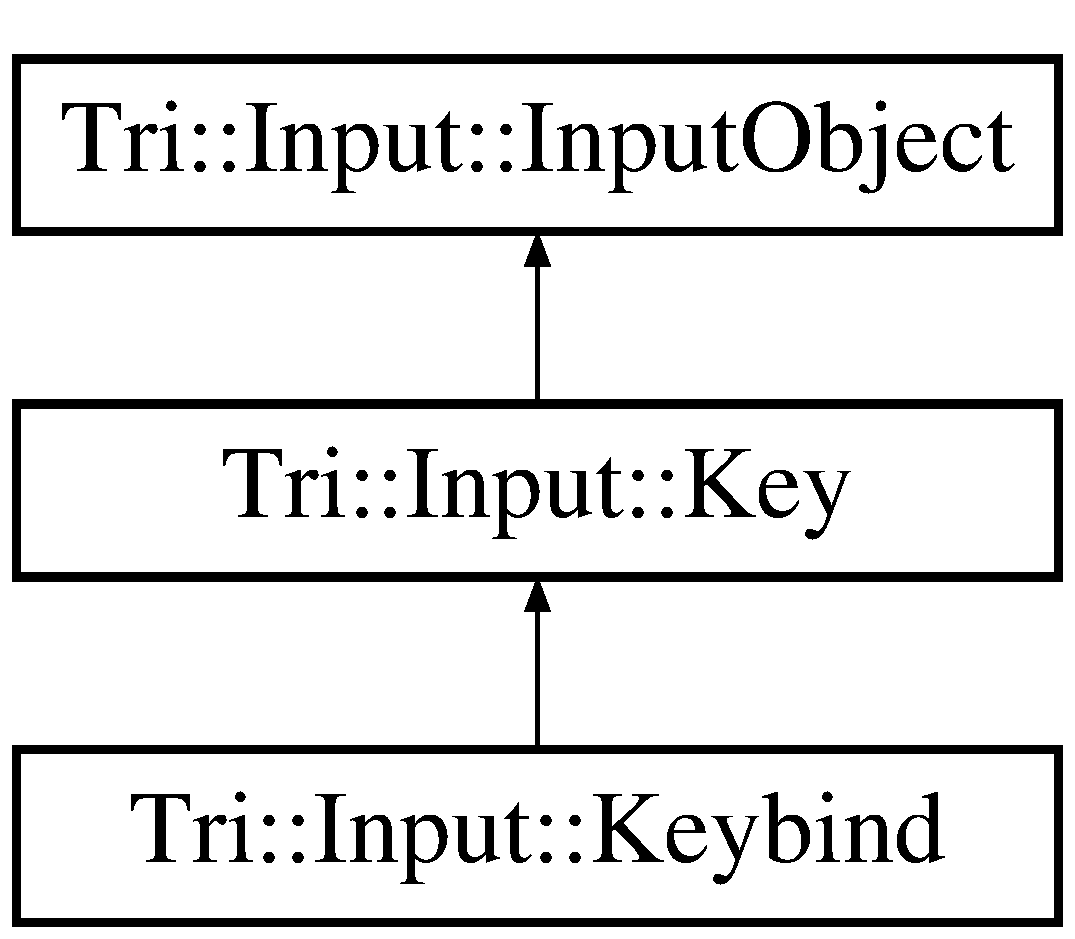
\includegraphics[height=3.000000cm]{class_tri_1_1_input_1_1_keybind}
\end{center}
\end{figure}
\subsection*{Public Types}
\begin{DoxyCompactItemize}
\item 
typedef void($\ast$ \hyperlink{class_tri_1_1_input_1_1_keybind_ad673cad554dbcc91f9158d0e28ddde35}{keycallfun}) (int, \hyperlink{namespace_tri_1_1_input_1_1_system_a79600e9f4ed835251eed1706ce96bed0}{System\+::\+Action}, int)
\begin{DoxyCompactList}\small\item\em The function signature for key callbacks. \end{DoxyCompactList}\end{DoxyCompactItemize}
\subsection*{Public Member Functions}
\begin{DoxyCompactItemize}
\item 
\hyperlink{class_tri_1_1_input_1_1_keybind_a24061b2a16170f851af53c4895b00c21}{Key\+Bind} (\hyperlink{struct_tri_1_1_input_1_1_key_a0b1f54fb1b7be8fe2e920ca8552f86dc}{Key\+Index} index)
\item 
void \hyperlink{class_tri_1_1_input_1_1_keybind_a4d71f6463f2e057e024fc6e4018b2207}{Set\+Key} (\hyperlink{struct_tri_1_1_input_1_1_key_a0b1f54fb1b7be8fe2e920ca8552f86dc}{Key\+Index} index)
\item 
void \hyperlink{class_tri_1_1_input_1_1_keybind_abdb6f9de4e66aed3c24f90c62aed1043}{Set\+Key\+Callback} (\hyperlink{class_tri_1_1_input_1_1_keybind_ad673cad554dbcc91f9158d0e28ddde35}{keycallfun} callback)
\end{DoxyCompactItemize}
\subsection*{Additional Inherited Members}


\subsection{Detailed Description}


Definition at line 64 of file key.\+h.



\subsection{Member Typedef Documentation}
\hypertarget{class_tri_1_1_input_1_1_keybind_ad673cad554dbcc91f9158d0e28ddde35}{}\index{Tri\+::\+Input\+::\+Keybind@{Tri\+::\+Input\+::\+Keybind}!keycallfun@{keycallfun}}
\index{keycallfun@{keycallfun}!Tri\+::\+Input\+::\+Keybind@{Tri\+::\+Input\+::\+Keybind}}
\subsubsection[{keycallfun}]{\setlength{\rightskip}{0pt plus 5cm}typedef void($\ast$  Tri\+::\+Input\+::\+Keybind\+::keycallfun) (int, {\bf System\+::\+Action}, int)}\label{class_tri_1_1_input_1_1_keybind_ad673cad554dbcc91f9158d0e28ddde35}


The function signature for key callbacks. 

The function signature for key callbacks for use with keybinds


\begin{DoxyParams}[1]{Parameters}
\mbox{\tt in}  & {\em scancode} & The scancode that is currently representing the key \\
\hline
\mbox{\tt in}  & {\em action} & The action the key is currently expressing \\
\hline
\mbox{\tt in}  & {\em mods} & The current bit field modifier describing what modifier keys were held \\
\hline
\end{DoxyParams}


Definition at line 75 of file key.\+h.



\subsection{Member Function Documentation}
\hypertarget{class_tri_1_1_input_1_1_keybind_a24061b2a16170f851af53c4895b00c21}{}\index{Tri\+::\+Input\+::\+Keybind@{Tri\+::\+Input\+::\+Keybind}!Key\+Bind@{Key\+Bind}}
\index{Key\+Bind@{Key\+Bind}!Tri\+::\+Input\+::\+Keybind@{Tri\+::\+Input\+::\+Keybind}}
\subsubsection[{Key\+Bind}]{\setlength{\rightskip}{0pt plus 5cm}Tri\+::\+Input\+::\+Keybind\+::\+Key\+Bind (
\begin{DoxyParamCaption}
\item[{{\bf Key\+Index}}]{index}
\end{DoxyParamCaption}
)\hspace{0.3cm}{\ttfamily [inline]}}\label{class_tri_1_1_input_1_1_keybind_a24061b2a16170f851af53c4895b00c21}


Definition at line 77 of file key.\+h.

\hypertarget{class_tri_1_1_input_1_1_keybind_a4d71f6463f2e057e024fc6e4018b2207}{}\index{Tri\+::\+Input\+::\+Keybind@{Tri\+::\+Input\+::\+Keybind}!Set\+Key@{Set\+Key}}
\index{Set\+Key@{Set\+Key}!Tri\+::\+Input\+::\+Keybind@{Tri\+::\+Input\+::\+Keybind}}
\subsubsection[{Set\+Key}]{\setlength{\rightskip}{0pt plus 5cm}void Tri\+::\+Input\+::\+Keybind\+::\+Set\+Key (
\begin{DoxyParamCaption}
\item[{{\bf Key\+Index}}]{index}
\end{DoxyParamCaption}
)}\label{class_tri_1_1_input_1_1_keybind_a4d71f6463f2e057e024fc6e4018b2207}
\hypertarget{class_tri_1_1_input_1_1_keybind_abdb6f9de4e66aed3c24f90c62aed1043}{}\index{Tri\+::\+Input\+::\+Keybind@{Tri\+::\+Input\+::\+Keybind}!Set\+Key\+Callback@{Set\+Key\+Callback}}
\index{Set\+Key\+Callback@{Set\+Key\+Callback}!Tri\+::\+Input\+::\+Keybind@{Tri\+::\+Input\+::\+Keybind}}
\subsubsection[{Set\+Key\+Callback}]{\setlength{\rightskip}{0pt plus 5cm}void Tri\+::\+Input\+::\+Keybind\+::\+Set\+Key\+Callback (
\begin{DoxyParamCaption}
\item[{{\bf keycallfun}}]{callback}
\end{DoxyParamCaption}
)}\label{class_tri_1_1_input_1_1_keybind_abdb6f9de4e66aed3c24f90c62aed1043}


The documentation for this class was generated from the following file\+:\begin{DoxyCompactItemize}
\item 
input/\hyperlink{key_8h}{key.\+h}\end{DoxyCompactItemize}

\hypertarget{class_triton_1_1_util_1_1_language}{}\section{Triton\+:\+:Util\+:\+:Language Class Reference}
\label{class_triton_1_1_util_1_1_language}\index{Triton\+::\+Util\+::\+Language@{Triton\+::\+Util\+::\+Language}}


The language object.  




{\ttfamily \#include $<$local.\+h$>$}

\subsection*{Public Member Functions}
\begin{DoxyCompactItemize}
\item 
\hyperlink{namespace_triton_1_1_util_ab36ffddebe19fdd103ec60af3841d9e2}{String} \hyperlink{class_triton_1_1_util_1_1_language_a16fd4d6c079f1a6d310dafe3c0587520}{Get\+Name} ()
\item 
\hyperlink{namespace_triton_1_1_util_ab36ffddebe19fdd103ec60af3841d9e2}{String} \hyperlink{class_triton_1_1_util_1_1_language_a9a2b45374aa49fa1dc9910afd92288c6}{Get\+Local} (\hyperlink{namespace_triton_1_1_util_ab36ffddebe19fdd103ec60af3841d9e2}{String} unlocalize\+Name)
\end{DoxyCompactItemize}
\subsection*{Friends}
\begin{DoxyCompactItemize}
\item 
class \hyperlink{class_triton_1_1_util_1_1_language_af7a1efe82e3beafa2fa9fc62c5ce5837}{Local\+Manager}
\end{DoxyCompactItemize}


\subsection{Detailed Description}
The language object. 

Definition at line 33 of file local.\+h.



\subsection{Member Function Documentation}
\hypertarget{class_triton_1_1_util_1_1_language_a9a2b45374aa49fa1dc9910afd92288c6}{}\index{Triton\+::\+Util\+::\+Language@{Triton\+::\+Util\+::\+Language}!Get\+Local@{Get\+Local}}
\index{Get\+Local@{Get\+Local}!Triton\+::\+Util\+::\+Language@{Triton\+::\+Util\+::\+Language}}
\subsubsection[{Get\+Local}]{\setlength{\rightskip}{0pt plus 5cm}{\bf String} Triton\+::\+Util\+::\+Language\+::\+Get\+Local (
\begin{DoxyParamCaption}
\item[{{\bf String}}]{unlocalize\+Name}
\end{DoxyParamCaption}
)}\label{class_triton_1_1_util_1_1_language_a9a2b45374aa49fa1dc9910afd92288c6}
\hypertarget{class_triton_1_1_util_1_1_language_a16fd4d6c079f1a6d310dafe3c0587520}{}\index{Triton\+::\+Util\+::\+Language@{Triton\+::\+Util\+::\+Language}!Get\+Name@{Get\+Name}}
\index{Get\+Name@{Get\+Name}!Triton\+::\+Util\+::\+Language@{Triton\+::\+Util\+::\+Language}}
\subsubsection[{Get\+Name}]{\setlength{\rightskip}{0pt plus 5cm}{\bf String} Triton\+::\+Util\+::\+Language\+::\+Get\+Name (
\begin{DoxyParamCaption}
{}
\end{DoxyParamCaption}
)}\label{class_triton_1_1_util_1_1_language_a16fd4d6c079f1a6d310dafe3c0587520}


\subsection{Friends And Related Function Documentation}
\hypertarget{class_triton_1_1_util_1_1_language_af7a1efe82e3beafa2fa9fc62c5ce5837}{}\index{Triton\+::\+Util\+::\+Language@{Triton\+::\+Util\+::\+Language}!Local\+Manager@{Local\+Manager}}
\index{Local\+Manager@{Local\+Manager}!Triton\+::\+Util\+::\+Language@{Triton\+::\+Util\+::\+Language}}
\subsubsection[{Local\+Manager}]{\setlength{\rightskip}{0pt plus 5cm}friend class {\bf Local\+Manager}\hspace{0.3cm}{\ttfamily [friend]}}\label{class_triton_1_1_util_1_1_language_af7a1efe82e3beafa2fa9fc62c5ce5837}


Definition at line 35 of file local.\+h.



The documentation for this class was generated from the following file\+:\begin{DoxyCompactItemize}
\item 
util/\hyperlink{local_8h}{local.\+h}\end{DoxyCompactItemize}

\hypertarget{class_triton_1_1_util_1_1_local_manager}{}\section{Triton\+:\+:Util\+:\+:Local\+Manager Class Reference}
\label{class_triton_1_1_util_1_1_local_manager}\index{Triton\+::\+Util\+::\+Local\+Manager@{Triton\+::\+Util\+::\+Local\+Manager}}


The manager for localization.  




{\ttfamily \#include $<$local.\+h$>$}

\subsection*{Public Member Functions}
\begin{DoxyCompactItemize}
\item 
void \hyperlink{class_triton_1_1_util_1_1_local_manager_a962122f655decc34b068b56118bc5b34}{Set\+Directory} (\hyperlink{namespace_triton_1_1_util_ab36ffddebe19fdd103ec60af3841d9e2}{String} directory)
\item 
\hyperlink{class_triton_1_1_util_1_1_language}{Language} \hyperlink{class_triton_1_1_util_1_1_local_manager_ae32d85010550cd6a5c76b5ae90263acf}{Get\+Language} (\hyperlink{namespace_triton_1_1_util_ab36ffddebe19fdd103ec60af3841d9e2}{String} name=\char`\"{}\char`\"{})
\end{DoxyCompactItemize}


\subsection{Detailed Description}
The manager for localization. 

Definition at line 18 of file local.\+h.



\subsection{Member Function Documentation}
\hypertarget{class_triton_1_1_util_1_1_local_manager_ae32d85010550cd6a5c76b5ae90263acf}{}\index{Triton\+::\+Util\+::\+Local\+Manager@{Triton\+::\+Util\+::\+Local\+Manager}!Get\+Language@{Get\+Language}}
\index{Get\+Language@{Get\+Language}!Triton\+::\+Util\+::\+Local\+Manager@{Triton\+::\+Util\+::\+Local\+Manager}}
\subsubsection[{Get\+Language}]{\setlength{\rightskip}{0pt plus 5cm}{\bf Language} Triton\+::\+Util\+::\+Local\+Manager\+::\+Get\+Language (
\begin{DoxyParamCaption}
\item[{{\bf String}}]{name = {\ttfamily \char`\"{}\char`\"{}}}
\end{DoxyParamCaption}
)}\label{class_triton_1_1_util_1_1_local_manager_ae32d85010550cd6a5c76b5ae90263acf}
\hypertarget{class_triton_1_1_util_1_1_local_manager_a962122f655decc34b068b56118bc5b34}{}\index{Triton\+::\+Util\+::\+Local\+Manager@{Triton\+::\+Util\+::\+Local\+Manager}!Set\+Directory@{Set\+Directory}}
\index{Set\+Directory@{Set\+Directory}!Triton\+::\+Util\+::\+Local\+Manager@{Triton\+::\+Util\+::\+Local\+Manager}}
\subsubsection[{Set\+Directory}]{\setlength{\rightskip}{0pt plus 5cm}void Triton\+::\+Util\+::\+Local\+Manager\+::\+Set\+Directory (
\begin{DoxyParamCaption}
\item[{{\bf String}}]{directory}
\end{DoxyParamCaption}
)}\label{class_triton_1_1_util_1_1_local_manager_a962122f655decc34b068b56118bc5b34}


The documentation for this class was generated from the following file\+:\begin{DoxyCompactItemize}
\item 
util/\hyperlink{local_8h}{local.\+h}\end{DoxyCompactItemize}

\hypertarget{class_tri_1_1_graphic_1_1_model}{}\section{Tri\+:\+:Graphic\+:\+:Model Class Reference}
\label{class_tri_1_1_graphic_1_1_model}\index{Tri\+::\+Graphic\+::\+Model@{Tri\+::\+Graphic\+::\+Model}}


{\ttfamily \#include $<$resource.\+h$>$}

\subsection*{Public Member Functions}
\begin{DoxyCompactItemize}
\item 
\hyperlink{class_tri_1_1_graphic_1_1_model_a57f8abc051d104b925e6a2cbb253b56c}{Model} (Util\+::\+D\+List$<$ Util\+::\+Vec3 $>$ vertices, Util\+::\+D\+List$<$ Util\+::\+Vec2 $>$ uvs, Util\+::\+D\+List$<$ Util\+::\+Vec3 $>$ normals)
\item 
Util\+::\+Vec3 \hyperlink{class_tri_1_1_graphic_1_1_model_af64f04fc0559ceb51061f8dfed0eb4e6}{Get\+Vertex} (int index)
\item 
Util\+::\+Vec2 \hyperlink{class_tri_1_1_graphic_1_1_model_a64da67596d9650b41ce0dd60f90eb7bb}{Get\+U\+V} (int index)
\item 
Util\+::\+Vec3 \hyperlink{class_tri_1_1_graphic_1_1_model_a086a31e07b32371a5d7d6c4629853cb9}{Get\+Normal} (int index)
\item 
void \hyperlink{class_tri_1_1_graphic_1_1_model_aa190ca9e2258a28ea12a36d7fb25b0de}{Render} (\hyperlink{class_tri_1_1_graphic_1_1_image}{Image} image)
\end{DoxyCompactItemize}
\subsection*{Static Public Member Functions}
\begin{DoxyCompactItemize}
\item 
static \hyperlink{class_tri_1_1_graphic_1_1_model}{Model} \hyperlink{class_tri_1_1_graphic_1_1_model_a779169e267e557ef11f86d561eecd8b2}{Get\+Obj} (Util\+::\+String filepath, bool invert\+Uv=false)
\end{DoxyCompactItemize}


\subsection{Detailed Description}


Definition at line 28 of file resource.\+h.



\subsection{Constructor \& Destructor Documentation}
\hypertarget{class_tri_1_1_graphic_1_1_model_a57f8abc051d104b925e6a2cbb253b56c}{}\index{Tri\+::\+Graphic\+::\+Model@{Tri\+::\+Graphic\+::\+Model}!Model@{Model}}
\index{Model@{Model}!Tri\+::\+Graphic\+::\+Model@{Tri\+::\+Graphic\+::\+Model}}
\subsubsection[{Model}]{\setlength{\rightskip}{0pt plus 5cm}Tri\+::\+Graphic\+::\+Model\+::\+Model (
\begin{DoxyParamCaption}
\item[{Util\+::\+D\+List$<$ Util\+::\+Vec3 $>$}]{vertices, }
\item[{Util\+::\+D\+List$<$ Util\+::\+Vec2 $>$}]{uvs, }
\item[{Util\+::\+D\+List$<$ Util\+::\+Vec3 $>$}]{normals}
\end{DoxyParamCaption}
)}\label{class_tri_1_1_graphic_1_1_model_a57f8abc051d104b925e6a2cbb253b56c}


\subsection{Member Function Documentation}
\hypertarget{class_tri_1_1_graphic_1_1_model_a086a31e07b32371a5d7d6c4629853cb9}{}\index{Tri\+::\+Graphic\+::\+Model@{Tri\+::\+Graphic\+::\+Model}!Get\+Normal@{Get\+Normal}}
\index{Get\+Normal@{Get\+Normal}!Tri\+::\+Graphic\+::\+Model@{Tri\+::\+Graphic\+::\+Model}}
\subsubsection[{Get\+Normal}]{\setlength{\rightskip}{0pt plus 5cm}Util\+::\+Vec3 Tri\+::\+Graphic\+::\+Model\+::\+Get\+Normal (
\begin{DoxyParamCaption}
\item[{int}]{index}
\end{DoxyParamCaption}
)}\label{class_tri_1_1_graphic_1_1_model_a086a31e07b32371a5d7d6c4629853cb9}
\hypertarget{class_tri_1_1_graphic_1_1_model_a779169e267e557ef11f86d561eecd8b2}{}\index{Tri\+::\+Graphic\+::\+Model@{Tri\+::\+Graphic\+::\+Model}!Get\+Obj@{Get\+Obj}}
\index{Get\+Obj@{Get\+Obj}!Tri\+::\+Graphic\+::\+Model@{Tri\+::\+Graphic\+::\+Model}}
\subsubsection[{Get\+Obj}]{\setlength{\rightskip}{0pt plus 5cm}static {\bf Model} Tri\+::\+Graphic\+::\+Model\+::\+Get\+Obj (
\begin{DoxyParamCaption}
\item[{Util\+::\+String}]{filepath, }
\item[{bool}]{invert\+Uv = {\ttfamily false}}
\end{DoxyParamCaption}
)\hspace{0.3cm}{\ttfamily [static]}}\label{class_tri_1_1_graphic_1_1_model_a779169e267e557ef11f86d561eecd8b2}
\hypertarget{class_tri_1_1_graphic_1_1_model_a64da67596d9650b41ce0dd60f90eb7bb}{}\index{Tri\+::\+Graphic\+::\+Model@{Tri\+::\+Graphic\+::\+Model}!Get\+U\+V@{Get\+U\+V}}
\index{Get\+U\+V@{Get\+U\+V}!Tri\+::\+Graphic\+::\+Model@{Tri\+::\+Graphic\+::\+Model}}
\subsubsection[{Get\+U\+V}]{\setlength{\rightskip}{0pt plus 5cm}Util\+::\+Vec2 Tri\+::\+Graphic\+::\+Model\+::\+Get\+U\+V (
\begin{DoxyParamCaption}
\item[{int}]{index}
\end{DoxyParamCaption}
)}\label{class_tri_1_1_graphic_1_1_model_a64da67596d9650b41ce0dd60f90eb7bb}
\hypertarget{class_tri_1_1_graphic_1_1_model_af64f04fc0559ceb51061f8dfed0eb4e6}{}\index{Tri\+::\+Graphic\+::\+Model@{Tri\+::\+Graphic\+::\+Model}!Get\+Vertex@{Get\+Vertex}}
\index{Get\+Vertex@{Get\+Vertex}!Tri\+::\+Graphic\+::\+Model@{Tri\+::\+Graphic\+::\+Model}}
\subsubsection[{Get\+Vertex}]{\setlength{\rightskip}{0pt plus 5cm}Util\+::\+Vec3 Tri\+::\+Graphic\+::\+Model\+::\+Get\+Vertex (
\begin{DoxyParamCaption}
\item[{int}]{index}
\end{DoxyParamCaption}
)}\label{class_tri_1_1_graphic_1_1_model_af64f04fc0559ceb51061f8dfed0eb4e6}
\hypertarget{class_tri_1_1_graphic_1_1_model_aa190ca9e2258a28ea12a36d7fb25b0de}{}\index{Tri\+::\+Graphic\+::\+Model@{Tri\+::\+Graphic\+::\+Model}!Render@{Render}}
\index{Render@{Render}!Tri\+::\+Graphic\+::\+Model@{Tri\+::\+Graphic\+::\+Model}}
\subsubsection[{Render}]{\setlength{\rightskip}{0pt plus 5cm}void Tri\+::\+Graphic\+::\+Model\+::\+Render (
\begin{DoxyParamCaption}
\item[{{\bf Image}}]{image}
\end{DoxyParamCaption}
)}\label{class_tri_1_1_graphic_1_1_model_aa190ca9e2258a28ea12a36d7fb25b0de}


The documentation for this class was generated from the following file\+:\begin{DoxyCompactItemize}
\item 
graphic/\hyperlink{resource_8h}{resource.\+h}\end{DoxyCompactItemize}

\hypertarget{class_tri_1_1_input_1_1_mouse}{}\section{Tri\+:\+:Input\+:\+:Mouse Class Reference}
\label{class_tri_1_1_input_1_1_mouse}\index{Tri\+::\+Input\+::\+Mouse@{Tri\+::\+Input\+::\+Mouse}}


{\ttfamily \#include $<$mouse.\+h$>$}

Inheritance diagram for Tri\+:\+:Input\+:\+:Mouse\+:\begin{figure}[H]
\begin{center}
\leavevmode
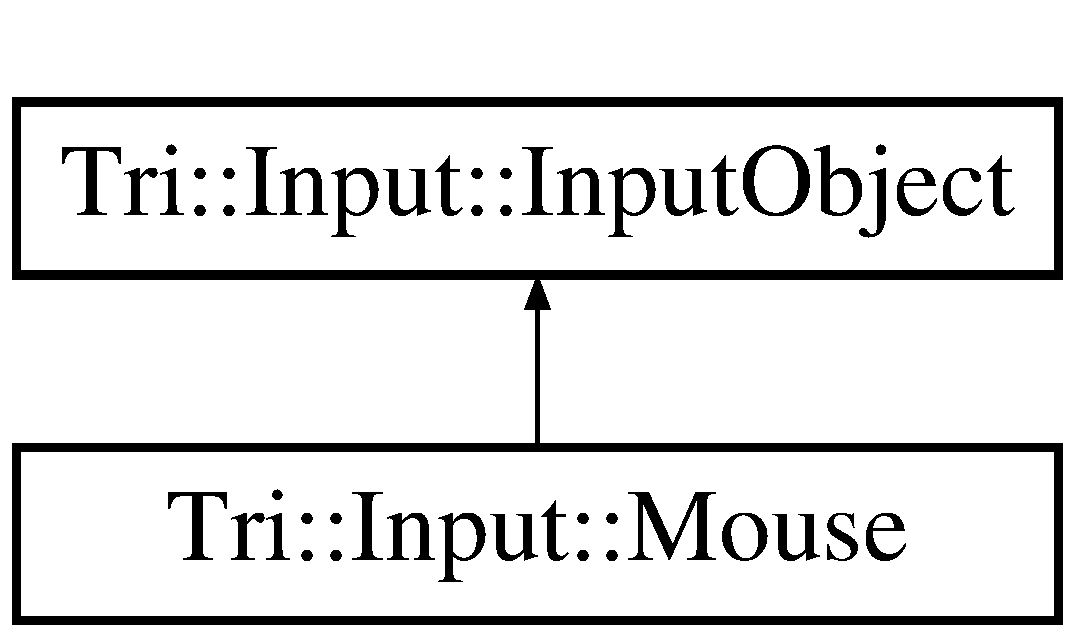
\includegraphics[height=2.000000cm]{class_tri_1_1_input_1_1_mouse}
\end{center}
\end{figure}
\subsection*{Public Types}
\begin{DoxyCompactItemize}
\item 
enum \hyperlink{class_tri_1_1_input_1_1_mouse_a926c664faabb33e4fab8154520289d2d}{Mouse\+Button} \{ \\*
\hyperlink{class_tri_1_1_input_1_1_mouse_a926c664faabb33e4fab8154520289d2da6b36fce26c3e0de5d0c85a958524bef1}{B\+U\+T\+T\+O\+N\+\_\+1}, 
\hyperlink{class_tri_1_1_input_1_1_mouse_a926c664faabb33e4fab8154520289d2da92ad49442fe1692838b77e30bcaa8ed0}{B\+U\+T\+T\+O\+N\+\_\+2}, 
\hyperlink{class_tri_1_1_input_1_1_mouse_a926c664faabb33e4fab8154520289d2dad58f3ede46ba5bdada2c9dba13b42b1e}{B\+U\+T\+T\+O\+N\+\_\+3}, 
\hyperlink{class_tri_1_1_input_1_1_mouse_a926c664faabb33e4fab8154520289d2da9dcd0194cddaf80e354195445de0db6f}{B\+U\+T\+T\+O\+N\+\_\+4}, 
\\*
\hyperlink{class_tri_1_1_input_1_1_mouse_a926c664faabb33e4fab8154520289d2dad8aac1f1a0b61c908602fec899113063}{B\+U\+T\+T\+O\+N\+\_\+5}, 
\hyperlink{class_tri_1_1_input_1_1_mouse_a926c664faabb33e4fab8154520289d2da8542df531f31fe69ee8a4aff2ba1f107}{B\+U\+T\+T\+O\+N\+\_\+6}, 
\hyperlink{class_tri_1_1_input_1_1_mouse_a926c664faabb33e4fab8154520289d2da5d9fce5e7926344120fef52dd8308b83}{B\+U\+T\+T\+O\+N\+\_\+7}, 
\hyperlink{class_tri_1_1_input_1_1_mouse_a926c664faabb33e4fab8154520289d2dadedec5dea3469ba5108e9c55b4cc7ef0}{B\+U\+T\+T\+O\+N\+\_\+8}, 
\\*
\hyperlink{class_tri_1_1_input_1_1_mouse_a926c664faabb33e4fab8154520289d2da46a51cfaf13bbe1808d3fb11ba4388dc}{L\+A\+S\+T\+\_\+\+B\+U\+T\+T\+O\+N} = B\+U\+T\+T\+O\+N\+\_\+8, 
\hyperlink{class_tri_1_1_input_1_1_mouse_a926c664faabb33e4fab8154520289d2dabe1025e97865151850300ae0ff72fc99}{L\+E\+F\+T\+\_\+\+B\+U\+T\+T\+O\+N} = B\+U\+T\+T\+O\+N\+\_\+1, 
\hyperlink{class_tri_1_1_input_1_1_mouse_a926c664faabb33e4fab8154520289d2dac76191c266b674f8fe6b5c9af8eb9c6a}{R\+I\+G\+H\+T\+\_\+\+B\+U\+T\+T\+O\+N} = B\+U\+T\+T\+O\+N\+\_\+2, 
\hyperlink{class_tri_1_1_input_1_1_mouse_a926c664faabb33e4fab8154520289d2dab42854e62393785b1cb2f0be34741815}{M\+I\+D\+D\+L\+E\+\_\+\+B\+U\+T\+T\+O\+N} = B\+U\+T\+T\+O\+N\+\_\+3
 \}
\item 
typedef void($\ast$ \hyperlink{class_tri_1_1_input_1_1_mouse_a41472f0b88d5fd25c219575da51e8e0b}{mousecallfun}) (\hyperlink{class_tri_1_1_input_1_1_mouse_a926c664faabb33e4fab8154520289d2d}{Mouse\+Button}, \hyperlink{namespace_tri_1_1_input_1_1_system_a79600e9f4ed835251eed1706ce96bed0}{System\+::\+Action}, int)
\begin{DoxyCompactList}\small\item\em The function signature for mouse callbacks. \end{DoxyCompactList}\end{DoxyCompactItemize}
\subsection*{Public Member Functions}
\begin{DoxyCompactItemize}
\item 
\hyperlink{namespace_tri_1_1_input_1_1_system_a79600e9f4ed835251eed1706ce96bed0}{System\+::\+Action} \hyperlink{class_tri_1_1_input_1_1_mouse_a7c94e7c24b8b7792021d58cceb78f89b}{Get\+Button\+Action} (\hyperlink{class_tri_1_1_input_1_1_mouse_a926c664faabb33e4fab8154520289d2d}{Mouse\+Button} button)
\item 
void \hyperlink{class_tri_1_1_input_1_1_mouse_a193562bc5a6f21f420c0aa32b64317a1}{Set\+Mouse\+Callback} (\hyperlink{class_tri_1_1_input_1_1_mouse_a41472f0b88d5fd25c219575da51e8e0b}{mousecallfun} callback)
\end{DoxyCompactItemize}
\subsection*{Protected Member Functions}
\begin{DoxyCompactItemize}
\item 
\hyperlink{class_tri_1_1_input_1_1_mouse_af4442e246b375684a579eddf12c85c7f}{Mouse} (\hyperlink{namespace_tri_1_1_input_ac94df02dceb9dbc5ca1512e9ded38154}{Input\+I\+D} id)
\end{DoxyCompactItemize}


\subsection{Detailed Description}


Definition at line 10 of file mouse.\+h.



\subsection{Member Typedef Documentation}
\hypertarget{class_tri_1_1_input_1_1_mouse_a41472f0b88d5fd25c219575da51e8e0b}{}\index{Tri\+::\+Input\+::\+Mouse@{Tri\+::\+Input\+::\+Mouse}!mousecallfun@{mousecallfun}}
\index{mousecallfun@{mousecallfun}!Tri\+::\+Input\+::\+Mouse@{Tri\+::\+Input\+::\+Mouse}}
\subsubsection[{mousecallfun}]{\setlength{\rightskip}{0pt plus 5cm}typedef void($\ast$  Tri\+::\+Input\+::\+Mouse\+::mousecallfun) ({\bf Mouse\+Button}, {\bf System\+::\+Action}, int)}\label{class_tri_1_1_input_1_1_mouse_a41472f0b88d5fd25c219575da51e8e0b}


The function signature for mouse callbacks. 

The function signature for mouse callbacks


\begin{DoxyParams}[1]{Parameters}
\mbox{\tt in}  & {\em mouse\+Button} & The current checked \hyperlink{class_tri_1_1_input_1_1_mouse_a926c664faabb33e4fab8154520289d2d}{Mouse Button} \\
\hline
\mbox{\tt in}  & {\em action} & The action the button is currently expressing \\
\hline
\mbox{\tt in}  & {\em mods} & The current bit field modifier describing what modifier keys were held \\
\hline
\end{DoxyParams}


Definition at line 37 of file mouse.\+h.



\subsection{Member Enumeration Documentation}
\hypertarget{class_tri_1_1_input_1_1_mouse_a926c664faabb33e4fab8154520289d2d}{}\index{Tri\+::\+Input\+::\+Mouse@{Tri\+::\+Input\+::\+Mouse}!Mouse\+Button@{Mouse\+Button}}
\index{Mouse\+Button@{Mouse\+Button}!Tri\+::\+Input\+::\+Mouse@{Tri\+::\+Input\+::\+Mouse}}
\subsubsection[{Mouse\+Button}]{\setlength{\rightskip}{0pt plus 5cm}enum {\bf Tri\+::\+Input\+::\+Mouse\+::\+Mouse\+Button}}\label{class_tri_1_1_input_1_1_mouse_a926c664faabb33e4fab8154520289d2d}
\begin{Desc}
\item[Enumerator]\par
\begin{description}
\index{B\+U\+T\+T\+O\+N\+\_\+1@{B\+U\+T\+T\+O\+N\+\_\+1}!Tri\+::\+Input\+::\+Mouse@{Tri\+::\+Input\+::\+Mouse}}\index{Tri\+::\+Input\+::\+Mouse@{Tri\+::\+Input\+::\+Mouse}!B\+U\+T\+T\+O\+N\+\_\+1@{B\+U\+T\+T\+O\+N\+\_\+1}}\item[{\em 
\hypertarget{class_tri_1_1_input_1_1_mouse_a926c664faabb33e4fab8154520289d2da6b36fce26c3e0de5d0c85a958524bef1}{}B\+U\+T\+T\+O\+N\+\_\+1\label{class_tri_1_1_input_1_1_mouse_a926c664faabb33e4fab8154520289d2da6b36fce26c3e0de5d0c85a958524bef1}
}]\index{B\+U\+T\+T\+O\+N\+\_\+2@{B\+U\+T\+T\+O\+N\+\_\+2}!Tri\+::\+Input\+::\+Mouse@{Tri\+::\+Input\+::\+Mouse}}\index{Tri\+::\+Input\+::\+Mouse@{Tri\+::\+Input\+::\+Mouse}!B\+U\+T\+T\+O\+N\+\_\+2@{B\+U\+T\+T\+O\+N\+\_\+2}}\item[{\em 
\hypertarget{class_tri_1_1_input_1_1_mouse_a926c664faabb33e4fab8154520289d2da92ad49442fe1692838b77e30bcaa8ed0}{}B\+U\+T\+T\+O\+N\+\_\+2\label{class_tri_1_1_input_1_1_mouse_a926c664faabb33e4fab8154520289d2da92ad49442fe1692838b77e30bcaa8ed0}
}]\index{B\+U\+T\+T\+O\+N\+\_\+3@{B\+U\+T\+T\+O\+N\+\_\+3}!Tri\+::\+Input\+::\+Mouse@{Tri\+::\+Input\+::\+Mouse}}\index{Tri\+::\+Input\+::\+Mouse@{Tri\+::\+Input\+::\+Mouse}!B\+U\+T\+T\+O\+N\+\_\+3@{B\+U\+T\+T\+O\+N\+\_\+3}}\item[{\em 
\hypertarget{class_tri_1_1_input_1_1_mouse_a926c664faabb33e4fab8154520289d2dad58f3ede46ba5bdada2c9dba13b42b1e}{}B\+U\+T\+T\+O\+N\+\_\+3\label{class_tri_1_1_input_1_1_mouse_a926c664faabb33e4fab8154520289d2dad58f3ede46ba5bdada2c9dba13b42b1e}
}]\index{B\+U\+T\+T\+O\+N\+\_\+4@{B\+U\+T\+T\+O\+N\+\_\+4}!Tri\+::\+Input\+::\+Mouse@{Tri\+::\+Input\+::\+Mouse}}\index{Tri\+::\+Input\+::\+Mouse@{Tri\+::\+Input\+::\+Mouse}!B\+U\+T\+T\+O\+N\+\_\+4@{B\+U\+T\+T\+O\+N\+\_\+4}}\item[{\em 
\hypertarget{class_tri_1_1_input_1_1_mouse_a926c664faabb33e4fab8154520289d2da9dcd0194cddaf80e354195445de0db6f}{}B\+U\+T\+T\+O\+N\+\_\+4\label{class_tri_1_1_input_1_1_mouse_a926c664faabb33e4fab8154520289d2da9dcd0194cddaf80e354195445de0db6f}
}]\index{B\+U\+T\+T\+O\+N\+\_\+5@{B\+U\+T\+T\+O\+N\+\_\+5}!Tri\+::\+Input\+::\+Mouse@{Tri\+::\+Input\+::\+Mouse}}\index{Tri\+::\+Input\+::\+Mouse@{Tri\+::\+Input\+::\+Mouse}!B\+U\+T\+T\+O\+N\+\_\+5@{B\+U\+T\+T\+O\+N\+\_\+5}}\item[{\em 
\hypertarget{class_tri_1_1_input_1_1_mouse_a926c664faabb33e4fab8154520289d2dad8aac1f1a0b61c908602fec899113063}{}B\+U\+T\+T\+O\+N\+\_\+5\label{class_tri_1_1_input_1_1_mouse_a926c664faabb33e4fab8154520289d2dad8aac1f1a0b61c908602fec899113063}
}]\index{B\+U\+T\+T\+O\+N\+\_\+6@{B\+U\+T\+T\+O\+N\+\_\+6}!Tri\+::\+Input\+::\+Mouse@{Tri\+::\+Input\+::\+Mouse}}\index{Tri\+::\+Input\+::\+Mouse@{Tri\+::\+Input\+::\+Mouse}!B\+U\+T\+T\+O\+N\+\_\+6@{B\+U\+T\+T\+O\+N\+\_\+6}}\item[{\em 
\hypertarget{class_tri_1_1_input_1_1_mouse_a926c664faabb33e4fab8154520289d2da8542df531f31fe69ee8a4aff2ba1f107}{}B\+U\+T\+T\+O\+N\+\_\+6\label{class_tri_1_1_input_1_1_mouse_a926c664faabb33e4fab8154520289d2da8542df531f31fe69ee8a4aff2ba1f107}
}]\index{B\+U\+T\+T\+O\+N\+\_\+7@{B\+U\+T\+T\+O\+N\+\_\+7}!Tri\+::\+Input\+::\+Mouse@{Tri\+::\+Input\+::\+Mouse}}\index{Tri\+::\+Input\+::\+Mouse@{Tri\+::\+Input\+::\+Mouse}!B\+U\+T\+T\+O\+N\+\_\+7@{B\+U\+T\+T\+O\+N\+\_\+7}}\item[{\em 
\hypertarget{class_tri_1_1_input_1_1_mouse_a926c664faabb33e4fab8154520289d2da5d9fce5e7926344120fef52dd8308b83}{}B\+U\+T\+T\+O\+N\+\_\+7\label{class_tri_1_1_input_1_1_mouse_a926c664faabb33e4fab8154520289d2da5d9fce5e7926344120fef52dd8308b83}
}]\index{B\+U\+T\+T\+O\+N\+\_\+8@{B\+U\+T\+T\+O\+N\+\_\+8}!Tri\+::\+Input\+::\+Mouse@{Tri\+::\+Input\+::\+Mouse}}\index{Tri\+::\+Input\+::\+Mouse@{Tri\+::\+Input\+::\+Mouse}!B\+U\+T\+T\+O\+N\+\_\+8@{B\+U\+T\+T\+O\+N\+\_\+8}}\item[{\em 
\hypertarget{class_tri_1_1_input_1_1_mouse_a926c664faabb33e4fab8154520289d2dadedec5dea3469ba5108e9c55b4cc7ef0}{}B\+U\+T\+T\+O\+N\+\_\+8\label{class_tri_1_1_input_1_1_mouse_a926c664faabb33e4fab8154520289d2dadedec5dea3469ba5108e9c55b4cc7ef0}
}]\index{L\+A\+S\+T\+\_\+\+B\+U\+T\+T\+O\+N@{L\+A\+S\+T\+\_\+\+B\+U\+T\+T\+O\+N}!Tri\+::\+Input\+::\+Mouse@{Tri\+::\+Input\+::\+Mouse}}\index{Tri\+::\+Input\+::\+Mouse@{Tri\+::\+Input\+::\+Mouse}!L\+A\+S\+T\+\_\+\+B\+U\+T\+T\+O\+N@{L\+A\+S\+T\+\_\+\+B\+U\+T\+T\+O\+N}}\item[{\em 
\hypertarget{class_tri_1_1_input_1_1_mouse_a926c664faabb33e4fab8154520289d2da46a51cfaf13bbe1808d3fb11ba4388dc}{}L\+A\+S\+T\+\_\+\+B\+U\+T\+T\+O\+N\label{class_tri_1_1_input_1_1_mouse_a926c664faabb33e4fab8154520289d2da46a51cfaf13bbe1808d3fb11ba4388dc}
}]\index{L\+E\+F\+T\+\_\+\+B\+U\+T\+T\+O\+N@{L\+E\+F\+T\+\_\+\+B\+U\+T\+T\+O\+N}!Tri\+::\+Input\+::\+Mouse@{Tri\+::\+Input\+::\+Mouse}}\index{Tri\+::\+Input\+::\+Mouse@{Tri\+::\+Input\+::\+Mouse}!L\+E\+F\+T\+\_\+\+B\+U\+T\+T\+O\+N@{L\+E\+F\+T\+\_\+\+B\+U\+T\+T\+O\+N}}\item[{\em 
\hypertarget{class_tri_1_1_input_1_1_mouse_a926c664faabb33e4fab8154520289d2dabe1025e97865151850300ae0ff72fc99}{}L\+E\+F\+T\+\_\+\+B\+U\+T\+T\+O\+N\label{class_tri_1_1_input_1_1_mouse_a926c664faabb33e4fab8154520289d2dabe1025e97865151850300ae0ff72fc99}
}]\index{R\+I\+G\+H\+T\+\_\+\+B\+U\+T\+T\+O\+N@{R\+I\+G\+H\+T\+\_\+\+B\+U\+T\+T\+O\+N}!Tri\+::\+Input\+::\+Mouse@{Tri\+::\+Input\+::\+Mouse}}\index{Tri\+::\+Input\+::\+Mouse@{Tri\+::\+Input\+::\+Mouse}!R\+I\+G\+H\+T\+\_\+\+B\+U\+T\+T\+O\+N@{R\+I\+G\+H\+T\+\_\+\+B\+U\+T\+T\+O\+N}}\item[{\em 
\hypertarget{class_tri_1_1_input_1_1_mouse_a926c664faabb33e4fab8154520289d2dac76191c266b674f8fe6b5c9af8eb9c6a}{}R\+I\+G\+H\+T\+\_\+\+B\+U\+T\+T\+O\+N\label{class_tri_1_1_input_1_1_mouse_a926c664faabb33e4fab8154520289d2dac76191c266b674f8fe6b5c9af8eb9c6a}
}]\index{M\+I\+D\+D\+L\+E\+\_\+\+B\+U\+T\+T\+O\+N@{M\+I\+D\+D\+L\+E\+\_\+\+B\+U\+T\+T\+O\+N}!Tri\+::\+Input\+::\+Mouse@{Tri\+::\+Input\+::\+Mouse}}\index{Tri\+::\+Input\+::\+Mouse@{Tri\+::\+Input\+::\+Mouse}!M\+I\+D\+D\+L\+E\+\_\+\+B\+U\+T\+T\+O\+N@{M\+I\+D\+D\+L\+E\+\_\+\+B\+U\+T\+T\+O\+N}}\item[{\em 
\hypertarget{class_tri_1_1_input_1_1_mouse_a926c664faabb33e4fab8154520289d2dab42854e62393785b1cb2f0be34741815}{}M\+I\+D\+D\+L\+E\+\_\+\+B\+U\+T\+T\+O\+N\label{class_tri_1_1_input_1_1_mouse_a926c664faabb33e4fab8154520289d2dab42854e62393785b1cb2f0be34741815}
}]\end{description}
\end{Desc}


Definition at line 13 of file mouse.\+h.



\subsection{Constructor \& Destructor Documentation}
\hypertarget{class_tri_1_1_input_1_1_mouse_af4442e246b375684a579eddf12c85c7f}{}\index{Tri\+::\+Input\+::\+Mouse@{Tri\+::\+Input\+::\+Mouse}!Mouse@{Mouse}}
\index{Mouse@{Mouse}!Tri\+::\+Input\+::\+Mouse@{Tri\+::\+Input\+::\+Mouse}}
\subsubsection[{Mouse}]{\setlength{\rightskip}{0pt plus 5cm}Tri\+::\+Input\+::\+Mouse\+::\+Mouse (
\begin{DoxyParamCaption}
\item[{{\bf Input\+I\+D}}]{id}
\end{DoxyParamCaption}
)\hspace{0.3cm}{\ttfamily [protected]}}\label{class_tri_1_1_input_1_1_mouse_af4442e246b375684a579eddf12c85c7f}


\subsection{Member Function Documentation}
\hypertarget{class_tri_1_1_input_1_1_mouse_a7c94e7c24b8b7792021d58cceb78f89b}{}\index{Tri\+::\+Input\+::\+Mouse@{Tri\+::\+Input\+::\+Mouse}!Get\+Button\+Action@{Get\+Button\+Action}}
\index{Get\+Button\+Action@{Get\+Button\+Action}!Tri\+::\+Input\+::\+Mouse@{Tri\+::\+Input\+::\+Mouse}}
\subsubsection[{Get\+Button\+Action}]{\setlength{\rightskip}{0pt plus 5cm}{\bf System\+::\+Action} Tri\+::\+Input\+::\+Mouse\+::\+Get\+Button\+Action (
\begin{DoxyParamCaption}
\item[{{\bf Mouse\+Button}}]{button}
\end{DoxyParamCaption}
)}\label{class_tri_1_1_input_1_1_mouse_a7c94e7c24b8b7792021d58cceb78f89b}
\hypertarget{class_tri_1_1_input_1_1_mouse_a193562bc5a6f21f420c0aa32b64317a1}{}\index{Tri\+::\+Input\+::\+Mouse@{Tri\+::\+Input\+::\+Mouse}!Set\+Mouse\+Callback@{Set\+Mouse\+Callback}}
\index{Set\+Mouse\+Callback@{Set\+Mouse\+Callback}!Tri\+::\+Input\+::\+Mouse@{Tri\+::\+Input\+::\+Mouse}}
\subsubsection[{Set\+Mouse\+Callback}]{\setlength{\rightskip}{0pt plus 5cm}void Tri\+::\+Input\+::\+Mouse\+::\+Set\+Mouse\+Callback (
\begin{DoxyParamCaption}
\item[{{\bf mousecallfun}}]{callback}
\end{DoxyParamCaption}
)}\label{class_tri_1_1_input_1_1_mouse_a193562bc5a6f21f420c0aa32b64317a1}


The documentation for this class was generated from the following file\+:\begin{DoxyCompactItemize}
\item 
input/\hyperlink{mouse_8h}{mouse.\+h}\end{DoxyCompactItemize}

\hypertarget{struct_triton_1_1_util_1_1_radian}{}\section{Triton\+:\+:Util\+:\+:Radian Struct Reference}
\label{struct_triton_1_1_util_1_1_radian}\index{Triton\+::\+Util\+::\+Radian@{Triton\+::\+Util\+::\+Radian}}


A simplistic \hyperlink{struct_triton_1_1_util_1_1_radian}{Radian} object.  




{\ttfamily \#include $<$angle.\+h$>$}

Inheritance diagram for Triton\+:\+:Util\+:\+:Radian\+:\begin{figure}[H]
\begin{center}
\leavevmode
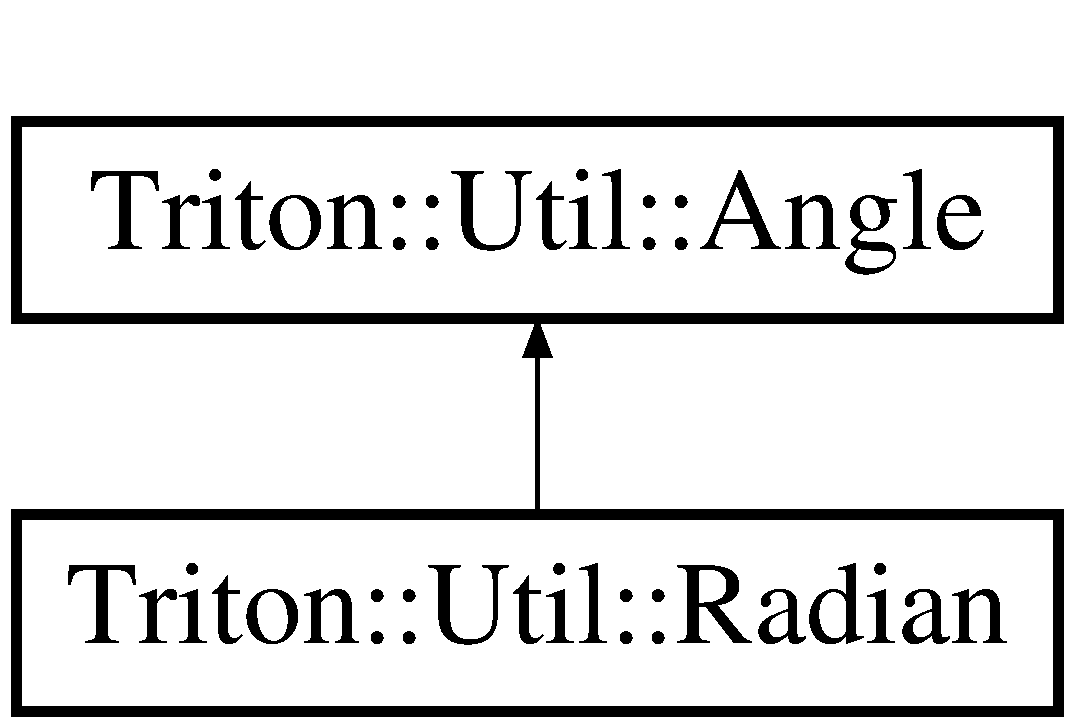
\includegraphics[height=2.000000cm]{struct_triton_1_1_util_1_1_radian}
\end{center}
\end{figure}
\subsection*{Public Member Functions}
\begin{DoxyCompactItemize}
\item 
\hyperlink{struct_triton_1_1_util_1_1_radian_a8a3742b1fea5004220873adc6d437d7c}{Radian} (float \hyperlink{struct_triton_1_1_util_1_1_angle_af7d7f20a28c150b09776a35bc1dae0c4}{ang})
\item 
\hyperlink{struct_triton_1_1_util_1_1_radian_a8f9ab085fc95a855c92cbafb25e6afd8}{Radian} (const \hyperlink{struct_triton_1_1_util_1_1_degree}{Degree} \&deg)
\item 
\hyperlink{struct_triton_1_1_util_1_1_degree}{Degree} \& \hyperlink{struct_triton_1_1_util_1_1_radian_aae924a8168ac832c6cccea1a37254f3b}{operator=} (const \hyperlink{struct_triton_1_1_util_1_1_radian}{Radian} \&rad)
\item 
\hyperlink{struct_triton_1_1_util_1_1_radian_a2ee78bac3381aa4c8bfd8eb92309a104}{operator Radian} ()
\item 
\hyperlink{struct_triton_1_1_util_1_1_degree}{Degree} \hyperlink{struct_triton_1_1_util_1_1_radian_a9c0762747497079361565baf13b098d4}{To\+Degree} ()
\item 
Rotation\+Type \hyperlink{struct_triton_1_1_util_1_1_radian_a75a4253af1ecb0bd75240fc604b8c61b}{Get\+Rotation\+Type} ()
\end{DoxyCompactItemize}
\subsection*{Additional Inherited Members}


\subsection{Detailed Description}
A simplistic \hyperlink{struct_triton_1_1_util_1_1_radian}{Radian} object. 

Based on \hyperlink{struct_triton_1_1_util_1_1_angle}{Angle} 

Definition at line 52 of file angle.\+h.



\subsection{Constructor \& Destructor Documentation}
\hypertarget{struct_triton_1_1_util_1_1_radian_a8a3742b1fea5004220873adc6d437d7c}{}\index{Triton\+::\+Util\+::\+Radian@{Triton\+::\+Util\+::\+Radian}!Radian@{Radian}}
\index{Radian@{Radian}!Triton\+::\+Util\+::\+Radian@{Triton\+::\+Util\+::\+Radian}}
\subsubsection[{Radian}]{\setlength{\rightskip}{0pt plus 5cm}Triton\+::\+Util\+::\+Radian\+::\+Radian (
\begin{DoxyParamCaption}
\item[{float}]{ang}
\end{DoxyParamCaption}
)\hspace{0.3cm}{\ttfamily [inline]}}\label{struct_triton_1_1_util_1_1_radian_a8a3742b1fea5004220873adc6d437d7c}


Definition at line 54 of file angle.\+h.

\hypertarget{struct_triton_1_1_util_1_1_radian_a8f9ab085fc95a855c92cbafb25e6afd8}{}\index{Triton\+::\+Util\+::\+Radian@{Triton\+::\+Util\+::\+Radian}!Radian@{Radian}}
\index{Radian@{Radian}!Triton\+::\+Util\+::\+Radian@{Triton\+::\+Util\+::\+Radian}}
\subsubsection[{Radian}]{\setlength{\rightskip}{0pt plus 5cm}Triton\+::\+Util\+::\+Radian\+::\+Radian (
\begin{DoxyParamCaption}
\item[{const {\bf Degree} \&}]{deg}
\end{DoxyParamCaption}
)}\label{struct_triton_1_1_util_1_1_radian_a8f9ab085fc95a855c92cbafb25e6afd8}


\subsection{Member Function Documentation}
\hypertarget{struct_triton_1_1_util_1_1_radian_a75a4253af1ecb0bd75240fc604b8c61b}{}\index{Triton\+::\+Util\+::\+Radian@{Triton\+::\+Util\+::\+Radian}!Get\+Rotation\+Type@{Get\+Rotation\+Type}}
\index{Get\+Rotation\+Type@{Get\+Rotation\+Type}!Triton\+::\+Util\+::\+Radian@{Triton\+::\+Util\+::\+Radian}}
\subsubsection[{Get\+Rotation\+Type}]{\setlength{\rightskip}{0pt plus 5cm}Rotation\+Type Triton\+::\+Util\+::\+Radian\+::\+Get\+Rotation\+Type (
\begin{DoxyParamCaption}
{}
\end{DoxyParamCaption}
)\hspace{0.3cm}{\ttfamily [inline]}, {\ttfamily [virtual]}}\label{struct_triton_1_1_util_1_1_radian_a75a4253af1ecb0bd75240fc604b8c61b}


Reimplemented from \hyperlink{struct_triton_1_1_util_1_1_angle_ac62cfbc48317457ff0992bc994f94f3e}{Triton\+::\+Util\+::\+Angle}.



Definition at line 62 of file angle.\+h.

\hypertarget{struct_triton_1_1_util_1_1_radian_a2ee78bac3381aa4c8bfd8eb92309a104}{}\index{Triton\+::\+Util\+::\+Radian@{Triton\+::\+Util\+::\+Radian}!operator Radian@{operator Radian}}
\index{operator Radian@{operator Radian}!Triton\+::\+Util\+::\+Radian@{Triton\+::\+Util\+::\+Radian}}
\subsubsection[{operator Radian}]{\setlength{\rightskip}{0pt plus 5cm}Triton\+::\+Util\+::\+Radian\+::operator {\bf Radian} (
\begin{DoxyParamCaption}
{}
\end{DoxyParamCaption}
)}\label{struct_triton_1_1_util_1_1_radian_a2ee78bac3381aa4c8bfd8eb92309a104}
\hypertarget{struct_triton_1_1_util_1_1_radian_aae924a8168ac832c6cccea1a37254f3b}{}\index{Triton\+::\+Util\+::\+Radian@{Triton\+::\+Util\+::\+Radian}!operator=@{operator=}}
\index{operator=@{operator=}!Triton\+::\+Util\+::\+Radian@{Triton\+::\+Util\+::\+Radian}}
\subsubsection[{operator=}]{\setlength{\rightskip}{0pt plus 5cm}{\bf Degree}\& Triton\+::\+Util\+::\+Radian\+::operator= (
\begin{DoxyParamCaption}
\item[{const {\bf Radian} \&}]{rad}
\end{DoxyParamCaption}
)}\label{struct_triton_1_1_util_1_1_radian_aae924a8168ac832c6cccea1a37254f3b}
\hypertarget{struct_triton_1_1_util_1_1_radian_a9c0762747497079361565baf13b098d4}{}\index{Triton\+::\+Util\+::\+Radian@{Triton\+::\+Util\+::\+Radian}!To\+Degree@{To\+Degree}}
\index{To\+Degree@{To\+Degree}!Triton\+::\+Util\+::\+Radian@{Triton\+::\+Util\+::\+Radian}}
\subsubsection[{To\+Degree}]{\setlength{\rightskip}{0pt plus 5cm}{\bf Degree} Triton\+::\+Util\+::\+Radian\+::\+To\+Degree (
\begin{DoxyParamCaption}
{}
\end{DoxyParamCaption}
)}\label{struct_triton_1_1_util_1_1_radian_a9c0762747497079361565baf13b098d4}


The documentation for this struct was generated from the following file\+:\begin{DoxyCompactItemize}
\item 
util/\hyperlink{angle_8h}{angle.\+h}\end{DoxyCompactItemize}

\hypertarget{struct_triton_1_1_util_1_1_r_g_b}{}\section{Triton\+:\+:Util\+:\+:R\+G\+B Struct Reference}
\label{struct_triton_1_1_util_1_1_r_g_b}\index{Triton\+::\+Util\+::\+R\+G\+B@{Triton\+::\+Util\+::\+R\+G\+B}}


An rgb color object.  




{\ttfamily \#include $<$color.\+h$>$}

Inheritance diagram for Triton\+:\+:Util\+:\+:R\+G\+B\+:\begin{figure}[H]
\begin{center}
\leavevmode
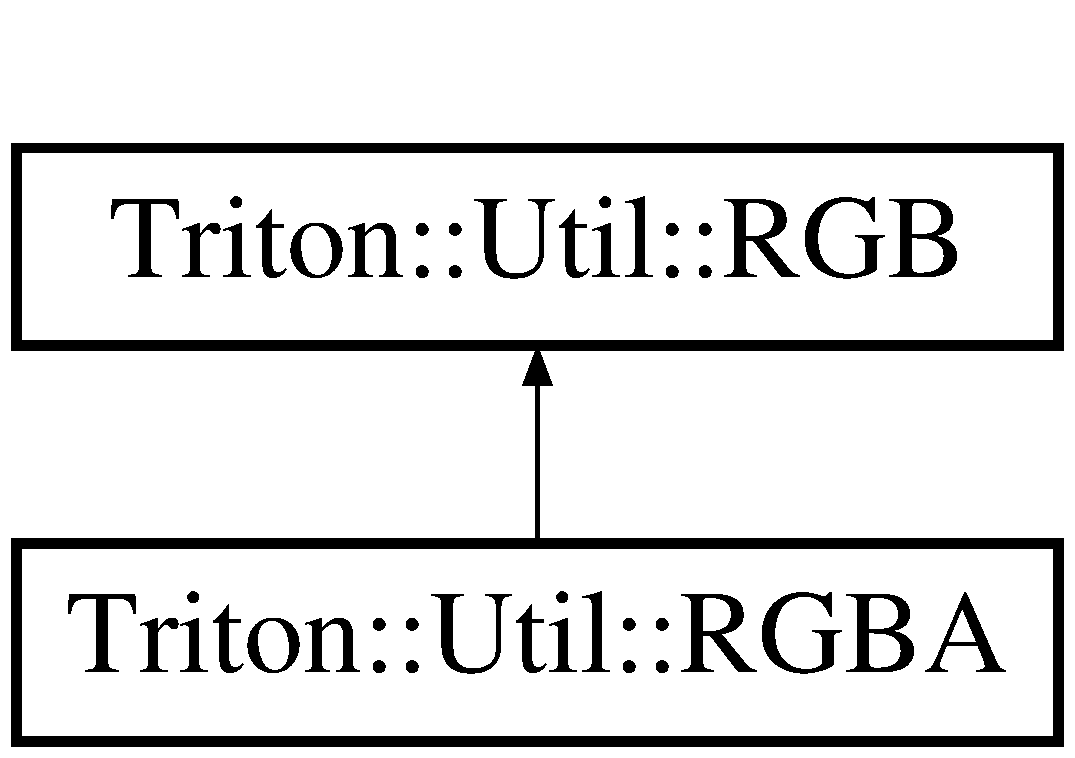
\includegraphics[height=2.000000cm]{struct_triton_1_1_util_1_1_r_g_b}
\end{center}
\end{figure}
\subsection*{Public Attributes}
\begin{DoxyCompactItemize}
\item 
const int \hyperlink{group__lus__color_ga25c01b9de0c18136b41333c426c2b226}{max} = 255
\item 
const int \hyperlink{group__lus__color_gaf4323053c0ecc091d206864ca2bbd26e}{min} = 0
\item 
unsigned short \hyperlink{group__lus__color_ga1fcfba2ad564a76d12f72f4b7441b3dc}{r}
\item 
unsigned short \hyperlink{group__lus__color_ga595248e981b342dfdeb08dc85f190229}{g}
\item 
unsigned short \hyperlink{group__lus__color_gadac238b0db4b4534cfa592331234b403}{b}
\end{DoxyCompactItemize}


\subsection{Detailed Description}
An rgb color object. 

Definition at line 13 of file color.\+h.



The documentation for this struct was generated from the following file\+:\begin{DoxyCompactItemize}
\item 
util/\hyperlink{color_8h}{color.\+h}\end{DoxyCompactItemize}

\hypertarget{struct_triton_1_1_util_1_1_r_g_b_a}{}\section{Triton\+:\+:Util\+:\+:R\+G\+B\+A Struct Reference}
\label{struct_triton_1_1_util_1_1_r_g_b_a}\index{Triton\+::\+Util\+::\+R\+G\+B\+A@{Triton\+::\+Util\+::\+R\+G\+B\+A}}


An \hyperlink{struct_triton_1_1_util_1_1_r_g_b}{R\+G\+B} object with Alpha.  




{\ttfamily \#include $<$color.\+h$>$}

Inheritance diagram for Triton\+:\+:Util\+:\+:R\+G\+B\+A\+:\begin{figure}[H]
\begin{center}
\leavevmode
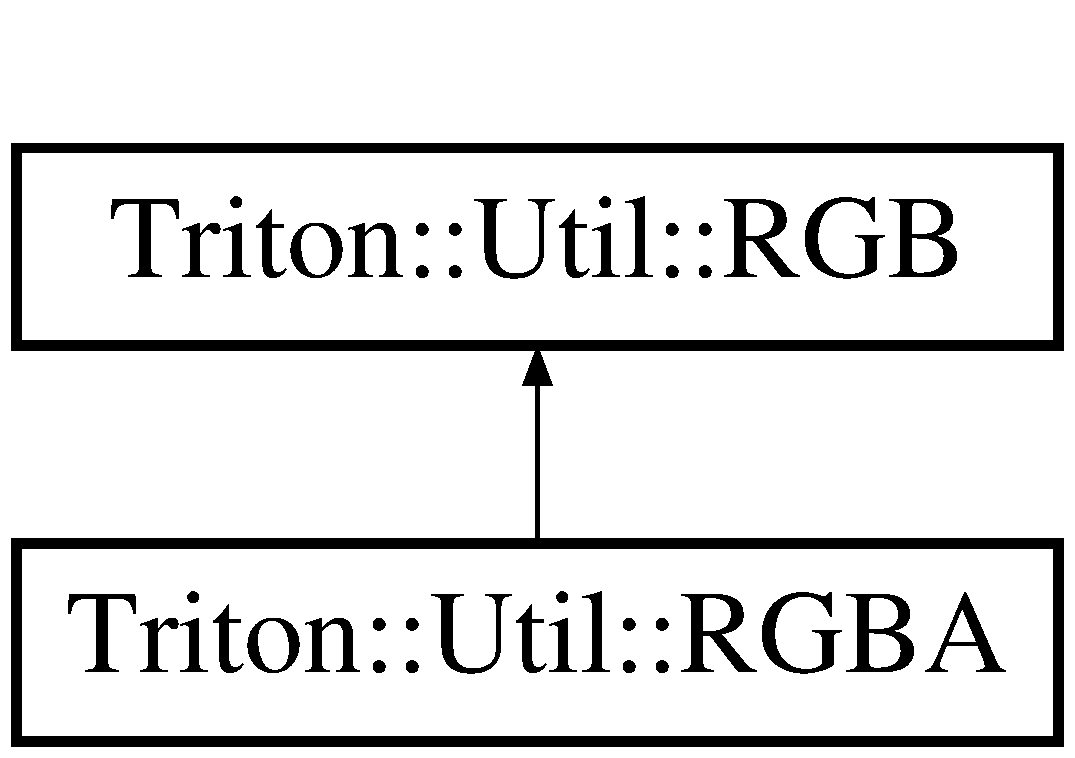
\includegraphics[height=2.000000cm]{struct_triton_1_1_util_1_1_r_g_b_a}
\end{center}
\end{figure}
\subsection*{Public Member Functions}
\begin{DoxyCompactItemize}
\item 
\hyperlink{group__lus__color_gad6fd5c4030e3b57842ca2b371e460e78}{R\+G\+B\+A} (unsigned short \hyperlink{group__lus__color_ga1fcfba2ad564a76d12f72f4b7441b3dc}{r}=0, unsigned short \hyperlink{group__lus__color_ga595248e981b342dfdeb08dc85f190229}{g}=0, unsigned short \hyperlink{group__lus__color_gadac238b0db4b4534cfa592331234b403}{b}=0, unsigned short \hyperlink{group__lus__color_ga91997be3ade022a459176810c8d2b777}{a}=\hyperlink{group__lus__color_ga25c01b9de0c18136b41333c426c2b226}{max})
\end{DoxyCompactItemize}
\subsection*{Public Attributes}
\begin{DoxyCompactItemize}
\item 
unsigned short \hyperlink{group__lus__color_ga91997be3ade022a459176810c8d2b777}{a}
\end{DoxyCompactItemize}


\subsection{Detailed Description}
An \hyperlink{struct_triton_1_1_util_1_1_r_g_b}{R\+G\+B} object with Alpha. 

Based on \hyperlink{struct_triton_1_1_util_1_1_r_g_b}{R\+G\+B} 

Definition at line 28 of file color.\+h.



The documentation for this struct was generated from the following file\+:\begin{DoxyCompactItemize}
\item 
util/\hyperlink{color_8h}{color.\+h}\end{DoxyCompactItemize}

\hypertarget{class_tri_1_1_graphic_1_1_shader}{}\section{Tri\+:\+:Graphic\+:\+:Shader Class Reference}
\label{class_tri_1_1_graphic_1_1_shader}\index{Tri\+::\+Graphic\+::\+Shader@{Tri\+::\+Graphic\+::\+Shader}}


{\ttfamily \#include $<$shader.\+h$>$}

\subsection*{Public Types}
\begin{DoxyCompactItemize}
\item 
enum \hyperlink{class_tri_1_1_graphic_1_1_shader_aeab62c54cc59f0c320f7472448afb97f}{Shader\+Type} \{ \hyperlink{class_tri_1_1_graphic_1_1_shader_aeab62c54cc59f0c320f7472448afb97fa458cb07d7027cb526382fee27325f51e}{V\+E\+R\+T\+E\+X} = 0, 
\hyperlink{class_tri_1_1_graphic_1_1_shader_aeab62c54cc59f0c320f7472448afb97fa101467f5fbf54bb0daf68342d966a92a}{G\+E\+O\+M\+E\+T\+R\+Y}, 
\hyperlink{class_tri_1_1_graphic_1_1_shader_aeab62c54cc59f0c320f7472448afb97faee1493bc20b88ace58506d1a9f97169e}{F\+R\+A\+G\+M\+E\+N\+T}, 
\hyperlink{class_tri_1_1_graphic_1_1_shader_aeab62c54cc59f0c320f7472448afb97fae499d59eee09b29b493bb14ae6a42b99}{S\+H\+A\+D\+E\+R\+\_\+\+T\+Y\+P\+E\+S\+\_\+\+L\+E\+N\+G\+T\+H}
 \}
\end{DoxyCompactItemize}
\subsection*{Public Member Functions}
\begin{DoxyCompactItemize}
\item 
\hyperlink{class_tri_1_1_graphic_1_1_shader_a504dce2ef14fa3843a515f7a9c80182a}{Shader} (Util\+::\+String src, \hyperlink{class_tri_1_1_graphic_1_1_shader_aeab62c54cc59f0c320f7472448afb97f}{Shader\+Type} type=\hyperlink{class_tri_1_1_graphic_1_1_shader_aeab62c54cc59f0c320f7472448afb97fa458cb07d7027cb526382fee27325f51e}{V\+E\+R\+T\+E\+X})
\item 
unsigned int \hyperlink{class_tri_1_1_graphic_1_1_shader_a56632c4d1caa2355f4493bdffac3b67c}{Get\+Id} ()
\item 
\hyperlink{class_tri_1_1_graphic_1_1_shader_aeab62c54cc59f0c320f7472448afb97f}{Shader\+Type} \hyperlink{class_tri_1_1_graphic_1_1_shader_a3c361810896a57041ad48f7cc3b9cfef}{Get\+Type} ()
\end{DoxyCompactItemize}


\subsection{Detailed Description}


Definition at line 25 of file shader.\+h.



\subsection{Member Enumeration Documentation}
\hypertarget{class_tri_1_1_graphic_1_1_shader_aeab62c54cc59f0c320f7472448afb97f}{}\index{Tri\+::\+Graphic\+::\+Shader@{Tri\+::\+Graphic\+::\+Shader}!Shader\+Type@{Shader\+Type}}
\index{Shader\+Type@{Shader\+Type}!Tri\+::\+Graphic\+::\+Shader@{Tri\+::\+Graphic\+::\+Shader}}
\subsubsection[{Shader\+Type}]{\setlength{\rightskip}{0pt plus 5cm}enum {\bf Tri\+::\+Graphic\+::\+Shader\+::\+Shader\+Type}}\label{class_tri_1_1_graphic_1_1_shader_aeab62c54cc59f0c320f7472448afb97f}
\begin{Desc}
\item[Enumerator]\par
\begin{description}
\index{V\+E\+R\+T\+E\+X@{V\+E\+R\+T\+E\+X}!Tri\+::\+Graphic\+::\+Shader@{Tri\+::\+Graphic\+::\+Shader}}\index{Tri\+::\+Graphic\+::\+Shader@{Tri\+::\+Graphic\+::\+Shader}!V\+E\+R\+T\+E\+X@{V\+E\+R\+T\+E\+X}}\item[{\em 
\hypertarget{class_tri_1_1_graphic_1_1_shader_aeab62c54cc59f0c320f7472448afb97fa458cb07d7027cb526382fee27325f51e}{}V\+E\+R\+T\+E\+X\label{class_tri_1_1_graphic_1_1_shader_aeab62c54cc59f0c320f7472448afb97fa458cb07d7027cb526382fee27325f51e}
}]\index{G\+E\+O\+M\+E\+T\+R\+Y@{G\+E\+O\+M\+E\+T\+R\+Y}!Tri\+::\+Graphic\+::\+Shader@{Tri\+::\+Graphic\+::\+Shader}}\index{Tri\+::\+Graphic\+::\+Shader@{Tri\+::\+Graphic\+::\+Shader}!G\+E\+O\+M\+E\+T\+R\+Y@{G\+E\+O\+M\+E\+T\+R\+Y}}\item[{\em 
\hypertarget{class_tri_1_1_graphic_1_1_shader_aeab62c54cc59f0c320f7472448afb97fa101467f5fbf54bb0daf68342d966a92a}{}G\+E\+O\+M\+E\+T\+R\+Y\label{class_tri_1_1_graphic_1_1_shader_aeab62c54cc59f0c320f7472448afb97fa101467f5fbf54bb0daf68342d966a92a}
}]\index{F\+R\+A\+G\+M\+E\+N\+T@{F\+R\+A\+G\+M\+E\+N\+T}!Tri\+::\+Graphic\+::\+Shader@{Tri\+::\+Graphic\+::\+Shader}}\index{Tri\+::\+Graphic\+::\+Shader@{Tri\+::\+Graphic\+::\+Shader}!F\+R\+A\+G\+M\+E\+N\+T@{F\+R\+A\+G\+M\+E\+N\+T}}\item[{\em 
\hypertarget{class_tri_1_1_graphic_1_1_shader_aeab62c54cc59f0c320f7472448afb97faee1493bc20b88ace58506d1a9f97169e}{}F\+R\+A\+G\+M\+E\+N\+T\label{class_tri_1_1_graphic_1_1_shader_aeab62c54cc59f0c320f7472448afb97faee1493bc20b88ace58506d1a9f97169e}
}]\index{S\+H\+A\+D\+E\+R\+\_\+\+T\+Y\+P\+E\+S\+\_\+\+L\+E\+N\+G\+T\+H@{S\+H\+A\+D\+E\+R\+\_\+\+T\+Y\+P\+E\+S\+\_\+\+L\+E\+N\+G\+T\+H}!Tri\+::\+Graphic\+::\+Shader@{Tri\+::\+Graphic\+::\+Shader}}\index{Tri\+::\+Graphic\+::\+Shader@{Tri\+::\+Graphic\+::\+Shader}!S\+H\+A\+D\+E\+R\+\_\+\+T\+Y\+P\+E\+S\+\_\+\+L\+E\+N\+G\+T\+H@{S\+H\+A\+D\+E\+R\+\_\+\+T\+Y\+P\+E\+S\+\_\+\+L\+E\+N\+G\+T\+H}}\item[{\em 
\hypertarget{class_tri_1_1_graphic_1_1_shader_aeab62c54cc59f0c320f7472448afb97fae499d59eee09b29b493bb14ae6a42b99}{}S\+H\+A\+D\+E\+R\+\_\+\+T\+Y\+P\+E\+S\+\_\+\+L\+E\+N\+G\+T\+H\label{class_tri_1_1_graphic_1_1_shader_aeab62c54cc59f0c320f7472448afb97fae499d59eee09b29b493bb14ae6a42b99}
}]\end{description}
\end{Desc}


Definition at line 30 of file shader.\+h.



\subsection{Constructor \& Destructor Documentation}
\hypertarget{class_tri_1_1_graphic_1_1_shader_a504dce2ef14fa3843a515f7a9c80182a}{}\index{Tri\+::\+Graphic\+::\+Shader@{Tri\+::\+Graphic\+::\+Shader}!Shader@{Shader}}
\index{Shader@{Shader}!Tri\+::\+Graphic\+::\+Shader@{Tri\+::\+Graphic\+::\+Shader}}
\subsubsection[{Shader}]{\setlength{\rightskip}{0pt plus 5cm}Tri\+::\+Graphic\+::\+Shader\+::\+Shader (
\begin{DoxyParamCaption}
\item[{Util\+::\+String}]{src, }
\item[{{\bf Shader\+Type}}]{type = {\ttfamily {\bf V\+E\+R\+T\+E\+X}}}
\end{DoxyParamCaption}
)}\label{class_tri_1_1_graphic_1_1_shader_a504dce2ef14fa3843a515f7a9c80182a}


\subsection{Member Function Documentation}
\hypertarget{class_tri_1_1_graphic_1_1_shader_a56632c4d1caa2355f4493bdffac3b67c}{}\index{Tri\+::\+Graphic\+::\+Shader@{Tri\+::\+Graphic\+::\+Shader}!Get\+Id@{Get\+Id}}
\index{Get\+Id@{Get\+Id}!Tri\+::\+Graphic\+::\+Shader@{Tri\+::\+Graphic\+::\+Shader}}
\subsubsection[{Get\+Id}]{\setlength{\rightskip}{0pt plus 5cm}unsigned int Tri\+::\+Graphic\+::\+Shader\+::\+Get\+Id (
\begin{DoxyParamCaption}
{}
\end{DoxyParamCaption}
)}\label{class_tri_1_1_graphic_1_1_shader_a56632c4d1caa2355f4493bdffac3b67c}
\hypertarget{class_tri_1_1_graphic_1_1_shader_a3c361810896a57041ad48f7cc3b9cfef}{}\index{Tri\+::\+Graphic\+::\+Shader@{Tri\+::\+Graphic\+::\+Shader}!Get\+Type@{Get\+Type}}
\index{Get\+Type@{Get\+Type}!Tri\+::\+Graphic\+::\+Shader@{Tri\+::\+Graphic\+::\+Shader}}
\subsubsection[{Get\+Type}]{\setlength{\rightskip}{0pt plus 5cm}{\bf Shader\+Type} Tri\+::\+Graphic\+::\+Shader\+::\+Get\+Type (
\begin{DoxyParamCaption}
{}
\end{DoxyParamCaption}
)}\label{class_tri_1_1_graphic_1_1_shader_a3c361810896a57041ad48f7cc3b9cfef}


The documentation for this class was generated from the following file\+:\begin{DoxyCompactItemize}
\item 
graphic/\hyperlink{shader_8h}{shader.\+h}\end{DoxyCompactItemize}

\hypertarget{class_tri_1_1_graphic_1_1_shader_program}{}\section{Tri\+:\+:Graphic\+:\+:Shader\+Program Class Reference}
\label{class_tri_1_1_graphic_1_1_shader_program}\index{Tri\+::\+Graphic\+::\+Shader\+Program@{Tri\+::\+Graphic\+::\+Shader\+Program}}


{\ttfamily \#include $<$shader.\+h$>$}

\subsection*{Public Member Functions}
\begin{DoxyCompactItemize}
\item 
\hyperlink{class_tri_1_1_graphic_1_1_shader_program_acee0f1e112a1dddbdcda4e640c32eea5}{Shader\+Program} ()
\item 
bool \hyperlink{class_tri_1_1_graphic_1_1_shader_program_a8712f06282104ecd3bf25faa915c9e9d}{Assign\+Shader} (\hyperlink{class_tri_1_1_graphic_1_1_shader}{Shader} $\ast$shader)
\item 
void \hyperlink{class_tri_1_1_graphic_1_1_shader_program_a8661a9f4836c4783e101a8333d0d537e}{Load\+Uniform} (Util\+::\+String name)
\item 
unsigned int \hyperlink{class_tri_1_1_graphic_1_1_shader_program_afc4dd0cd5b38396039b2ceec84e841ae}{Get\+Id} ()
\item 
\hyperlink{class_tri_1_1_graphic_1_1_shader_program_a5042c8137c4e543c26163b934e122392}{$\sim$\+Shader\+Program} ()
\end{DoxyCompactItemize}


\subsection{Detailed Description}


Definition at line 44 of file shader.\+h.



\subsection{Constructor \& Destructor Documentation}
\hypertarget{class_tri_1_1_graphic_1_1_shader_program_acee0f1e112a1dddbdcda4e640c32eea5}{}\index{Tri\+::\+Graphic\+::\+Shader\+Program@{Tri\+::\+Graphic\+::\+Shader\+Program}!Shader\+Program@{Shader\+Program}}
\index{Shader\+Program@{Shader\+Program}!Tri\+::\+Graphic\+::\+Shader\+Program@{Tri\+::\+Graphic\+::\+Shader\+Program}}
\subsubsection[{Shader\+Program}]{\setlength{\rightskip}{0pt plus 5cm}Tri\+::\+Graphic\+::\+Shader\+Program\+::\+Shader\+Program (
\begin{DoxyParamCaption}
{}
\end{DoxyParamCaption}
)}\label{class_tri_1_1_graphic_1_1_shader_program_acee0f1e112a1dddbdcda4e640c32eea5}
\hypertarget{class_tri_1_1_graphic_1_1_shader_program_a5042c8137c4e543c26163b934e122392}{}\index{Tri\+::\+Graphic\+::\+Shader\+Program@{Tri\+::\+Graphic\+::\+Shader\+Program}!````~Shader\+Program@{$\sim$\+Shader\+Program}}
\index{````~Shader\+Program@{$\sim$\+Shader\+Program}!Tri\+::\+Graphic\+::\+Shader\+Program@{Tri\+::\+Graphic\+::\+Shader\+Program}}
\subsubsection[{$\sim$\+Shader\+Program}]{\setlength{\rightskip}{0pt plus 5cm}Tri\+::\+Graphic\+::\+Shader\+Program\+::$\sim$\+Shader\+Program (
\begin{DoxyParamCaption}
{}
\end{DoxyParamCaption}
)}\label{class_tri_1_1_graphic_1_1_shader_program_a5042c8137c4e543c26163b934e122392}


\subsection{Member Function Documentation}
\hypertarget{class_tri_1_1_graphic_1_1_shader_program_a8712f06282104ecd3bf25faa915c9e9d}{}\index{Tri\+::\+Graphic\+::\+Shader\+Program@{Tri\+::\+Graphic\+::\+Shader\+Program}!Assign\+Shader@{Assign\+Shader}}
\index{Assign\+Shader@{Assign\+Shader}!Tri\+::\+Graphic\+::\+Shader\+Program@{Tri\+::\+Graphic\+::\+Shader\+Program}}
\subsubsection[{Assign\+Shader}]{\setlength{\rightskip}{0pt plus 5cm}bool Tri\+::\+Graphic\+::\+Shader\+Program\+::\+Assign\+Shader (
\begin{DoxyParamCaption}
\item[{{\bf Shader} $\ast$}]{shader}
\end{DoxyParamCaption}
)}\label{class_tri_1_1_graphic_1_1_shader_program_a8712f06282104ecd3bf25faa915c9e9d}
\hypertarget{class_tri_1_1_graphic_1_1_shader_program_afc4dd0cd5b38396039b2ceec84e841ae}{}\index{Tri\+::\+Graphic\+::\+Shader\+Program@{Tri\+::\+Graphic\+::\+Shader\+Program}!Get\+Id@{Get\+Id}}
\index{Get\+Id@{Get\+Id}!Tri\+::\+Graphic\+::\+Shader\+Program@{Tri\+::\+Graphic\+::\+Shader\+Program}}
\subsubsection[{Get\+Id}]{\setlength{\rightskip}{0pt plus 5cm}unsigned int Tri\+::\+Graphic\+::\+Shader\+Program\+::\+Get\+Id (
\begin{DoxyParamCaption}
{}
\end{DoxyParamCaption}
)}\label{class_tri_1_1_graphic_1_1_shader_program_afc4dd0cd5b38396039b2ceec84e841ae}
\hypertarget{class_tri_1_1_graphic_1_1_shader_program_a8661a9f4836c4783e101a8333d0d537e}{}\index{Tri\+::\+Graphic\+::\+Shader\+Program@{Tri\+::\+Graphic\+::\+Shader\+Program}!Load\+Uniform@{Load\+Uniform}}
\index{Load\+Uniform@{Load\+Uniform}!Tri\+::\+Graphic\+::\+Shader\+Program@{Tri\+::\+Graphic\+::\+Shader\+Program}}
\subsubsection[{Load\+Uniform}]{\setlength{\rightskip}{0pt plus 5cm}void Tri\+::\+Graphic\+::\+Shader\+Program\+::\+Load\+Uniform (
\begin{DoxyParamCaption}
\item[{Util\+::\+String}]{name}
\end{DoxyParamCaption}
)}\label{class_tri_1_1_graphic_1_1_shader_program_a8661a9f4836c4783e101a8333d0d537e}


The documentation for this class was generated from the following file\+:\begin{DoxyCompactItemize}
\item 
graphic/\hyperlink{shader_8h}{shader.\+h}\end{DoxyCompactItemize}

\hypertarget{class_leak_1_1_audio_1_1_sound}{}\section{Leak\+:\+:Audio\+:\+:Sound Class Reference}
\label{class_leak_1_1_audio_1_1_sound}\index{Leak\+::\+Audio\+::\+Sound@{Leak\+::\+Audio\+::\+Sound}}


{\ttfamily \#include $<$sound.\+h$>$}



\subsection{Detailed Description}


Definition at line 9 of file sound.\+h.



The documentation for this class was generated from the following file\+:\begin{DoxyCompactItemize}
\item 
audio/\hyperlink{sound_8h}{sound.\+h}\end{DoxyCompactItemize}

\hypertarget{class_tri_1_1_graphic_1_1_text}{}\section{Tri\+:\+:Graphic\+:\+:Text Class Reference}
\label{class_tri_1_1_graphic_1_1_text}\index{Tri\+::\+Graphic\+::\+Text@{Tri\+::\+Graphic\+::\+Text}}


{\ttfamily \#include $<$render.\+h$>$}

Inheritance diagram for Tri\+:\+:Graphic\+:\+:Text\+:\begin{figure}[H]
\begin{center}
\leavevmode
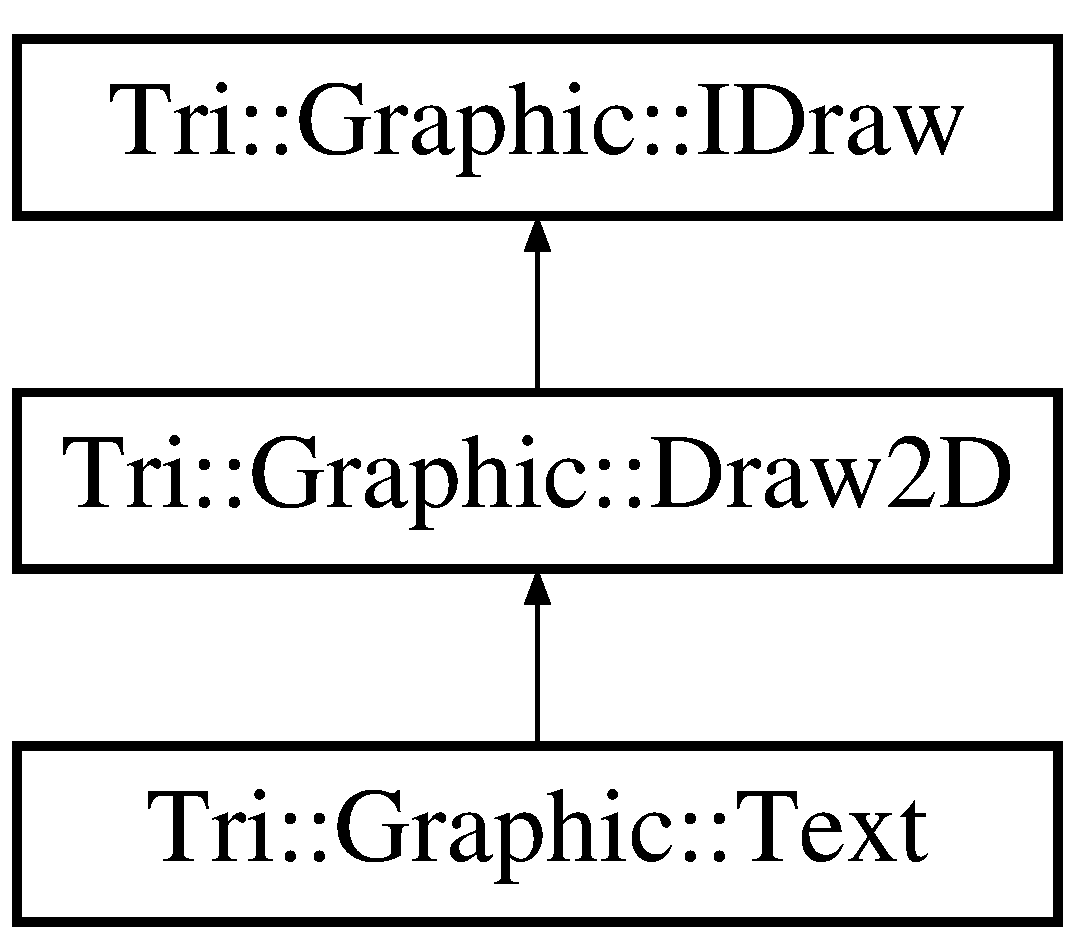
\includegraphics[height=3.000000cm]{class_tri_1_1_graphic_1_1_text}
\end{center}
\end{figure}
\subsection*{Public Member Functions}
\begin{DoxyCompactItemize}
\item 
\hyperlink{class_tri_1_1_graphic_1_1_text_a9854bdf2b097ae80215a8bfb1091bc9f}{Text} (Resource\+::\+Image texture)
\item 
\hyperlink{class_tri_1_1_graphic_1_1_text_a6e1854c52245f12ed44b65a8e27522c6}{Text} (const Util\+::\+String \&s, Resource\+::\+Image texture)
\item 
\hyperlink{class_tri_1_1_graphic_1_1_text_ae722b27dcdbdb07de73b218334b7c8a4}{Text} (const Util\+::\+String \&s, std\+::size\+\_\+t n, Resource\+::\+Image texture)
\item 
\hyperlink{class_tri_1_1_graphic_1_1_text_a6e01d3380be722b59da66a056c448671}{Text} (const char $\ast$s, std\+::size\+\_\+t n, Resource\+::\+Image texture)
\item 
\hyperlink{class_tri_1_1_graphic_1_1_text_a9a8d37cc5cc578d322aecf1a50b7f207}{Text} (const char $\ast$s, Resource\+::\+Image texture)
\item 
\hyperlink{class_tri_1_1_graphic_1_1_text_ab453c7ed9348c3f3d0f86e10c2fa8652}{Text} (std\+::size\+\_\+t n, char c, Resource\+::\+Image texture)
\item 
{\footnotesize template$<$class Input\+Iterator $>$ }\\\hyperlink{class_tri_1_1_graphic_1_1_text_a33c5dd1e43a3356b2f973e7f28362a87}{Text} (Input\+Iterator first, Input\+Iterator last, Resource\+::\+Image texture)
\end{DoxyCompactItemize}
\subsection*{Public Attributes}
\begin{DoxyCompactItemize}
\item 
Util\+::\+String \hyperlink{class_tri_1_1_graphic_1_1_text_ab9700e2f9b6592ffcab3453c95c06152}{text}
\end{DoxyCompactItemize}
\subsection*{Additional Inherited Members}


\subsection{Detailed Description}
A small class for rendering text from Util\+::\+String and a Resource\+::\+Image font

All input is updated on-\/the-\/fly

Example of use\+: 
\begin{DoxyCode}
Tri::Graphic::Render::Text txt(fontImage, \textcolor{stringliteral}{"Foo"});
txt.text = \textcolor{stringliteral}{"Bar"} \textcolor{comment}{// txt now displays Bar instead of Foo}
\end{DoxyCode}
 

Definition at line 133 of file render.\+h.



\subsection{Constructor \& Destructor Documentation}
\hypertarget{class_tri_1_1_graphic_1_1_text_a9854bdf2b097ae80215a8bfb1091bc9f}{}\index{Tri\+::\+Graphic\+::\+Text@{Tri\+::\+Graphic\+::\+Text}!Text@{Text}}
\index{Text@{Text}!Tri\+::\+Graphic\+::\+Text@{Tri\+::\+Graphic\+::\+Text}}
\subsubsection[{Text}]{\setlength{\rightskip}{0pt plus 5cm}Tri\+::\+Graphic\+::\+Text\+::\+Text (
\begin{DoxyParamCaption}
\item[{Resource\+::\+Image}]{texture}
\end{DoxyParamCaption}
)\hspace{0.3cm}{\ttfamily [inline]}}\label{class_tri_1_1_graphic_1_1_text_a9854bdf2b097ae80215a8bfb1091bc9f}


Definition at line 137 of file render.\+h.

\hypertarget{class_tri_1_1_graphic_1_1_text_a6e1854c52245f12ed44b65a8e27522c6}{}\index{Tri\+::\+Graphic\+::\+Text@{Tri\+::\+Graphic\+::\+Text}!Text@{Text}}
\index{Text@{Text}!Tri\+::\+Graphic\+::\+Text@{Tri\+::\+Graphic\+::\+Text}}
\subsubsection[{Text}]{\setlength{\rightskip}{0pt plus 5cm}Tri\+::\+Graphic\+::\+Text\+::\+Text (
\begin{DoxyParamCaption}
\item[{const Util\+::\+String \&}]{s, }
\item[{Resource\+::\+Image}]{texture}
\end{DoxyParamCaption}
)\hspace{0.3cm}{\ttfamily [inline]}}\label{class_tri_1_1_graphic_1_1_text_a6e1854c52245f12ed44b65a8e27522c6}


Definition at line 138 of file render.\+h.

\hypertarget{class_tri_1_1_graphic_1_1_text_ae722b27dcdbdb07de73b218334b7c8a4}{}\index{Tri\+::\+Graphic\+::\+Text@{Tri\+::\+Graphic\+::\+Text}!Text@{Text}}
\index{Text@{Text}!Tri\+::\+Graphic\+::\+Text@{Tri\+::\+Graphic\+::\+Text}}
\subsubsection[{Text}]{\setlength{\rightskip}{0pt plus 5cm}Tri\+::\+Graphic\+::\+Text\+::\+Text (
\begin{DoxyParamCaption}
\item[{const Util\+::\+String \&}]{s, }
\item[{std\+::size\+\_\+t}]{n, }
\item[{Resource\+::\+Image}]{texture}
\end{DoxyParamCaption}
)\hspace{0.3cm}{\ttfamily [inline]}}\label{class_tri_1_1_graphic_1_1_text_ae722b27dcdbdb07de73b218334b7c8a4}


Definition at line 139 of file render.\+h.

\hypertarget{class_tri_1_1_graphic_1_1_text_a6e01d3380be722b59da66a056c448671}{}\index{Tri\+::\+Graphic\+::\+Text@{Tri\+::\+Graphic\+::\+Text}!Text@{Text}}
\index{Text@{Text}!Tri\+::\+Graphic\+::\+Text@{Tri\+::\+Graphic\+::\+Text}}
\subsubsection[{Text}]{\setlength{\rightskip}{0pt plus 5cm}Tri\+::\+Graphic\+::\+Text\+::\+Text (
\begin{DoxyParamCaption}
\item[{const char $\ast$}]{s, }
\item[{std\+::size\+\_\+t}]{n, }
\item[{Resource\+::\+Image}]{texture}
\end{DoxyParamCaption}
)\hspace{0.3cm}{\ttfamily [inline]}}\label{class_tri_1_1_graphic_1_1_text_a6e01d3380be722b59da66a056c448671}


Definition at line 140 of file render.\+h.

\hypertarget{class_tri_1_1_graphic_1_1_text_a9a8d37cc5cc578d322aecf1a50b7f207}{}\index{Tri\+::\+Graphic\+::\+Text@{Tri\+::\+Graphic\+::\+Text}!Text@{Text}}
\index{Text@{Text}!Tri\+::\+Graphic\+::\+Text@{Tri\+::\+Graphic\+::\+Text}}
\subsubsection[{Text}]{\setlength{\rightskip}{0pt plus 5cm}Tri\+::\+Graphic\+::\+Text\+::\+Text (
\begin{DoxyParamCaption}
\item[{const char $\ast$}]{s, }
\item[{Resource\+::\+Image}]{texture}
\end{DoxyParamCaption}
)\hspace{0.3cm}{\ttfamily [inline]}}\label{class_tri_1_1_graphic_1_1_text_a9a8d37cc5cc578d322aecf1a50b7f207}


Definition at line 141 of file render.\+h.

\hypertarget{class_tri_1_1_graphic_1_1_text_ab453c7ed9348c3f3d0f86e10c2fa8652}{}\index{Tri\+::\+Graphic\+::\+Text@{Tri\+::\+Graphic\+::\+Text}!Text@{Text}}
\index{Text@{Text}!Tri\+::\+Graphic\+::\+Text@{Tri\+::\+Graphic\+::\+Text}}
\subsubsection[{Text}]{\setlength{\rightskip}{0pt plus 5cm}Tri\+::\+Graphic\+::\+Text\+::\+Text (
\begin{DoxyParamCaption}
\item[{std\+::size\+\_\+t}]{n, }
\item[{char}]{c, }
\item[{Resource\+::\+Image}]{texture}
\end{DoxyParamCaption}
)\hspace{0.3cm}{\ttfamily [inline]}}\label{class_tri_1_1_graphic_1_1_text_ab453c7ed9348c3f3d0f86e10c2fa8652}


Definition at line 142 of file render.\+h.

\hypertarget{class_tri_1_1_graphic_1_1_text_a33c5dd1e43a3356b2f973e7f28362a87}{}\index{Tri\+::\+Graphic\+::\+Text@{Tri\+::\+Graphic\+::\+Text}!Text@{Text}}
\index{Text@{Text}!Tri\+::\+Graphic\+::\+Text@{Tri\+::\+Graphic\+::\+Text}}
\subsubsection[{Text}]{\setlength{\rightskip}{0pt plus 5cm}template$<$class Input\+Iterator $>$ Tri\+::\+Graphic\+::\+Text\+::\+Text (
\begin{DoxyParamCaption}
\item[{Input\+Iterator}]{first, }
\item[{Input\+Iterator}]{last, }
\item[{Resource\+::\+Image}]{texture}
\end{DoxyParamCaption}
)\hspace{0.3cm}{\ttfamily [inline]}}\label{class_tri_1_1_graphic_1_1_text_a33c5dd1e43a3356b2f973e7f28362a87}


Definition at line 144 of file render.\+h.



\subsection{Member Data Documentation}
\hypertarget{class_tri_1_1_graphic_1_1_text_ab9700e2f9b6592ffcab3453c95c06152}{}\index{Tri\+::\+Graphic\+::\+Text@{Tri\+::\+Graphic\+::\+Text}!text@{text}}
\index{text@{text}!Tri\+::\+Graphic\+::\+Text@{Tri\+::\+Graphic\+::\+Text}}
\subsubsection[{text}]{\setlength{\rightskip}{0pt plus 5cm}Util\+::\+String Tri\+::\+Graphic\+::\+Text\+::text}\label{class_tri_1_1_graphic_1_1_text_ab9700e2f9b6592ffcab3453c95c06152}


Definition at line 136 of file render.\+h.



The documentation for this class was generated from the following file\+:\begin{DoxyCompactItemize}
\item 
graphic/\hyperlink{render_8h}{render.\+h}\end{DoxyCompactItemize}

\hypertarget{class_tri_1_1_graphic_1_1_uniform}{}\section{Tri\+:\+:Graphic\+:\+:Uniform Class Reference}
\label{class_tri_1_1_graphic_1_1_uniform}\index{Tri\+::\+Graphic\+::\+Uniform@{Tri\+::\+Graphic\+::\+Uniform}}


{\ttfamily \#include $<$shader.\+h$>$}

\subsection*{Public Member Functions}
\begin{DoxyCompactItemize}
\item 
Util\+::\+String \hyperlink{class_tri_1_1_graphic_1_1_uniform_a5d66ced6c1de8c7d5cd5e6cd5fb221b8}{Get\+Name} ()
\item 
unsigned int \hyperlink{class_tri_1_1_graphic_1_1_uniform_a222f85be09d5892ce0e1c91617d035b2}{Get\+Id} ()
\end{DoxyCompactItemize}
\subsection*{Friends}
\begin{DoxyCompactItemize}
\item 
class \hyperlink{class_tri_1_1_graphic_1_1_uniform_aef20119bde6aff11ffd23f3ea2131b86}{Shader\+Program}
\end{DoxyCompactItemize}


\subsection{Detailed Description}


Definition at line 12 of file shader.\+h.



\subsection{Member Function Documentation}
\hypertarget{class_tri_1_1_graphic_1_1_uniform_a222f85be09d5892ce0e1c91617d035b2}{}\index{Tri\+::\+Graphic\+::\+Uniform@{Tri\+::\+Graphic\+::\+Uniform}!Get\+Id@{Get\+Id}}
\index{Get\+Id@{Get\+Id}!Tri\+::\+Graphic\+::\+Uniform@{Tri\+::\+Graphic\+::\+Uniform}}
\subsubsection[{Get\+Id}]{\setlength{\rightskip}{0pt plus 5cm}unsigned int Tri\+::\+Graphic\+::\+Uniform\+::\+Get\+Id (
\begin{DoxyParamCaption}
{}
\end{DoxyParamCaption}
)}\label{class_tri_1_1_graphic_1_1_uniform_a222f85be09d5892ce0e1c91617d035b2}
\hypertarget{class_tri_1_1_graphic_1_1_uniform_a5d66ced6c1de8c7d5cd5e6cd5fb221b8}{}\index{Tri\+::\+Graphic\+::\+Uniform@{Tri\+::\+Graphic\+::\+Uniform}!Get\+Name@{Get\+Name}}
\index{Get\+Name@{Get\+Name}!Tri\+::\+Graphic\+::\+Uniform@{Tri\+::\+Graphic\+::\+Uniform}}
\subsubsection[{Get\+Name}]{\setlength{\rightskip}{0pt plus 5cm}Util\+::\+String Tri\+::\+Graphic\+::\+Uniform\+::\+Get\+Name (
\begin{DoxyParamCaption}
{}
\end{DoxyParamCaption}
)}\label{class_tri_1_1_graphic_1_1_uniform_a5d66ced6c1de8c7d5cd5e6cd5fb221b8}


\subsection{Friends And Related Function Documentation}
\hypertarget{class_tri_1_1_graphic_1_1_uniform_aef20119bde6aff11ffd23f3ea2131b86}{}\index{Tri\+::\+Graphic\+::\+Uniform@{Tri\+::\+Graphic\+::\+Uniform}!Shader\+Program@{Shader\+Program}}
\index{Shader\+Program@{Shader\+Program}!Tri\+::\+Graphic\+::\+Uniform@{Tri\+::\+Graphic\+::\+Uniform}}
\subsubsection[{Shader\+Program}]{\setlength{\rightskip}{0pt plus 5cm}friend class {\bf Shader\+Program}\hspace{0.3cm}{\ttfamily [friend]}}\label{class_tri_1_1_graphic_1_1_uniform_aef20119bde6aff11ffd23f3ea2131b86}


Definition at line 14 of file shader.\+h.



The documentation for this class was generated from the following file\+:\begin{DoxyCompactItemize}
\item 
graphic/\hyperlink{shader_8h}{shader.\+h}\end{DoxyCompactItemize}

\hypertarget{class_triton_1_1_util_1_1_vector1}{}\section{Triton\+:\+:Util\+:\+:Vector1$<$ T $>$ Class Template Reference}
\label{class_triton_1_1_util_1_1_vector1}\index{Triton\+::\+Util\+::\+Vector1$<$ T $>$@{Triton\+::\+Util\+::\+Vector1$<$ T $>$}}


Utility template class to store and manipulate 1-\/dimensional vector positions.  




{\ttfamily \#include $<$Vector1.\+hpp$>$}

Inheritance diagram for Triton\+:\+:Util\+:\+:Vector1$<$ T $>$\+:\begin{figure}[H]
\begin{center}
\leavevmode
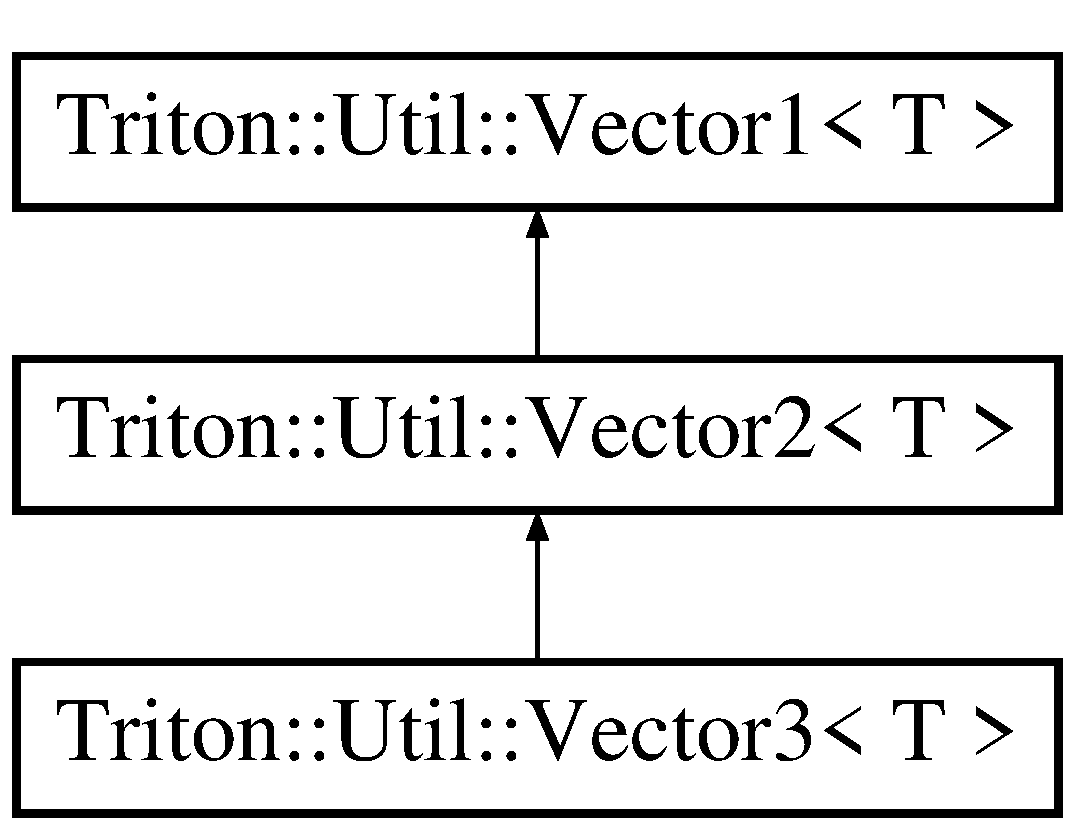
\includegraphics[height=3.000000cm]{class_triton_1_1_util_1_1_vector1}
\end{center}
\end{figure}
\subsection*{Public Member Functions}
\begin{DoxyCompactItemize}
\item 
\hyperlink{class_triton_1_1_util_1_1_vector1_a81f8a873ba7e16edb941462a85f8a0bb}{Vector1} (T X=0)
\begin{DoxyCompactList}\small\item\em Construct the vector from its coordinates. \end{DoxyCompactList}\item 
{\footnotesize template$<$typename U $>$ }\\\hyperlink{class_triton_1_1_util_1_1_vector1_a1f1f214d93a14d95418bf415c134def7}{Vector1} (const \hyperlink{class_triton_1_1_util_1_1_vector1}{Vector1}$<$ U $>$ \&vector)
\begin{DoxyCompactList}\small\item\em Construct the vector from another type of vector. \end{DoxyCompactList}\item 
{\footnotesize template$<$typename U $>$ }\\\hyperlink{class_triton_1_1_util_1_1_vector1}{Vector1}$<$ T $>$ \hyperlink{class_triton_1_1_util_1_1_vector1_a01811cae3774b28871bf3c54cd22f040}{distance} (\hyperlink{class_triton_1_1_util_1_1_vector1}{Vector1}$<$ U $>$ vector)
\begin{DoxyCompactList}\small\item\em Returns a vector that holds the distance between this and vector. \end{DoxyCompactList}\item 
\hyperlink{class_triton_1_1_util_1_1_vector1}{Vector1}$<$ T $>$ \hyperlink{class_triton_1_1_util_1_1_vector1_a96679ffc24e262cf49db8f30c887352e}{abs\+V} ()
\begin{DoxyCompactList}\small\item\em Constructs a \hyperlink{class_triton_1_1_util_1_1_vector1}{Triton\+::\+Util\+::\+Vector1} with an absolute value of this vector. \end{DoxyCompactList}\item 
virtual T \hyperlink{class_triton_1_1_util_1_1_vector1_a5b0223acf46ae3ac6afd60bdea748bbf}{operator\mbox{[}$\,$\mbox{]}} (int index)
\begin{DoxyCompactList}\small\item\em A safe and cross-\/object way of calling the member variables. \end{DoxyCompactList}\end{DoxyCompactItemize}
\subsection*{Public Attributes}
\begin{DoxyCompactItemize}
\item 
T \hyperlink{class_triton_1_1_util_1_1_vector1_a379cb608c766a1eed8f730fcff9dff9c}{m\+\_\+\+X\+Position}
\begin{DoxyCompactList}\small\item\em Y coordinate of the vector. \end{DoxyCompactList}\end{DoxyCompactItemize}
\subsection*{Related Functions}
(Note that these are not member functions.) \begin{DoxyCompactItemize}
\item 
{\footnotesize template$<$typename T $>$ }\\\hyperlink{class_triton_1_1_util_1_1_vector1}{Vector1}$<$ T $>$ \hyperlink{class_triton_1_1_util_1_1_vector1_aaebf92e5156895243d79dd4aba7ef0fd}{operator-\/} (const \hyperlink{class_triton_1_1_util_1_1_vector1}{Vector1}$<$ T $>$ \&left)
\begin{DoxyCompactList}\small\item\em Overload of unary operator -\/. \end{DoxyCompactList}\item 
{\footnotesize template$<$typename T $>$ }\\\hyperlink{class_triton_1_1_util_1_1_vector1}{Vector1}$<$ T $>$ \& \hyperlink{class_triton_1_1_util_1_1_vector1_a56697d34ba8f3f1132471876cb7ba3be}{operator+=} (\hyperlink{class_triton_1_1_util_1_1_vector1}{Vector1}$<$ T $>$ \&left, const \hyperlink{class_triton_1_1_util_1_1_vector1}{Vector1}$<$ T $>$ \&right)
\begin{DoxyCompactList}\small\item\em Overload of binary operator +=. \end{DoxyCompactList}\item 
{\footnotesize template$<$typename T $>$ }\\\hyperlink{class_triton_1_1_util_1_1_vector1}{Vector1}$<$ T $>$ \& \hyperlink{class_triton_1_1_util_1_1_vector1_a2073f04ccc39763a6baad165805d78a2}{operator-\/=} (\hyperlink{class_triton_1_1_util_1_1_vector1}{Vector1}$<$ T $>$ \&left, const \hyperlink{class_triton_1_1_util_1_1_vector1}{Vector1}$<$ T $>$ \&right)
\begin{DoxyCompactList}\small\item\em Overload of binary operator -\/=. \end{DoxyCompactList}\item 
{\footnotesize template$<$typename T $>$ }\\\hyperlink{class_triton_1_1_util_1_1_vector1}{Vector1}$<$ T $>$ \hyperlink{class_triton_1_1_util_1_1_vector1_a6874d414ce5ae0a31cc2891cf212b6c4}{operator+} (const \hyperlink{class_triton_1_1_util_1_1_vector1}{Vector1}$<$ T $>$ \&left, const \hyperlink{class_triton_1_1_util_1_1_vector1}{Vector1}$<$ T $>$ \&right)
\begin{DoxyCompactList}\small\item\em Overload of binary operator +. \end{DoxyCompactList}\item 
{\footnotesize template$<$typename T $>$ }\\\hyperlink{class_triton_1_1_util_1_1_vector1}{Vector1}$<$ T $>$ \hyperlink{class_triton_1_1_util_1_1_vector1_a1094f567d2865ee5d36ce22bde608260}{operator-\/} (const \hyperlink{class_triton_1_1_util_1_1_vector1}{Vector1}$<$ T $>$ \&left, const \hyperlink{class_triton_1_1_util_1_1_vector1}{Vector1}$<$ T $>$ \&right)
\begin{DoxyCompactList}\small\item\em Overload of binary operator -\/. \end{DoxyCompactList}\item 
{\footnotesize template$<$typename T $>$ }\\\hyperlink{class_triton_1_1_util_1_1_vector1}{Vector1}$<$ T $>$ \hyperlink{class_triton_1_1_util_1_1_vector1_ab1b522600e6551482ead1a3030bae02b}{operator$\ast$} (const \hyperlink{class_triton_1_1_util_1_1_vector1}{Vector1}$<$ T $>$ \&left, T right)
\begin{DoxyCompactList}\small\item\em Overload of binary operator $\ast$. \end{DoxyCompactList}\item 
{\footnotesize template$<$typename T $>$ }\\\hyperlink{class_triton_1_1_util_1_1_vector1}{Vector1}$<$ T $>$ \hyperlink{class_triton_1_1_util_1_1_vector1_a32665d4805eabc6a1b57c8c8313ec520}{operator$\ast$} (T left, const \hyperlink{class_triton_1_1_util_1_1_vector1}{Vector1}$<$ T $>$ \&right)
\begin{DoxyCompactList}\small\item\em Overload of binary operator $\ast$. \end{DoxyCompactList}\item 
{\footnotesize template$<$typename T $>$ }\\\hyperlink{class_triton_1_1_util_1_1_vector1}{Vector1}$<$ T $>$ \& \hyperlink{class_triton_1_1_util_1_1_vector1_ae8263e2fa81292823605129b52c3484a}{operator$\ast$=} (\hyperlink{class_triton_1_1_util_1_1_vector1}{Vector1}$<$ T $>$ \&left, T right)
\begin{DoxyCompactList}\small\item\em Overload of binary operator $\ast$=. \end{DoxyCompactList}\item 
{\footnotesize template$<$typename T $>$ }\\\hyperlink{class_triton_1_1_util_1_1_vector1}{Vector1}$<$ T $>$ \hyperlink{class_triton_1_1_util_1_1_vector1_a0e9891fc7123a22352eb6d74dfe7c28f}{operator/} (const \hyperlink{class_triton_1_1_util_1_1_vector1}{Vector1}$<$ T $>$ \&left, T right)
\begin{DoxyCompactList}\small\item\em Overload of binary operator /. \end{DoxyCompactList}\item 
{\footnotesize template$<$typename T $>$ }\\\hyperlink{class_triton_1_1_util_1_1_vector1}{Vector1}$<$ T $>$ \& \hyperlink{class_triton_1_1_util_1_1_vector1_adc6bf55881fc995e32d2941a03ac34d2}{operator/=} (\hyperlink{class_triton_1_1_util_1_1_vector1}{Vector1}$<$ T $>$ \&left, T right)
\begin{DoxyCompactList}\small\item\em Overload of binary operator /=. \end{DoxyCompactList}\item 
{\footnotesize template$<$typename T $>$ }\\bool \hyperlink{class_triton_1_1_util_1_1_vector1_a6245507d9a9d81223c8c15fdc757dd49}{operator==} (const \hyperlink{class_triton_1_1_util_1_1_vector1}{Vector1}$<$ T $>$ \&left, const \hyperlink{class_triton_1_1_util_1_1_vector1}{Vector1}$<$ T $>$ \&right)
\begin{DoxyCompactList}\small\item\em Overload of binary operator ==. \end{DoxyCompactList}\item 
{\footnotesize template$<$typename T $>$ }\\bool \hyperlink{class_triton_1_1_util_1_1_vector1_af85453ff46dabcad25f3aa58621e763d}{operator!=} (const \hyperlink{class_triton_1_1_util_1_1_vector1}{Vector1}$<$ T $>$ \&left, const \hyperlink{class_triton_1_1_util_1_1_vector1}{Vector1}$<$ T $>$ \&right)
\begin{DoxyCompactList}\small\item\em Overload of binary operator !=. \end{DoxyCompactList}\end{DoxyCompactItemize}


\subsection{Detailed Description}
\subsubsection*{template$<$typename T = int$>$class Triton\+::\+Util\+::\+Vector1$<$ T $>$}

Utility template class to store and manipulate 1-\/dimensional vector positions. 

Definition at line 15 of file Vector1.\+hpp.



\subsection{Constructor \& Destructor Documentation}
\hypertarget{class_triton_1_1_util_1_1_vector1_a81f8a873ba7e16edb941462a85f8a0bb}{}\index{Triton\+::\+Util\+::\+Vector1@{Triton\+::\+Util\+::\+Vector1}!Vector1@{Vector1}}
\index{Vector1@{Vector1}!Triton\+::\+Util\+::\+Vector1@{Triton\+::\+Util\+::\+Vector1}}
\subsubsection[{Vector1}]{\setlength{\rightskip}{0pt plus 5cm}template$<$typename T = int$>$ {\bf Triton\+::\+Util\+::\+Vector1}$<$ T $>$\+::{\bf Vector1} (
\begin{DoxyParamCaption}
\item[{T}]{X = {\ttfamily 0}}
\end{DoxyParamCaption}
)}\label{class_triton_1_1_util_1_1_vector1_a81f8a873ba7e16edb941462a85f8a0bb}


Construct the vector from its coordinates. 


\begin{DoxyParams}{Parameters}
{\em X} & X coordinate \\
\hline
\end{DoxyParams}
\hypertarget{class_triton_1_1_util_1_1_vector1_a1f1f214d93a14d95418bf415c134def7}{}\index{Triton\+::\+Util\+::\+Vector1@{Triton\+::\+Util\+::\+Vector1}!Vector1@{Vector1}}
\index{Vector1@{Vector1}!Triton\+::\+Util\+::\+Vector1@{Triton\+::\+Util\+::\+Vector1}}
\subsubsection[{Vector1}]{\setlength{\rightskip}{0pt plus 5cm}template$<$typename T = int$>$ template$<$typename U $>$ {\bf Triton\+::\+Util\+::\+Vector1}$<$ T $>$\+::{\bf Vector1} (
\begin{DoxyParamCaption}
\item[{const {\bf Vector1}$<$ U $>$ \&}]{vector}
\end{DoxyParamCaption}
)\hspace{0.3cm}{\ttfamily [explicit]}}\label{class_triton_1_1_util_1_1_vector1_a1f1f214d93a14d95418bf415c134def7}


Construct the vector from another type of vector. 

This constructor doesn\textquotesingle{}t replace the copy constructor, it\textquotesingle{}s called only when U != T.


\begin{DoxyExceptions}{Exceptions}
{\em Exception\+Cast\+Fail} & thrown when U can\textquotesingle{}t be casted to T\\
\hline
\end{DoxyExceptions}

\begin{DoxyParams}{Parameters}
{\em vector} & Vector to convert \\
\hline
\end{DoxyParams}


\subsection{Member Function Documentation}
\hypertarget{class_triton_1_1_util_1_1_vector1_a96679ffc24e262cf49db8f30c887352e}{}\index{Triton\+::\+Util\+::\+Vector1@{Triton\+::\+Util\+::\+Vector1}!abs\+V@{abs\+V}}
\index{abs\+V@{abs\+V}!Triton\+::\+Util\+::\+Vector1@{Triton\+::\+Util\+::\+Vector1}}
\subsubsection[{abs\+V}]{\setlength{\rightskip}{0pt plus 5cm}template$<$typename T = int$>$ {\bf Vector1}$<$T$>$ {\bf Triton\+::\+Util\+::\+Vector1}$<$ T $>$\+::abs\+V (
\begin{DoxyParamCaption}
{}
\end{DoxyParamCaption}
)}\label{class_triton_1_1_util_1_1_vector1_a96679ffc24e262cf49db8f30c887352e}


Constructs a \hyperlink{class_triton_1_1_util_1_1_vector1}{Triton\+::\+Util\+::\+Vector1} with an absolute value of this vector. 

\hypertarget{class_triton_1_1_util_1_1_vector1_a01811cae3774b28871bf3c54cd22f040}{}\index{Triton\+::\+Util\+::\+Vector1@{Triton\+::\+Util\+::\+Vector1}!distance@{distance}}
\index{distance@{distance}!Triton\+::\+Util\+::\+Vector1@{Triton\+::\+Util\+::\+Vector1}}
\subsubsection[{distance}]{\setlength{\rightskip}{0pt plus 5cm}template$<$typename T = int$>$ template$<$typename U $>$ {\bf Vector1}$<$T$>$ {\bf Triton\+::\+Util\+::\+Vector1}$<$ T $>$\+::distance (
\begin{DoxyParamCaption}
\item[{{\bf Vector1}$<$ U $>$}]{vector}
\end{DoxyParamCaption}
)}\label{class_triton_1_1_util_1_1_vector1_a01811cae3774b28871bf3c54cd22f040}


Returns a vector that holds the distance between this and vector. 

\begin{DoxyNote}{Note}
The distance is an absolute value
\end{DoxyNote}

\begin{DoxyExceptions}{Exceptions}
{\em Exception\+Cast\+Fail} & thrown when U can\textquotesingle{}t be casted to T\\
\hline
\end{DoxyExceptions}

\begin{DoxyParams}{Parameters}
{\em vector} & Vector to other vector \\
\hline
\end{DoxyParams}
\hypertarget{class_triton_1_1_util_1_1_vector1_a5b0223acf46ae3ac6afd60bdea748bbf}{}\index{Triton\+::\+Util\+::\+Vector1@{Triton\+::\+Util\+::\+Vector1}!operator\mbox{[}$\,$\mbox{]}@{operator[]}}
\index{operator\mbox{[}$\,$\mbox{]}@{operator[]}!Triton\+::\+Util\+::\+Vector1@{Triton\+::\+Util\+::\+Vector1}}
\subsubsection[{operator[]}]{\setlength{\rightskip}{0pt plus 5cm}template$<$typename T = int$>$ virtual T {\bf Triton\+::\+Util\+::\+Vector1}$<$ T $>$\+::operator\mbox{[}$\,$\mbox{]} (
\begin{DoxyParamCaption}
\item[{int}]{index}
\end{DoxyParamCaption}
)\hspace{0.3cm}{\ttfamily [virtual]}}\label{class_triton_1_1_util_1_1_vector1_a5b0223acf46ae3ac6afd60bdea748bbf}


A safe and cross-\/object way of calling the member variables. 



\subsection{Friends And Related Function Documentation}
\hypertarget{class_triton_1_1_util_1_1_vector1_af85453ff46dabcad25f3aa58621e763d}{}\index{Triton\+::\+Util\+::\+Vector1@{Triton\+::\+Util\+::\+Vector1}!operator"!=@{operator"!=}}
\index{operator"!=@{operator"!=}!Triton\+::\+Util\+::\+Vector1@{Triton\+::\+Util\+::\+Vector1}}
\subsubsection[{operator"!=}]{\setlength{\rightskip}{0pt plus 5cm}template$<$typename T $>$ bool operator!= (
\begin{DoxyParamCaption}
\item[{const {\bf Vector1}$<$ T $>$ \&}]{left, }
\item[{const {\bf Vector1}$<$ T $>$ \&}]{right}
\end{DoxyParamCaption}
)\hspace{0.3cm}{\ttfamily [related]}}\label{class_triton_1_1_util_1_1_vector1_af85453ff46dabcad25f3aa58621e763d}


Overload of binary operator !=. 

This operator compares strict difference between two vectors.


\begin{DoxyParams}{Parameters}
{\em left} & Left operand (a vector) \\
\hline
{\em right} & Right operand (a vector)\\
\hline
\end{DoxyParams}
\begin{DoxyReturn}{Returns}
True if {\itshape left} is not equal to {\itshape right} 
\end{DoxyReturn}
\hypertarget{class_triton_1_1_util_1_1_vector1_ab1b522600e6551482ead1a3030bae02b}{}\index{Triton\+::\+Util\+::\+Vector1@{Triton\+::\+Util\+::\+Vector1}!operator$\ast$@{operator$\ast$}}
\index{operator$\ast$@{operator$\ast$}!Triton\+::\+Util\+::\+Vector1@{Triton\+::\+Util\+::\+Vector1}}
\subsubsection[{operator$\ast$}]{\setlength{\rightskip}{0pt plus 5cm}template$<$typename T $>$ {\bf Vector1}$<$ T $>$ operator$\ast$ (
\begin{DoxyParamCaption}
\item[{const {\bf Vector1}$<$ T $>$ \&}]{left, }
\item[{T}]{right}
\end{DoxyParamCaption}
)\hspace{0.3cm}{\ttfamily [related]}}\label{class_triton_1_1_util_1_1_vector1_ab1b522600e6551482ead1a3030bae02b}


Overload of binary operator $\ast$. 


\begin{DoxyParams}{Parameters}
{\em left} & Left operand (a vector) \\
\hline
{\em right} & Right operand (a scalar value)\\
\hline
\end{DoxyParams}
\begin{DoxyReturn}{Returns}
Memberwise multiplication by {\itshape right} 
\end{DoxyReturn}
\hypertarget{class_triton_1_1_util_1_1_vector1_a32665d4805eabc6a1b57c8c8313ec520}{}\index{Triton\+::\+Util\+::\+Vector1@{Triton\+::\+Util\+::\+Vector1}!operator$\ast$@{operator$\ast$}}
\index{operator$\ast$@{operator$\ast$}!Triton\+::\+Util\+::\+Vector1@{Triton\+::\+Util\+::\+Vector1}}
\subsubsection[{operator$\ast$}]{\setlength{\rightskip}{0pt plus 5cm}template$<$typename T $>$ {\bf Vector1}$<$ T $>$ operator$\ast$ (
\begin{DoxyParamCaption}
\item[{T}]{left, }
\item[{const {\bf Vector1}$<$ T $>$ \&}]{right}
\end{DoxyParamCaption}
)\hspace{0.3cm}{\ttfamily [related]}}\label{class_triton_1_1_util_1_1_vector1_a32665d4805eabc6a1b57c8c8313ec520}


Overload of binary operator $\ast$. 


\begin{DoxyParams}{Parameters}
{\em left} & Left operand (a scalar value) \\
\hline
{\em right} & Right operand (a vector)\\
\hline
\end{DoxyParams}
\begin{DoxyReturn}{Returns}
Memberwise multiplication by {\itshape left} 
\end{DoxyReturn}
\hypertarget{class_triton_1_1_util_1_1_vector1_ae8263e2fa81292823605129b52c3484a}{}\index{Triton\+::\+Util\+::\+Vector1@{Triton\+::\+Util\+::\+Vector1}!operator$\ast$=@{operator$\ast$=}}
\index{operator$\ast$=@{operator$\ast$=}!Triton\+::\+Util\+::\+Vector1@{Triton\+::\+Util\+::\+Vector1}}
\subsubsection[{operator$\ast$=}]{\setlength{\rightskip}{0pt plus 5cm}template$<$typename T $>$ {\bf Vector1}$<$ T $>$ \& operator$\ast$= (
\begin{DoxyParamCaption}
\item[{{\bf Vector1}$<$ T $>$ \&}]{left, }
\item[{T}]{right}
\end{DoxyParamCaption}
)\hspace{0.3cm}{\ttfamily [related]}}\label{class_triton_1_1_util_1_1_vector1_ae8263e2fa81292823605129b52c3484a}


Overload of binary operator $\ast$=. 

This operator performs a memberwise multiplication by {\itshape right}, and assigns the result to {\itshape left}.


\begin{DoxyParams}{Parameters}
{\em left} & Left operand (a vector) \\
\hline
{\em right} & Right operand (a scalar value)\\
\hline
\end{DoxyParams}
\begin{DoxyReturn}{Returns}
Reference to {\itshape left} 
\end{DoxyReturn}
\hypertarget{class_triton_1_1_util_1_1_vector1_a6874d414ce5ae0a31cc2891cf212b6c4}{}\index{Triton\+::\+Util\+::\+Vector1@{Triton\+::\+Util\+::\+Vector1}!operator+@{operator+}}
\index{operator+@{operator+}!Triton\+::\+Util\+::\+Vector1@{Triton\+::\+Util\+::\+Vector1}}
\subsubsection[{operator+}]{\setlength{\rightskip}{0pt plus 5cm}template$<$typename T $>$ {\bf Vector1}$<$ T $>$ operator+ (
\begin{DoxyParamCaption}
\item[{const {\bf Vector1}$<$ T $>$ \&}]{left, }
\item[{const {\bf Vector1}$<$ T $>$ \&}]{right}
\end{DoxyParamCaption}
)\hspace{0.3cm}{\ttfamily [related]}}\label{class_triton_1_1_util_1_1_vector1_a6874d414ce5ae0a31cc2891cf212b6c4}


Overload of binary operator +. 


\begin{DoxyParams}{Parameters}
{\em left} & Left operand (a vector) \\
\hline
{\em right} & Right operand (a vector)\\
\hline
\end{DoxyParams}
\begin{DoxyReturn}{Returns}
Memberwise addition of both vectors 
\end{DoxyReturn}
\hypertarget{class_triton_1_1_util_1_1_vector1_a56697d34ba8f3f1132471876cb7ba3be}{}\index{Triton\+::\+Util\+::\+Vector1@{Triton\+::\+Util\+::\+Vector1}!operator+=@{operator+=}}
\index{operator+=@{operator+=}!Triton\+::\+Util\+::\+Vector1@{Triton\+::\+Util\+::\+Vector1}}
\subsubsection[{operator+=}]{\setlength{\rightskip}{0pt plus 5cm}template$<$typename T $>$ {\bf Vector1}$<$ T $>$ \& operator+= (
\begin{DoxyParamCaption}
\item[{{\bf Vector1}$<$ T $>$ \&}]{left, }
\item[{const {\bf Vector1}$<$ T $>$ \&}]{right}
\end{DoxyParamCaption}
)\hspace{0.3cm}{\ttfamily [related]}}\label{class_triton_1_1_util_1_1_vector1_a56697d34ba8f3f1132471876cb7ba3be}


Overload of binary operator +=. 

This operator performs a memberwise addition of both vectors, and assigns the result to {\itshape left}.


\begin{DoxyParams}{Parameters}
{\em left} & Left operand (a vector) \\
\hline
{\em right} & Right operand (a vector)\\
\hline
\end{DoxyParams}
\begin{DoxyReturn}{Returns}
Reference to {\itshape left} 
\end{DoxyReturn}
\hypertarget{class_triton_1_1_util_1_1_vector1_aaebf92e5156895243d79dd4aba7ef0fd}{}\index{Triton\+::\+Util\+::\+Vector1@{Triton\+::\+Util\+::\+Vector1}!operator-\/@{operator-\/}}
\index{operator-\/@{operator-\/}!Triton\+::\+Util\+::\+Vector1@{Triton\+::\+Util\+::\+Vector1}}
\subsubsection[{operator-\/}]{\setlength{\rightskip}{0pt plus 5cm}template$<$typename T $>$ {\bf Vector1}$<$ T $>$ operator-\/ (
\begin{DoxyParamCaption}
\item[{const {\bf Vector1}$<$ T $>$ \&}]{left}
\end{DoxyParamCaption}
)\hspace{0.3cm}{\ttfamily [related]}}\label{class_triton_1_1_util_1_1_vector1_aaebf92e5156895243d79dd4aba7ef0fd}


Overload of unary operator -\/. 


\begin{DoxyParams}{Parameters}
{\em left} & Vector to negate\\
\hline
\end{DoxyParams}
\begin{DoxyReturn}{Returns}
Memberwise opposite of the vector 
\end{DoxyReturn}
\hypertarget{class_triton_1_1_util_1_1_vector1_a1094f567d2865ee5d36ce22bde608260}{}\index{Triton\+::\+Util\+::\+Vector1@{Triton\+::\+Util\+::\+Vector1}!operator-\/@{operator-\/}}
\index{operator-\/@{operator-\/}!Triton\+::\+Util\+::\+Vector1@{Triton\+::\+Util\+::\+Vector1}}
\subsubsection[{operator-\/}]{\setlength{\rightskip}{0pt plus 5cm}template$<$typename T $>$ {\bf Vector1}$<$ T $>$ operator-\/ (
\begin{DoxyParamCaption}
\item[{const {\bf Vector1}$<$ T $>$ \&}]{left, }
\item[{const {\bf Vector1}$<$ T $>$ \&}]{right}
\end{DoxyParamCaption}
)\hspace{0.3cm}{\ttfamily [related]}}\label{class_triton_1_1_util_1_1_vector1_a1094f567d2865ee5d36ce22bde608260}


Overload of binary operator -\/. 


\begin{DoxyParams}{Parameters}
{\em left} & Left operand (a vector) \\
\hline
{\em right} & Right operand (a vector)\\
\hline
\end{DoxyParams}
\begin{DoxyReturn}{Returns}
Memberwise subtraction of both vectors 
\end{DoxyReturn}
\hypertarget{class_triton_1_1_util_1_1_vector1_a2073f04ccc39763a6baad165805d78a2}{}\index{Triton\+::\+Util\+::\+Vector1@{Triton\+::\+Util\+::\+Vector1}!operator-\/=@{operator-\/=}}
\index{operator-\/=@{operator-\/=}!Triton\+::\+Util\+::\+Vector1@{Triton\+::\+Util\+::\+Vector1}}
\subsubsection[{operator-\/=}]{\setlength{\rightskip}{0pt plus 5cm}template$<$typename T $>$ {\bf Vector1}$<$ T $>$ \& operator-\/= (
\begin{DoxyParamCaption}
\item[{{\bf Vector1}$<$ T $>$ \&}]{left, }
\item[{const {\bf Vector1}$<$ T $>$ \&}]{right}
\end{DoxyParamCaption}
)\hspace{0.3cm}{\ttfamily [related]}}\label{class_triton_1_1_util_1_1_vector1_a2073f04ccc39763a6baad165805d78a2}


Overload of binary operator -\/=. 

This operator performs a memberwise subtraction of both vectors, and assigns the result to {\itshape left}.


\begin{DoxyParams}{Parameters}
{\em left} & Left operand (a vector) \\
\hline
{\em right} & Right operand (a vector)\\
\hline
\end{DoxyParams}
\begin{DoxyReturn}{Returns}
Reference to {\itshape left} 
\end{DoxyReturn}
\hypertarget{class_triton_1_1_util_1_1_vector1_a0e9891fc7123a22352eb6d74dfe7c28f}{}\index{Triton\+::\+Util\+::\+Vector1@{Triton\+::\+Util\+::\+Vector1}!operator/@{operator/}}
\index{operator/@{operator/}!Triton\+::\+Util\+::\+Vector1@{Triton\+::\+Util\+::\+Vector1}}
\subsubsection[{operator/}]{\setlength{\rightskip}{0pt plus 5cm}template$<$typename T $>$ {\bf Vector1}$<$ T $>$ operator/ (
\begin{DoxyParamCaption}
\item[{const {\bf Vector1}$<$ T $>$ \&}]{left, }
\item[{T}]{right}
\end{DoxyParamCaption}
)\hspace{0.3cm}{\ttfamily [related]}}\label{class_triton_1_1_util_1_1_vector1_a0e9891fc7123a22352eb6d74dfe7c28f}


Overload of binary operator /. 


\begin{DoxyParams}{Parameters}
{\em left} & Left operand (a vector) \\
\hline
{\em right} & Right operand (a scalar value)\\
\hline
\end{DoxyParams}
\begin{DoxyReturn}{Returns}
Memberwise division by {\itshape right} 
\end{DoxyReturn}
\hypertarget{class_triton_1_1_util_1_1_vector1_adc6bf55881fc995e32d2941a03ac34d2}{}\index{Triton\+::\+Util\+::\+Vector1@{Triton\+::\+Util\+::\+Vector1}!operator/=@{operator/=}}
\index{operator/=@{operator/=}!Triton\+::\+Util\+::\+Vector1@{Triton\+::\+Util\+::\+Vector1}}
\subsubsection[{operator/=}]{\setlength{\rightskip}{0pt plus 5cm}template$<$typename T $>$ {\bf Vector1}$<$ T $>$ \& operator/= (
\begin{DoxyParamCaption}
\item[{{\bf Vector1}$<$ T $>$ \&}]{left, }
\item[{T}]{right}
\end{DoxyParamCaption}
)\hspace{0.3cm}{\ttfamily [related]}}\label{class_triton_1_1_util_1_1_vector1_adc6bf55881fc995e32d2941a03ac34d2}


Overload of binary operator /=. 

This operator performs a memberwise division by {\itshape right}, and assigns the result to {\itshape left}.


\begin{DoxyParams}{Parameters}
{\em left} & Left operand (a vector) \\
\hline
{\em right} & Right operand (a scalar value)\\
\hline
\end{DoxyParams}
\begin{DoxyReturn}{Returns}
Reference to {\itshape left} 
\end{DoxyReturn}
\hypertarget{class_triton_1_1_util_1_1_vector1_a6245507d9a9d81223c8c15fdc757dd49}{}\index{Triton\+::\+Util\+::\+Vector1@{Triton\+::\+Util\+::\+Vector1}!operator==@{operator==}}
\index{operator==@{operator==}!Triton\+::\+Util\+::\+Vector1@{Triton\+::\+Util\+::\+Vector1}}
\subsubsection[{operator==}]{\setlength{\rightskip}{0pt plus 5cm}template$<$typename T $>$ bool operator== (
\begin{DoxyParamCaption}
\item[{const {\bf Vector1}$<$ T $>$ \&}]{left, }
\item[{const {\bf Vector1}$<$ T $>$ \&}]{right}
\end{DoxyParamCaption}
)\hspace{0.3cm}{\ttfamily [related]}}\label{class_triton_1_1_util_1_1_vector1_a6245507d9a9d81223c8c15fdc757dd49}


Overload of binary operator ==. 

This operator compares strict equality between two vectors.


\begin{DoxyParams}{Parameters}
{\em left} & Left operand (a vector) \\
\hline
{\em right} & Right operand (a vector)\\
\hline
\end{DoxyParams}
\begin{DoxyReturn}{Returns}
True if {\itshape left} is equal to {\itshape right} 
\end{DoxyReturn}


\subsection{Member Data Documentation}
\hypertarget{class_triton_1_1_util_1_1_vector1_a379cb608c766a1eed8f730fcff9dff9c}{}\index{Triton\+::\+Util\+::\+Vector1@{Triton\+::\+Util\+::\+Vector1}!m\+\_\+\+X\+Position@{m\+\_\+\+X\+Position}}
\index{m\+\_\+\+X\+Position@{m\+\_\+\+X\+Position}!Triton\+::\+Util\+::\+Vector1@{Triton\+::\+Util\+::\+Vector1}}
\subsubsection[{m\+\_\+\+X\+Position}]{\setlength{\rightskip}{0pt plus 5cm}template$<$typename T = int$>$ T {\bf Triton\+::\+Util\+::\+Vector1}$<$ T $>$\+::m\+\_\+\+X\+Position}\label{class_triton_1_1_util_1_1_vector1_a379cb608c766a1eed8f730fcff9dff9c}


Y coordinate of the vector. 



Definition at line 74 of file Vector1.\+hpp.



The documentation for this class was generated from the following file\+:\begin{DoxyCompactItemize}
\item 
util/\hyperlink{_vector1_8hpp}{Vector1.\+hpp}\end{DoxyCompactItemize}

\hypertarget{class_triton_1_1_util_1_1_vector2}{}\section{Triton\+:\+:Util\+:\+:Vector2$<$ T $>$ Class Template Reference}
\label{class_triton_1_1_util_1_1_vector2}\index{Triton\+::\+Util\+::\+Vector2$<$ T $>$@{Triton\+::\+Util\+::\+Vector2$<$ T $>$}}


Utility template class to store and manipulate 2-\/dimensional vector positions.  




{\ttfamily \#include $<$Vector2.\+hpp$>$}

Inheritance diagram for Triton\+:\+:Util\+:\+:Vector2$<$ T $>$\+:\begin{figure}[H]
\begin{center}
\leavevmode
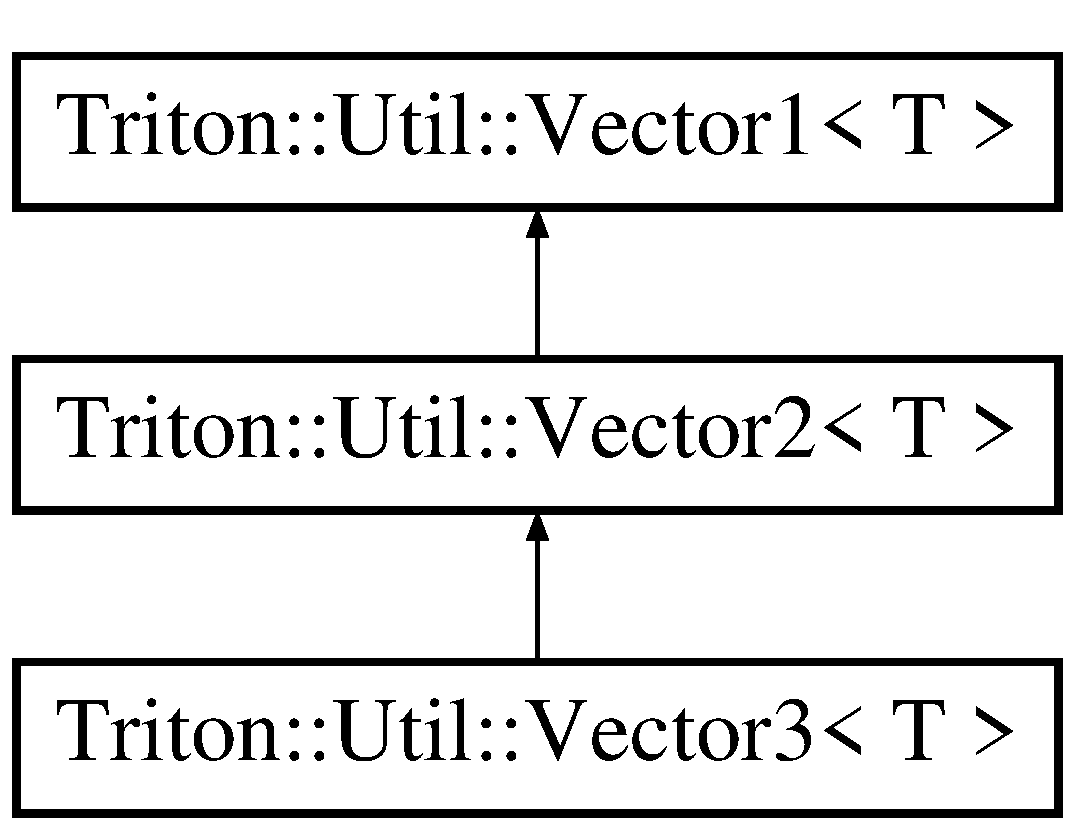
\includegraphics[height=3.000000cm]{class_triton_1_1_util_1_1_vector2}
\end{center}
\end{figure}
\subsection*{Public Member Functions}
\begin{DoxyCompactItemize}
\item 
\hyperlink{class_triton_1_1_util_1_1_vector2_a2b54901725ae54bd42f40c710ae976d9}{Vector2} (T X=0, T Y=0)
\begin{DoxyCompactList}\small\item\em Construct the vector from its coordinates. \end{DoxyCompactList}\item 
{\footnotesize template$<$typename U $>$ }\\\hyperlink{class_triton_1_1_util_1_1_vector2_ae06128c7bf34f56168c91555a10a638d}{Vector2} (const \hyperlink{class_triton_1_1_util_1_1_vector1}{Vector1}$<$ U $>$ \&vector, T Y=0)
\begin{DoxyCompactList}\small\item\em Construct the vector from a \hyperlink{class_triton_1_1_util_1_1_vector1}{Triton\+::\+Util\+::\+Vector1} and a Z coordinate. \end{DoxyCompactList}\item 
{\footnotesize template$<$typename U $>$ }\\\hyperlink{class_triton_1_1_util_1_1_vector2}{Vector2}$<$ T $>$ \& \hyperlink{class_triton_1_1_util_1_1_vector2_a00b543ed959c5417e277e159dd0d0335}{operator=} (const \hyperlink{class_triton_1_1_util_1_1_vector1}{Vector1}$<$ U $>$ \&vector, T Y=0)
\begin{DoxyCompactList}\small\item\em An operator for evaluating \hyperlink{class_triton_1_1_util_1_1_vector1}{Triton\+::\+Util\+::\+Vector1} to a \hyperlink{class_triton_1_1_util_1_1_vector2}{Triton\+::\+Util\+::\+Vector2} using a Y coordinate parameter. \end{DoxyCompactList}\item 
{\footnotesize template$<$typename U $>$ }\\\hyperlink{class_triton_1_1_util_1_1_vector2}{Vector2}$<$ T $>$ \hyperlink{class_triton_1_1_util_1_1_vector2_a3acc6c063f70b0dcfe4994dc632e1ba6}{distance} (\hyperlink{class_triton_1_1_util_1_1_vector2}{Vector2}$<$ U $>$ vector)
\begin{DoxyCompactList}\small\item\em Returns a vector that holds the distance between this and vector. \end{DoxyCompactList}\item 
\hyperlink{class_triton_1_1_util_1_1_vector2}{Vector2}$<$ T $>$ \hyperlink{class_triton_1_1_util_1_1_vector2_a0a061ce609a249250a16c6dcfc84ac7e}{abs\+V2} ()
\begin{DoxyCompactList}\small\item\em Constructs a \hyperlink{class_triton_1_1_util_1_1_vector2}{Triton\+::\+Util\+::\+Vector2} with an absolute value of this vector. \end{DoxyCompactList}\end{DoxyCompactItemize}
\subsection*{Public Attributes}
\begin{DoxyCompactItemize}
\item 
T \hyperlink{class_triton_1_1_util_1_1_vector2_ae31b6d61a6efc64df0962052a71097b3}{m\+\_\+\+Y\+Position}
\begin{DoxyCompactList}\small\item\em Y coordinate of the vector. \end{DoxyCompactList}\end{DoxyCompactItemize}
\subsection*{Related Functions}
(Note that these are not member functions.) \begin{DoxyCompactItemize}
\item 
{\footnotesize template$<$typename T $>$ }\\\hyperlink{class_triton_1_1_util_1_1_vector2}{Vector2}$<$ T $>$ \hyperlink{class_triton_1_1_util_1_1_vector2_a3e0f93634ae76fec7f94ca462c2f41a5}{operator-\/} (const \hyperlink{class_triton_1_1_util_1_1_vector2}{Vector2}$<$ T $>$ \&left)
\begin{DoxyCompactList}\small\item\em Overload of unary operator -\/. \end{DoxyCompactList}\item 
{\footnotesize template$<$typename T $>$ }\\\hyperlink{class_triton_1_1_util_1_1_vector2}{Vector2}$<$ T $>$ \& \hyperlink{class_triton_1_1_util_1_1_vector2_ad4b7a9d355d57790bfc7df0ade8bb628}{operator+=} (\hyperlink{class_triton_1_1_util_1_1_vector2}{Vector2}$<$ T $>$ \&left, const \hyperlink{class_triton_1_1_util_1_1_vector2}{Vector2}$<$ T $>$ \&right)
\begin{DoxyCompactList}\small\item\em Overload of binary operator +=. \end{DoxyCompactList}\item 
{\footnotesize template$<$typename T $>$ }\\\hyperlink{class_triton_1_1_util_1_1_vector2}{Vector2}$<$ T $>$ \& \hyperlink{class_triton_1_1_util_1_1_vector2_a30a5a12ad03c9a3a982a0a313bf84e6f}{operator-\/=} (\hyperlink{class_triton_1_1_util_1_1_vector2}{Vector2}$<$ T $>$ \&left, const \hyperlink{class_triton_1_1_util_1_1_vector2}{Vector2}$<$ T $>$ \&right)
\begin{DoxyCompactList}\small\item\em Overload of binary operator -\/=. \end{DoxyCompactList}\item 
{\footnotesize template$<$typename T $>$ }\\\hyperlink{class_triton_1_1_util_1_1_vector2}{Vector2}$<$ T $>$ \hyperlink{class_triton_1_1_util_1_1_vector2_a72421239823c38a6b780c86a710ead07}{operator+} (const \hyperlink{class_triton_1_1_util_1_1_vector2}{Vector2}$<$ T $>$ \&left, const \hyperlink{class_triton_1_1_util_1_1_vector2}{Vector2}$<$ T $>$ \&right)
\begin{DoxyCompactList}\small\item\em Overload of binary operator +. \end{DoxyCompactList}\item 
{\footnotesize template$<$typename T $>$ }\\\hyperlink{class_triton_1_1_util_1_1_vector2}{Vector2}$<$ T $>$ \hyperlink{class_triton_1_1_util_1_1_vector2_ad027adae53ec547a86c20deeb05c9e85}{operator-\/} (const \hyperlink{class_triton_1_1_util_1_1_vector2}{Vector2}$<$ T $>$ \&left, const \hyperlink{class_triton_1_1_util_1_1_vector2}{Vector2}$<$ T $>$ \&right)
\begin{DoxyCompactList}\small\item\em Overload of binary operator -\/. \end{DoxyCompactList}\item 
{\footnotesize template$<$typename T $>$ }\\\hyperlink{class_triton_1_1_util_1_1_vector2}{Vector2}$<$ T $>$ \hyperlink{class_triton_1_1_util_1_1_vector2_a5f48ca928995b41c89f155afe8d16b02}{operator$\ast$} (const \hyperlink{class_triton_1_1_util_1_1_vector2}{Vector2}$<$ T $>$ \&left, T right)
\begin{DoxyCompactList}\small\item\em Overload of binary operator $\ast$. \end{DoxyCompactList}\item 
{\footnotesize template$<$typename T $>$ }\\\hyperlink{class_triton_1_1_util_1_1_vector2}{Vector2}$<$ T $>$ \hyperlink{class_triton_1_1_util_1_1_vector2_ad8b3e1cf7b156a984bc1427539ca8605}{operator$\ast$} (T left, const \hyperlink{class_triton_1_1_util_1_1_vector2}{Vector2}$<$ T $>$ \&right)
\begin{DoxyCompactList}\small\item\em Overload of binary operator $\ast$. \end{DoxyCompactList}\item 
{\footnotesize template$<$typename T $>$ }\\\hyperlink{class_triton_1_1_util_1_1_vector2}{Vector2}$<$ T $>$ \& \hyperlink{class_triton_1_1_util_1_1_vector2_abea24cb28c0d6e2957e259ba4e65d70e}{operator$\ast$=} (\hyperlink{class_triton_1_1_util_1_1_vector2}{Vector2}$<$ T $>$ \&left, T right)
\begin{DoxyCompactList}\small\item\em Overload of binary operator $\ast$=. \end{DoxyCompactList}\item 
{\footnotesize template$<$typename T $>$ }\\\hyperlink{class_triton_1_1_util_1_1_vector2}{Vector2}$<$ T $>$ \hyperlink{class_triton_1_1_util_1_1_vector2_a7409dd89cb3aad6c3bc6622311107311}{operator/} (const \hyperlink{class_triton_1_1_util_1_1_vector2}{Vector2}$<$ T $>$ \&left, T right)
\begin{DoxyCompactList}\small\item\em Overload of binary operator /. \end{DoxyCompactList}\item 
{\footnotesize template$<$typename T $>$ }\\\hyperlink{class_triton_1_1_util_1_1_vector2}{Vector2}$<$ T $>$ \& \hyperlink{class_triton_1_1_util_1_1_vector2_ac4d293c9dc7954ccfd5e373972f38b03}{operator/=} (\hyperlink{class_triton_1_1_util_1_1_vector2}{Vector2}$<$ T $>$ \&left, T right)
\begin{DoxyCompactList}\small\item\em Overload of binary operator /=. \end{DoxyCompactList}\item 
{\footnotesize template$<$typename T $>$ }\\bool \hyperlink{class_triton_1_1_util_1_1_vector2_a9a7b2d36c3850828fdb651facfd25136}{operator==} (const \hyperlink{class_triton_1_1_util_1_1_vector2}{Vector2}$<$ T $>$ \&left, const \hyperlink{class_triton_1_1_util_1_1_vector2}{Vector2}$<$ T $>$ \&right)
\begin{DoxyCompactList}\small\item\em Overload of binary operator ==. \end{DoxyCompactList}\item 
{\footnotesize template$<$typename T $>$ }\\bool \hyperlink{class_triton_1_1_util_1_1_vector2_a01673da35ef9c52d0e54b8263549a956}{operator!=} (const \hyperlink{class_triton_1_1_util_1_1_vector2}{Vector2}$<$ T $>$ \&left, const \hyperlink{class_triton_1_1_util_1_1_vector2}{Vector2}$<$ T $>$ \&right)
\begin{DoxyCompactList}\small\item\em Overload of binary operator !=. \end{DoxyCompactList}\end{DoxyCompactItemize}


\subsection{Detailed Description}
\subsubsection*{template$<$typename T = int$>$class Triton\+::\+Util\+::\+Vector2$<$ T $>$}

Utility template class to store and manipulate 2-\/dimensional vector positions. 

Definition at line 17 of file Vector2.\+hpp.



\subsection{Constructor \& Destructor Documentation}
\hypertarget{class_triton_1_1_util_1_1_vector2_a2b54901725ae54bd42f40c710ae976d9}{}\index{Triton\+::\+Util\+::\+Vector2@{Triton\+::\+Util\+::\+Vector2}!Vector2@{Vector2}}
\index{Vector2@{Vector2}!Triton\+::\+Util\+::\+Vector2@{Triton\+::\+Util\+::\+Vector2}}
\subsubsection[{Vector2}]{\setlength{\rightskip}{0pt plus 5cm}template$<$typename T = int$>$ {\bf Triton\+::\+Util\+::\+Vector2}$<$ T $>$\+::{\bf Vector2} (
\begin{DoxyParamCaption}
\item[{T}]{X = {\ttfamily 0}, }
\item[{T}]{Y = {\ttfamily 0}}
\end{DoxyParamCaption}
)}\label{class_triton_1_1_util_1_1_vector2_a2b54901725ae54bd42f40c710ae976d9}


Construct the vector from its coordinates. 


\begin{DoxyParams}{Parameters}
{\em X} & X coordinate \\
\hline
{\em Y} & Y coordinate \\
\hline
\end{DoxyParams}
\hypertarget{class_triton_1_1_util_1_1_vector2_ae06128c7bf34f56168c91555a10a638d}{}\index{Triton\+::\+Util\+::\+Vector2@{Triton\+::\+Util\+::\+Vector2}!Vector2@{Vector2}}
\index{Vector2@{Vector2}!Triton\+::\+Util\+::\+Vector2@{Triton\+::\+Util\+::\+Vector2}}
\subsubsection[{Vector2}]{\setlength{\rightskip}{0pt plus 5cm}template$<$typename T = int$>$ template$<$typename U $>$ {\bf Triton\+::\+Util\+::\+Vector2}$<$ T $>$\+::{\bf Vector2} (
\begin{DoxyParamCaption}
\item[{const {\bf Vector1}$<$ U $>$ \&}]{vector, }
\item[{T}]{Y = {\ttfamily 0}}
\end{DoxyParamCaption}
)}\label{class_triton_1_1_util_1_1_vector2_ae06128c7bf34f56168c91555a10a638d}


Construct the vector from a \hyperlink{class_triton_1_1_util_1_1_vector1}{Triton\+::\+Util\+::\+Vector1} and a Z coordinate. 


\begin{DoxyExceptions}{Exceptions}
{\em Exception\+Cast\+Fail} & thrown when U can\textquotesingle{}t be casted to T\\
\hline
\end{DoxyExceptions}

\begin{DoxyParams}{Parameters}
{\em vector} & Vector to convert \\
\hline
{\em Y} & the new Y coordinate \\
\hline
\end{DoxyParams}


\subsection{Member Function Documentation}
\hypertarget{class_triton_1_1_util_1_1_vector2_a0a061ce609a249250a16c6dcfc84ac7e}{}\index{Triton\+::\+Util\+::\+Vector2@{Triton\+::\+Util\+::\+Vector2}!abs\+V2@{abs\+V2}}
\index{abs\+V2@{abs\+V2}!Triton\+::\+Util\+::\+Vector2@{Triton\+::\+Util\+::\+Vector2}}
\subsubsection[{abs\+V2}]{\setlength{\rightskip}{0pt plus 5cm}template$<$typename T = int$>$ {\bf Vector2}$<$T$>$ {\bf Triton\+::\+Util\+::\+Vector2}$<$ T $>$\+::abs\+V2 (
\begin{DoxyParamCaption}
{}
\end{DoxyParamCaption}
)}\label{class_triton_1_1_util_1_1_vector2_a0a061ce609a249250a16c6dcfc84ac7e}


Constructs a \hyperlink{class_triton_1_1_util_1_1_vector2}{Triton\+::\+Util\+::\+Vector2} with an absolute value of this vector. 

\hypertarget{class_triton_1_1_util_1_1_vector2_a3acc6c063f70b0dcfe4994dc632e1ba6}{}\index{Triton\+::\+Util\+::\+Vector2@{Triton\+::\+Util\+::\+Vector2}!distance@{distance}}
\index{distance@{distance}!Triton\+::\+Util\+::\+Vector2@{Triton\+::\+Util\+::\+Vector2}}
\subsubsection[{distance}]{\setlength{\rightskip}{0pt plus 5cm}template$<$typename T = int$>$ template$<$typename U $>$ {\bf Vector2}$<$T$>$ {\bf Triton\+::\+Util\+::\+Vector2}$<$ T $>$\+::distance (
\begin{DoxyParamCaption}
\item[{{\bf Vector2}$<$ U $>$}]{vector}
\end{DoxyParamCaption}
)}\label{class_triton_1_1_util_1_1_vector2_a3acc6c063f70b0dcfe4994dc632e1ba6}


Returns a vector that holds the distance between this and vector. 

\begin{DoxyNote}{Note}
The distance is an absolute value
\end{DoxyNote}

\begin{DoxyExceptions}{Exceptions}
{\em Exception\+Cast\+Fail} & thrown when U can\textquotesingle{}t be casted to T\\
\hline
\end{DoxyExceptions}

\begin{DoxyParams}{Parameters}
{\em vector} & Vector to other vector \\
\hline
\end{DoxyParams}
\hypertarget{class_triton_1_1_util_1_1_vector2_a00b543ed959c5417e277e159dd0d0335}{}\index{Triton\+::\+Util\+::\+Vector2@{Triton\+::\+Util\+::\+Vector2}!operator=@{operator=}}
\index{operator=@{operator=}!Triton\+::\+Util\+::\+Vector2@{Triton\+::\+Util\+::\+Vector2}}
\subsubsection[{operator=}]{\setlength{\rightskip}{0pt plus 5cm}template$<$typename T = int$>$ template$<$typename U $>$ {\bf Vector2}$<$T$>$\& {\bf Triton\+::\+Util\+::\+Vector2}$<$ T $>$\+::operator= (
\begin{DoxyParamCaption}
\item[{const {\bf Vector1}$<$ U $>$ \&}]{vector, }
\item[{T}]{Y = {\ttfamily 0}}
\end{DoxyParamCaption}
)}\label{class_triton_1_1_util_1_1_vector2_a00b543ed959c5417e277e159dd0d0335}


An operator for evaluating \hyperlink{class_triton_1_1_util_1_1_vector1}{Triton\+::\+Util\+::\+Vector1} to a \hyperlink{class_triton_1_1_util_1_1_vector2}{Triton\+::\+Util\+::\+Vector2} using a Y coordinate parameter. 


\begin{DoxyExceptions}{Exceptions}
{\em Exception\+Cast\+Fail} & thrown when U can\textquotesingle{}t be casted to T\\
\hline
\end{DoxyExceptions}

\begin{DoxyParams}{Parameters}
{\em vector} & Vector to convert \\
\hline
{\em Y} & the new Y coordinate \\
\hline
\end{DoxyParams}


\subsection{Friends And Related Function Documentation}
\hypertarget{class_triton_1_1_util_1_1_vector2_a01673da35ef9c52d0e54b8263549a956}{}\index{Triton\+::\+Util\+::\+Vector2@{Triton\+::\+Util\+::\+Vector2}!operator"!=@{operator"!=}}
\index{operator"!=@{operator"!=}!Triton\+::\+Util\+::\+Vector2@{Triton\+::\+Util\+::\+Vector2}}
\subsubsection[{operator"!=}]{\setlength{\rightskip}{0pt plus 5cm}template$<$typename T $>$ bool operator!= (
\begin{DoxyParamCaption}
\item[{const {\bf Vector2}$<$ T $>$ \&}]{left, }
\item[{const {\bf Vector2}$<$ T $>$ \&}]{right}
\end{DoxyParamCaption}
)\hspace{0.3cm}{\ttfamily [related]}}\label{class_triton_1_1_util_1_1_vector2_a01673da35ef9c52d0e54b8263549a956}


Overload of binary operator !=. 

This operator compares strict difference between two vectors.


\begin{DoxyParams}{Parameters}
{\em left} & Left operand (a vector) \\
\hline
{\em right} & Right operand (a vector)\\
\hline
\end{DoxyParams}
\begin{DoxyReturn}{Returns}
True if {\itshape left} is not equal to {\itshape right} 
\end{DoxyReturn}
\hypertarget{class_triton_1_1_util_1_1_vector2_a5f48ca928995b41c89f155afe8d16b02}{}\index{Triton\+::\+Util\+::\+Vector2@{Triton\+::\+Util\+::\+Vector2}!operator$\ast$@{operator$\ast$}}
\index{operator$\ast$@{operator$\ast$}!Triton\+::\+Util\+::\+Vector2@{Triton\+::\+Util\+::\+Vector2}}
\subsubsection[{operator$\ast$}]{\setlength{\rightskip}{0pt plus 5cm}template$<$typename T $>$ {\bf Vector2}$<$ T $>$ operator$\ast$ (
\begin{DoxyParamCaption}
\item[{const {\bf Vector2}$<$ T $>$ \&}]{left, }
\item[{T}]{right}
\end{DoxyParamCaption}
)\hspace{0.3cm}{\ttfamily [related]}}\label{class_triton_1_1_util_1_1_vector2_a5f48ca928995b41c89f155afe8d16b02}


Overload of binary operator $\ast$. 


\begin{DoxyParams}{Parameters}
{\em left} & Left operand (a vector) \\
\hline
{\em right} & Right operand (a scalar value)\\
\hline
\end{DoxyParams}
\begin{DoxyReturn}{Returns}
Memberwise multiplication by {\itshape right} 
\end{DoxyReturn}
\hypertarget{class_triton_1_1_util_1_1_vector2_ad8b3e1cf7b156a984bc1427539ca8605}{}\index{Triton\+::\+Util\+::\+Vector2@{Triton\+::\+Util\+::\+Vector2}!operator$\ast$@{operator$\ast$}}
\index{operator$\ast$@{operator$\ast$}!Triton\+::\+Util\+::\+Vector2@{Triton\+::\+Util\+::\+Vector2}}
\subsubsection[{operator$\ast$}]{\setlength{\rightskip}{0pt plus 5cm}template$<$typename T $>$ {\bf Vector2}$<$ T $>$ operator$\ast$ (
\begin{DoxyParamCaption}
\item[{T}]{left, }
\item[{const {\bf Vector2}$<$ T $>$ \&}]{right}
\end{DoxyParamCaption}
)\hspace{0.3cm}{\ttfamily [related]}}\label{class_triton_1_1_util_1_1_vector2_ad8b3e1cf7b156a984bc1427539ca8605}


Overload of binary operator $\ast$. 


\begin{DoxyParams}{Parameters}
{\em left} & Left operand (a scalar value) \\
\hline
{\em right} & Right operand (a vector)\\
\hline
\end{DoxyParams}
\begin{DoxyReturn}{Returns}
Memberwise multiplication by {\itshape left} 
\end{DoxyReturn}
\hypertarget{class_triton_1_1_util_1_1_vector2_abea24cb28c0d6e2957e259ba4e65d70e}{}\index{Triton\+::\+Util\+::\+Vector2@{Triton\+::\+Util\+::\+Vector2}!operator$\ast$=@{operator$\ast$=}}
\index{operator$\ast$=@{operator$\ast$=}!Triton\+::\+Util\+::\+Vector2@{Triton\+::\+Util\+::\+Vector2}}
\subsubsection[{operator$\ast$=}]{\setlength{\rightskip}{0pt plus 5cm}template$<$typename T $>$ {\bf Vector2}$<$ T $>$ \& operator$\ast$= (
\begin{DoxyParamCaption}
\item[{{\bf Vector2}$<$ T $>$ \&}]{left, }
\item[{T}]{right}
\end{DoxyParamCaption}
)\hspace{0.3cm}{\ttfamily [related]}}\label{class_triton_1_1_util_1_1_vector2_abea24cb28c0d6e2957e259ba4e65d70e}


Overload of binary operator $\ast$=. 

This operator performs a memberwise multiplication by {\itshape right}, and assigns the result to {\itshape left}.


\begin{DoxyParams}{Parameters}
{\em left} & Left operand (a vector) \\
\hline
{\em right} & Right operand (a scalar value)\\
\hline
\end{DoxyParams}
\begin{DoxyReturn}{Returns}
Reference to {\itshape left} 
\end{DoxyReturn}
\hypertarget{class_triton_1_1_util_1_1_vector2_a72421239823c38a6b780c86a710ead07}{}\index{Triton\+::\+Util\+::\+Vector2@{Triton\+::\+Util\+::\+Vector2}!operator+@{operator+}}
\index{operator+@{operator+}!Triton\+::\+Util\+::\+Vector2@{Triton\+::\+Util\+::\+Vector2}}
\subsubsection[{operator+}]{\setlength{\rightskip}{0pt plus 5cm}template$<$typename T $>$ {\bf Vector2}$<$ T $>$ operator+ (
\begin{DoxyParamCaption}
\item[{const {\bf Vector2}$<$ T $>$ \&}]{left, }
\item[{const {\bf Vector2}$<$ T $>$ \&}]{right}
\end{DoxyParamCaption}
)\hspace{0.3cm}{\ttfamily [related]}}\label{class_triton_1_1_util_1_1_vector2_a72421239823c38a6b780c86a710ead07}


Overload of binary operator +. 


\begin{DoxyParams}{Parameters}
{\em left} & Left operand (a vector) \\
\hline
{\em right} & Right operand (a vector)\\
\hline
\end{DoxyParams}
\begin{DoxyReturn}{Returns}
Memberwise addition of both vectors 
\end{DoxyReturn}
\hypertarget{class_triton_1_1_util_1_1_vector2_ad4b7a9d355d57790bfc7df0ade8bb628}{}\index{Triton\+::\+Util\+::\+Vector2@{Triton\+::\+Util\+::\+Vector2}!operator+=@{operator+=}}
\index{operator+=@{operator+=}!Triton\+::\+Util\+::\+Vector2@{Triton\+::\+Util\+::\+Vector2}}
\subsubsection[{operator+=}]{\setlength{\rightskip}{0pt plus 5cm}template$<$typename T $>$ {\bf Vector2}$<$ T $>$ \& operator+= (
\begin{DoxyParamCaption}
\item[{{\bf Vector2}$<$ T $>$ \&}]{left, }
\item[{const {\bf Vector2}$<$ T $>$ \&}]{right}
\end{DoxyParamCaption}
)\hspace{0.3cm}{\ttfamily [related]}}\label{class_triton_1_1_util_1_1_vector2_ad4b7a9d355d57790bfc7df0ade8bb628}


Overload of binary operator +=. 

This operator performs a memberwise addition of both vectors, and assigns the result to {\itshape left}.


\begin{DoxyParams}{Parameters}
{\em left} & Left operand (a vector) \\
\hline
{\em right} & Right operand (a vector)\\
\hline
\end{DoxyParams}
\begin{DoxyReturn}{Returns}
Reference to {\itshape left} 
\end{DoxyReturn}
\hypertarget{class_triton_1_1_util_1_1_vector2_a3e0f93634ae76fec7f94ca462c2f41a5}{}\index{Triton\+::\+Util\+::\+Vector2@{Triton\+::\+Util\+::\+Vector2}!operator-\/@{operator-\/}}
\index{operator-\/@{operator-\/}!Triton\+::\+Util\+::\+Vector2@{Triton\+::\+Util\+::\+Vector2}}
\subsubsection[{operator-\/}]{\setlength{\rightskip}{0pt plus 5cm}template$<$typename T $>$ {\bf Vector2}$<$ T $>$ operator-\/ (
\begin{DoxyParamCaption}
\item[{const {\bf Vector2}$<$ T $>$ \&}]{left}
\end{DoxyParamCaption}
)\hspace{0.3cm}{\ttfamily [related]}}\label{class_triton_1_1_util_1_1_vector2_a3e0f93634ae76fec7f94ca462c2f41a5}


Overload of unary operator -\/. 


\begin{DoxyParams}{Parameters}
{\em left} & Vector to negate\\
\hline
\end{DoxyParams}
\begin{DoxyReturn}{Returns}
Memberwise opposite of the vector 
\end{DoxyReturn}
\hypertarget{class_triton_1_1_util_1_1_vector2_ad027adae53ec547a86c20deeb05c9e85}{}\index{Triton\+::\+Util\+::\+Vector2@{Triton\+::\+Util\+::\+Vector2}!operator-\/@{operator-\/}}
\index{operator-\/@{operator-\/}!Triton\+::\+Util\+::\+Vector2@{Triton\+::\+Util\+::\+Vector2}}
\subsubsection[{operator-\/}]{\setlength{\rightskip}{0pt plus 5cm}template$<$typename T $>$ {\bf Vector2}$<$ T $>$ operator-\/ (
\begin{DoxyParamCaption}
\item[{const {\bf Vector2}$<$ T $>$ \&}]{left, }
\item[{const {\bf Vector2}$<$ T $>$ \&}]{right}
\end{DoxyParamCaption}
)\hspace{0.3cm}{\ttfamily [related]}}\label{class_triton_1_1_util_1_1_vector2_ad027adae53ec547a86c20deeb05c9e85}


Overload of binary operator -\/. 


\begin{DoxyParams}{Parameters}
{\em left} & Left operand (a vector) \\
\hline
{\em right} & Right operand (a vector)\\
\hline
\end{DoxyParams}
\begin{DoxyReturn}{Returns}
Memberwise subtraction of both vectors 
\end{DoxyReturn}
\hypertarget{class_triton_1_1_util_1_1_vector2_a30a5a12ad03c9a3a982a0a313bf84e6f}{}\index{Triton\+::\+Util\+::\+Vector2@{Triton\+::\+Util\+::\+Vector2}!operator-\/=@{operator-\/=}}
\index{operator-\/=@{operator-\/=}!Triton\+::\+Util\+::\+Vector2@{Triton\+::\+Util\+::\+Vector2}}
\subsubsection[{operator-\/=}]{\setlength{\rightskip}{0pt plus 5cm}template$<$typename T $>$ {\bf Vector2}$<$ T $>$ \& operator-\/= (
\begin{DoxyParamCaption}
\item[{{\bf Vector2}$<$ T $>$ \&}]{left, }
\item[{const {\bf Vector2}$<$ T $>$ \&}]{right}
\end{DoxyParamCaption}
)\hspace{0.3cm}{\ttfamily [related]}}\label{class_triton_1_1_util_1_1_vector2_a30a5a12ad03c9a3a982a0a313bf84e6f}


Overload of binary operator -\/=. 

This operator performs a memberwise subtraction of both vectors, and assigns the result to {\itshape left}.


\begin{DoxyParams}{Parameters}
{\em left} & Left operand (a vector) \\
\hline
{\em right} & Right operand (a vector)\\
\hline
\end{DoxyParams}
\begin{DoxyReturn}{Returns}
Reference to {\itshape left} 
\end{DoxyReturn}
\hypertarget{class_triton_1_1_util_1_1_vector2_a7409dd89cb3aad6c3bc6622311107311}{}\index{Triton\+::\+Util\+::\+Vector2@{Triton\+::\+Util\+::\+Vector2}!operator/@{operator/}}
\index{operator/@{operator/}!Triton\+::\+Util\+::\+Vector2@{Triton\+::\+Util\+::\+Vector2}}
\subsubsection[{operator/}]{\setlength{\rightskip}{0pt plus 5cm}template$<$typename T $>$ {\bf Vector2}$<$ T $>$ operator/ (
\begin{DoxyParamCaption}
\item[{const {\bf Vector2}$<$ T $>$ \&}]{left, }
\item[{T}]{right}
\end{DoxyParamCaption}
)\hspace{0.3cm}{\ttfamily [related]}}\label{class_triton_1_1_util_1_1_vector2_a7409dd89cb3aad6c3bc6622311107311}


Overload of binary operator /. 


\begin{DoxyParams}{Parameters}
{\em left} & Left operand (a vector) \\
\hline
{\em right} & Right operand (a scalar value)\\
\hline
\end{DoxyParams}
\begin{DoxyReturn}{Returns}
Memberwise division by {\itshape right} 
\end{DoxyReturn}
\hypertarget{class_triton_1_1_util_1_1_vector2_ac4d293c9dc7954ccfd5e373972f38b03}{}\index{Triton\+::\+Util\+::\+Vector2@{Triton\+::\+Util\+::\+Vector2}!operator/=@{operator/=}}
\index{operator/=@{operator/=}!Triton\+::\+Util\+::\+Vector2@{Triton\+::\+Util\+::\+Vector2}}
\subsubsection[{operator/=}]{\setlength{\rightskip}{0pt plus 5cm}template$<$typename T $>$ {\bf Vector2}$<$ T $>$ \& operator/= (
\begin{DoxyParamCaption}
\item[{{\bf Vector2}$<$ T $>$ \&}]{left, }
\item[{T}]{right}
\end{DoxyParamCaption}
)\hspace{0.3cm}{\ttfamily [related]}}\label{class_triton_1_1_util_1_1_vector2_ac4d293c9dc7954ccfd5e373972f38b03}


Overload of binary operator /=. 

This operator performs a memberwise division by {\itshape right}, and assigns the result to {\itshape left}.


\begin{DoxyParams}{Parameters}
{\em left} & Left operand (a vector) \\
\hline
{\em right} & Right operand (a scalar value)\\
\hline
\end{DoxyParams}
\begin{DoxyReturn}{Returns}
Reference to {\itshape left} 
\end{DoxyReturn}
\hypertarget{class_triton_1_1_util_1_1_vector2_a9a7b2d36c3850828fdb651facfd25136}{}\index{Triton\+::\+Util\+::\+Vector2@{Triton\+::\+Util\+::\+Vector2}!operator==@{operator==}}
\index{operator==@{operator==}!Triton\+::\+Util\+::\+Vector2@{Triton\+::\+Util\+::\+Vector2}}
\subsubsection[{operator==}]{\setlength{\rightskip}{0pt plus 5cm}template$<$typename T $>$ bool operator== (
\begin{DoxyParamCaption}
\item[{const {\bf Vector2}$<$ T $>$ \&}]{left, }
\item[{const {\bf Vector2}$<$ T $>$ \&}]{right}
\end{DoxyParamCaption}
)\hspace{0.3cm}{\ttfamily [related]}}\label{class_triton_1_1_util_1_1_vector2_a9a7b2d36c3850828fdb651facfd25136}


Overload of binary operator ==. 

This operator compares strict equality between two vectors.


\begin{DoxyParams}{Parameters}
{\em left} & Left operand (a vector) \\
\hline
{\em right} & Right operand (a vector)\\
\hline
\end{DoxyParams}
\begin{DoxyReturn}{Returns}
True if {\itshape left} is equal to {\itshape right} 
\end{DoxyReturn}


\subsection{Member Data Documentation}
\hypertarget{class_triton_1_1_util_1_1_vector2_ae31b6d61a6efc64df0962052a71097b3}{}\index{Triton\+::\+Util\+::\+Vector2@{Triton\+::\+Util\+::\+Vector2}!m\+\_\+\+Y\+Position@{m\+\_\+\+Y\+Position}}
\index{m\+\_\+\+Y\+Position@{m\+\_\+\+Y\+Position}!Triton\+::\+Util\+::\+Vector2@{Triton\+::\+Util\+::\+Vector2}}
\subsubsection[{m\+\_\+\+Y\+Position}]{\setlength{\rightskip}{0pt plus 5cm}template$<$typename T = int$>$ T {\bf Triton\+::\+Util\+::\+Vector2}$<$ T $>$\+::m\+\_\+\+Y\+Position}\label{class_triton_1_1_util_1_1_vector2_ae31b6d61a6efc64df0962052a71097b3}


Y coordinate of the vector. 



Definition at line 85 of file Vector2.\+hpp.



The documentation for this class was generated from the following file\+:\begin{DoxyCompactItemize}
\item 
util/\hyperlink{_vector2_8hpp}{Vector2.\+hpp}\end{DoxyCompactItemize}

\hypertarget{class_triton_1_1_util_1_1_vector3}{}\section{Triton\+:\+:Util\+:\+:Vector3$<$ T $>$ Class Template Reference}
\label{class_triton_1_1_util_1_1_vector3}\index{Triton\+::\+Util\+::\+Vector3$<$ T $>$@{Triton\+::\+Util\+::\+Vector3$<$ T $>$}}


Utility template class to store and manipulate 3-\/dimensional vector positions.  




{\ttfamily \#include $<$Vector3.\+hpp$>$}

Inheritance diagram for Triton\+:\+:Util\+:\+:Vector3$<$ T $>$\+:\begin{figure}[H]
\begin{center}
\leavevmode
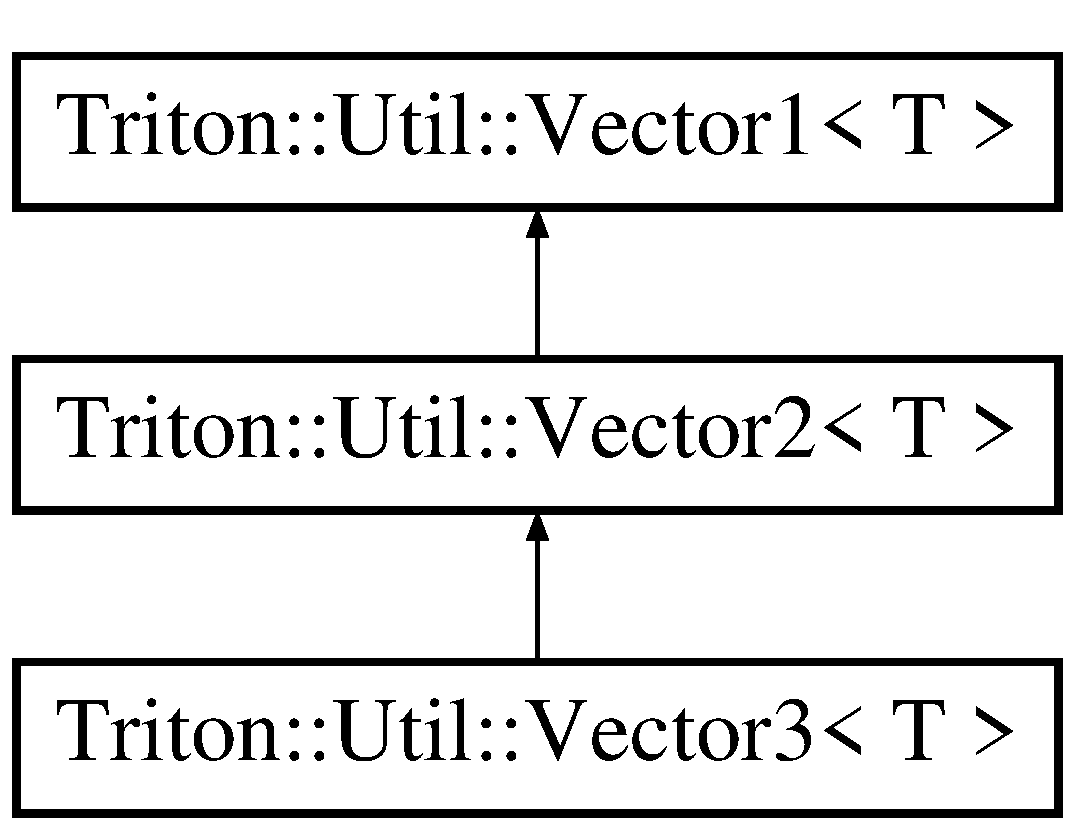
\includegraphics[height=3.000000cm]{class_triton_1_1_util_1_1_vector3}
\end{center}
\end{figure}
\subsection*{Public Member Functions}
\begin{DoxyCompactItemize}
\item 
\hyperlink{class_triton_1_1_util_1_1_vector3_a7ff2d48cbf361a1c29dcfa7922cc7f76}{Vector3} (T X=0, T Y=0, T Z=0)
\begin{DoxyCompactList}\small\item\em Construct the vector from its coordinates, also treated as default constructor. \end{DoxyCompactList}\item 
{\footnotesize template$<$typename U $>$ }\\\hyperlink{class_triton_1_1_util_1_1_vector3_a38db25895019ecbfd2f4bfb7af4ea569}{Vector3} (const \hyperlink{class_triton_1_1_util_1_1_vector1}{Vector1}$<$ U $>$ \&vector, T Y=0, T Z=0)
\begin{DoxyCompactList}\small\item\em Construct the vector from a \hyperlink{class_triton_1_1_util_1_1_vector1}{Triton\+::\+Util\+::\+Vector1}, a Y coordinate, and Z coordinate. \end{DoxyCompactList}\item 
{\footnotesize template$<$typename U $>$ }\\\hyperlink{class_triton_1_1_util_1_1_vector3_ad4d789aa3a7b5974230b7c4c6018d1f1}{Vector3} (const \hyperlink{class_triton_1_1_util_1_1_vector2}{Vector2}$<$ U $>$ \&vector, T Z=0)
\begin{DoxyCompactList}\small\item\em Construct the vector from a \hyperlink{class_triton_1_1_util_1_1_vector2}{Triton\+::\+Util\+::\+Vector2} and a Z coordinate. \end{DoxyCompactList}\item 
{\footnotesize template$<$typename U $>$ }\\\hyperlink{class_triton_1_1_util_1_1_vector3}{Vector3}$<$ T $>$ \& \hyperlink{class_triton_1_1_util_1_1_vector3_a73fccfb26f18c94bb62e33de03ecf9c1}{operator=} (const \hyperlink{class_triton_1_1_util_1_1_vector1}{Vector1}$<$ U $>$ \&vector, T Y=0, T Z=0)
\begin{DoxyCompactList}\small\item\em An operator for evaluating \hyperlink{class_triton_1_1_util_1_1_vector1}{Triton\+::\+Util\+::\+Vector1} to a \hyperlink{class_triton_1_1_util_1_1_vector3}{Triton\+::\+Util\+::\+Vector3} using Y and Z coordinate parameters. \end{DoxyCompactList}\item 
{\footnotesize template$<$typename U $>$ }\\\hyperlink{class_triton_1_1_util_1_1_vector3}{Vector3}$<$ T $>$ \& \hyperlink{class_triton_1_1_util_1_1_vector3_ac27ac77c9ed4cca294ae21a51fa1cdfc}{operator=} (const \hyperlink{class_triton_1_1_util_1_1_vector2}{Vector2}$<$ U $>$ \&vector, T Z=0)
\begin{DoxyCompactList}\small\item\em An operator for evaluating \hyperlink{class_triton_1_1_util_1_1_vector2}{Triton\+::\+Util\+::\+Vector2} to a \hyperlink{class_triton_1_1_util_1_1_vector3}{Triton\+::\+Util\+::\+Vector3} using a Z coordinate parameter. \end{DoxyCompactList}\item 
{\footnotesize template$<$typename U $>$ }\\\hyperlink{class_triton_1_1_util_1_1_vector3}{Vector3}$<$ T $>$ \hyperlink{class_triton_1_1_util_1_1_vector3_a00f99640d34d3c596c5c665384249c3e}{distance} (\hyperlink{class_triton_1_1_util_1_1_vector3}{Vector3}$<$ U $>$ vector)
\begin{DoxyCompactList}\small\item\em Returns a vector that holds the distance between this and vector. \end{DoxyCompactList}\item 
\hyperlink{class_triton_1_1_util_1_1_vector3}{Vector3}$<$ T $>$ \hyperlink{class_triton_1_1_util_1_1_vector3_a3b86bff74414a8de65ce908a9e4a686f}{abs\+V3} ()
\begin{DoxyCompactList}\small\item\em Constructs a \hyperlink{class_triton_1_1_util_1_1_vector3}{Triton\+::\+Util\+::\+Vector3} with an absolute value of this vector. \end{DoxyCompactList}\end{DoxyCompactItemize}
\subsection*{Public Attributes}
\begin{DoxyCompactItemize}
\item 
T \hyperlink{class_triton_1_1_util_1_1_vector3_ac42aa6f29ac37a866b49cbc1d8e66f74}{m\+\_\+\+Z\+Position}
\begin{DoxyCompactList}\small\item\em Z coordinate of the vector. \end{DoxyCompactList}\end{DoxyCompactItemize}
\subsection*{Related Functions}
(Note that these are not member functions.) \begin{DoxyCompactItemize}
\item 
{\footnotesize template$<$typename T $>$ }\\\hyperlink{class_triton_1_1_util_1_1_vector3}{Vector3}$<$ T $>$ \hyperlink{class_triton_1_1_util_1_1_vector3_a9b75d2fb9b0f2fd9fe33f8f06f9dda75}{operator-\/} (const \hyperlink{class_triton_1_1_util_1_1_vector3}{Vector3}$<$ T $>$ \&left)
\begin{DoxyCompactList}\small\item\em Overload of unary operator -\/. \end{DoxyCompactList}\item 
{\footnotesize template$<$typename T $>$ }\\\hyperlink{class_triton_1_1_util_1_1_vector3}{Vector3}$<$ T $>$ \& \hyperlink{class_triton_1_1_util_1_1_vector3_abc28859af163c63318ea2723b81c5ad9}{operator+=} (\hyperlink{class_triton_1_1_util_1_1_vector3}{Vector3}$<$ T $>$ \&left, const \hyperlink{class_triton_1_1_util_1_1_vector3}{Vector3}$<$ T $>$ \&right)
\begin{DoxyCompactList}\small\item\em Overload of binary operator +=. \end{DoxyCompactList}\item 
{\footnotesize template$<$typename T $>$ }\\\hyperlink{class_triton_1_1_util_1_1_vector3}{Vector3}$<$ T $>$ \& \hyperlink{class_triton_1_1_util_1_1_vector3_aa465672d2a4ee5fd354e585cf08d2ab9}{operator-\/=} (\hyperlink{class_triton_1_1_util_1_1_vector3}{Vector3}$<$ T $>$ \&left, const \hyperlink{class_triton_1_1_util_1_1_vector3}{Vector3}$<$ T $>$ \&right)
\begin{DoxyCompactList}\small\item\em Overload of binary operator -\/=. \end{DoxyCompactList}\item 
{\footnotesize template$<$typename T $>$ }\\\hyperlink{class_triton_1_1_util_1_1_vector3}{Vector3}$<$ T $>$ \hyperlink{class_triton_1_1_util_1_1_vector3_a6500a0cb00e07801e9e9d7e96852ddd3}{operator+} (const \hyperlink{class_triton_1_1_util_1_1_vector3}{Vector3}$<$ T $>$ \&left, const \hyperlink{class_triton_1_1_util_1_1_vector3}{Vector3}$<$ T $>$ \&right)
\begin{DoxyCompactList}\small\item\em Overload of binary operator +. \end{DoxyCompactList}\item 
{\footnotesize template$<$typename T $>$ }\\\hyperlink{class_triton_1_1_util_1_1_vector3}{Vector3}$<$ T $>$ \hyperlink{class_triton_1_1_util_1_1_vector3_abe0b9411c00cf807bf8a5f835874bd2a}{operator-\/} (const \hyperlink{class_triton_1_1_util_1_1_vector3}{Vector3}$<$ T $>$ \&left, const \hyperlink{class_triton_1_1_util_1_1_vector3}{Vector3}$<$ T $>$ \&right)
\begin{DoxyCompactList}\small\item\em Overload of binary operator -\/. \end{DoxyCompactList}\item 
{\footnotesize template$<$typename T $>$ }\\\hyperlink{class_triton_1_1_util_1_1_vector3}{Vector3}$<$ T $>$ \hyperlink{class_triton_1_1_util_1_1_vector3_a44ec312b31c1a85dcff4863795f98329}{operator$\ast$} (const \hyperlink{class_triton_1_1_util_1_1_vector3}{Vector3}$<$ T $>$ \&left, T right)
\begin{DoxyCompactList}\small\item\em Overload of binary operator $\ast$. \end{DoxyCompactList}\item 
{\footnotesize template$<$typename T $>$ }\\\hyperlink{class_triton_1_1_util_1_1_vector3}{Vector3}$<$ T $>$ \hyperlink{class_triton_1_1_util_1_1_vector3_aa6f2b0d9f79c1b9774759b7087affbb1}{operator$\ast$} (T left, const \hyperlink{class_triton_1_1_util_1_1_vector3}{Vector3}$<$ T $>$ \&right)
\begin{DoxyCompactList}\small\item\em Overload of binary operator $\ast$. \end{DoxyCompactList}\item 
{\footnotesize template$<$typename T $>$ }\\\hyperlink{class_triton_1_1_util_1_1_vector3}{Vector3}$<$ T $>$ \& \hyperlink{class_triton_1_1_util_1_1_vector3_ad5fb972775ce8ab58cd9670789e806a7}{operator$\ast$=} (\hyperlink{class_triton_1_1_util_1_1_vector3}{Vector3}$<$ T $>$ \&left, T right)
\begin{DoxyCompactList}\small\item\em Overload of binary operator $\ast$=. \end{DoxyCompactList}\item 
{\footnotesize template$<$typename T $>$ }\\\hyperlink{class_triton_1_1_util_1_1_vector3}{Vector3}$<$ T $>$ \hyperlink{class_triton_1_1_util_1_1_vector3_ad4ba4a83de236ddeb92a7b759187e90d}{operator/} (const \hyperlink{class_triton_1_1_util_1_1_vector3}{Vector3}$<$ T $>$ \&left, T right)
\begin{DoxyCompactList}\small\item\em Overload of binary operator /. \end{DoxyCompactList}\item 
{\footnotesize template$<$typename T $>$ }\\\hyperlink{class_triton_1_1_util_1_1_vector3}{Vector3}$<$ T $>$ \& \hyperlink{class_triton_1_1_util_1_1_vector3_a8995a700f9dffccc6dddb3696ae17b64}{operator/=} (\hyperlink{class_triton_1_1_util_1_1_vector3}{Vector3}$<$ T $>$ \&left, T right)
\begin{DoxyCompactList}\small\item\em Overload of binary operator /=. \end{DoxyCompactList}\item 
{\footnotesize template$<$typename T $>$ }\\bool \hyperlink{class_triton_1_1_util_1_1_vector3_a388d72db973306a35ba467016b3dee30}{operator==} (const \hyperlink{class_triton_1_1_util_1_1_vector3}{Vector3}$<$ T $>$ \&left, const \hyperlink{class_triton_1_1_util_1_1_vector3}{Vector3}$<$ T $>$ \&right)
\begin{DoxyCompactList}\small\item\em Overload of binary operator ==. \end{DoxyCompactList}\item 
{\footnotesize template$<$typename T $>$ }\\bool \hyperlink{class_triton_1_1_util_1_1_vector3_a608500d1ad3b78082cb5bb4356742bd4}{operator!=} (const \hyperlink{class_triton_1_1_util_1_1_vector3}{Vector3}$<$ T $>$ \&left, const \hyperlink{class_triton_1_1_util_1_1_vector3}{Vector3}$<$ T $>$ \&right)
\begin{DoxyCompactList}\small\item\em Overload of binary operator !=. \end{DoxyCompactList}\end{DoxyCompactItemize}


\subsection{Detailed Description}
\subsubsection*{template$<$typename T = int$>$class Triton\+::\+Util\+::\+Vector3$<$ T $>$}

Utility template class to store and manipulate 3-\/dimensional vector positions. 

Definition at line 17 of file Vector3.\+hpp.



\subsection{Constructor \& Destructor Documentation}
\hypertarget{class_triton_1_1_util_1_1_vector3_a7ff2d48cbf361a1c29dcfa7922cc7f76}{}\index{Triton\+::\+Util\+::\+Vector3@{Triton\+::\+Util\+::\+Vector3}!Vector3@{Vector3}}
\index{Vector3@{Vector3}!Triton\+::\+Util\+::\+Vector3@{Triton\+::\+Util\+::\+Vector3}}
\subsubsection[{Vector3}]{\setlength{\rightskip}{0pt plus 5cm}template$<$typename T = int$>$ {\bf Triton\+::\+Util\+::\+Vector3}$<$ T $>$\+::{\bf Vector3} (
\begin{DoxyParamCaption}
\item[{T}]{X = {\ttfamily 0}, }
\item[{T}]{Y = {\ttfamily 0}, }
\item[{T}]{Z = {\ttfamily 0}}
\end{DoxyParamCaption}
)}\label{class_triton_1_1_util_1_1_vector3_a7ff2d48cbf361a1c29dcfa7922cc7f76}


Construct the vector from its coordinates, also treated as default constructor. 


\begin{DoxyParams}{Parameters}
{\em X} & X coordinate \\
\hline
{\em Y} & Y coordinate \\
\hline
{\em Z} & Z coordinate \\
\hline
\end{DoxyParams}
\hypertarget{class_triton_1_1_util_1_1_vector3_a38db25895019ecbfd2f4bfb7af4ea569}{}\index{Triton\+::\+Util\+::\+Vector3@{Triton\+::\+Util\+::\+Vector3}!Vector3@{Vector3}}
\index{Vector3@{Vector3}!Triton\+::\+Util\+::\+Vector3@{Triton\+::\+Util\+::\+Vector3}}
\subsubsection[{Vector3}]{\setlength{\rightskip}{0pt plus 5cm}template$<$typename T = int$>$ template$<$typename U $>$ {\bf Triton\+::\+Util\+::\+Vector3}$<$ T $>$\+::{\bf Vector3} (
\begin{DoxyParamCaption}
\item[{const {\bf Vector1}$<$ U $>$ \&}]{vector, }
\item[{T}]{Y = {\ttfamily 0}, }
\item[{T}]{Z = {\ttfamily 0}}
\end{DoxyParamCaption}
)}\label{class_triton_1_1_util_1_1_vector3_a38db25895019ecbfd2f4bfb7af4ea569}


Construct the vector from a \hyperlink{class_triton_1_1_util_1_1_vector1}{Triton\+::\+Util\+::\+Vector1}, a Y coordinate, and Z coordinate. 


\begin{DoxyExceptions}{Exceptions}
{\em Exception\+Cast\+Fail} & thrown when U can\textquotesingle{}t be casted to T\\
\hline
\end{DoxyExceptions}

\begin{DoxyParams}{Parameters}
{\em vector} & Vector to convert \\
\hline
{\em Y} & the new Y coordinate \\
\hline
{\em Z} & the new Z coordinate \\
\hline
\end{DoxyParams}
\hypertarget{class_triton_1_1_util_1_1_vector3_ad4d789aa3a7b5974230b7c4c6018d1f1}{}\index{Triton\+::\+Util\+::\+Vector3@{Triton\+::\+Util\+::\+Vector3}!Vector3@{Vector3}}
\index{Vector3@{Vector3}!Triton\+::\+Util\+::\+Vector3@{Triton\+::\+Util\+::\+Vector3}}
\subsubsection[{Vector3}]{\setlength{\rightskip}{0pt plus 5cm}template$<$typename T = int$>$ template$<$typename U $>$ {\bf Triton\+::\+Util\+::\+Vector3}$<$ T $>$\+::{\bf Vector3} (
\begin{DoxyParamCaption}
\item[{const {\bf Vector2}$<$ U $>$ \&}]{vector, }
\item[{T}]{Z = {\ttfamily 0}}
\end{DoxyParamCaption}
)}\label{class_triton_1_1_util_1_1_vector3_ad4d789aa3a7b5974230b7c4c6018d1f1}


Construct the vector from a \hyperlink{class_triton_1_1_util_1_1_vector2}{Triton\+::\+Util\+::\+Vector2} and a Z coordinate. 


\begin{DoxyExceptions}{Exceptions}
{\em Exception\+Cast\+Fail} & thrown when U can\textquotesingle{}t be casted to T\\
\hline
\end{DoxyExceptions}

\begin{DoxyParams}{Parameters}
{\em vector} & Vector to convert \\
\hline
{\em Z} & the new Z coordinate \\
\hline
\end{DoxyParams}


\subsection{Member Function Documentation}
\hypertarget{class_triton_1_1_util_1_1_vector3_a3b86bff74414a8de65ce908a9e4a686f}{}\index{Triton\+::\+Util\+::\+Vector3@{Triton\+::\+Util\+::\+Vector3}!abs\+V3@{abs\+V3}}
\index{abs\+V3@{abs\+V3}!Triton\+::\+Util\+::\+Vector3@{Triton\+::\+Util\+::\+Vector3}}
\subsubsection[{abs\+V3}]{\setlength{\rightskip}{0pt plus 5cm}template$<$typename T = int$>$ {\bf Vector3}$<$T$>$ {\bf Triton\+::\+Util\+::\+Vector3}$<$ T $>$\+::abs\+V3 (
\begin{DoxyParamCaption}
{}
\end{DoxyParamCaption}
)}\label{class_triton_1_1_util_1_1_vector3_a3b86bff74414a8de65ce908a9e4a686f}


Constructs a \hyperlink{class_triton_1_1_util_1_1_vector3}{Triton\+::\+Util\+::\+Vector3} with an absolute value of this vector. 

\hypertarget{class_triton_1_1_util_1_1_vector3_a00f99640d34d3c596c5c665384249c3e}{}\index{Triton\+::\+Util\+::\+Vector3@{Triton\+::\+Util\+::\+Vector3}!distance@{distance}}
\index{distance@{distance}!Triton\+::\+Util\+::\+Vector3@{Triton\+::\+Util\+::\+Vector3}}
\subsubsection[{distance}]{\setlength{\rightskip}{0pt plus 5cm}template$<$typename T = int$>$ template$<$typename U $>$ {\bf Vector3}$<$T$>$ {\bf Triton\+::\+Util\+::\+Vector3}$<$ T $>$\+::distance (
\begin{DoxyParamCaption}
\item[{{\bf Vector3}$<$ U $>$}]{vector}
\end{DoxyParamCaption}
)}\label{class_triton_1_1_util_1_1_vector3_a00f99640d34d3c596c5c665384249c3e}


Returns a vector that holds the distance between this and vector. 

\begin{DoxyNote}{Note}
The distance is an absolute value
\end{DoxyNote}

\begin{DoxyExceptions}{Exceptions}
{\em Exception\+Cast\+Fail} & thrown when U can\textquotesingle{}t be casted to T\\
\hline
\end{DoxyExceptions}

\begin{DoxyParams}{Parameters}
{\em vector} & Vector to other vector \\
\hline
\end{DoxyParams}
\hypertarget{class_triton_1_1_util_1_1_vector3_a73fccfb26f18c94bb62e33de03ecf9c1}{}\index{Triton\+::\+Util\+::\+Vector3@{Triton\+::\+Util\+::\+Vector3}!operator=@{operator=}}
\index{operator=@{operator=}!Triton\+::\+Util\+::\+Vector3@{Triton\+::\+Util\+::\+Vector3}}
\subsubsection[{operator=}]{\setlength{\rightskip}{0pt plus 5cm}template$<$typename T = int$>$ template$<$typename U $>$ {\bf Vector3}$<$T$>$\& {\bf Triton\+::\+Util\+::\+Vector3}$<$ T $>$\+::operator= (
\begin{DoxyParamCaption}
\item[{const {\bf Vector1}$<$ U $>$ \&}]{vector, }
\item[{T}]{Y = {\ttfamily 0}, }
\item[{T}]{Z = {\ttfamily 0}}
\end{DoxyParamCaption}
)}\label{class_triton_1_1_util_1_1_vector3_a73fccfb26f18c94bb62e33de03ecf9c1}


An operator for evaluating \hyperlink{class_triton_1_1_util_1_1_vector1}{Triton\+::\+Util\+::\+Vector1} to a \hyperlink{class_triton_1_1_util_1_1_vector3}{Triton\+::\+Util\+::\+Vector3} using Y and Z coordinate parameters. 


\begin{DoxyExceptions}{Exceptions}
{\em Exception\+Cast\+Fail} & thrown when U can\textquotesingle{}t be casted to T\\
\hline
\end{DoxyExceptions}

\begin{DoxyParams}{Parameters}
{\em vector} & Vector to convert \\
\hline
{\em Y} & the new Y coordinate \\
\hline
{\em Z} & the new Z coordinate \\
\hline
\end{DoxyParams}
\hypertarget{class_triton_1_1_util_1_1_vector3_ac27ac77c9ed4cca294ae21a51fa1cdfc}{}\index{Triton\+::\+Util\+::\+Vector3@{Triton\+::\+Util\+::\+Vector3}!operator=@{operator=}}
\index{operator=@{operator=}!Triton\+::\+Util\+::\+Vector3@{Triton\+::\+Util\+::\+Vector3}}
\subsubsection[{operator=}]{\setlength{\rightskip}{0pt plus 5cm}template$<$typename T = int$>$ template$<$typename U $>$ {\bf Vector3}$<$T$>$\& {\bf Triton\+::\+Util\+::\+Vector3}$<$ T $>$\+::operator= (
\begin{DoxyParamCaption}
\item[{const {\bf Vector2}$<$ U $>$ \&}]{vector, }
\item[{T}]{Z = {\ttfamily 0}}
\end{DoxyParamCaption}
)}\label{class_triton_1_1_util_1_1_vector3_ac27ac77c9ed4cca294ae21a51fa1cdfc}


An operator for evaluating \hyperlink{class_triton_1_1_util_1_1_vector2}{Triton\+::\+Util\+::\+Vector2} to a \hyperlink{class_triton_1_1_util_1_1_vector3}{Triton\+::\+Util\+::\+Vector3} using a Z coordinate parameter. 


\begin{DoxyExceptions}{Exceptions}
{\em Exception\+Cast\+Fail} & thrown when U can\textquotesingle{}t be casted to T\\
\hline
\end{DoxyExceptions}

\begin{DoxyParams}{Parameters}
{\em vector} & Vector to convert \\
\hline
{\em Z} & the new Z coordinate \\
\hline
\end{DoxyParams}


\subsection{Friends And Related Function Documentation}
\hypertarget{class_triton_1_1_util_1_1_vector3_a608500d1ad3b78082cb5bb4356742bd4}{}\index{Triton\+::\+Util\+::\+Vector3@{Triton\+::\+Util\+::\+Vector3}!operator"!=@{operator"!=}}
\index{operator"!=@{operator"!=}!Triton\+::\+Util\+::\+Vector3@{Triton\+::\+Util\+::\+Vector3}}
\subsubsection[{operator"!=}]{\setlength{\rightskip}{0pt plus 5cm}template$<$typename T $>$ bool operator!= (
\begin{DoxyParamCaption}
\item[{const {\bf Vector3}$<$ T $>$ \&}]{left, }
\item[{const {\bf Vector3}$<$ T $>$ \&}]{right}
\end{DoxyParamCaption}
)\hspace{0.3cm}{\ttfamily [related]}}\label{class_triton_1_1_util_1_1_vector3_a608500d1ad3b78082cb5bb4356742bd4}


Overload of binary operator !=. 

This operator compares strict difference between two vectors.


\begin{DoxyParams}{Parameters}
{\em left} & Left operand (a vector) \\
\hline
{\em right} & Right operand (a vector)\\
\hline
\end{DoxyParams}
\begin{DoxyReturn}{Returns}
True if {\itshape left} is not equal to {\itshape right} 
\end{DoxyReturn}
\hypertarget{class_triton_1_1_util_1_1_vector3_a44ec312b31c1a85dcff4863795f98329}{}\index{Triton\+::\+Util\+::\+Vector3@{Triton\+::\+Util\+::\+Vector3}!operator$\ast$@{operator$\ast$}}
\index{operator$\ast$@{operator$\ast$}!Triton\+::\+Util\+::\+Vector3@{Triton\+::\+Util\+::\+Vector3}}
\subsubsection[{operator$\ast$}]{\setlength{\rightskip}{0pt plus 5cm}template$<$typename T $>$ {\bf Vector3}$<$ T $>$ operator$\ast$ (
\begin{DoxyParamCaption}
\item[{const {\bf Vector3}$<$ T $>$ \&}]{left, }
\item[{T}]{right}
\end{DoxyParamCaption}
)\hspace{0.3cm}{\ttfamily [related]}}\label{class_triton_1_1_util_1_1_vector3_a44ec312b31c1a85dcff4863795f98329}


Overload of binary operator $\ast$. 


\begin{DoxyParams}{Parameters}
{\em left} & Left operand (a vector) \\
\hline
{\em right} & Right operand (a scalar value)\\
\hline
\end{DoxyParams}
\begin{DoxyReturn}{Returns}
Memberwise multiplication by {\itshape right} 
\end{DoxyReturn}
\hypertarget{class_triton_1_1_util_1_1_vector3_aa6f2b0d9f79c1b9774759b7087affbb1}{}\index{Triton\+::\+Util\+::\+Vector3@{Triton\+::\+Util\+::\+Vector3}!operator$\ast$@{operator$\ast$}}
\index{operator$\ast$@{operator$\ast$}!Triton\+::\+Util\+::\+Vector3@{Triton\+::\+Util\+::\+Vector3}}
\subsubsection[{operator$\ast$}]{\setlength{\rightskip}{0pt plus 5cm}template$<$typename T $>$ {\bf Vector3}$<$ T $>$ operator$\ast$ (
\begin{DoxyParamCaption}
\item[{T}]{left, }
\item[{const {\bf Vector3}$<$ T $>$ \&}]{right}
\end{DoxyParamCaption}
)\hspace{0.3cm}{\ttfamily [related]}}\label{class_triton_1_1_util_1_1_vector3_aa6f2b0d9f79c1b9774759b7087affbb1}


Overload of binary operator $\ast$. 


\begin{DoxyParams}{Parameters}
{\em left} & Left operand (a scalar value) \\
\hline
{\em right} & Right operand (a vector)\\
\hline
\end{DoxyParams}
\begin{DoxyReturn}{Returns}
Memberwise multiplication by {\itshape left} 
\end{DoxyReturn}
\hypertarget{class_triton_1_1_util_1_1_vector3_ad5fb972775ce8ab58cd9670789e806a7}{}\index{Triton\+::\+Util\+::\+Vector3@{Triton\+::\+Util\+::\+Vector3}!operator$\ast$=@{operator$\ast$=}}
\index{operator$\ast$=@{operator$\ast$=}!Triton\+::\+Util\+::\+Vector3@{Triton\+::\+Util\+::\+Vector3}}
\subsubsection[{operator$\ast$=}]{\setlength{\rightskip}{0pt plus 5cm}template$<$typename T $>$ {\bf Vector3}$<$ T $>$ \& operator$\ast$= (
\begin{DoxyParamCaption}
\item[{{\bf Vector3}$<$ T $>$ \&}]{left, }
\item[{T}]{right}
\end{DoxyParamCaption}
)\hspace{0.3cm}{\ttfamily [related]}}\label{class_triton_1_1_util_1_1_vector3_ad5fb972775ce8ab58cd9670789e806a7}


Overload of binary operator $\ast$=. 

This operator performs a memberwise multiplication by {\itshape right}, and assigns the result to {\itshape left}.


\begin{DoxyParams}{Parameters}
{\em left} & Left operand (a vector) \\
\hline
{\em right} & Right operand (a scalar value)\\
\hline
\end{DoxyParams}
\begin{DoxyReturn}{Returns}
Reference to {\itshape left} 
\end{DoxyReturn}
\hypertarget{class_triton_1_1_util_1_1_vector3_a6500a0cb00e07801e9e9d7e96852ddd3}{}\index{Triton\+::\+Util\+::\+Vector3@{Triton\+::\+Util\+::\+Vector3}!operator+@{operator+}}
\index{operator+@{operator+}!Triton\+::\+Util\+::\+Vector3@{Triton\+::\+Util\+::\+Vector3}}
\subsubsection[{operator+}]{\setlength{\rightskip}{0pt plus 5cm}template$<$typename T $>$ {\bf Vector3}$<$ T $>$ operator+ (
\begin{DoxyParamCaption}
\item[{const {\bf Vector3}$<$ T $>$ \&}]{left, }
\item[{const {\bf Vector3}$<$ T $>$ \&}]{right}
\end{DoxyParamCaption}
)\hspace{0.3cm}{\ttfamily [related]}}\label{class_triton_1_1_util_1_1_vector3_a6500a0cb00e07801e9e9d7e96852ddd3}


Overload of binary operator +. 


\begin{DoxyParams}{Parameters}
{\em left} & Left operand (a vector) \\
\hline
{\em right} & Right operand (a vector)\\
\hline
\end{DoxyParams}
\begin{DoxyReturn}{Returns}
Memberwise addition of both vectors 
\end{DoxyReturn}
\hypertarget{class_triton_1_1_util_1_1_vector3_abc28859af163c63318ea2723b81c5ad9}{}\index{Triton\+::\+Util\+::\+Vector3@{Triton\+::\+Util\+::\+Vector3}!operator+=@{operator+=}}
\index{operator+=@{operator+=}!Triton\+::\+Util\+::\+Vector3@{Triton\+::\+Util\+::\+Vector3}}
\subsubsection[{operator+=}]{\setlength{\rightskip}{0pt plus 5cm}template$<$typename T $>$ {\bf Vector3}$<$ T $>$ \& operator+= (
\begin{DoxyParamCaption}
\item[{{\bf Vector3}$<$ T $>$ \&}]{left, }
\item[{const {\bf Vector3}$<$ T $>$ \&}]{right}
\end{DoxyParamCaption}
)\hspace{0.3cm}{\ttfamily [related]}}\label{class_triton_1_1_util_1_1_vector3_abc28859af163c63318ea2723b81c5ad9}


Overload of binary operator +=. 

This operator performs a memberwise addition of both vectors, and assigns the result to {\itshape left}.


\begin{DoxyParams}{Parameters}
{\em left} & Left operand (a vector) \\
\hline
{\em right} & Right operand (a vector)\\
\hline
\end{DoxyParams}
\begin{DoxyReturn}{Returns}
Reference to {\itshape left} 
\end{DoxyReturn}
\hypertarget{class_triton_1_1_util_1_1_vector3_a9b75d2fb9b0f2fd9fe33f8f06f9dda75}{}\index{Triton\+::\+Util\+::\+Vector3@{Triton\+::\+Util\+::\+Vector3}!operator-\/@{operator-\/}}
\index{operator-\/@{operator-\/}!Triton\+::\+Util\+::\+Vector3@{Triton\+::\+Util\+::\+Vector3}}
\subsubsection[{operator-\/}]{\setlength{\rightskip}{0pt plus 5cm}template$<$typename T $>$ {\bf Vector3}$<$ T $>$ operator-\/ (
\begin{DoxyParamCaption}
\item[{const {\bf Vector3}$<$ T $>$ \&}]{left}
\end{DoxyParamCaption}
)\hspace{0.3cm}{\ttfamily [related]}}\label{class_triton_1_1_util_1_1_vector3_a9b75d2fb9b0f2fd9fe33f8f06f9dda75}


Overload of unary operator -\/. 


\begin{DoxyParams}{Parameters}
{\em left} & Vector to negate\\
\hline
\end{DoxyParams}
\begin{DoxyReturn}{Returns}
Memberwise opposite of the vector 
\end{DoxyReturn}
\hypertarget{class_triton_1_1_util_1_1_vector3_abe0b9411c00cf807bf8a5f835874bd2a}{}\index{Triton\+::\+Util\+::\+Vector3@{Triton\+::\+Util\+::\+Vector3}!operator-\/@{operator-\/}}
\index{operator-\/@{operator-\/}!Triton\+::\+Util\+::\+Vector3@{Triton\+::\+Util\+::\+Vector3}}
\subsubsection[{operator-\/}]{\setlength{\rightskip}{0pt plus 5cm}template$<$typename T $>$ {\bf Vector3}$<$ T $>$ operator-\/ (
\begin{DoxyParamCaption}
\item[{const {\bf Vector3}$<$ T $>$ \&}]{left, }
\item[{const {\bf Vector3}$<$ T $>$ \&}]{right}
\end{DoxyParamCaption}
)\hspace{0.3cm}{\ttfamily [related]}}\label{class_triton_1_1_util_1_1_vector3_abe0b9411c00cf807bf8a5f835874bd2a}


Overload of binary operator -\/. 


\begin{DoxyParams}{Parameters}
{\em left} & Left operand (a vector) \\
\hline
{\em right} & Right operand (a vector)\\
\hline
\end{DoxyParams}
\begin{DoxyReturn}{Returns}
Memberwise subtraction of both vectors 
\end{DoxyReturn}
\hypertarget{class_triton_1_1_util_1_1_vector3_aa465672d2a4ee5fd354e585cf08d2ab9}{}\index{Triton\+::\+Util\+::\+Vector3@{Triton\+::\+Util\+::\+Vector3}!operator-\/=@{operator-\/=}}
\index{operator-\/=@{operator-\/=}!Triton\+::\+Util\+::\+Vector3@{Triton\+::\+Util\+::\+Vector3}}
\subsubsection[{operator-\/=}]{\setlength{\rightskip}{0pt plus 5cm}template$<$typename T $>$ {\bf Vector3}$<$ T $>$ \& operator-\/= (
\begin{DoxyParamCaption}
\item[{{\bf Vector3}$<$ T $>$ \&}]{left, }
\item[{const {\bf Vector3}$<$ T $>$ \&}]{right}
\end{DoxyParamCaption}
)\hspace{0.3cm}{\ttfamily [related]}}\label{class_triton_1_1_util_1_1_vector3_aa465672d2a4ee5fd354e585cf08d2ab9}


Overload of binary operator -\/=. 

This operator performs a memberwise subtraction of both vectors, and assigns the result to {\itshape left}.


\begin{DoxyParams}{Parameters}
{\em left} & Left operand (a vector) \\
\hline
{\em right} & Right operand (a vector)\\
\hline
\end{DoxyParams}
\begin{DoxyReturn}{Returns}
Reference to {\itshape left} 
\end{DoxyReturn}
\hypertarget{class_triton_1_1_util_1_1_vector3_ad4ba4a83de236ddeb92a7b759187e90d}{}\index{Triton\+::\+Util\+::\+Vector3@{Triton\+::\+Util\+::\+Vector3}!operator/@{operator/}}
\index{operator/@{operator/}!Triton\+::\+Util\+::\+Vector3@{Triton\+::\+Util\+::\+Vector3}}
\subsubsection[{operator/}]{\setlength{\rightskip}{0pt plus 5cm}template$<$typename T $>$ {\bf Vector3}$<$ T $>$ operator/ (
\begin{DoxyParamCaption}
\item[{const {\bf Vector3}$<$ T $>$ \&}]{left, }
\item[{T}]{right}
\end{DoxyParamCaption}
)\hspace{0.3cm}{\ttfamily [related]}}\label{class_triton_1_1_util_1_1_vector3_ad4ba4a83de236ddeb92a7b759187e90d}


Overload of binary operator /. 


\begin{DoxyParams}{Parameters}
{\em left} & Left operand (a vector) \\
\hline
{\em right} & Right operand (a scalar value)\\
\hline
\end{DoxyParams}
\begin{DoxyReturn}{Returns}
Memberwise division by {\itshape right} 
\end{DoxyReturn}
\hypertarget{class_triton_1_1_util_1_1_vector3_a8995a700f9dffccc6dddb3696ae17b64}{}\index{Triton\+::\+Util\+::\+Vector3@{Triton\+::\+Util\+::\+Vector3}!operator/=@{operator/=}}
\index{operator/=@{operator/=}!Triton\+::\+Util\+::\+Vector3@{Triton\+::\+Util\+::\+Vector3}}
\subsubsection[{operator/=}]{\setlength{\rightskip}{0pt plus 5cm}template$<$typename T $>$ {\bf Vector3}$<$ T $>$ \& operator/= (
\begin{DoxyParamCaption}
\item[{{\bf Vector3}$<$ T $>$ \&}]{left, }
\item[{T}]{right}
\end{DoxyParamCaption}
)\hspace{0.3cm}{\ttfamily [related]}}\label{class_triton_1_1_util_1_1_vector3_a8995a700f9dffccc6dddb3696ae17b64}


Overload of binary operator /=. 

This operator performs a memberwise division by {\itshape right}, and assigns the result to {\itshape left}.


\begin{DoxyParams}{Parameters}
{\em left} & Left operand (a vector) \\
\hline
{\em right} & Right operand (a scalar value)\\
\hline
\end{DoxyParams}
\begin{DoxyReturn}{Returns}
Reference to {\itshape left} 
\end{DoxyReturn}
\hypertarget{class_triton_1_1_util_1_1_vector3_a388d72db973306a35ba467016b3dee30}{}\index{Triton\+::\+Util\+::\+Vector3@{Triton\+::\+Util\+::\+Vector3}!operator==@{operator==}}
\index{operator==@{operator==}!Triton\+::\+Util\+::\+Vector3@{Triton\+::\+Util\+::\+Vector3}}
\subsubsection[{operator==}]{\setlength{\rightskip}{0pt plus 5cm}template$<$typename T $>$ bool operator== (
\begin{DoxyParamCaption}
\item[{const {\bf Vector3}$<$ T $>$ \&}]{left, }
\item[{const {\bf Vector3}$<$ T $>$ \&}]{right}
\end{DoxyParamCaption}
)\hspace{0.3cm}{\ttfamily [related]}}\label{class_triton_1_1_util_1_1_vector3_a388d72db973306a35ba467016b3dee30}


Overload of binary operator ==. 

This operator compares strict equality between two vectors.


\begin{DoxyParams}{Parameters}
{\em left} & Left operand (a vector) \\
\hline
{\em right} & Right operand (a vector)\\
\hline
\end{DoxyParams}
\begin{DoxyReturn}{Returns}
True if {\itshape left} is equal to {\itshape right} 
\end{DoxyReturn}


\subsection{Member Data Documentation}
\hypertarget{class_triton_1_1_util_1_1_vector3_ac42aa6f29ac37a866b49cbc1d8e66f74}{}\index{Triton\+::\+Util\+::\+Vector3@{Triton\+::\+Util\+::\+Vector3}!m\+\_\+\+Z\+Position@{m\+\_\+\+Z\+Position}}
\index{m\+\_\+\+Z\+Position@{m\+\_\+\+Z\+Position}!Triton\+::\+Util\+::\+Vector3@{Triton\+::\+Util\+::\+Vector3}}
\subsubsection[{m\+\_\+\+Z\+Position}]{\setlength{\rightskip}{0pt plus 5cm}template$<$typename T = int$>$ T {\bf Triton\+::\+Util\+::\+Vector3}$<$ T $>$\+::m\+\_\+\+Z\+Position}\label{class_triton_1_1_util_1_1_vector3_ac42aa6f29ac37a866b49cbc1d8e66f74}


Z coordinate of the vector. 



Definition at line 118 of file Vector3.\+hpp.



The documentation for this class was generated from the following file\+:\begin{DoxyCompactItemize}
\item 
util/\hyperlink{_vector3_8hpp}{Vector3.\+hpp}\end{DoxyCompactItemize}

\chapter{File Documentation}
\hypertarget{sound_8h}{}\section{audio/sound.h File Reference}
\label{sound_8h}\index{audio/sound.\+h@{audio/sound.\+h}}
\subsection*{Classes}
\begin{DoxyCompactItemize}
\item 
class \hyperlink{class_leak_1_1_audio_1_1_sound}{Leak\+::\+Audio\+::\+Sound}
\end{DoxyCompactItemize}
\subsection*{Namespaces}
\begin{DoxyCompactItemize}
\item 
 \hyperlink{namespace_leak}{Leak}
\item 
 \hyperlink{namespace_leak_1_1_audio}{Leak\+::\+Audio}
\end{DoxyCompactItemize}

\hypertarget{render_8h}{}\section{graphic/render.h File Reference}
\label{render_8h}\index{graphic/render.\+h@{graphic/render.\+h}}
{\ttfamily \#include $<$leak/util/util.\+h$>$}\\*
{\ttfamily \#include $<$leak/util/angle.\+h$>$}\\*
{\ttfamily \#include $<$leak/util/vector.\+h$>$}\\*
\subsection*{Classes}
\begin{DoxyCompactItemize}
\item 
class \hyperlink{class_tri_1_1_graphic_1_1_camera}{Tri\+::\+Graphic\+::\+Camera}
\item 
class \hyperlink{class_tri_1_1_graphic_1_1_i_draw}{Tri\+::\+Graphic\+::\+I\+Draw}
\item 
class \hyperlink{class_tri_1_1_graphic_1_1_draw2_d}{Tri\+::\+Graphic\+::\+Draw2\+D}
\item 
class \hyperlink{class_tri_1_1_graphic_1_1_draw3_d}{Tri\+::\+Graphic\+::\+Draw3\+D}
\item 
class \hyperlink{class_tri_1_1_graphic_1_1_text}{Tri\+::\+Graphic\+::\+Text}
\end{DoxyCompactItemize}
\subsection*{Namespaces}
\begin{DoxyCompactItemize}
\item 
 \hyperlink{namespace_tri}{Tri}
\item 
 \hyperlink{namespace_tri_1_1_graphic}{Tri\+::\+Graphic}
\end{DoxyCompactItemize}
\subsection*{Typedefs}
\begin{DoxyCompactItemize}
\item 
typedef Draw3\+D \hyperlink{namespace_tri_1_1_graphic_a86845025cd0deaa30d11479d9bbc58a5}{Tri\+::\+Graphic\+::\+Draw\+Object}
\end{DoxyCompactItemize}

\hypertarget{resource_8h}{}\section{graphic/resource.h File Reference}
\label{resource_8h}\index{graphic/resource.\+h@{graphic/resource.\+h}}
{\ttfamily \#include $<$leak/util/util.\+h$>$}\\*
{\ttfamily \#include $<$leak/util/vector.\+h$>$}\\*
\subsection*{Classes}
\begin{DoxyCompactItemize}
\item 
class \hyperlink{class_tri_1_1_graphic_1_1_image}{Tri\+::\+Graphic\+::\+Image}
\item 
class \hyperlink{class_tri_1_1_graphic_1_1_model}{Tri\+::\+Graphic\+::\+Model}
\end{DoxyCompactItemize}
\subsection*{Namespaces}
\begin{DoxyCompactItemize}
\item 
 \hyperlink{namespace_tri}{Tri}
\item 
 \hyperlink{namespace_tri_1_1_graphic}{Tri\+::\+Graphic}
\end{DoxyCompactItemize}

\hypertarget{shader_8h}{}\section{graphic/shader.h File Reference}
\label{shader_8h}\index{graphic/shader.\+h@{graphic/shader.\+h}}
{\ttfamily \#include $<$leak/util/util.\+h$>$}\\*
\subsection*{Classes}
\begin{DoxyCompactItemize}
\item 
class \hyperlink{class_tri_1_1_graphic_1_1_uniform}{Tri\+::\+Graphic\+::\+Uniform}
\item 
class \hyperlink{class_tri_1_1_graphic_1_1_shader}{Tri\+::\+Graphic\+::\+Shader}
\item 
class \hyperlink{class_tri_1_1_graphic_1_1_shader_program}{Tri\+::\+Graphic\+::\+Shader\+Program}
\end{DoxyCompactItemize}
\subsection*{Namespaces}
\begin{DoxyCompactItemize}
\item 
 \hyperlink{namespace_tri}{Tri}
\item 
 \hyperlink{namespace_tri_1_1_graphic}{Tri\+::\+Graphic}
\end{DoxyCompactItemize}

\hypertarget{graphic_2util_8h}{}\section{graphic/util.h File Reference}
\label{graphic_2util_8h}\index{graphic/util.\+h@{graphic/util.\+h}}
{\ttfamily \#include $<$leak/util/exception.\+h$>$}\\*
{\ttfamily \#include $<$leak/graphic/render.\+h$>$}\\*
\subsection*{Classes}
\begin{DoxyCompactItemize}
\item 
class \hyperlink{class_tri_1_1_graphic_1_1_graphical_exception}{Tri\+::\+Graphic\+::\+Graphical\+Exception}
\item 
class \hyperlink{class_tri_1_1_graphic_1_1_graphic_manager}{Tri\+::\+Graphic\+::\+Graphic\+Manager}
\end{DoxyCompactItemize}
\subsection*{Namespaces}
\begin{DoxyCompactItemize}
\item 
 \hyperlink{namespace_tri}{Tri}
\item 
 \hyperlink{namespace_tri_1_1_graphic}{Tri\+::\+Graphic}
\end{DoxyCompactItemize}
\subsection*{Typedefs}
\begin{DoxyCompactItemize}
\item 
typedef glm\+::mat3 \hyperlink{namespace_tri_1_1_graphic_a31c7db008856f7e7bbef878577df5be4}{Tri\+::\+Graphic\+::\+Mat3}
\item 
typedef glm\+::mat4 \hyperlink{namespace_tri_1_1_graphic_a7b3538cdaff9bf96489c56a4f48a5f9a}{Tri\+::\+Graphic\+::\+Mat4}
\end{DoxyCompactItemize}
\subsection*{Variables}
\begin{DoxyCompactItemize}
\item 
class \hyperlink{class_tri_1_1_graphic_1_1_graphic_manager}{Tri\+::\+Graphic\+::\+Graphic\+Manager} \hyperlink{namespace_tri_1_1_graphic_a733d59e2e37ba2f7cf31356f228cdffc}{Tri\+::\+Graphic\+::g\+Manager}
\end{DoxyCompactItemize}

\hypertarget{input_2util_8h}{}\section{input/util.h File Reference}
\label{input_2util_8h}\index{input/util.\+h@{input/util.\+h}}
{\ttfamily \#include \char`\"{}key.\+h\char`\"{}}\\*
{\ttfamily \#include \char`\"{}mouse.\+h\char`\"{}}\\*
{\ttfamily \#include \char`\"{}joystick.\+h\char`\"{}}\\*
\subsection*{Classes}
\begin{DoxyCompactItemize}
\item 
class \hyperlink{class_tri_1_1_input_1_1_input_manager}{Tri\+::\+Input\+::\+Input\+Manager}
\item 
struct \hyperlink{struct_tri_1_1_input_1_1_input_interface}{Tri\+::\+Input\+::\+Input\+Interface}
\end{DoxyCompactItemize}
\subsection*{Namespaces}
\begin{DoxyCompactItemize}
\item 
 \hyperlink{namespace_tri}{Tri}
\item 
 \hyperlink{namespace_tri_1_1_input}{Tri\+::\+Input}
\end{DoxyCompactItemize}

\hypertarget{util_2util_8h}{}\section{util/util.h File Reference}
\label{util_2util_8h}\index{util/util.\+h@{util/util.\+h}}
{\ttfamily \#include $<$string$>$}\\*
{\ttfamily \#include $<$memory$>$}\\*
\subsection*{Classes}
\begin{DoxyCompactItemize}
\item 
class \hyperlink{class_triton_1_1_util_1_1_basic_c_string}{Triton\+::\+Util\+::\+Basic\+C\+String$<$ char\+T $>$}
\item 
class \hyperlink{class_triton_1_1_util_1_1_dyn_array}{Triton\+::\+Util\+::\+Dyn\+Array$<$ T, Alloc $>$}
\begin{DoxyCompactList}\small\item\em A standard C++ vector for better clarification and short hand of vectors. \end{DoxyCompactList}\end{DoxyCompactItemize}
\subsection*{Namespaces}
\begin{DoxyCompactItemize}
\item 
 \hyperlink{namespace_triton}{Triton}
\item 
 \hyperlink{namespace_triton_1_1_util}{Triton\+::\+Util}
\end{DoxyCompactItemize}
\subsection*{Typedefs}
\begin{DoxyCompactItemize}
\item 
typedef std\+::string \hyperlink{namespace_triton_1_1_util_ab36ffddebe19fdd103ec60af3841d9e2}{Triton\+::\+Util\+::\+String}
\begin{DoxyCompactList}\small\item\em A standard C++ string used as short hand for std\+::string. \end{DoxyCompactList}\item 
typedef Basic\+C\+String$<$ char $>$ \hyperlink{namespace_triton_1_1_util_aae040a6f7915195279abca47c7d72175}{Triton\+::\+Util\+::\+C\+String}
\item 
typedef signed char \hyperlink{namespace_triton_1_1_util_ad57cf95b37eb5579968c3bef61027c29}{Triton\+::\+Util\+::byte}
\item 
typedef unsigned char \hyperlink{namespace_triton_1_1_util_ab500b1da84b836a7047d064876e96983}{Triton\+::\+Util\+::ubyte}
\end{DoxyCompactItemize}
\subsection*{Functions}
\begin{DoxyCompactItemize}
\item 
{\footnotesize template$<$typename T $>$ }\\T \hyperlink{namespace_triton_1_1_util_a4d06d73b9bd63df4d07bb27f19328f76}{Triton\+::\+Util\+::clamp} (T x, T a, T b)
\end{DoxyCompactItemize}

\hypertarget{base_8h}{}\section{input/base.h File Reference}
\label{base_8h}\index{input/base.\+h@{input/base.\+h}}
{\ttfamily \#include $<$leak/util/util.\+h$>$}\\*
\subsection*{Classes}
\begin{DoxyCompactItemize}
\item 
class \hyperlink{class_tri_1_1_input_1_1_input_object}{Tri\+::\+Input\+::\+Input\+Object}
\end{DoxyCompactItemize}
\subsection*{Namespaces}
\begin{DoxyCompactItemize}
\item 
 \hyperlink{namespace_tri}{Tri}
\item 
 \hyperlink{namespace_tri_1_1_input}{Tri\+::\+Input}
\item 
 \hyperlink{namespace_tri_1_1_input_1_1_system}{Tri\+::\+Input\+::\+System}
\end{DoxyCompactItemize}
\subsection*{Typedefs}
\begin{DoxyCompactItemize}
\item 
typedef unsigned int \hyperlink{namespace_tri_1_1_input_ac94df02dceb9dbc5ca1512e9ded38154}{Tri\+::\+Input\+::\+Input\+I\+D}
\end{DoxyCompactItemize}
\subsection*{Enumerations}
\begin{DoxyCompactItemize}
\item 
enum \hyperlink{namespace_tri_1_1_input_1_1_system_a79600e9f4ed835251eed1706ce96bed0}{Tri\+::\+Input\+::\+System\+::\+Action} \{ \hyperlink{namespace_tri_1_1_input_1_1_system_a79600e9f4ed835251eed1706ce96bed0a7727d453d556277b17fb8d2607be7b28}{Tri\+::\+Input\+::\+System\+::\+R\+E\+L\+E\+A\+S\+E}, 
\hyperlink{namespace_tri_1_1_input_1_1_system_a79600e9f4ed835251eed1706ce96bed0addc6497ae72c2783c423cdafd5cc4765}{Tri\+::\+Input\+::\+System\+::\+P\+R\+E\+S\+S}, 
\hyperlink{namespace_tri_1_1_input_1_1_system_a79600e9f4ed835251eed1706ce96bed0ae8c5d5336a4eb019274523e272f48eab}{Tri\+::\+Input\+::\+System\+::\+R\+E\+P\+E\+A\+T}
 \}
\item 
enum \hyperlink{namespace_tri_1_1_input_1_1_system_a625d0a4251a9f498ce2ed509836fa061}{Tri\+::\+Input\+::\+System\+::\+Key\+Mod} \{ \hyperlink{namespace_tri_1_1_input_1_1_system_a625d0a4251a9f498ce2ed509836fa061a1c81d1fa5f9347462dce359a8ccf60e5}{Tri\+::\+Input\+::\+System\+::\+S\+H\+I\+F\+T} = 0x0001, 
\hyperlink{namespace_tri_1_1_input_1_1_system_a625d0a4251a9f498ce2ed509836fa061a9875848a7fa150e45e9a9c2a6c230528}{Tri\+::\+Input\+::\+System\+::\+C\+O\+N\+T\+R\+O\+L} = 0x0002, 
\hyperlink{namespace_tri_1_1_input_1_1_system_a625d0a4251a9f498ce2ed509836fa061aba00dc21fdc7095641361049922641a8}{Tri\+::\+Input\+::\+System\+::\+A\+L\+T} = 0x0004, 
\hyperlink{namespace_tri_1_1_input_1_1_system_a625d0a4251a9f498ce2ed509836fa061a3ce666d487912fef62a06200608a69f0}{Tri\+::\+Input\+::\+System\+::\+S\+U\+P\+E\+R} = 0x0008
 \}
\end{DoxyCompactItemize}

\hypertarget{joystick_8h}{}\section{input/joystick.h File Reference}
\label{joystick_8h}\index{input/joystick.\+h@{input/joystick.\+h}}
{\ttfamily \#include \char`\"{}base.\+h\char`\"{}}\\*
\subsection*{Classes}
\begin{DoxyCompactItemize}
\item 
class \hyperlink{class_tri_1_1_input_1_1_joystick}{Tri\+::\+Input\+::\+Joystick}
\end{DoxyCompactItemize}
\subsection*{Namespaces}
\begin{DoxyCompactItemize}
\item 
 \hyperlink{namespace_tri}{Tri}
\item 
 \hyperlink{namespace_tri_1_1_input}{Tri\+::\+Input}
\end{DoxyCompactItemize}

\hypertarget{key_8h}{}\section{input/key.h File Reference}
\label{key_8h}\index{input/key.\+h@{input/key.\+h}}
{\ttfamily \#include \char`\"{}base.\+h\char`\"{}}\\*
\subsection*{Classes}
\begin{DoxyCompactItemize}
\item 
struct \hyperlink{struct_tri_1_1_input_1_1_key}{Tri\+::\+Input\+::\+Key}
\item 
class \hyperlink{class_tri_1_1_input_1_1_keybind}{Tri\+::\+Input\+::\+Keybind}
\end{DoxyCompactItemize}
\subsection*{Namespaces}
\begin{DoxyCompactItemize}
\item 
 \hyperlink{namespace_tri}{Tri}
\item 
 \hyperlink{namespace_tri_1_1_input}{Tri\+::\+Input}
\end{DoxyCompactItemize}

\hypertarget{mouse_8h}{}\section{input/mouse.h File Reference}
\label{mouse_8h}\index{input/mouse.\+h@{input/mouse.\+h}}
{\ttfamily \#include \char`\"{}base.\+h\char`\"{}}\\*
\subsection*{Classes}
\begin{DoxyCompactItemize}
\item 
class \hyperlink{class_tri_1_1_input_1_1_mouse}{Tri\+::\+Input\+::\+Mouse}
\end{DoxyCompactItemize}
\subsection*{Namespaces}
\begin{DoxyCompactItemize}
\item 
 \hyperlink{namespace_tri}{Tri}
\item 
 \hyperlink{namespace_tri_1_1_input}{Tri\+::\+Input}
\end{DoxyCompactItemize}

\hypertarget{angle_8h}{}\section{util/angle.h File Reference}
\label{angle_8h}\index{util/angle.\+h@{util/angle.\+h}}
\subsection*{Classes}
\begin{DoxyCompactItemize}
\item 
struct \hyperlink{struct_triton_1_1_util_1_1_angle}{Triton\+::\+Util\+::\+Angle}
\begin{DoxyCompactList}\small\item\em A simple \hyperlink{struct_triton_1_1_util_1_1_angle}{Angle} object (practically an interface) \end{DoxyCompactList}\item 
struct \hyperlink{struct_triton_1_1_util_1_1_degree}{Triton\+::\+Util\+::\+Degree}
\begin{DoxyCompactList}\small\item\em A simplistic \hyperlink{struct_triton_1_1_util_1_1_degree}{Degree} object. \end{DoxyCompactList}\item 
struct \hyperlink{struct_triton_1_1_util_1_1_radian}{Triton\+::\+Util\+::\+Radian}
\begin{DoxyCompactList}\small\item\em A simplistic \hyperlink{struct_triton_1_1_util_1_1_radian}{Radian} object. \end{DoxyCompactList}\end{DoxyCompactItemize}
\subsection*{Namespaces}
\begin{DoxyCompactItemize}
\item 
 \hyperlink{namespace_triton}{Triton}
\item 
 \hyperlink{namespace_triton_1_1_util}{Triton\+::\+Util}
\end{DoxyCompactItemize}

\hypertarget{color_8h}{}\section{util/color.h File Reference}
\label{color_8h}\index{util/color.\+h@{util/color.\+h}}
\subsection*{Classes}
\begin{DoxyCompactItemize}
\item 
struct \hyperlink{struct_triton_1_1_util_1_1_r_g_b}{Triton\+::\+Util\+::\+R\+G\+B}
\begin{DoxyCompactList}\small\item\em An rgb color object. \end{DoxyCompactList}\item 
struct \hyperlink{struct_triton_1_1_util_1_1_r_g_b_a}{Triton\+::\+Util\+::\+R\+G\+B\+A}
\begin{DoxyCompactList}\small\item\em An \hyperlink{struct_triton_1_1_util_1_1_r_g_b}{R\+G\+B} object with Alpha. \end{DoxyCompactList}\end{DoxyCompactItemize}
\subsection*{Namespaces}
\begin{DoxyCompactItemize}
\item 
 \hyperlink{namespace_triton}{Triton}
\item 
 \hyperlink{namespace_triton_1_1_util}{Triton\+::\+Util}
\end{DoxyCompactItemize}

\hypertarget{_e_string_8hpp}{}\section{util/\+Exception/\+E\+String.hpp File Reference}
\label{_e_string_8hpp}\index{util/\+Exception/\+E\+String.\+hpp@{util/\+Exception/\+E\+String.\+hpp}}
{\ttfamily \#include $<$string$>$}\\*
\subsection*{Classes}
\begin{DoxyCompactItemize}
\item 
class \hyperlink{class_triton_1_1_util_1_1_e_string}{Triton\+::\+Util\+::\+E\+String}
\begin{DoxyCompactList}\small\item\em Utility string class which is made to use in exceptions. \end{DoxyCompactList}\end{DoxyCompactItemize}
\subsection*{Namespaces}
\begin{DoxyCompactItemize}
\item 
 \hyperlink{namespace_triton}{Triton}
\item 
 \hyperlink{namespace_triton_1_1_util}{Triton\+::\+Util}
\end{DoxyCompactItemize}
\subsection*{Functions}
\begin{DoxyCompactItemize}
\item 
ostream \& \hyperlink{namespace_triton_1_1_util_ae22c026f618a81b0622952e33095e85e}{Triton\+::\+Util\+::operator$<$$<$} (ostream \&os, const E\+String \&str)
\item 
istream \& \hyperlink{namespace_triton_1_1_util_a4f29ffa7758eed221418c5bfb400a85f}{Triton\+::\+Util\+::operator$>$$>$} (istream \&is, const E\+String \&str)
\end{DoxyCompactItemize}

\hypertarget{_exception_8hpp}{}\section{util/\+Exception/\+Exception.hpp File Reference}
\label{_exception_8hpp}\index{util/\+Exception/\+Exception.\+hpp@{util/\+Exception/\+Exception.\+hpp}}
\subsection*{Classes}
\begin{DoxyCompactItemize}
\item 
class \hyperlink{class_triton_1_1_util_1_1_exception_basic_string}{Triton\+::\+Util\+::\+Exception\+Basic\+String$<$ char\+T $>$}
\item 
class \hyperlink{class_triton_1_1_util_1_1_exception}{Triton\+::\+Util\+::\+Exception}
\begin{DoxyCompactList}\small\item\em The basic \hyperlink{class_triton_1_1_util_1_1_exception}{Exception}. \end{DoxyCompactList}\item 
class \hyperlink{class_triton_1_1_util_1_1_error}{Triton\+::\+Util\+::\+Error}
\begin{DoxyCompactList}\small\item\em An error based off \hyperlink{class_triton_1_1_util_1_1_exception}{Exception} for better clarification. \end{DoxyCompactList}\end{DoxyCompactItemize}
\subsection*{Namespaces}
\begin{DoxyCompactItemize}
\item 
 \hyperlink{namespace_triton}{Triton}
\item 
 \hyperlink{namespace_triton_1_1_util}{Triton\+::\+Util}
\end{DoxyCompactItemize}
\subsection*{Typedefs}
\begin{DoxyCompactItemize}
\item 
typedef Exception\+Basic\+String$<$ char $>$ \hyperlink{namespace_triton_1_1_util_a7e55ae91d6ccf98a52870cf7b7648eb7}{Triton\+::\+Util\+::\+Exception\+String}
\end{DoxyCompactItemize}

\hypertarget{_exception_cast_fail_8hpp}{}\section{util/\+Exception/\+Exception\+Cast\+Fail.hpp File Reference}
\label{_exception_cast_fail_8hpp}\index{util/\+Exception/\+Exception\+Cast\+Fail.\+hpp@{util/\+Exception/\+Exception\+Cast\+Fail.\+hpp}}
\subsection*{Namespaces}
\begin{DoxyCompactItemize}
\item 
 \hyperlink{namespace_triton}{Triton}
\item 
 \hyperlink{namespace_triton_1_1_util}{Triton\+::\+Util}
\end{DoxyCompactItemize}

\hypertarget{_exception_w_string_8hpp}{}\section{util/\+Exception/\+Exception\+W\+String.hpp File Reference}
\label{_exception_w_string_8hpp}\index{util/\+Exception/\+Exception\+W\+String.\+hpp@{util/\+Exception/\+Exception\+W\+String.\+hpp}}

\hypertarget{local_8h}{}\section{util/local.h File Reference}
\label{local_8h}\index{util/local.\+h@{util/local.\+h}}
{\ttfamily \#include \char`\"{}util.\+h\char`\"{}}\\*
\subsection*{Classes}
\begin{DoxyCompactItemize}
\item 
class \hyperlink{class_triton_1_1_util_1_1_local_manager}{Triton\+::\+Util\+::\+Local\+Manager}
\begin{DoxyCompactList}\small\item\em The manager for localization. \end{DoxyCompactList}\item 
class \hyperlink{class_triton_1_1_util_1_1_language}{Triton\+::\+Util\+::\+Language}
\begin{DoxyCompactList}\small\item\em The language object. \end{DoxyCompactList}\end{DoxyCompactItemize}
\subsection*{Namespaces}
\begin{DoxyCompactItemize}
\item 
 \hyperlink{namespace_triton}{Triton}
\item 
 \hyperlink{namespace_triton_1_1_util}{Triton\+::\+Util}
\end{DoxyCompactItemize}

\hypertarget{string_8h}{}\section{util/string.h File Reference}
\label{string_8h}\index{util/string.\+h@{util/string.\+h}}
{\ttfamily \#include $<$string$>$}\\*
\subsection*{Classes}
\begin{DoxyCompactItemize}
\item 
class \hyperlink{class_triton_1_1_util_1_1_c_string}{Triton\+::\+Util\+::\+C\+String}
\end{DoxyCompactItemize}
\subsection*{Namespaces}
\begin{DoxyCompactItemize}
\item 
 \hyperlink{namespace_triton}{Triton}
\item 
 \hyperlink{namespace_triton_1_1_util}{Triton\+::\+Util}
\end{DoxyCompactItemize}

\hypertarget{_vector1_8hpp}{}\section{util/\+Vector1.hpp File Reference}
\label{_vector1_8hpp}\index{util/\+Vector1.\+hpp@{util/\+Vector1.\+hpp}}
\subsection*{Classes}
\begin{DoxyCompactItemize}
\item 
class \hyperlink{class_triton_1_1_util_1_1_vector1}{Triton\+::\+Util\+::\+Vector1$<$ T $>$}
\begin{DoxyCompactList}\small\item\em Utility template class to store and manipulate 1-\/dimensional vector positions. \end{DoxyCompactList}\end{DoxyCompactItemize}
\subsection*{Namespaces}
\begin{DoxyCompactItemize}
\item 
 \hyperlink{namespace_triton}{Triton}
\item 
 \hyperlink{namespace_triton_1_1_util}{Triton\+::\+Util}
\end{DoxyCompactItemize}

\hypertarget{_vector2_8hpp}{}\section{util/\+Vector2.hpp File Reference}
\label{_vector2_8hpp}\index{util/\+Vector2.\+hpp@{util/\+Vector2.\+hpp}}
{\ttfamily \#include $<$Tritonoton/\+Util/\+Vector1.\+hpp$>$}\\*
\subsection*{Classes}
\begin{DoxyCompactItemize}
\item 
class \hyperlink{class_triton_1_1_util_1_1_vector2}{Triton\+::\+Util\+::\+Vector2$<$ T $>$}
\begin{DoxyCompactList}\small\item\em Utility template class to store and manipulate 2-\/dimensional vector positions. \end{DoxyCompactList}\end{DoxyCompactItemize}
\subsection*{Namespaces}
\begin{DoxyCompactItemize}
\item 
 \hyperlink{namespace_triton}{Triton}
\item 
 \hyperlink{namespace_triton_1_1_util}{Triton\+::\+Util}
\end{DoxyCompactItemize}

\hypertarget{_vector3_8hpp}{}\section{util/\+Vector3.hpp File Reference}
\label{_vector3_8hpp}\index{util/\+Vector3.\+hpp@{util/\+Vector3.\+hpp}}
{\ttfamily \#include $<$Trioton/\+Util/\+Vector2.\+hpp$>$}\\*
\subsection*{Classes}
\begin{DoxyCompactItemize}
\item 
class \hyperlink{class_triton_1_1_util_1_1_vector3}{Triton\+::\+Util\+::\+Vector3$<$ T $>$}
\begin{DoxyCompactList}\small\item\em Utility template class to store and manipulate 3-\/dimensional vector positions. \end{DoxyCompactList}\end{DoxyCompactItemize}
\subsection*{Namespaces}
\begin{DoxyCompactItemize}
\item 
 \hyperlink{namespace_triton}{Triton}
\item 
 \hyperlink{namespace_triton_1_1_util}{Triton\+::\+Util}
\end{DoxyCompactItemize}

%--- End generated contents ---

% Index
\backmatter
\newpage
\phantomsection
\clearemptydoublepage
\addcontentsline{toc}{chapter}{Index}
\printindex

\end{document}
